% Options for packages loaded elsewhere
\PassOptionsToPackage{unicode}{hyperref}
\PassOptionsToPackage{hyphens}{url}
\documentclass[
  italian,
  openany]{book}
\usepackage{xcolor}
\usepackage[margin=2.5cm]{geometry}
\usepackage{amsmath,amssymb}
\setcounter{secnumdepth}{5}
\usepackage{iftex}
\ifPDFTeX
  \usepackage[T1]{fontenc}
  \usepackage[utf8]{inputenc}
  \usepackage{textcomp} % provide euro and other symbols
\else % if luatex or xetex
  \usepackage{unicode-math} % this also loads fontspec
  \defaultfontfeatures{Scale=MatchLowercase}
  \defaultfontfeatures[\rmfamily]{Ligatures=TeX,Scale=1}
\fi
\usepackage{lmodern}
\ifPDFTeX\else
  % xetex/luatex font selection
\fi
% Use upquote if available, for straight quotes in verbatim environments
\IfFileExists{upquote.sty}{\usepackage{upquote}}{}
\IfFileExists{microtype.sty}{% use microtype if available
  \usepackage[]{microtype}
  \UseMicrotypeSet[protrusion]{basicmath} % disable protrusion for tt fonts
}{}
\makeatletter
\@ifundefined{KOMAClassName}{% if non-KOMA class
  \IfFileExists{parskip.sty}{%
    \usepackage{parskip}
  }{% else
    \setlength{\parindent}{0pt}
    \setlength{\parskip}{6pt plus 2pt minus 1pt}}
}{% if KOMA class
  \KOMAoptions{parskip=half}}
\makeatother
\usepackage{color}
\usepackage{fancyvrb}
\newcommand{\VerbBar}{|}
\newcommand{\VERB}{\Verb[commandchars=\\\{\}]}
\DefineVerbatimEnvironment{Highlighting}{Verbatim}{commandchars=\\\{\}}
% Add ',fontsize=\small' for more characters per line
\usepackage{framed}
\definecolor{shadecolor}{RGB}{248,248,248}
\newenvironment{Shaded}{\begin{snugshade}}{\end{snugshade}}
\newcommand{\AlertTok}[1]{\textcolor[rgb]{0.94,0.16,0.16}{#1}}
\newcommand{\AnnotationTok}[1]{\textcolor[rgb]{0.56,0.35,0.01}{\textbf{\textit{#1}}}}
\newcommand{\AttributeTok}[1]{\textcolor[rgb]{0.13,0.29,0.53}{#1}}
\newcommand{\BaseNTok}[1]{\textcolor[rgb]{0.00,0.00,0.81}{#1}}
\newcommand{\BuiltInTok}[1]{#1}
\newcommand{\CharTok}[1]{\textcolor[rgb]{0.31,0.60,0.02}{#1}}
\newcommand{\CommentTok}[1]{\textcolor[rgb]{0.56,0.35,0.01}{\textit{#1}}}
\newcommand{\CommentVarTok}[1]{\textcolor[rgb]{0.56,0.35,0.01}{\textbf{\textit{#1}}}}
\newcommand{\ConstantTok}[1]{\textcolor[rgb]{0.56,0.35,0.01}{#1}}
\newcommand{\ControlFlowTok}[1]{\textcolor[rgb]{0.13,0.29,0.53}{\textbf{#1}}}
\newcommand{\DataTypeTok}[1]{\textcolor[rgb]{0.13,0.29,0.53}{#1}}
\newcommand{\DecValTok}[1]{\textcolor[rgb]{0.00,0.00,0.81}{#1}}
\newcommand{\DocumentationTok}[1]{\textcolor[rgb]{0.56,0.35,0.01}{\textbf{\textit{#1}}}}
\newcommand{\ErrorTok}[1]{\textcolor[rgb]{0.64,0.00,0.00}{\textbf{#1}}}
\newcommand{\ExtensionTok}[1]{#1}
\newcommand{\FloatTok}[1]{\textcolor[rgb]{0.00,0.00,0.81}{#1}}
\newcommand{\FunctionTok}[1]{\textcolor[rgb]{0.13,0.29,0.53}{\textbf{#1}}}
\newcommand{\ImportTok}[1]{#1}
\newcommand{\InformationTok}[1]{\textcolor[rgb]{0.56,0.35,0.01}{\textbf{\textit{#1}}}}
\newcommand{\KeywordTok}[1]{\textcolor[rgb]{0.13,0.29,0.53}{\textbf{#1}}}
\newcommand{\NormalTok}[1]{#1}
\newcommand{\OperatorTok}[1]{\textcolor[rgb]{0.81,0.36,0.00}{\textbf{#1}}}
\newcommand{\OtherTok}[1]{\textcolor[rgb]{0.56,0.35,0.01}{#1}}
\newcommand{\PreprocessorTok}[1]{\textcolor[rgb]{0.56,0.35,0.01}{\textit{#1}}}
\newcommand{\RegionMarkerTok}[1]{#1}
\newcommand{\SpecialCharTok}[1]{\textcolor[rgb]{0.81,0.36,0.00}{\textbf{#1}}}
\newcommand{\SpecialStringTok}[1]{\textcolor[rgb]{0.31,0.60,0.02}{#1}}
\newcommand{\StringTok}[1]{\textcolor[rgb]{0.31,0.60,0.02}{#1}}
\newcommand{\VariableTok}[1]{\textcolor[rgb]{0.00,0.00,0.00}{#1}}
\newcommand{\VerbatimStringTok}[1]{\textcolor[rgb]{0.31,0.60,0.02}{#1}}
\newcommand{\WarningTok}[1]{\textcolor[rgb]{0.56,0.35,0.01}{\textbf{\textit{#1}}}}
\usepackage{longtable,booktabs,array}
\newcounter{none} % for unnumbered tables
\usepackage{calc} % for calculating minipage widths
% Correct order of tables after \paragraph or \subparagraph
\usepackage{etoolbox}
\makeatletter
\patchcmd\longtable{\par}{\if@noskipsec\mbox{}\fi\par}{}{}
\makeatother
% Allow footnotes in longtable head/foot
\IfFileExists{footnotehyper.sty}{\usepackage{footnotehyper}}{\usepackage{footnote}}
\makesavenoteenv{longtable}
\usepackage{graphicx}
\makeatletter
\newsavebox\pandoc@box
\newcommand*\pandocbounded[1]{% scales image to fit in text height/width
  \sbox\pandoc@box{#1}%
  \Gscale@div\@tempa{\textheight}{\dimexpr\ht\pandoc@box+\dp\pandoc@box\relax}%
  \Gscale@div\@tempb{\linewidth}{\wd\pandoc@box}%
  \ifdim\@tempb\p@<\@tempa\p@\let\@tempa\@tempb\fi% select the smaller of both
  \ifdim\@tempa\p@<\p@\scalebox{\@tempa}{\usebox\pandoc@box}%
  \else\usebox{\pandoc@box}%
  \fi%
}
% Set default figure placement to htbp
\def\fps@figure{htbp}
\makeatother
\ifLuaTeX
\usepackage[bidi=basic,shorthands=off]{babel}
\else
\usepackage[bidi=default,shorthands=off]{babel}
\fi
\ifLuaTeX
  \usepackage{selnolig} % disable illegal ligatures
\fi
\setlength{\emergencystretch}{3em} % prevent overfull lines
\providecommand{\tightlist}{%
  \setlength{\itemsep}{0pt}\setlength{\parskip}{0pt}}
% --- Immagini: size cap pi\`u stretto ---
\usepackage{graphicx}
\graphicspath{{images/}{./images/}}
% Ridefinisco \pandocbounded per limitare immagini a 0.6\linewidth x 0.38\textheight
% e centrarle sempre (anche quando non sono dentro una figure).
\makeatletter
\AtBeginDocument{%
  \renewcommand*\pandocbounded[1]{%
    \sbox\pandoc@box{#1}%
    \Gscale@div\@tempa{\dimexpr 0.38\textheight\relax}{\dimexpr\ht\pandoc@box+\dp\pandoc@box\relax}%
    \Gscale@div\@tempb{\dimexpr 0.6\linewidth\relax}{\wd\pandoc@box}%
    \ifdim\@tempb\p@<\@tempa\p@\let\@tempa\@tempb\fi
    \leavevmode\hbox to \linewidth{\hfil
      \ifdim\@tempa\p@<\p@\scalebox{\@tempa}{\usebox\pandoc@box}%
      \else\usebox{\pandoc@box}%
      \fi
    \hfil}%
  }%
}
\makeatother

% Didascalie figure pi\`u piccole e in corsivo
\usepackage{caption}
\captionsetup{font=small,labelfont={bf,sf},textfont=it,labelsep=period,skip=4pt}

% --- Layout / tipografia ---
\usepackage{microtype}
\usepackage{emptypage}
\usepackage{parskip}

% --- Tabelle ---
\usepackage{longtable,booktabs,array}
\usepackage{makecell}

% --- Colori e callout boxes ---
\usepackage{xcolor}
\usepackage[most]{tcolorbox}
\tcbuselibrary{breakable,skins}

\definecolor{calloutNoteBorder}{HTML}{2962FF}
\definecolor{calloutNoteBg}{HTML}{E8F0FE}
\definecolor{calloutTipBorder}{HTML}{00897B}
\definecolor{calloutTipBg}{HTML}{E0F2F1}
\definecolor{calloutWarnBorder}{HTML}{F57C00}
\definecolor{calloutWarnBg}{HTML}{FFF3E0}
\definecolor{calloutImpBorder}{HTML}{D32F2F}
\definecolor{calloutImpBg}{HTML}{FFEBEE}
\definecolor{calloutQuestBorder}{HTML}{7B1FA2}
\definecolor{calloutQuestBg}{HTML}{F3E5F5}
\definecolor{calloutDefBorder}{HTML}{1565C0}
\definecolor{calloutDefBg}{HTML}{E3F2FD}
\definecolor{calloutThmBorder}{HTML}{283593}
\definecolor{calloutThmBg}{HTML}{E8EAF6}

\newtcolorbox{calloutnote}[1]{
  enhanced, breakable, colback=calloutNoteBg, colframe=calloutNoteBorder,
  boxrule=0.4pt, leftrule=3pt, arc=2pt, left=8pt, right=8pt, top=4pt, bottom=4pt,
  title={\textbf{\textsf{Nota}\ifx\relax#1\relax\else\ -- #1\fi}}, fonttitle=\normalsize,
  coltitle=calloutNoteBorder, colbacktitle=calloutNoteBg, boxsep=2pt, before skip=8pt, after skip=8pt
}
\newtcolorbox{callouttip}[1]{
  enhanced, breakable, colback=calloutTipBg, colframe=calloutTipBorder,
  boxrule=0.4pt, leftrule=3pt, arc=2pt, left=8pt, right=8pt, top=4pt, bottom=4pt,
  title={\textbf{\textsf{Tip}\ifx\relax#1\relax\else\ -- #1\fi}}, fonttitle=\normalsize,
  coltitle=calloutTipBorder, colbacktitle=calloutTipBg, boxsep=2pt, before skip=8pt, after skip=8pt
}
\newtcolorbox{calloutwarning}[1]{
  enhanced, breakable, colback=calloutWarnBg, colframe=calloutWarnBorder,
  boxrule=0.4pt, leftrule=3pt, arc=2pt, left=8pt, right=8pt, top=4pt, bottom=4pt,
  title={\textbf{\textsf{Attenzione}\ifx\relax#1\relax\else\ -- #1\fi}}, fonttitle=\normalsize,
  coltitle=calloutWarnBorder, colbacktitle=calloutWarnBg, boxsep=2pt, before skip=8pt, after skip=8pt
}
\newtcolorbox{calloutimportant}[1]{
  enhanced, breakable, colback=calloutImpBg, colframe=calloutImpBorder,
  boxrule=0.4pt, leftrule=3pt, arc=2pt, left=8pt, right=8pt, top=4pt, bottom=4pt,
  title={\textbf{\textsf{Importante}\ifx\relax#1\relax\else\ -- #1\fi}}, fonttitle=\normalsize,
  coltitle=calloutImpBorder, colbacktitle=calloutImpBg, boxsep=2pt, before skip=8pt, after skip=8pt
}
\newtcolorbox{calloutquestion}[1]{
  enhanced, breakable, colback=calloutQuestBg, colframe=calloutQuestBorder,
  boxrule=0.4pt, leftrule=3pt, arc=2pt, left=8pt, right=8pt, top=4pt, bottom=4pt,
  title={\textbf{\textsf{Domanda}\ifx\relax#1\relax\else\ -- #1\fi}}, fonttitle=\normalsize,
  coltitle=calloutQuestBorder, colbacktitle=calloutQuestBg, boxsep=2pt, before skip=8pt, after skip=8pt
}
\newtcolorbox{calloutdefinition}[1]{
  enhanced, breakable, colback=calloutDefBg, colframe=calloutDefBorder,
  boxrule=0.4pt, leftrule=3pt, arc=2pt, left=8pt, right=8pt, top=4pt, bottom=4pt,
  title={\textbf{\textsf{Definizione}\ifx\relax#1\relax\else\ -- #1\fi}}, fonttitle=\normalsize,
  coltitle=calloutDefBorder, colbacktitle=calloutDefBg, boxsep=2pt, before skip=8pt, after skip=8pt
}
\newtcolorbox{callouttheorem}[1]{
  enhanced, breakable, colback=calloutThmBg, colframe=calloutThmBorder,
  boxrule=0.4pt, leftrule=3pt, arc=2pt, left=8pt, right=8pt, top=4pt, bottom=4pt,
  title={\textbf{\textsf{Teorema}\ifx\relax#1\relax\else\ -- #1\fi}}, fonttitle=\normalsize,
  coltitle=calloutThmBorder, colbacktitle=calloutThmBg, boxsep=2pt, before skip=8pt, after skip=8pt
}

% --- Hyperref: TOC cliccabile, link colorati ---
\usepackage[unicode,colorlinks=true,linkcolor=black,urlcolor=blue,citecolor=blue,bookmarksnumbered=true,bookmarksopen=true]{hyperref}

% --- Header pagine ---
\usepackage{fancyhdr}
\pagestyle{fancy}
\fancyhf{}
\fancyhead[LE,RO]{\thepage}
\fancyhead[RE]{\nouppercase{\leftmark}}
\fancyhead[LO]{\nouppercase{\rightmark}}
\renewcommand{\headrulewidth}{0.4pt}

% --- Profondit\`a TOC e numerazione ---
\setcounter{tocdepth}{2}
\setcounter{secnumdepth}{2}
\usepackage{bookmark}
\IfFileExists{xurl.sty}{\usepackage{xurl}}{} % add URL line breaks if available
\urlstyle{same}
\hypersetup{
  pdftitle={Mobile \& CPS --- Modulo Chessa (CPS/IoT)},
  pdfauthor={Fabio Piscitelli},
  pdflang={it},
  hidelinks,
  pdfcreator={LaTeX via pandoc}}

\title{Mobile \& CPS --- Modulo Chessa (CPS/IoT)}
\author{Fabio Piscitelli}
\date{2026}

\begin{document}
\frontmatter
\maketitle

{
\setcounter{tocdepth}{1}
\tableofcontents
}
\mainmatter
\chapter{Introduzione ai Cyber-Physical Systems e
IoT}\label{introduzione-ai-cyber-physical-systems-e-iot}

\section{Cyber-Physical Systems e Ambienti
Intelligenti}\label{cyber-physical-systems-e-ambienti-intelligenti}

I sistemi cyber-fisici (\textbf{Cyber-Physical Systems}, CPS) vivono e
connettono due mondi distinti: possiedono sensori e attuatori per
interagire con il mondo fisico e, contemporaneamente, sono entità
cibernetiche dotate di capacità di elaborazione, memoria e comunicazione
per agire nel ciberspazio. L'\textbf{Internet of Things} (IoT)
rappresenta una ``incarnazione'' concreta di questi sistemi,
implementando quelli che vengono definiti \textbf{ambienti intelligenti}
(\emph{smart environments}).

\begin{calloutdefinition}{Cyber-Physical System (CPS)}

Sistema che integra capacità computazionali e di comunicazione con il
controllo diretto del mondo fisico tramite sensori e attuatori. La
componente cibernetica e quella fisica sono inseparabili e si
influenzano reciprocamente.

\end{calloutdefinition}

In un ambiente intelligente, gli oggetti (\emph{smart objects}) assumono
una duplice natura fisica e cibernetica. Dal punto di vista fisico,
qualsiasi oggetto è soggetto a esperienze tangibili: può essere
posizionato in luoghi diversi, spostato ed è esposto ai rischi
dell'ambiente esterno, come danni, furti o manomissioni. Questi
dispositivi sono caratterizzati da posizionamento libero, dimensioni
ridotte, diverse forme (\emph{form factor}) e gusci protettivi. La
mobilità è garantita da capacità di comunicazione wireless e
alimentazione a batteria, rendendoli spesso consapevoli della propria
posizione (\emph{position-aware}). L'esposizione all'ambiente esterno
impone ridondanza, sicurezza e costi contenuti.

Un ambiente si definisce ``smart'' principalmente in relazione
all'utente finale: è in grado di riconoscere il contesto, le attività e
le situazioni, comprendendo i bisogni dell'utente al momento giusto e
fornendo servizi --- anche fisici --- tramite attuatori o robot. Le
caratteristiche comuni di questi ambienti includono la pervasività e la
natura non intrusiva dei dispositivi cyber-fisici. Il concetto di
``smart'' si estende però anche alla gestione, al dispiegamento
(\emph{deployment}) e alla manutenzione del sistema stesso: un sistema
intelligente deve essere sostenibile, flessibile, sicuro e facile da
usare.

\begin{center}\rule{0.5\linewidth}{0.5pt}\end{center}

\section{Le Quattro Generazioni di
Internet}\label{le-quattro-generazioni-di-internet}

L'IoT rappresenta l'ultimo sviluppo di Internet e del computing,
interconnettendo dispositivi intelligenti che vanno dagli
elettrodomestici ai sensori minuscoli, integrando ricetrasmettitori
mobili negli oggetti di uso quotidiano. Internet supporta la loro
connettività, solitamente verso sistemi cloud, abilitando nuove forme di
comunicazione tra persone e cose, e tra le cose stesse. Gli oggetti
forniscono informazioni sensoriali, agiscono sul loro ambiente e, in
alcuni casi, modificano se stessi come parte di un sistema più ampio.

È possibile identificare quattro generazioni di Internet in base ai
sistemi finali supportati:

{\def\LTcaptype{none} % do not increment counter
\begin{longtable}[]{@{}
  >{\raggedright\arraybackslash}p{(\linewidth - 6\tabcolsep) * \real{0.2500}}
  >{\raggedright\arraybackslash}p{(\linewidth - 6\tabcolsep) * \real{0.2500}}
  >{\raggedright\arraybackslash}p{(\linewidth - 6\tabcolsep) * \real{0.2500}}
  >{\raggedright\arraybackslash}p{(\linewidth - 6\tabcolsep) * \real{0.2500}}@{}}
\toprule\noalign{}
\begin{minipage}[b]{\linewidth}\raggedright
Generazione
\end{minipage} & \begin{minipage}[b]{\linewidth}\raggedright
Tecnologia
\end{minipage} & \begin{minipage}[b]{\linewidth}\raggedright
Dispositivi tipici
\end{minipage} & \begin{minipage}[b]{\linewidth}\raggedright
Caratteristiche
\end{minipage} \\
\midrule\noalign{}
\endhead
\bottomrule\noalign{}
\endlastfoot
Information Technology (IT) & Cablata & PC, server & Elaborazione e
storage centralizzati \\
Operational Technology (OT) & Cablata/industriale & Macchinari, sistemi
di controllo & Automazione di processi industriali \\
Personal Technology & Wireless & Smartphone, tablet & Connettività
mobile personale \\
Sensor/Actuator Technology (IoT) & Wireless, batteria & Sensori,
attuatori monoscopo & Bassa potenza, bassa banda, sistemi embedded \\
\end{longtable}
}

L'IoT è guidato principalmente da dispositivi embedded a bassa potenza,
bassa larghezza di banda ed energia limitata, ma include anche
apparecchi come telecamere di sicurezza ad alta risoluzione che
richiedono elevate capacità di streaming.

\begin{center}\rule{0.5\linewidth}{0.5pt}\end{center}

\section{Architettura a Livelli
dell'IoT}\label{architettura-a-livelli-delliot}

Ogni dispositivo IoT è composto da sensori e attuatori, un
microcontrollore, un'interfaccia wireless e un software che contiene la
logica di business. L'architettura IoT è strutturata a livelli
sovrapposti che rispecchiano la separazione tra mondo fisico, rete e
applicazioni.

Alla base si trova il livello di \textbf{Percezione}, costituito dagli
oggetti fisici e dai sensori che raccolgono dati dall'ambiente. Sopra di
esso si trova il livello di \textbf{Comunicazione}, che gestisce le
tecnologie di rete e wireless responsabili del trasporto dei dati.
Seguono il livello di gestione delle risorse e dei servizi e il livello
di gestione dei dati e della conoscenza, che comprende storage e
\emph{data analytics}. Al vertice vi sono i servizi specifici del
dominio applicativo, come Smart Industry, Smart Energy o Smart
Transport. Parallelamente a tutti i livelli opera la sicurezza, che non
è un componente isolato ma una proprietà trasversale all'intera
architettura.

\begin{calloutnote}{Sensori al livello di percezione}

I sensori possono monitorare parametri molto diversi a seconda del
contesto. Per il tracciamento degli asset si utilizzano
geolocalizzazione GNSS, prossimità NFC o rilevamento dell'orientamento
tramite giroscopi. Per la logistica di magazzino si impiegano tecnologie
come il Time of Flight (UWB) o l'Angle of Arrival (Bluetooth) per la
localizzazione precisa al chiuso.

\end{calloutnote}

\begin{center}\rule{0.5\linewidth}{0.5pt}\end{center}

\section{Piattaforme IoT e Gestione dei
Dati}\label{piattaforme-iot-e-gestione-dei-dati}

Le \textbf{piattaforme IoT} agiscono come strati software tra i
dispositivi e le applicazioni, distribuendo le funzionalità tra i
dispositivi stessi, i gateway e i server nel cloud. Queste piattaforme
offrono un insieme di funzionalità critiche che coprono l'intero ciclo
di vita dei dispositivi e dei dati.

L'\textbf{identificazione} fornisce un modo univoco per riconoscere gli
oggetti nella piattaforma, utilizzando standard come indirizzi IP, URI
(\emph{Universal Resource Identifier}) o UUID (\emph{Universally Unique
Identifier}). La \textbf{discovery} permette di trovare dispositivi,
risorse e servizi all'interno di un dispiegamento IoT e di ottenerne le
caratteristiche. La \textbf{gestione dei dispositivi} (\emph{Device
Management}) include l'inizializzazione, la configurazione,
l'aggiornamento automatico di software e firmware, il monitoraggio ---
ad esempio del livello batteria --- e il controllo remoto; esistono
standard specifici come OMA LWM2M per i dispositivi IoT e BBF TR-069 per
gli apparecchi utente. La \textbf{composizione dei servizi} costruisce
servizi compositi integrando servizi di diversi dispositivi IoT e
componenti software. Infine la \textbf{semantica} fornisce un modo per
rappresentare i dispositivi e il loro contesto, abilitando ragionamento
e elaborazione AI sui dati.

Per la gestione dei dati, specialmente in contesti di big data e
applicazioni real-time, si utilizzano spesso database \textbf{NoSQL}
come MongoDB, che offrono un design più semplice rispetto a SQL e
scalano bene orizzontalmente. In MongoDB i record sono documenti con
sintassi simile a JSON, dove i dati sono memorizzati come coppie
nome/valore; questi documenti sono raggruppati in collezioni, che
corrispondono alle tabelle dei database relazionali ma senza imporre la
stessa struttura a tutti i documenti.

\begin{center}\rule{0.5\linewidth}{0.5pt}\end{center}

\section{Architetture di Rete: Edge, Fog e
Cloud}\label{architetture-di-rete-edge-fog-e-cloud}

Le problematiche di latenza, affidabilità e larghezza di banda nell'IoT
vengono affrontate distribuendo l'elaborazione su diversi livelli di
rete, ciascuno con caratteristiche e responsabilità distinte.

\begin{calloutdefinition}{Cloud}

Livello centrale dell'architettura, caratterizzato da data center
cablati e tempi di risposta transazionali. Adatto per l'archiviazione a
lungo termine e l'elaborazione computazionalmente pesante.

\end{calloutdefinition}

\begin{calloutdefinition}{Edge}

Livello periferico della rete aziendale, costituito dai dispositivi IoT
stessi (sensori e attuatori) o dai gateway che li interconnettono. Opera
con tempi di risposta nell'ordine dei millisecondi.

\end{calloutdefinition}

\begin{calloutdefinition}{Fog Computing}

Livello intermedio tra Edge e Cloud. I dispositivi Fog sono fisicamente
vicini all'Edge e convertono i flussi di dati di rete in informazioni
adatte all'archiviazione o all'elaborazione di alto livello, riducendo
il volume di dati inviati al cloud e garantendo tempi di risposta in
tempo reale.

\end{calloutdefinition}

Lo scopo del Fog è eseguire l'elaborazione il più vicino possibile ai
sensori --- valutazione, formattazione, riduzione dei dati ---
alleggerendo così il traffico verso il cloud e abbattendo la latenza per
le applicazioni che richiedono risposte immediate.

\begin{callouttip}{Intuizione chiave}

La scelta tra Edge, Fog e Cloud non è esclusiva: le architetture IoT
moderne sfruttano tutti e tre i livelli in modo complementare,
assegnando a ciascuno il tipo di elaborazione più adatto alle sue
caratteristiche di latenza, capacità e affidabilità.

\end{callouttip}

\begin{center}\rule{0.5\linewidth}{0.5pt}\end{center}

\section{Intelligenza Artificiale e Machine
Learning}\label{intelligenza-artificiale-e-machine-learning}

L'\textbf{Intelligenza Artificiale} (AI) nell'IoT mira a rendere i
sistemi capaci di comportamenti intelligenti, sia attraverso la
conoscenza curata sotto forma di regole causa-effetto, sia tramite il
\textbf{Machine Learning} (ML). Il Machine Learning permette ai sistemi
di imparare dai dati (\emph{training set}) per associare input a output,
generalizzando poi su dati mai visti prima.

I paradigmi principali del ML sono tre. L'apprendimento \textbf{non
supervisionato} analizza strutture nei dati senza etichette predefinite.
L'apprendimento \textbf{supervisionato} impara da esempi in cui sono
forniti sia l'input sia l'output desiderato. L'apprendimento per
\textbf{rinforzo} si basa su un meccanismo di ricompense: il sistema
impara a compiere azioni che massimizzano una funzione di utilità
interagendo con l'ambiente.

La \textbf{Blockchain} introduce un cambio di paradigma per l'IoT,
spostando l'archiviazione da centralizzata a decentralizzata su un
registro distribuito pubblico e fidato. Questo approccio garantisce che
le transazioni non possano essere alterate retroattivamente, fornendo un
\emph{single point of truth} utile per la tracciabilità nelle catene di
approvvigionamento e per aumentare la fiducia nei dati prodotti dai
dispositivi.

\begin{center}\rule{0.5\linewidth}{0.5pt}\end{center}

\section{Interoperabilità e
Sicurezza}\label{interoperabilituxe0-e-sicurezza}

\subsection{Interoperabilità}\label{interoperabilituxe0}

L'\textbf{interoperabilità} è una delle sfide più critiche dell'IoT.
Spesso le soluzioni sono progettate come \textbf{silos verticali}
(\emph{vertical silos}), dove i dispositivi funzionano solo con
componenti dello stesso produttore, generando il fenomeno del
\emph{vendor lock-in}. Per gestire standard incompatibili si utilizzano
gateway a livello applicativo che mappano protocolli e comportamenti
diversi, consentendo l'integrazione tra sistemi eterogenei.

Le configurazioni di interoperabilità variano da sistemi omogenei con
stesso produttore e protocollo, fino a sistemi con produttori e
protocolli diversi che richiedono gateway di integrazione distribuiti.

Tra gli standard wireless rilevanti per l'IoT, \textbf{IEEE 802.11}
(WiFi) offre alta velocità nell'ordine dei Mbps con range limitato a
circa 100 metri. \textbf{IEEE 802.15.4} e \textbf{ZigBee} privilegiano
la bassa potenza e il basso throughput, supportando reti mesh multi-hop
per coprire grandi aree. \textbf{Bluetooth} e la sua variante a basso
consumo \textbf{BLE} (\emph{Bluetooth Low Energy}) sono orientati alla
comunicazione personale a corto raggio. Il \textbf{5G} offre banda larga
mobile potenziata, comunicazioni massive tra macchine (\emph{massive
Machine Type Communications}) e comunicazioni ultra-affidabili a bassa
latenza (\emph{URLLC}), abilitando scenari come la guida autonoma e
l'Industria 4.0.

\subsection{Sicurezza}\label{sicurezza}

La sicurezza è un punto critico a causa delle vulnerabilità dei sistemi
embedded, spesso difficili da aggiornare (\emph{patching}). I requisiti
fondamentali, definiti nella raccomandazione \textbf{ITU-T Y.2066},
riguardano tre aree principali: la sicurezza della comunicazione
(integrità e confidenzialità nel trasferimento dei dati), la sicurezza
della gestione dei dati (archiviazione ed elaborazione) e la sicurezza
della fornitura dei servizi (controllo degli accessi).

I gateway IoT svolgono funzioni di sicurezza essenziali:
l'identificazione di ogni accesso, l'autenticazione --- preferibilmente
mutua --- con dispositivi e applicazioni, e la protezione della privacy.
Tuttavia, implementare queste misure su \textbf{dispositivi vincolati}
(\emph{constrained devices}) privi di capacità crittografiche può
risultare impraticabile, rendendo necessario un bilanciamento tra
sicurezza e risorse disponibili.

\begin{calloutwarning}{Vincoli dei dispositivi embedded}

Molti dispositivi IoT hanno risorse computazionali, memoria e autonomia
energetica estremamente limitate. Questo rende difficile applicare
protocolli crittografici standard e aggiornare il firmware dopo il
dispiegamento, aumentando la superficie di attacco nel tempo.

\end{calloutwarning}

\begin{center}\rule{0.5\linewidth}{0.5pt}\end{center}

\newpage

\chapter{Piattaforme IoT}\label{piattaforme-iot}

\section{Identificazione e Discovery}\label{identificazione-e-discovery}

L'\textbf{identificazione} fornisce un metodo univoco per riconoscere le
entità all'interno di una piattaforma. Esistono diversi standard a
seconda del contesto operativo: gli indirizzi IP per Internet,
l'\textbf{MSISDN} nella telefonia, gli \textbf{URI} sul web,
l'\textbf{OID} nelle telecomunicazioni e gli \textbf{UUID} nei sistemi
informatici, molto utilizzati anche nello standard Bluetooth.

La \textbf{discovery} è il meccanismo attraverso il quale la piattaforma
individua dispositivi, risorse o servizi all'interno di
un'infrastruttura IoT, permettendo di interrogarne in modo dinamico le
proprietà e le caratteristiche offerte.

\begin{center}\rule{0.5\linewidth}{0.5pt}\end{center}

\section{Gestione dei Dispositivi}\label{gestione-dei-dispositivi}

La fase di gestione dei dispositivi parte dall'inizializzazione e
configurazione, attività che includono il pairing, la definizione delle
impostazioni di sicurezza con la relativa distribuzione delle chiavi
crittografiche, la calibrazione dei trasduttori e la localizzazione
spaziale degli endpoint. La piattaforma IoT si occupa anche di gestire
l'aggiornamento automatico del software e del firmware, di monitorare in
tempo reale lo stato dell'hardware --- come il livello della batteria e
la temperatura interna --- e di effettuare attività di diagnostica per
il rilevamento di eventuali guasti.

È inoltre contemplato il controllo remoto degli apparati per forzare
riavvii o attivare specifiche periferiche, e la manutenzione di accurati
log di sistema a scopo di audit. Questi processi di management poggiano
spesso su standard industriali consolidati come \textbf{OMA DM} e
\textbf{OMA LWM2M} per terminali e sensori, e \textbf{BBF TR-069} per
apparecchiature destinate agli utenti finali.

\begin{center}\rule{0.5\linewidth}{0.5pt}\end{center}

\section{Astrazione, Semantica e Composizione dei
Servizi}\label{astrazione-semantica-e-composizione-dei-servizi}

L'\textbf{astrazione} e la \textbf{virtualizzazione} nascondono la
complessità fisica dell'hardware per trattare i dispositivi IoT come
veri e propri servizi, introducendo concetti architetturali chiave come
il \textbf{digital twin} per l'Industry 4.0.

\begin{calloutdefinition}{Digital Twin}

Il digital twin è una rappresentazione virtuale di un oggetto o sistema
fisico, mantenuta sincronizzata con la sua controparte reale.
Nell'Industry 4.0 permette di simulare, monitorare e ottimizzare il
comportamento dei dispositivi fisici senza interagire direttamente con
essi.

\end{calloutdefinition}

La \textbf{semantica} attribuisce significato strutturato ai dati
raccolti, permettendo di rappresentare il contesto operativo degli
apparati per abilitare un ragionamento logico e favorire l'elaborazione
dei flussi informativi da parte dell'intelligenza artificiale.

La \textbf{service composition} si incarica di aggregare i servizi di
svariati dispositivi IoT e di componenti software preesistenti per dare
origine a funzionalità composite o catene di data analytics complesse.

\begin{center}\rule{0.5\linewidth}{0.5pt}\end{center}

\section{Database NoSQL e MongoDB}\label{database-nosql-e-mongodb}

I flussi informativi ad alta intensità tipici dell'IoT richiedono
soluzioni di archiviazione flessibili e performanti, motivo per cui ci
si affida sovente ai database \textbf{NoSQL}, pensati per applicazioni
real-time e scenari Big Data. I sistemi NoSQL offrono prestazioni
eccellenti scalando in modo orizzontale su cluster di macchine e hanno
un design più snello e destrutturato rispetto all'approccio relazionale
SQL classico.

\textbf{MongoDB}, ad esempio, salva le proprie entità non come record
tabellari ma come documenti formattati in una sintassi molto vicina al
JSON, potendo incorporare array e oggetti nidificati per ridurre
l'esecuzione di operazioni costose come le join. I documenti vengono
logicamente raggruppati in \textbf{collection} --- assimilabili alle
tabelle --- pur non dovendo condividere necessariamente la medesima
struttura rigida. Le query su un database MongoDB consentono
l'applicazione flessibile di criteri di filtraggio, l'utilizzo di
proiezioni per definire i campi da ritornare e l'impiego di modificatori
per l'ordinamento e la manipolazione del risultato finale.

\begin{center}\rule{0.5\linewidth}{0.5pt}\end{center}

\section{Problematiche Tecniche
nell'IoT}\label{problematiche-tecniche-nelliot}

Lo sviluppo delle reti IoT incontra ostacoli tecnologici che spaziano
dall'efficienza energetica alla garanzia delle prestazioni in sistemi su
larga scala, passando per la personalizzazione e l'elaborazione dei
segnali. È prioritario gestire meccanismi efficienti di comunicazione e
\textbf{brokerage} capaci di mettere agevolmente in collegamento la
molteplicità di produttori di informazioni --- i sensori --- con i
relativi consumatori, siano essi attuatori o servizi di astrazione
superiori.

Si impone la necessità di una forte standardizzazione nei formati dei
dati a garanzia di interoperabilità. In tale direzione operano
protocolli a vari livelli di stack: \textbf{Bluetooth}, \textbf{IEEE
802.15.4} e \textbf{ZigBee} per i livelli più bassi o di rete,
affiancati a protocolli applicativi come \textbf{MQTT} e \textbf{CoAP}.
Sussistono inoltre notevoli criticità in merito ai vincoli di latenza e
affidabilità generati dal dover instradare su mezzi spesso instabili un
traffico di letture veloci, massicce ed eterogenee, sfide che stimolano
l'adozione di topologie edge e fog.

\begin{center}\rule{0.5\linewidth}{0.5pt}\end{center}

\section{Edge, Fog e Cloud Computing}\label{edge-fog-e-cloud-computing}

Mentre il \textbf{Cloud} gestisce grandi moli di informazioni
supportando un tempo di risposta transazionale tramite infrastrutture
cablate, in periferia opera l'\textbf{Edge Computing}. L'Edge
costituisce l'estremità della rete composta prettamente da sensori e
attuatori, i quali interagiscono tra loro o convergono tramite gateway
dedicati verso la rete internet, offrendo la possibilità di azioni
locali real-time nell'ordine di grandezza dei millisecondi.

Il \textbf{Fog Computing} risponde a un'esigenza contrapposta a quella
dell'accentramento del Cloud, posizionando le risorse di storage e di
calcolo in prossimità dei dispositivi emettitori. L'elaborazione a
livello Fog filtra, formatta e riduce i volumi dei flussi di rete grezzi
estraendo informazioni essenziali prima che queste vengano inviate ai
livelli alti dell'infrastruttura, mitigando così l'occupazione di banda,
risolvendo colli di bottiglia e abbassando le latenze.

\begin{center}\rule{0.5\linewidth}{0.5pt}\end{center}

\section{Intelligenza Artificiale e
TinyML}\label{intelligenza-artificiale-e-tinyml}

L'\textbf{intelligenza artificiale} (AI) ricerca modelli comportamentali
ottimali operando attraverso logiche a regole inferenziali --- curated
knowledge basata su reti semantiche e relazioni causa/effetto --- o, più
comunemente nell'IoT, mediante il \textbf{Machine Learning}. Il Machine
Learning sostituisce l'approccio classico in cui il programmatore stila
l'algoritmo con l'analisi induttiva tramite insiemi di dati. Esposto ad
appositi dataset di addestramento e validazione, il sistema definisce un
modello con spiccate capacità di generalizzazione, adatto a processare e
riconoscere misurazioni o scenari mai incontrati prima.

Tra le principali famiglie algoritmiche si trovano
l'\textbf{Unsupervised Learning} (usato per cercare in autonomia pattern
nascosti nei dati), il \textbf{Supervised Learning} (che sfrutta
accoppiamenti dati-risultato atteso per elaborare previsioni) e il
\textbf{Reinforcement Learning} (che evolve attraverso un meccanismo di
rinforzo o ricompensa).

\begin{calloutnote}{TinyML}

Il paradigma \textbf{TinyML} permette di miniaturizzare e implementare
modelli di Machine Learning direttamente su processori IoT a bassa
potenza, portando capacità inferenziali all'edge senza dipendere da
connettività cloud. Questo apre scenari di elaborazione locale
estremamente efficienti dal punto di vista energetico.

\end{calloutnote}

\begin{center}\rule{0.5\linewidth}{0.5pt}\end{center}

\section{Federated Learning}\label{federated-learning}

\begin{calloutdefinition}{Federated Learning}

Il \textbf{Federated Learning} è un'architettura di intelligenza
artificiale distribuita che ovvia alla necessità del Machine Learning
tradizionale di accentrare tutti i dati di addestramento su un singolo
server. Nel modello federato, ciascun dispositivo edge addestra
autonomamente il proprio modello usando dati generati e mantenuti
esclusivamente in locale. I soli parametri aggiornati --- e non i dati
grezzi --- vengono inoltrati a un server di aggregazione che ricompila
un nuovo modello globale più accurato e lo propaga nuovamente a tutti
gli endpoint in un ciclo di perfezionamento ininterrotto.

\end{calloutdefinition}

Questo approccio offre enormi vantaggi in termini di scalabilità e
tutela della privacy, poiché i dati sensibili non lasciano mai il
dispositivo. Tuttavia il sistema non è esente da rischi.

\begin{calloutwarning}{Attacchi al Federated Learning}

Il Federated Learning è soggetto ad attacchi di \textbf{poisoning}
(avvelenamento). L'avversario può inquinare i dati locali corrompendo le
associazioni e inserendo falle volontarie (\textbf{Data poisoning}),
oppure manipolare direttamente i gradienti e i pesi prima di inviarli
all'aggregatore centrale (\textbf{Model poisoning}), inquinando
silenziosamente l'intera rete. Per difendersi si applicano metodologie
di rilevazione anomalie basate sul comportamento atteso dei modelli
conformi, meccanismi di reputation e auditing tramite Blockchain.

\end{calloutwarning}

\begin{center}\rule{0.5\linewidth}{0.5pt}\end{center}

\section{IoT e Blockchain}\label{iot-e-blockchain}

La \textbf{Blockchain} rappresenta per l'ecosistema IoT un radicale
cambio di paradigma, offrendo un registro pubblico distribuito in cui
nessuna entità governa in maniera centralizzata lo storico delle
transazioni. Le iscrizioni sulla blockchain non sono modificabili e
rendono i dati \emph{tamper-evident}, certificando un unico punto della
verità per tutti i partecipanti al network.

Uno degli scenari d'uso più frequenti nell'IoT è il controllo della
\textbf{supply chain}: reti di sensori analizzano lo stato delle merci
per tutte le fasi di produzione e transito e firmano le conformità sotto
forma di \textbf{smart contract} direttamente sul registro distribuito
condiviso tra le varie aziende della catena logistica.

\begin{center}\rule{0.5\linewidth}{0.5pt}\end{center}

\section{Interoperabilità e
Standard}\label{interoperabilituxe0-e-standard}

L'assenza di standardizzazione produce architetture in totale
isolamento, meglio note come \textbf{vertical silos}, nelle quali
l'intera architettura software e hardware scaturisce da un'unica entità
monopolistica e lavora senza poter dialogare con il mondo esterno.
Questo tipo di business model vincola il cliente a un singolo produttore
creando il fastidioso \textbf{vendor lock-in}, causando elevati costi in
caso di migrazioni e rendendo di fatto incompatibili gli apparati di
diversi costruttori.

Per favorire l'interoperabilità, vi è un continuo proliferare di
standard legati al mondo wireless: dai corti e medi raggi in
radiofrequenza con le varie iterazioni di \textbf{IEEE 802.11} (WiFi),
Bluetooth e ZigBee, alle vaste coperture tipiche della famiglia
cellulare (2G, 3G, 4G, 5G). La transizione allo standard \textbf{5G}
apporta particolare valore grazie alle tre macro-aree di applicazione
previste:

{\def\LTcaptype{none} % do not increment counter
\begin{longtable}[]{@{}
  >{\raggedright\arraybackslash}p{(\linewidth - 4\tabcolsep) * \real{0.3333}}
  >{\raggedright\arraybackslash}p{(\linewidth - 4\tabcolsep) * \real{0.3333}}
  >{\raggedright\arraybackslash}p{(\linewidth - 4\tabcolsep) * \real{0.3333}}@{}}
\toprule\noalign{}
\begin{minipage}[b]{\linewidth}\raggedright
Macro-area
\end{minipage} & \begin{minipage}[b]{\linewidth}\raggedright
Sigla
\end{minipage} & \begin{minipage}[b]{\linewidth}\raggedright
Applicazione tipica
\end{minipage} \\
\midrule\noalign{}
\endhead
\bottomrule\noalign{}
\endlastfoot
Enhanced Mobile Broadband & eMBB & Video HD, realtà virtuale \\
Massive Machine Type Communication & mMTC & Smart city, decine di
migliaia di sensori \\
Ultra Reliable and Low Latency Communications & URLLC & Automazione
industriale, guida autonoma \\
\end{longtable}
}

Alle problematiche puramente fisiche si aggiunge la frammentazione nel
campo software middleware e nei protocolli applicativi, per i quali
diventa spesso obbligatorio inserire nodi di \textbf{integration
gateway} preposti non solo alla conversione sintattica dei pacchetti, ma
anche alla mappatura di comportamenti logici per allineare le
diversificate configurazioni presenti sul mercato.

\begin{center}\rule{0.5\linewidth}{0.5pt}\end{center}

\section{Sicurezza}\label{sicurezza-1}

Una problematica endemica nel mondo IoT riguarda la sicurezza
informatica limitata o precaria presente all'interno dei
\textbf{constrained devices}, i dispositivi embedded di consumo. La
forte competizione di mercato e l'incentivo a realizzare l'hardware nel
minor tempo e a basso costo si traducono in dispositivi vulnerabili,
privi di validi meccanismi integrati per il rilascio di patch
sistematiche.

Numerose debolezze derivano da sviste grossolane quali l'adozione di
interfacce vulnerabili, la mancanza di adeguata protezione fisica o di
crittografia, e soprattutto dall'uso di password in chiaro o scritte
direttamente nel codice nativo (\textbf{hard-coded credentials}). I
requisiti imposti dai principali standard internazionali richiedono
esplicitamente di salvaguardare l'integrità, l'affidabilità e la
confidenzialità di tutti i dati elaborati o veicolati, fornendo audit
adeguati per contrastare minacce interne ed esterne.

Poiché numerosi endpoint faticano a gestire la mutua autenticazione per
limiti puramente tecnici, le piattaforme demandano la messa in sicurezza
ai \textbf{gateway} posti ai bordi della rete, incaricati di validare
transazioni, decodificare flussi criptati e gestire dinamicamente
eventuali policy centrali, in ottemperanza ai rigidi dettami previsti
dalla protezione della privacy personale degli utenti finali.

\begin{center}\rule{0.5\linewidth}{0.5pt}\end{center}

\newpage

\chapter{Interoperabilità e Standard
nell'IoT}\label{interoperabilituxe0-e-standard-nelliot}

Il concetto di \textbf{interoperabilità} rappresenta una delle sfide
cruciali nello sviluppo dell'Internet of Things. Implementare una
soluzione IoT ``dal basso'', ovvero dal livello fisico fino
all'applicazione, non costituisce di per sé un problema tecnico
insormontabile; tuttavia, questo approccio porta spesso alla creazione
di quelli che vengono definiti \emph{vertical silos}.

\begin{calloutdefinition}{Vertical Silos}

In questo modello, una soluzione funziona esclusivamente all'interno del
proprio ecosistema: i dispositivi proprietari comunicano solo con
l'infrastruttura dello stesso fornitore, rendendo incompatibili i
prodotti di terze parti.

\end{calloutdefinition}

Questa strategia di design è spesso intenzionale e risponde a un modello
di business basato sul \emph{vendor lock-in}.

\begin{calloutdefinition}{Vendor Lock-in}

La pratica di ``ingabbiare'' il cliente con l'obiettivo di prevenire
l'utilizzo di componenti di altri produttori e imporre costi elevati per
l'eventuale migrazione verso soluzioni alternative. Tale migrazione
comporta spesso la completa riprogettazione e il dispiegamento di un
nuovo sistema, con il rischio di entrare semplicemente in un altro
silos.

\end{calloutdefinition}

Storicamente, il problema dell'interoperabilità risiedeva principalmente
a livello hardware (come nel caso delle prese elettriche), ma nell'IoT
moderno la questione si è spostata prevalentemente a livello software.
La soluzione universalmente riconosciuta per mitigare queste barriere è
l'introduzione e l'adozione di \textbf{standard} condivisi.

\section{Tecnologie Wireless e Standard di
Riferimento}\label{tecnologie-wireless-e-standard-di-riferimento}

Il panorama delle tecnologie wireless è vasto e differenziato in base al
rapporto tra raggio di copertura (range) e velocità di trasmissione dati
(data rate).

\textbf{IEEE 802.11 (Wi-Fi)} è una famiglia di standard originariamente
definita per operare a 2.4 GHz con velocità di 1--2 Mbps, che si è
evoluta nel tempo attraverso varie iterazioni (802.11a, b, g, n, ac,
ecc.). Le evoluzioni successive hanno introdotto nuove bande di
frequenza (come i 5 GHz), aumentato drasticamente il bit rate (fino a
oltre 400 Mbps), esteso il raggio di trasmissione e migliorato la
gestione della \textbf{Quality of Service (QoS)} e il roaming tra access
point.

\textbf{IEEE 802.15.4} definisce i livelli fisico e MAC per reti a basso
consumo. Su queste basi costruisce \textbf{ZigBee}, un consorzio
industriale che aggiunge i livelli di rete superiori e le interfacce
applicative. ZigBee è progettato specificamente per reti di sensori a
bassa potenza, caratterizzate da un throughput limitato (fino a 115
Kbps) e un duty cycle molto basso (circa l'1\%). Supporta configurazioni
multi-hop, essenziali per coprire aree estese attraverso una rete
capillare di dispositivi.

\textbf{Bluetooth} offre rispetto a ZigBee un data rate superiore ed è
orientato alla comunicazione personale e multimediale (audio e video a
bassa qualità). Si basa su una topologia master-slave per piccoli gruppi
di dispositivi, detta \emph{piconet}. Con l'avvento del Bluetooth 2 il
throughput è stato incrementato fino a 10 Mbps.

Le \textbf{reti cellulari} hanno attraversato diverse generazioni:
dall'analogico (1G) al digitale con supporto SMS (2G-GSM), fino
all'introduzione della commutazione di pacchetto e dell'accesso a
Internet (2.5G GPRS, 3G EDGE). Il \textbf{4G LTE} ha segnato un punto di
svolta per la larghezza di banda e la riduzione della latenza sotto i 20
ms.

\section{Il Paradigma 5G}\label{il-paradigma-5g}

\begin{callouttip}{Il 5G come cambio di paradigma}

Il 5G non rappresenta solo un incremento di velocità, ma un cambiamento
profondo che abilita categorie di scenari d'uso radicalmente diverse,
ciascuna con requisiti tecnici incompatibili tra loro. Questa
molteplicità di casi d'uso è spesso rappresentata in un diagramma
triangolare.

\end{callouttip}

Le tre macro-categorie del 5G esprimono esigenze distinte.
L'\textbf{Enhanced Mobile Broadband (eMBB)} copre applicazioni che
richiedono altissima velocità dati, come video 3D o streaming in qualità
8K: il requisito dominante è la larghezza di banda. Il \textbf{Massive
Machine Type Communication (mMTC)} affronta invece lo scenario dell'IoT
su scala urbana --- smart cities, smart homes --- dove l'obiettivo non è
la velocità ma la capacità di connettere simultaneamente miliardi di
dispositivi a basso consumo energetico. L'\textbf{Ultra-Reliable Low
Latency Communications (URLLC)}, infine, si rivolge ad applicazioni
mission-critical come la guida autonoma o la chirurgia remota: qui
affidabilità e latenza diventano parametri vitali, mentre la velocità di
picco è secondaria.

Confrontando il 5G con il 4G tramite grafici radar (\emph{spider
chart}), si nota un miglioramento sostanziale in tutte le metriche
chiave: efficienza spettrale, densità di connessione, efficienza
energetica della rete e latenza.

\section{La Necessità e la Complessità degli
Standard}\label{la-necessituxe0-e-la-complessituxe0-degli-standard}

Gli standard nascono dalla necessità di ridurre i costi di sviluppo
tecnologico attraverso accordi tra diversi produttori, in un regime di
\textbf{coopetition} (cooperazione tra competitor). Solitamente, la
standardizzazione avviene quando una tecnologia diventa matura e i
grandi margini di profitto non risiedono più nello sviluppo della
tecnologia di base, ma altrove. Senza queste condizioni economiche, gli
standard tendono a fallire.

Tuttavia, la proliferazione degli standard --- come nel caso delle
comunicazioni wireless --- ha spostato il problema dell'interoperabilità
ai livelli middleware e applicativo. Oggi esistono numerosi protocolli
di livello applicativo (MQTT, CoAP, LWM2M, ecc.), creando una situazione
in cui l'incompatibilità non è solo tra silos verticali, ma anche tra
standard differenti.

Per gestire questa eterogeneità si ricorre agli
\textbf{Application-level gateway}. Questi dispositivi non si limitano a
tradurre protocolli di basso livello: mappano comportamenti applicativi
differenti l'uno nell'altro, operando come interpreti semantici tra
ecosistemi incompatibili.

\section{Configurazioni di
Integrazione}\label{configurazioni-di-integrazione}

Le architetture IoT possono assumere configurazioni molto diverse in
base all'omogeneità dei dispositivi e dei protocolli coinvolti. La
tabella seguente riassume i quattro tipi principali:

{\def\LTcaptype{none} % do not increment counter
\begin{longtable}[]{@{}
  >{\raggedright\arraybackslash}p{(\linewidth - 6\tabcolsep) * \real{0.1176}}
  >{\raggedright\arraybackslash}p{(\linewidth - 6\tabcolsep) * \real{0.2157}}
  >{\raggedright\arraybackslash}p{(\linewidth - 6\tabcolsep) * \real{0.2353}}
  >{\raggedright\arraybackslash}p{(\linewidth - 6\tabcolsep) * \real{0.4314}}@{}}
\toprule\noalign{}
\begin{minipage}[b]{\linewidth}\raggedright
Tipo
\end{minipage} & \begin{minipage}[b]{\linewidth}\raggedright
Fornitore
\end{minipage} & \begin{minipage}[b]{\linewidth}\raggedright
Protocollo
\end{minipage} & \begin{minipage}[b]{\linewidth}\raggedright
Necessità di gateway
\end{minipage} \\
\midrule\noalign{}
\endhead
\bottomrule\noalign{}
\endlastfoot
A & Unico & Unico & No \\
B & Multiplo & Unico (condiviso) & No o minimale \\
C & Multiplo & Diversi & Sì --- Integration Gateway per la traduzione \\
C/II & Multiplo (consumer) & Diversi & Sì --- ecosistemi come Google
Home o Alexa \\
D & Multiplo & Eterogenei e distribuiti & Sì --- gateway multipli con
mappature complesse \\
\end{longtable}
}

Al crescere della complessità, dal Tipo A al Tipo D, il gateway di
integrazione deve gestire un numero esponenziale di mappature tra
protocolli allo stesso livello. La sfida non è solo tecnica ma
organizzativa: ogni nuovo fornitore o protocollo aggiunto alla rete
moltiplica le combinazioni da gestire.

\begin{center}\rule{0.5\linewidth}{0.5pt}\end{center}

\section{Sicurezza nell'IoT}\label{sicurezza-nelliot}

La sicurezza nei sistemi cyber-fisici e nell'IoT ha raggiunto un punto
di crisi. A differenza dei sistemi IT tradizionali, i dispositivi IoT
sono spesso sistemi embedded economici, prodotti con forti incentivi a
ridurre costi e tempi di immissione sul mercato (\emph{Time-to-Market}),
a discapito della sicurezza.

Questi dispositivi sono frequentemente affetti da vulnerabilità per le
quali non esiste un meccanismo efficace di patching, lasciando centinaia
di milioni di dispositivi connessi esposti ad attacchi. Le conseguenze
variano dall'inserimento di dati falsi nella rete (attacchi ai sensori)
alla compromissione delle operazioni fisiche (attacchi agli attuatori).
Esempi reali includono università attaccate dalle proprie vending
machine connesse o sistemi ransomware che bloccano l'accesso fisico alle
stanze d'albergo.

\section{Requisiti di Sicurezza secondo ITU-T
Y.2066}\label{requisiti-di-sicurezza-secondo-itu-t-y.2066}

La raccomandazione \textbf{Y.2066} dell'ITU-T identifica i requisiti
fondamentali per la sicurezza IoT organizzandoli in tre aree concettuali
distinte. La prima riguarda la \textbf{sicurezza della comunicazione}:
si tratta di garantire la riservatezza e l'integrità dei dati durante la
trasmissione o il trasferimento tra dispositivi e piattaforme. La
seconda area è la \textbf{sicurezza della gestione dei dati}, che si
occupa di proteggere riservatezza e integrità quando i dati sono
archiviati o elaborati, ovvero a riposo piuttosto che in transito. La
terza area affronta la \textbf{sicurezza della fornitura del servizio}:
l'obiettivo è prevenire accessi non autorizzati ai servizi e proteggere
le informazioni private degli utenti.

A questi tre pilastri si aggiungono la necessità di integrare diverse
politiche di sicurezza, l'implementazione dell'\textbf{autenticazione
mutua} tra dispositivi o tra dispositivo e utente --- più robusta
dell'autenticazione a una via --- e la capacità di effettuare audit di
sicurezza trasparenti e tracciabili.

\section{Il Ruolo del Gateway nella
Sicurezza}\label{il-ruolo-del-gateway-nella-sicurezza}

In un'architettura IoT, il gateway agisce spesso come punto centrale di
applicazione delle policy di sicurezza. Sul fronte
dell'\textbf{identificazione e autenticazione}, gestisce l'accesso di
ogni dispositivo connesso: l'autenticazione mutua è preferibile perché
entrambe le parti si verificano reciprocamente, mentre quella a una via
lascia uno dei due lati esposto. Il gateway si occupa anche della
\textbf{protezione della privacy}, tutelando sia i dispositivi
periferici che se stesso. Supporta inoltre le attività di
\textbf{manutenzione e aggiornamento}, inclusi l'autodiagnosi, la
riparazione remota e --- punto cruciale --- l'aggiornamento di firmware
e software, spesso assente nei dispositivi IoT economici. Infine,
gestisce la \textbf{configurazione} dei dispositivi, sia in modalità
automatica che manuale, locale o remota, basandosi su policy dinamiche.

\begin{calloutwarning}{Dispositivi vincolati e limiti di sicurezza}

I \textbf{dispositivi vincolati} (\emph{constrained devices}) pongono
ostacoli concreti all'implementazione di questi requisiti. Ad esempio,
garantire la sicurezza dei dati archiviati su un dispositivo privo di
capacità hardware di crittografia può risultare impraticabile. Con la
diffusione del \emph{Massive IoT}, la \textbf{privacy} diventa un'area
di crescente preoccupazione: l'enorme mole di dati sensibili --- medici,
di posizione, sulle abitudini --- raccolti da governi e aziende
amplifica i rischi in modo proporzionale alla scala del deployment.

\end{calloutwarning}

\newpage

\chapter{Fondamenti dell'IoT e Architettura del Protocollo
MQTT}\label{fondamenti-delliot-e-architettura-del-protocollo-mqtt}

Questa lezione analizza l'evoluzione delle architetture di rete e degli
stack di protocolli pensati per l'Internet of Things, culminando con
un'analisi strutturale del protocollo MQTT. Vengono esplorati i
paradigmi di comunicazione, le logiche di connessione, la strutturazione
dei topic e i meccanismi di affidabilità offerti da questa tecnologia.

\section{I Requisiti dell'IoT e la Conventional Internet Protocol
Suite}\label{i-requisiti-delliot-e-la-conventional-internet-protocol-suite}

Perché un oggetto diventi a tutti gli effetti un dispositivo IoT deve
essere connesso a Internet. Tradizionalmente, i sistemi si interfacciano
alla rete globale tramite la \textbf{Internet protocol suite}
convenzionale, strutturata sul binomio TCP/IP affiancato da un livello
applicativo come HTTP. Questa suite si articola su tre livelli: il
\textbf{livello di rete}, dominato da \textbf{IP} che si occupa di
indirizzamento e routing in modalità best-effort; il \textbf{livello di
trasporto}, che impiega \textbf{TCP} per canali con garanzie di consegna
o \textbf{UDP} per un accesso più diretto al livello IP; il
\textbf{livello applicativo}, storicamente dominato da \textbf{HTTP} con
la sua architettura client/server.

Il problema è che questo stack è stato pensato per dispositivi
\emph{resource-rich}, privi di vincoli stringenti di alimentazione,
memoria o connettività. Per i nodi IoT risulta troppo pesante. I
dispositivi periferici operano su reti instabili (\emph{lossy}), con
hardware a bassissimo consumo energetico (\emph{low power}) e risorse
estremamente limitate (\emph{constrained}), restando però operativi per
anni. Questi vincoli impongono una ridefinizione completa dei requisiti
di rete e applicativi:

{\def\LTcaptype{none} % do not increment counter
\begin{longtable}[]{@{}
  >{\raggedright\arraybackslash}p{(\linewidth - 2\tabcolsep) * \real{0.5000}}
  >{\raggedright\arraybackslash}p{(\linewidth - 2\tabcolsep) * \real{0.5000}}@{}}
\toprule\noalign{}
\begin{minipage}[b]{\linewidth}\raggedright
\textbf{Requisiti di Rete}
\end{minipage} & \begin{minipage}[b]{\linewidth}\raggedright
\textbf{Impatto sul Networking}
\end{minipage} \\
\midrule\noalign{}
\endhead
\bottomrule\noalign{}
\endlastfoot
\textbf{Scalabilità / Ridondanza} & Necessità di reti multi-hop e
architetture mesh. \\
\textbf{Sicurezza} & Deve essere configurabile, con livelli
differenziati in base alle capacità dei singoli dispositivi. \\
\textbf{Indirizzamento} & Richiede uno spazio di indirizzamento
scalabile e protocolli a basso overhead. \\
\textbf{Requisiti del Dispositivo} & \textbf{Impatto sul Livello
Applicativo} \\
\textbf{Basso consumo / A batteria} & Progettazione di applicazioni con
basso duty-cycle. \\
\textbf{Capacità limitata (memoria/CPU)} & Necessità di protocolli con
footprint minimo e bassa complessità. \\
\textbf{Basso costo} & Aumenta la richiesta di affidabilità,
introducendo però ulteriori vincoli fisici. \\
\end{longtable}
}

\begin{center}\rule{0.5\linewidth}{0.5pt}\end{center}

\section{Introduzione al Protocollo
MQTT}\label{introduzione-al-protocollo-mqtt}

\begin{calloutdefinition}{MQTT}

\textbf{MQTT} (\emph{Message Queuing Telemetry Transport}) è un
protocollo di messaggistica leggero di tipo publish/subscribe,
progettato per ambienti con risorse limitate e connettività instabile. È
standardizzato da OASIS e la versione di riferimento è MQTT 3.1.1
(novembre 2014).

\end{calloutdefinition}

MQTT è stato creato nel 1999 da Andy Stanford-Clark (IBM) e Arlen Nipper
(Arcom). La sua leggerezza si manifesta in tre modi: code footprint
ridotto, basso consumo di banda e overhead di pacchetto minimo, con
prestazioni nettamente superiori a HTTP in scenari vincolati.

Dal punto di vista architetturale, MQTT si appoggia su TCP/IP operando
tipicamente sulla \textbf{porta 1883} per le comunicazioni in chiaro e
sulla \textbf{porta 8883} quando incapsulato in sessioni
\textbf{SSL/TLS}. Va tuttavia sottolineato che l'adozione di SSL
introduce un overhead computazionale significativo, spesso problematico
per le MCU più piccole.

L'infrastruttura MQTT concentra volutamente la complessità sul lato
server (il broker), mantenendo l'implementazione client estremamente
semplice. Il protocollo è \emph{data agnostic} --- non si cura della
natura del contenuto trasmesso --- e implementa nativamente meccanismi
di garanzia della consegna tramite i livelli di \textbf{Quality of
Service} (QoS). È impiegato in applicazioni M2M e IoT che spaziano dai
collegamenti sensore-satellite all'automazione domestica, ed è
supportato nativamente da Microsoft Azure, Amazon AWS e Google Cloud
IoT.

\begin{center}\rule{0.5\linewidth}{0.5pt}\end{center}

\section{Il Paradigma Publish /
Subscribe}\label{il-paradigma-publish-subscribe}

\begin{callouttip}{Pub/Sub e i tre disaccoppiamenti}

Il paradigma \textbf{publish/subscribe} introduce tre forme di
\emph{decoupling} che lo rendono ideale per l'IoT: - \textbf{Space
decoupling}: publisher e subscriber non si conoscono, non condividono IP
né porta. - \textbf{Time decoupling}: non devono essere operativi
contemporaneamente. - \textbf{Synchronization decoupling}: le operazioni
sui client non vengono bloccate durante publish o receive.

\end{callouttip}

A differenza del rigido paradigma client/server, il pub/sub implementa
uno schema di interazione \emph{loosely coupled}. Gli attori sono due: i
\textbf{publisher} (pubblicatori) e i \textbf{subscriber}
(sottoscrittori), che agiscono entrambi come client senza essere a
conoscenza dell'esistenza reciproca. I publisher producono eventi
interagendo unicamente con il broker; i subscriber esprimono il proprio
interesse verso specifici topic e ricevono notifiche non appena queste
vengono generate.

Il \textbf{broker} è il server dell'infrastruttura, noto sia ai
publisher che ai subscriber. Si occupa di ricevere tutti i messaggi in
ingresso, filtrarli, distribuirli ai subscriber interessati e gestire le
richieste di iscrizione e disdetta. Le operazioni cardine si riducono a
quattro verbi: \emph{Publish}, \emph{Subscribe}, \emph{Notify} e
\emph{Unsubscribe}.

Rispetto all'approccio client/server, la scalabilità di questa
architettura è superiore. Poiché le operazioni del broker sono
\emph{event-driven}, si prestano bene alla parallelizzazione. Esistono
tre modalità di filtraggio dei messaggi: \textbf{basato su topic} (il
soggetto fa parte del messaggio, ed è la via di MQTT), \textbf{basato
sul contenuto} (il broker ispeziona il payload, ma questo impedisce la
cifratura dei dati), e \textbf{basato sul tipo} (filtraggio sulla
struttura semantica dell'evento, con forte integrazione richiesta con il
linguaggio di programmazione).

Due aspetti importanti del paradigma: publisher e subscriber devono
accordarsi \emph{a priori} sui nomi dei topic, e i publisher non possono
assumere che qualcuno stia effettivamente ascoltando.

\begin{center}\rule{0.5\linewidth}{0.5pt}\end{center}

\section{Il Modello MQTT: Connessione e Flusso
Operativo}\label{il-modello-mqtt-connessione-e-flusso-operativo}

\begin{figure}
\centering
\pandocbounded{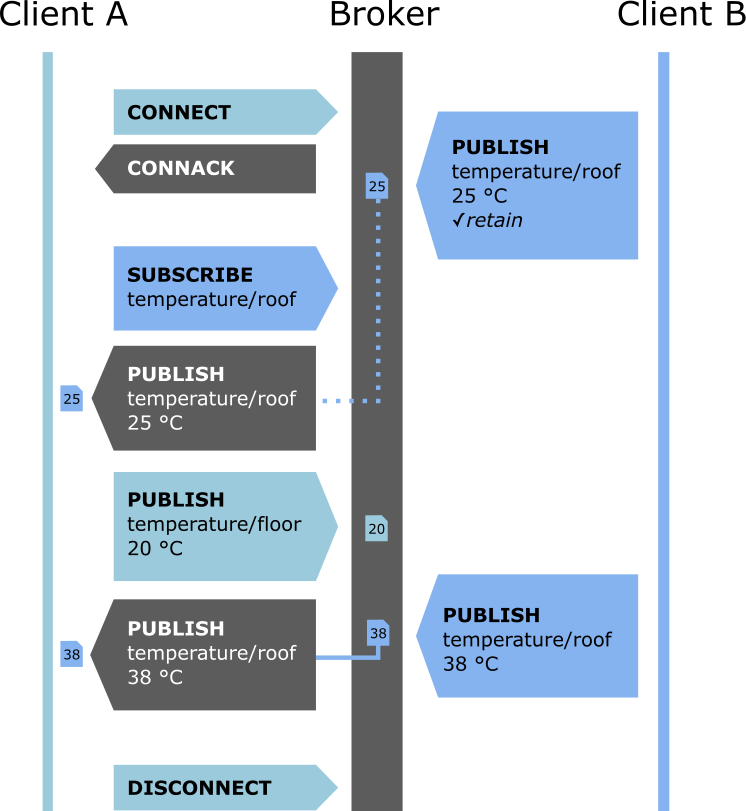
\includegraphics[keepaspectratio]{images/MQTT_protocol_example_without_QoS.png}}
\caption{Fonte: Wikimedia Commons --- Il flusso completo: Client A si
connette (CONNECT/CONNACK), Client B si sottoscrive al topic
\protect\texttt{temperature/roof} (SUBSCRIBE), Client A pubblica tre
misurazioni (20°C, 25°C, 38°C) con flag retain, il broker le inoltra a
Client B.}
\end{figure}

MQTT adotta il paradigma pub/sub con filtraggio basato su topic
organizzati gerarchicamente. L'infrastruttura opera ai livelli
applicativi (5-6 del modello ISO/OSI), sopra TCP (livello 4) e IP
(livello 3). Tutti i dispositivi devono conoscere in anticipo hostname e
porta del broker. Le librerie client gestiscono quasi sempre le
operazioni asincronamente tramite \emph{callback}, pur non precludendo
API sincrone.

\subsection{L'Instaurazione della
Connessione}\label{linstaurazione-della-connessione}

L'interazione tra client e broker inizia quando il client invia un
messaggio \textbf{CONNECT}, che contiene i seguenti parametri:

\begin{itemize}
\tightlist
\item
  \textbf{Client ID} (obbligatorio): stringa univoca che identifica il
  client presso il broker. Se lasciato vuoto, il broker assegna un ID
  automatico, ma non conserverà alcuno stato persistente; in tal caso il
  flag \emph{Clean Session} deve essere impostato a \texttt{true}.
\item
  \textbf{Clean Session} (opzionale): se impostato a \texttt{false}, il
  client richiede una \emph{persistent session} --- il broker salva le
  sottoscrizioni e i messaggi non consegnati (con QoS ≥ 1) e li
  ripristina alla successiva riconnessione con lo stesso Client ID. Con
  \texttt{true}, la sessione è effimera e il broker rimuove ogni stato
  precedente.
\item
  \textbf{Username/Password} (opzionali): per l'autenticazione. Senza
  TLS/SSL transitano in chiaro.
\item
  \textbf{Will flags} (opzionali): definiscono il ``testamento'' del
  nodo --- istruiscono il broker a inviare un avviso agli altri client
  nel caso di disconnessione anomala (\emph{ungraceful disconnect}).
\item
  \textbf{KeepAlive} (opzionale): intervallo in secondi (campo a 16 bit)
  entro cui il client si impegna a inviare almeno un pacchetto di
  controllo (ping). È il meccanismo primario con cui il broker rileva le
  disconnessioni fisiche. Il valore \texttt{0} disabilita il meccanismo.
\end{itemize}

Il broker risponde con un pacchetto \textbf{CONNACK} (\emph{Connect
Acknowledgement}) che include il flag \emph{Connection Accepted} o
\emph{Connection Refused} (per violazione del protocollo, ID non valido
o credenziali errate) e il flag \emph{Session Present}, che indica se il
broker conservava già una sessione persistente per quel client.

\subsection{Sottoscrizione e
Ricezione}\label{sottoscrizione-e-ricezione}

Per abilitare la ricezione dei dati, un client invia al broker un
pacchetto \textbf{SUBSCRIBE} contenente un \texttt{packetId} (per
mappare la risposta attesa) e un elenco di topic da sottoscrivere,
ciascuno con il proprio livello massimo di QoS desiderato.

Il broker risponde con un pacchetto \textbf{SUBACK} che riporta lo
stesso \texttt{packetId} e un \texttt{returnCode} per ogni topic: il
valore \texttt{128} indica fallimento (permessi assenti o topic
malformato); i valori \texttt{0}, \texttt{1} o \texttt{2} indicano
successo, comunicando il \emph{maximum QoS granted}, che può essere
inferiore a quello richiesto. Per revocare una sottoscrizione si usa il
pacchetto \textbf{UNSUBSCRIBE} (con \texttt{packetId} e lista di topic),
a cui il broker risponde con \textbf{UNSUBACK}.

\subsection{Gestione e Best Practices dei
Topic}\label{gestione-e-best-practices-dei-topic}

I \textbf{topic} sono stringhe gerarchiche in cui ogni livello è
separato dal carattere \texttt{/}. Un esempio tipico è
\texttt{home/firstfloor/bedroom/presence}. I subscriber possono usare
due tipi di \textbf{wildcard}:

\begin{itemize}
\tightlist
\item
  \textbf{\texttt{+}}: sostituisce un singolo livello. Ad esempio
  \texttt{home/firstfloor/+/presence} corrisponde a tutti i sensori di
  presenza al primo piano, indipendentemente dalla stanza.
\item
  \textbf{\texttt{\#}}: sostituisce tutti i livelli successivi. Ad
  esempio \texttt{home/firstfloor/\#} cattura qualsiasi dato proveniente
  dal primo piano.
\end{itemize}

I topic che iniziano con \texttt{\$} sono riservati al broker per
statistiche interne del sistema (es. \texttt{\$SYS/broker/uptime},
\texttt{\$SYS/broker/clients/connected}). I client non possono
pubblicare su questi topic.

\begin{calloutwarning}{Best practices per i topic}

\begin{itemize}
\tightlist
\item
  Non iniziare il topic con \texttt{/} (es. \texttt{/home/livingroom} è
  scorretto).
\item
  Non usare spazi nelle stringhe.
\item
  Mantenere le stringhe corte per ridurre l'overhead.
\item
  Usare solo codifiche ASCII o UTF-8.
\item
  Includere il \texttt{clientId} nella gerarchia (es.
  \texttt{sensor1/temperature}) per delimitare logicamente le
  autorizzazioni di pubblicazione.
\item
  Progettare la gerarchia pensando all'espandibilità futura.
\item
  Preferire topic specifici (\texttt{home/livingroom/temperature} e
  \texttt{home/livingroom/humidity}) rispetto ad aggregati generici
  (\texttt{home/livingroom/sensors}).
\item
  Evitare di abusare del wildcard \texttt{\#} nella sottoscrizione: si
  rischia di sommergere il client con troppi messaggi. Ha senso solo per
  storage centralizzato su database.
\end{itemize}

\end{calloutwarning}

\subsection{Pubblicazione e Struttura dei
Messaggi}\label{pubblicazione-e-struttura-dei-messaggi}

Una volta connesso, il publisher può inviare messaggi al broker tramite
pacchetti \textbf{PUBLISH}, ciascuno composto da:

\begin{itemize}
\tightlist
\item
  \textbf{topicName}: stringa che identifica il topic di destinazione,
  usata dal broker per il routing verso i subscriber.
\item
  \textbf{payload}: il contenuto informativo del messaggio. MQTT è
  \emph{data agnostic}, quindi il payload può essere dati binari grezzi,
  testo, XML o JSON --- la scelta è interamente applicativa.
\item
  \textbf{packetId}: identificatore numerico a 16 bit, usato per
  tracciare lo scambio. Vale \texttt{0} per QoS 0 (dove non è
  necessario).
\item
  \textbf{retainFlag}: se attivo, il broker conserva l'ultimo messaggio
  pubblicato su quel topic e lo consegna immediatamente ai nuovi
  subscriber che si iscrivono in seguito.
\item
  \textbf{dupFlag}: indica che il messaggio è un duplicato di uno
  precedente non ancora confermato. Rilevante solo per QoS
  \textgreater{} 0.
\item
  \textbf{qos}: livello di Quality of Service (0, 1 o 2).
\end{itemize}

Una volta inviato il messaggio al broker, il client publisher non ha
responsabilità ulteriori: non sa quanti subscriber stiano ascoltando né
quando riceveranno il dato.

\begin{center}\rule{0.5\linewidth}{0.5pt}\end{center}

\section{I Meccanismi della Quality of Service
(QoS)}\label{i-meccanismi-della-quality-of-service-qos}

Il QoS in MQTT regola il livello di garanzia di consegna dei messaggi
tra client e broker. Un aspetto architetturale importante è che il QoS
sul percorso publisher→broker può essere diverso da quello sul percorso
broker→subscriber: i due segmenti sono indipendenti. Il
\texttt{packetId} è un intero a \textbf{16 bit}, univoco per sessione,
usato per tracciare i messaggi nei livelli con conferme.

\begin{calloutnote}{I tre livelli QoS a confronto}

{\def\LTcaptype{none} % do not increment counter
\begin{longtable}[]{@{}
  >{\raggedright\arraybackslash}p{(\linewidth - 8\tabcolsep) * \real{0.2000}}
  >{\raggedright\arraybackslash}p{(\linewidth - 8\tabcolsep) * \real{0.2000}}
  >{\raggedright\arraybackslash}p{(\linewidth - 8\tabcolsep) * \real{0.2000}}
  >{\raggedright\arraybackslash}p{(\linewidth - 8\tabcolsep) * \real{0.2000}}
  >{\raggedright\arraybackslash}p{(\linewidth - 8\tabcolsep) * \real{0.2000}}@{}}
\toprule\noalign{}
\begin{minipage}[b]{\linewidth}\raggedright
Livello
\end{minipage} & \begin{minipage}[b]{\linewidth}\raggedright
Nome
\end{minipage} & \begin{minipage}[b]{\linewidth}\raggedright
Garanzia
\end{minipage} & \begin{minipage}[b]{\linewidth}\raggedright
Meccanismo
\end{minipage} & \begin{minipage}[b]{\linewidth}\raggedright
Duplicati
\end{minipage} \\
\midrule\noalign{}
\endhead
\bottomrule\noalign{}
\endlastfoot
\textbf{QoS 0} & At most once & Nessuna & Nessun ACK, nessuna
memorizzazione & No \\
\textbf{QoS 1} & At least once & Almeno una consegna & PUBACK &
Possibili \\
\textbf{QoS 2} & Exactly once & Esattamente una consegna & PUBLISH →
PUBREC → PUBREL → PUBCOMP & No \\
\end{longtable}
}

\end{calloutnote}

\subsection{QoS 0 --- At Most Once}\label{qos-0-at-most-once}

QoS 0 è la modalità \emph{best effort}: il messaggio viene inviato una
sola volta senza alcuna conferma (\textbf{ACK}) e senza che il broker lo
memorizzi. Se la connessione cade nel momento sbagliato, il messaggio è
perso. È la scelta corretta per dati che invecchiano rapidamente (es.
letture periodiche di sensori) e per connessioni stabili dove la perdita
occasionale è accettabile.

\subsection{QoS 1 --- At Least Once}\label{qos-1-at-least-once}

QoS 1 garantisce che il messaggio arrivi almeno una volta a
destinazione. Il broker memorizza il messaggio finché non riceve dal
publisher il pacchetto di conferma \textbf{PUBACK}. Se il PUBACK non
arriva entro un certo tempo, il publisher ritrasmette il messaggio con
il flag \texttt{dupFlag} impostato. Questo può generare
\textbf{duplicati}: il subscriber potrebbe ricevere lo stesso messaggio
più volte. QoS 1 è adatto quando nessun dato deve andare perso e il
sistema ricevente è in grado di gestire i duplicati (ad esempio tramite
deduplicazione).

\subsection{QoS 2 --- Exactly Once}\label{qos-2-exactly-once}

QoS 2 è il livello più alto: garantisce che ogni messaggio venga
consegnato \textbf{esattamente una volta}, senza duplicati. Il costo è
un handshake a quattro fasi che aumenta la latenza e l'overhead:

\begin{enumerate}
\def\labelenumi{\arabic{enumi}.}
\tightlist
\item
  \textbf{PUBLISH}: il publisher invia il messaggio al broker.
\item
  \textbf{PUBREC} (\emph{Publish Received}): il broker conferma la
  ricezione e memorizza il messaggio.
\item
  \textbf{PUBREL} (\emph{Publish Release}): il publisher conferma il
  PUBREC e autorizza il broker a procedere con la consegna.
\item
  \textbf{PUBCOMP} (\emph{Publish Complete}): il broker conferma che la
  consegna è avvenuta e che il messaggio può essere eliminato.
\end{enumerate}

Il meccanismo a quattro fasi serve a evitare sia la perdita del
messaggio (gestita da PUBREC) sia la consegna duplicata (gestita da
PUBREL e PUBCOMP). QoS 2 è indicato per applicazioni in cui ogni evento
deve essere processato esattamente una volta --- ad esempio transazioni
finanziarie o comandi critici --- accettando il compromesso su latenza e
throughput.

\begin{center}\rule{0.5\linewidth}{0.5pt}\end{center}

\section{Verso le Sessioni
Persistenti}\label{verso-le-sessioni-persistenti}

Quando un dispositivo IoT si disconnette temporaneamente, il rischio è
di perdere le sottoscrizioni attive e i messaggi nel frattempo
pubblicati sui topic di interesse. Le \textbf{persistent session}
risolvono questo problema: se il flag \emph{Clean Session} è impostato a
\texttt{false} nella fase di CONNECT, il broker mantiene in memoria ---
associato al \texttt{clientId} --- tutte le sottoscrizioni attive e
tutti i messaggi non ancora consegnati con QoS 1 o 2. Alla riconnessione
con lo stesso \texttt{clientId}, la sessione viene ripristinata
automaticamente senza dover ripetere le sottoscrizioni. Questo
meccanismo è fondamentale per dispositivi con connettività intermittente
e getta le basi per le logiche avanzate di gestione dello stato nel
panorama IoT.

\begin{center}\rule{0.5\linewidth}{0.5pt}\end{center}

\newpage

\chapter{MQTT: Affidabilità, Struttura dei Pacchetti e
CoAP}\label{mqtt-affidabilituxe0-struttura-dei-pacchetti-e-coap}

La prima parte della lezione aveva introdotto MQTT come protocollo
publish/subscribe progettato per l'IoT. Qui si approfondiscono i
meccanismi che rendono il protocollo robusto: sessioni persistenti,
messaggi trattenuti, testamento e keep alive. Poi si scende al livello
dei singoli byte che compongono i pacchetti di controllo, si vede
un'implementazione reale su Arduino, e infine si confronta MQTT con HTTP
e con \textbf{CoAP} (\emph{Constrained Application Protocol}),
l'alternativa principale per reti fortemente vincolate.

\begin{center}\rule{0.5\linewidth}{0.5pt}\end{center}

\section{Meccanismi di
Affidabilità}\label{meccanismi-di-affidabilituxe0}

\subsection{Sessioni Persistenti}\label{sessioni-persistenti}

Il problema che le sessioni persistenti risolvono è semplice: un
dispositivo IoT si disconnette spesso --- per risparmio energetico, per
copertura di rete instabile, per reset. Se il broker e il client non
ricordano nulla di ciò che è avvenuto, ogni riconnessione equivale a
ricominciare da zero, perdendo iscrizioni ai topic e messaggi accumulati
durante l'assenza.

\begin{calloutdefinition}{Sessione Persistente (Persistent Session)}

Meccanismo che richiede al broker --- e al client --- di conservare lo
stato operativo attraverso disconnessioni e successive riconnessioni.
Viene attivata dal client al momento della connessione impostando il
flag \textbf{\texttt{cleanSession\ =\ false}} nel pacchetto CONNECT. Il
broker ne conferma la creazione o la ripresa tramite il messaggio
\textbf{CONNACK}.

\end{calloutdefinition}

Quando una sessione persistente è attiva, il broker memorizza le
iscrizioni ai topic del client, i messaggi con QoS 1 e 2 che non è stato
possibile consegnare durante l'assenza, e i messaggi in attesa di
completamento del flusso di acknowledgment QoS 2. Simmetricamente, anche
il \textbf{client} deve salvare stato localmente: tutti i messaggi
inviati ma non ancora confermati dal broker (non-acked), e tutti i
messaggi ricevuti con QoS 2 per i quali non è ancora stata inviata la
conferma. Lo stato viene conservato finché le risorse di sistema lo
consentono.

\begin{calloutwarning}{Quando NON usare le sessioni persistenti}

Non servono per client che pubblicano soltanto con QoS 0, perché in quel
caso non c'è nulla da conservare. Vanno evitate anche quando la
ricezione di messaggi vecchi è indesiderata, o quando il sistema è
progettato per tollerare la perdita di dati senza conseguenze sulla
logica applicativa.

\end{calloutwarning}

\subsection{\texorpdfstring{Messaggi Trattenuti (\emph{Retained
Messages})}{Messaggi Trattenuti (Retained Messages)}}\label{messaggi-trattenuti-retained-messages}

Nel paradigma publish/subscribe, un publisher non ha garanzia che i suoi
messaggi raggiungano i subscriber --- l'unica certezza che può ottenere,
con QoS 1 o 2, è che il broker li abbia ricevuti. Di conseguenza, un
client che si iscrive a un topic non sa quando arriverà il primo
messaggio: potrebbe aspettare ore se il publisher aggiorna raramente.
Questo è un problema reale per qualsiasi dato di stato che cambia di
rado.

La soluzione è il \textbf{retained message}: un normale messaggio con il
flag \texttt{retainFlag\ =\ true}. Quando il broker lo riceve, lo
conserva. Se arriva un nuovo messaggio trattenuto sullo stesso topic, il
broker sostituisce il precedente con l'ultimo --- ne esiste sempre al
massimo uno per topic. Il vantaggio si manifesta alla sottoscrizione:
non appena un client si iscrive a un topic che possiede un messaggio
trattenuto, il broker lo recapita immediatamente, senza attendere la
prossima pubblicazione fisiologica. Questo funziona anche con le
wildcard.

\begin{callouttip}{Esempio: stato di un dispositivo domestico}

Un dispositivo pubblica il proprio stato su
\texttt{home/devices/device1/status} con il payload \texttt{"ON"} e
\texttt{retainFlag\ =\ true}. Quando un nuovo client si iscrive a quel
topic --- anche ore dopo --- riceve immediatamente \texttt{"ON"}, senza
aspettare il prossimo aggiornamento. Per cancellare il messaggio
trattenuto, il publisher invia un messaggio vuoto con
\texttt{retainFlag\ =\ true} sullo stesso topic.

\end{callouttip}

È importante non confondere i retained messages con le sessioni
persistenti: sono meccanismi ortogonali. I messaggi trattenuti vivono
sul broker indipendentemente dalle sessioni dei client, e persistono
anche dopo la consegna.

\subsection{Last Will \& Testament}\label{last-will-testament}

Quando un dispositivo si disconnette \emph{normalmente} --- inviando un
pacchetto DISCONNECT --- gli altri partecipanti possono essere
notificati esplicitamente. Ma quando la disconnessione è anomala (crash
hardware, interruzione di rete, timeout di keep alive), il dispositivo
non ha modo di comunicare il proprio stato. Il meccanismo del
\textbf{Last Will \& Testament} (\emph{testamento}) risolve esattamente
questo scenario.

\begin{calloutdefinition}{Last Will \& Testament}

Messaggio pre-configurato che il client consegna al broker al momento
della connessione (CONNECT time). Se il broker rileva una disconnessione
anomala del client, pubblica automaticamente quel messaggio sul topic
specificato, notificando tutti gli iscritti.

\end{calloutdefinition}

Il testamento è a tutti gli effetti un messaggio MQTT completo: ha un
topic, un payload, un livello di QoS e un retained flag. Il broker lo
memorizza dal momento della connessione e lo invia in quattro
circostanze: errore di I/O sulla connessione di rete, mancato invio del
PINGREQ entro l'intervallo di keep alive, chiusura brusca della
connessione TCP senza DISCONNECT, oppure chiusura forzata da parte del
broker per errore di protocollo. Se invece il client termina la sessione
correttamente con DISCONNECT, il testamento viene scartato.

I quattro parametri del testamento si dichiarano nel messaggio CONNECT:
\textbf{\texttt{lastWillTopic}} (stringa del topic),
\textbf{\texttt{lastWillQoS}} (livello 0, 1 o 2),
\textbf{\texttt{lastWillMessage}} (payload testuale) e
\textbf{\texttt{lastWillRetain}} (booleano).

\begin{callouttip}{Sinergia tra Last Will e Retained Messages}

Il pattern più potente combina i due meccanismi. Riprendendo l'esempio
precedente: il dispositivo pubblica \texttt{"ON"} come retained message
su \texttt{home/devices/device1/status}. Configura anche un testamento
con payload \texttt{"OFF"}, retained flag attivo, sullo stesso topic. Se
va in crash, il broker pubblica automaticamente \texttt{"OFF"} come
retained message --- sia i client connessi che quelli futuri vedranno lo
stato corretto del dispositivo.

\end{callouttip}

\subsection{Keep Alive}\label{keep-alive}

Il \textbf{Keep Alive} affronta un problema specifico del TCP: una
connessione può sembrare attiva anche quando il peer è irraggiungibile,
finché non si tenta di trasmettere. In un sistema IoT con dispositivi
che si connettono e scompaiono, il broker ha bisogno di un modo per
accorgersi tempestivamente delle disconnessioni silenti.

Il client dichiara un intervallo di keep alive nel pacchetto CONNECT. È
suo obbligo inviare un pacchetto \textbf{PINGREQ} al broker prima che
quell'intervallo scada --- qualunque messaggio trasmesso vale come
segnale di vita, non solo il PINGREQ. Il broker risponde con
\textbf{PINGRESP}. Se il client non invia nulla entro il timeout, il
broker chiude la connessione e, se configurato, invia il messaggio di
last will.

\begin{center}\rule{0.5\linewidth}{0.5pt}\end{center}

\section{Struttura dei Pacchetti
MQTT}\label{struttura-dei-pacchetti-mqtt}

Comprendere la struttura dei pacchetti è utile sia per il debug a basso
livello che per capire perché MQTT è così leggero. Ogni \textbf{MQTT
Control Packet} si compone di tre parti: un \textbf{Fixed Header}
(sempre presente), un \textbf{Variable Header} (presente solo in alcuni
tipi di pacchetto) e un \textbf{Payload} (dipendente dal tipo).

\subsection{Fixed Header}\label{fixed-header}

Il Fixed Header occupa almeno 2 byte. Il \textbf{primo byte} codifica
due informazioni: i bit 7--4 contengono il tipo di pacchetto (4 bit → 16
valori possibili, di cui 0 e 15 sono riservati); i bit 3--0 contengono
flag specifici per tipo. Il \textbf{secondo byte} --- eventualmente
seguito da altri --- rappresenta la \emph{Remaining Length}, cioè la
dimensione combinata di variable header e payload. Il campo usa una
codifica a lunghezza variabile: un singolo byte copre fino a 127 byte, e
il bit più significativo segnala la presenza di un byte aggiuntivo di
lunghezza.

\begin{calloutnote}{Flag del primo byte}

Per la maggior parte dei pacchetti i 4 bit di flag sono riservati e
devono valere \texttt{0,0,0,0}. Il pacchetto PUBLISH è l'eccezione:
codifica nei flag i parametri \textbf{DUP} (primo bit), \textbf{QoS}
(due bit centrali) e \textbf{Retain} (ultimo bit). I pacchetti PUBREL,
SUBSCRIBE e UNSUBSCRIBE richiedono invece il valore fisso
\texttt{0,0,1,0}.

\end{calloutnote}

I tipi di pacchetto e la direzione del flusso sono:

{\def\LTcaptype{none} % do not increment counter
\begin{longtable}[]{@{}lll@{}}
\toprule\noalign{}
Valore & Tipo & Direzione \\
\midrule\noalign{}
\endhead
\bottomrule\noalign{}
\endlastfoot
1 & CONNECT & Client → Server \\
2 & CONNACK & Server → Client \\
3 & PUBLISH & Bidirezionale \\
4--7 & PUBACK, PUBREC, PUBREL, PUBCOMP & Bidirezionale (gestione QoS) \\
8 & SUBSCRIBE & Client → Server \\
9 & SUBACK & Server → Client \\
10 & UNSUBSCRIBE & Client → Server \\
11 & UNSUBACK & Server → Client \\
12 & PINGREQ & Client → Server \\
13 & PINGRESP & Server → Client \\
14 & DISCONNECT & Client → Server \\
\end{longtable}
}

\subsection{Variable Header e Payload}\label{variable-header-e-payload}

Il \textbf{Variable Header} contiene principalmente il \textbf{packet
identifier} (2 byte), un identificativo numerico univoco usato per
correlare i pacchetti di acknowledgment. CONNECT e CONNACK non includono
questo campo. Per PUBLISH, è presente solo se QoS \textgreater{} 0.
L'header variabile trasporta anche informazioni aggiuntive dipendenti
dal tipo: in CONNECT, ad esempio, include nome e versione del protocollo
più vari flag operativi.

Il \textbf{Payload} è il corpo del messaggio. Nel CONNECT è obbligatorio
e deve contenere il \textbf{client identifier}; può inoltre includere
will topic, will message, username e password. In CONNACK e PUBLISH è
opzionale. Nei pacchetti di puro controllo come PINGREQ, PINGRESP,
DISCONNECT e tutti i pacchetti di acknowledgment QoS il payload è
assente.

\begin{center}\rule{0.5\linewidth}{0.5pt}\end{center}

\section{Implementazione Pratica: MQTT su
Arduino}\label{implementazione-pratica-mqtt-su-arduino}

La libreria più diffusa per MQTT su Arduino è \textbf{PubSubClient}. È
progettata deliberatamente per essere leggera: implementa solo le
funzionalità core di MQTT, senza SSL/TLS, senza supporto a QoS 2, e con
un limite rigido di 128 byte per il payload. Questi vincoli la rendono
adatta ai microcontrollori a basse risorse tipici dell'ecosistema
Arduino.

\subsection{Costruzione del client}\label{costruzione-del-client}

La libreria si istanzia con il costruttore completo
\texttt{PubSubClient(server,\ port,\ callback,\ client,\ stream)}, dove
\texttt{server} è l'\texttt{IPAddress} del broker, \texttt{port} è un
intero, \texttt{callback} è un puntatore a funzione che viene invocata
all'arrivo di un messaggio, \texttt{client} è un'istanza di rete
(tipicamente \texttt{EthernetClient}), e \texttt{stream} è opzionale per
lo storage dei messaggi ricevuti. È anche possibile usare il costruttore
vuoto e configurare i parametri successivamente via setter
(\texttt{setServer}, \texttt{setCallback}, \texttt{setClient},
\texttt{setStream}).

\begin{calloutnote}{Callback}

Il meccanismo di callback funziona come nelle interfacce grafiche con
gli event listener: la funzione viene eseguita solo quando arriva un
messaggio su un topic sottoscritto. Non c'è polling attivo.

\end{calloutnote}

\subsection{API principale}\label{api-principale}

\texttt{connect(clientID,\ username,\ password,\ willTopic,\ willQoS,\ willRetain,\ willMessage)}
avvia la connessione specificando credenziali e parametri del
testamento; restituisce \texttt{true} in caso di successo.
\texttt{disconnect()} chiude la sessione in modo pulito.

\texttt{publish(topic,\ payload,\ length,\ retained)} pubblica un
messaggio; restituisce \texttt{false} se la connessione è caduta o il
payload supera il limite. \texttt{subscribe(topic,\ qos)} e
\texttt{unsubscribe(topic)} gestiscono le iscrizioni, entrambe con
valore di ritorno booleano.

Fondamentale è la chiamata ripetuta a \textbf{\texttt{loop()}} nel ciclo
principale: è questa funzione che genera i PINGREQ e mantiene viva la
connessione. Senza di essa il broker considererà il client disconnesso
entro l'intervallo di keep alive. I metodi \texttt{connected()} e
\texttt{state()} supportano il debugging.

\begin{center}\rule{0.5\linewidth}{0.5pt}\end{center}

\section{MQTT vs HTTP e il Problema della
Scalabilità}\label{mqtt-vs-http-e-il-problema-della-scalabilituxe0}

MQTT e HTTP sono i principali competitor nell'IoT, ma operano su
paradigmi radicalmente diversi. HTTP impone un'architettura
\textbf{client/server} rigida e simmetrica: ogni entità deve essere o
client o server. Organizzare una rete IoT con HTTP significa che ogni
sensore deve agire da server (o da client che interroga un server
centrale), e che ogni comunicazione è strettamente 1-a-1. Con centinaia
o migliaia di dispositivi, il numero di connessioni simultanee al server
centrale cresce proporzionalmente --- e con esso il carico di risorse.
\textbf{HTTP non scala bene}.

MQTT invece, grazie al publish/subscribe, fa crescere il numero di
connessioni solo sul broker, non sui client. Un nuovo subscriber si
aggiunge alla rete senza che nessun publisher debba sapere della sua
esistenza. Il broker gestisce il \emph{fan-out} internamente.

Dal punto di vista tecnico, MQTT invia dati come array di byte con
header compatti (pochi byte), mentre HTTP trasmette documenti con header
testuali voluminosi. MQTT supporta tre livelli di QoS e topologie 1-a-0,
1-a-1 e 1-a-N; HTTP ha un solo livello di servizio e comunicazione
esclusivamente 1-a-1.

\begin{calloutwarning}{Limiti strutturali di MQTT}

Nonostante i vantaggi, MQTT presenta tre criticità architetturali
importanti. Prima: il broker è un \textbf{single point of failure} ---
se cade, l'intera rete smette di comunicare. Seconda: al crescere della
rete, l'overhead computazionale del broker può diventare incompatibile
con le risorse dei dispositivi finali più vincolati. Terza: MQTT si
appoggia a \textbf{TCP}, che richiede risorse considerevolmente
superiori a UDP, causa tempi di risveglio (\emph{wake-up time}) elevati
per la procedura di handshake, e accorcia la vita della batteria dei
dispositivi che devono mantenere connessioni persistenti.

\end{calloutwarning}

\begin{center}\rule{0.5\linewidth}{0.5pt}\end{center}

\section{CoAP: L'Alternativa per Reti
Vincolate}\label{coap-lalternativa-per-reti-vincolate}

È proprio il problema del TCP che apre la strada al \textbf{CoAP}
(\emph{Constrained Application Protocol}), standardizzato in RFC 7252.
CoAP è progettato specificamente per operare su nodi computazionalmente
deboli e reti con alta perdita di pacchetti, bandwidth nell'ordine dei
10 kbit/s e dispositivi con poche decine di byte di RAM e ROM. Trova
applicazione naturale in sistemi M2M (\emph{Machine-to-Machine}),
building automation e smart energy.

A differenza di MQTT, CoAP abbraccia un classico paradigma
\textbf{client/server} con un twist: sono i sensori e gli attuatori
periferici ad agire da \emph{server}, mentre i software applicativi
centrali fanno da \emph{client} che li interrogano. L'interfaccia è un
modello \textbf{REST} completo: i sensori espongono risorse tramite URI,
e i client le manipolano con i verbi \textbf{GET, PUT, POST, DELETE} ---
esattamente come nell'HTTP convenzionale, ma con profonde ottimizzazioni
sotto.

\begin{calloutnote}{Caratteristiche tecniche di CoAP}

CoAP utilizza \textbf{UDP/IP} come trasporto invece di TCP, eliminando
l'overhead di connessione. Adotta formati di codifica compatti con
header di dimensioni ridottissime. Include nativamente una
\emph{resource directory} per la scoperta (\emph{discovery}) delle
risorse nella rete. Sul fronte sicurezza, integra meccanismi
crittografici robusti --- la protezione è paragonabile a chiavi RSA da
3072 bit. Prospera nelle \textbf{6LoWPAN} (reti IPv6 over Low-Power
Wireless PAN), ambienti con packet error rate elevato e throughput
limitato.

\end{calloutnote}

CoAP supporta anche un modello di comunicazione asincrona che ne
avvicina il comportamento a MQTT, e ha un supporto nativo (seppur
minoritario) per trasmissioni multicast. Il supporto formale di Eclipse
ne accelera la diffusione.

\begin{callouttip}{Quando scegliere CoAP vs MQTT}

Scegli \textbf{MQTT} quando l'obiettivo è massimizzare il
disaccoppiamento tra produttori e consumatori di dati --- nel tempo e
nello spazio --- e quando il broker centralizzato non è un vincolo
architetturale. Scegli \textbf{CoAP} quando lo scenario richiede
sicurezza crittografica forte \emph{by default}, quando si lavora su
reti UDP con dispositivi ultra-vincolati, o quando si vuole evitare la
dipendenza da un broker centrale.

\end{callouttip}

Entrambi i protocolli hanno oggi lo status di standard riconosciuti per
l'IoT. CoAP è più giovane e i suoi meccanismi di affidabilità della
consegna sono meno sofisticati della gerarchia QoS di MQTT, ma la sua
leggerezza e la base UDP lo rendono insostituibile negli scenari più
vincolati.

\begin{center}\rule{0.5\linewidth}{0.5pt}\end{center}

\newpage

\chapter{The ZigBee Standard --- Part
1}\label{the-zigbee-standard-part-1}

\section{Obiettivi e Caratteristiche}\label{obiettivi-e-caratteristiche}

Lo standard \textbf{ZigBee} è un protocollo di comunicazione concepito
specificamente per le reti di sensori wireless (\textbf{wireless sensor
networks}), sviluppato e promosso dalla \textbf{ZigBee Alliance}. Le sue
applicazioni spaziano dalla \textbf{home automation} (domotica e
\emph{ambient assisted living}) all'assistenza sanitaria (\textbf{health
care}), dall'elettronica di consumo all'automazione industriale, fino a
impieghi estremi come le missioni di esplorazione su Marte.

\begin{figure}
\centering
\pandocbounded{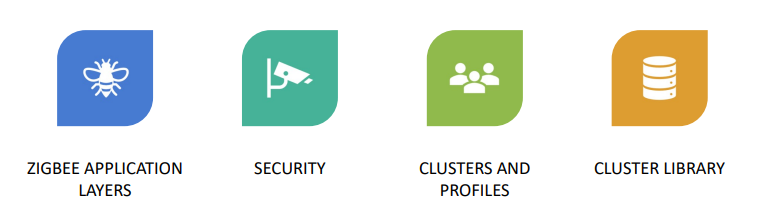
\includegraphics[keepaspectratio]{images/Pasted-image-20260309111850.png}}
\caption{Panoramica delle applicazioni ZigBee nei diversi domini.}
\end{figure}

I requisiti di progetto (\textbf{main requirements}) che ZigBee deve
soddisfare sono tre: la rete deve operare in modo completamente autonomo
senza intervento umano, i dispositivi devono avere una durata della
batteria molto elevata lavorando a basso data rate, e deve essere
garantita la piena interoperabilità tra dispositivi di produttori
differenti.

Le caratteristiche principali (\textbf{main features}) che ne derivano
sono coerenti con questi requisiti: ZigBee è basato su standard aperti,
ha costi ridotti, può essere impiegato globalmente, è affidabile e
auto-rigenerante (\emph{self-healing}), scala a un numero elevato di
nodi, è facile da distribuire sul campo e garantisce sicurezza delle
comunicazioni insieme a una lunghissima durata della batteria.

\begin{center}\rule{0.5\linewidth}{0.5pt}\end{center}

\section{Rapporto con IEEE 802.15.4 e Architettura a
Strati}\label{rapporto-con-ieee-802.15.4-e-architettura-a-strati}

ZigBee è costruito sopra lo standard \textbf{IEEE 802.15.4}, rilasciato
nel 2003 e revisionato nel 2006. ZigBee stesso è stato pubblicato per la
prima volta a fine 2004 e revisionato nel 2006; entrambe le prime
revisioni sono distribuite gratuitamente.

\begin{figure}
\centering
\pandocbounded{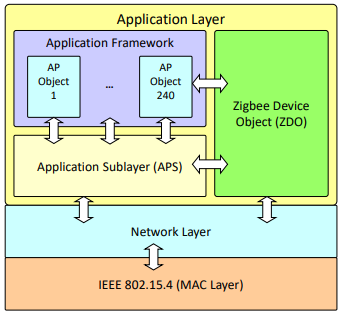
\includegraphics[keepaspectratio]{images/Pasted-image-20260309111918.png}}
\caption{Corrispondenza tra i livelli ISO/OSI e gli standard IEEE
802.15.4 e ZigBee.}
\end{figure}

In termini di stack protocollare, IEEE 802.15.4 copre il
\textbf{Physical layer} e il \textbf{MAC layer}, gestendo reti a basso
data rate definite \emph{Wireless Personal Area Networks}. Questo
standard è infrastructure-less, a corto raggio, supporta topologie a
stella e peer-to-peer e può coesistere con IEEE 802.11 e Bluetooth (IEEE
802.15.1). Opera su bande di frequenza libere da licenza: 868--868.6 MHz
(Europa) a 20 kbps, 902--928 MHz (Nord America) a 40 kbps, e
2400--2483.5 MHz (mondiale) a 250 kbps.

ZigBee aggiunge sopra questi livelli il \textbf{Network layer} e
l'\textbf{Application layer}. Il livello applicativo è articolato in tre
componenti: l'\textbf{Application Framework}, che ospita fino a 240
\textbf{Application Objects (APO)} numerati da 1 a 240, ciascuno
rappresentante un'applicazione ZigBee definita dall'utente; il
\textbf{ZigBee Device Object (ZDO)}, che fornisce i servizi per
organizzare gli APO in un'applicazione distribuita; e
l'\textbf{Application Support sublayer (APS)}, che eroga servizi di dati
e gestione sia agli APO sia allo ZDO.

\begin{center}\rule{0.5\linewidth}{0.5pt}\end{center}

\section{Servizi e Primitive di
Comunicazione}\label{servizi-e-primitive-di-comunicazione}

Ogni livello dello stack eroga servizi di dati e di gestione al livello
superiore tramite quattro tipologie di \textbf{Service Primitives}. La
\textbf{Request} è invocata dal livello superiore per richiedere un
servizio al livello inferiore. L'\textbf{Indication} è generata dal
livello inferiore verso quello superiore per notificare il verificarsi
di un evento. La \textbf{Response} è invocata dal livello superiore per
completare una procedura iniziata da una precedente Indication. La
\textbf{Confirm} è generata dal livello inferiore per comunicare al
livello superiore l'esito di una o più Request precedenti. Non tutti i
servizi utilizzano tutte e quattro le primitive.

In uno schema di comunicazione end-to-end, un oggetto applicativo
incapsula i dati in un \textbf{APDU}, che passa al servizio dati APS
diventando \textbf{NPDU}. Il livello \textbf{NWK} aggiunge le proprie
intestazioni producendo un \textbf{MPDU} tramite il NWK data service; il
livello \textbf{MAC} genera la \textbf{PPDU} tramite il MAC data
service, che viene infine trasmessa fisicamente dal \textbf{PHY} data
service verso la destinazione, dove il processo si inverte.

\begin{figure}
\centering
\pandocbounded{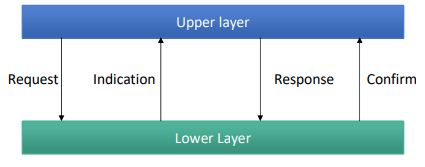
\includegraphics[keepaspectratio]{images/Pasted-image-20260309111946.png}}
\caption{Flusso di incapsulamento dei dati attraverso i livelli dello
stack ZigBee, da sorgente a destinazione.}
\end{figure}

\begin{center}\rule{0.5\linewidth}{0.5pt}\end{center}

\section{Il Network Layer: Topologie e
Servizi}\label{il-network-layer-topologie-e-servizi}

\subsection{Tipologie di Dispositivi}\label{tipologie-di-dispositivi}

Il Network Layer definisce tre ruoli distinti. Il \textbf{Network
Coordinator} è un dispositivo completamente funzionale (\textbf{FFD},
\emph{full functional device}) che crea e gestisce l'intera rete. I
\textbf{Router} sono anch'essi FFD e dispongono di capacità di
instradamento. Gli \textbf{End-device} sono dispositivi a funzionalità
ridotta (\textbf{RFD}, \emph{reduced functional device}) o FFD che
operano come nodi semplici senza capacità di routing.

Le topologie gestite dal Network Layer sono tre. La topologia a
\textbf{stella} si mappa direttamente sulla struttura IEEE 802.15.4 e
utilizza il meccanismo del \emph{superframe}. La topologia ad
\textbf{albero} può anch'essa avvalersi del superframe. La topologia a
\textbf{mesh} opera invece tipicamente senza superframe, affidandosi a
comunicazioni dirette nodo-nodo.

\subsection{Tabella dei Servizi}\label{tabella-dei-servizi}

{\def\LTcaptype{none} % do not increment counter
\begin{longtable}[]{@{}
  >{\raggedright\arraybackslash}p{(\linewidth - 8\tabcolsep) * \real{0.1667}}
  >{\centering\arraybackslash}p{(\linewidth - 8\tabcolsep) * \real{0.0873}}
  >{\centering\arraybackslash}p{(\linewidth - 8\tabcolsep) * \real{0.1111}}
  >{\centering\arraybackslash}p{(\linewidth - 8\tabcolsep) * \real{0.0873}}
  >{\raggedright\arraybackslash}p{(\linewidth - 8\tabcolsep) * \real{0.5476}}@{}}
\toprule\noalign{}
\begin{minipage}[b]{\linewidth}\raggedright
\textbf{Name}
\end{minipage} & \begin{minipage}[b]{\linewidth}\centering
\textbf{Request}
\end{minipage} & \begin{minipage}[b]{\linewidth}\centering
\textbf{Indication}
\end{minipage} & \begin{minipage}[b]{\linewidth}\centering
\textbf{Confirm}
\end{minipage} & \begin{minipage}[b]{\linewidth}\raggedright
\textbf{Description}
\end{minipage} \\
\midrule\noalign{}
\endhead
\bottomrule\noalign{}
\endlastfoot
\textbf{DATA} & X & X & X & Trasmissione dati. \\
\textbf{NETWORK-DISCOVERY} & X & & X & Ricerca di PAN esistenti. \\
\textbf{NETWORK-FORMATION} & X & & X & Creazione di una nuova PAN
(coordinator). \\
\textbf{PERMIT-JOINING} & X & & X & Consente l'associazione di nuovi
dispositivi alla PAN. \\
\textbf{START-ROUTER} & X & & X & (Re-)inizializza il superframe del
coordinator o di un router. \\
\textbf{JOIN} & X & X & X & Richiesta di unirsi a una PAN esistente. \\
\textbf{DIRECT-JOIN} & X & & X & Forza un end-device a unirsi alla PAN
del coordinator o di un router. \\
\textbf{LEAVE} & X & X & X & Lasciare una PAN. \\
\textbf{RESET} & X & & X & Resetta il livello di rete. \\
\textbf{SYNC} & X & & X & Sincronizza o estrae dati pendenti dal
coordinator o da un router. \\
\textbf{GET} & X & & X & Legge i parametri del livello di rete. \\
\textbf{SET} & X & & X & Imposta i parametri del livello di rete. \\
\end{longtable}
}

\begin{center}\rule{0.5\linewidth}{0.5pt}\end{center}

\section{Network Formation}\label{network-formation}

Prima di comunicare, un dispositivo ZigBee deve formare una nuova rete
assumendo il ruolo di \textbf{ZigBee Coordinator}, oppure unirsi a una
rete esistente come router o end-device. Il ruolo viene scelto a tempo
di compilazione (\emph{compile-time}).

La \textbf{Network Formation} è avviata dal Coordinator --- solo se non
è già parte di un'altra PAN --- tramite la primitiva
\textbf{NETWORK-FORMATION.request}. Il processo si articola in una
sequenza di interazioni con il livello MAC: dapprima vengono eseguiti un
energy scan e un active scan (tramite \textbf{SCAN.request} e
\textbf{SCAN.confirm}) per identificare il canale meno rumoroso e
verificare l'assenza di reti limitrofe che potrebbero generare
conflitti. Individuato il canale, viene selezionato un \textbf{PAN ID}
non ancora in uso, dopodiché il Coordinator si auto-assegna l'indirizzo
di rete a 16 bit \textbf{0x0000}. Invoca quindi \textbf{SET.request} al
livello MAC per configurare PAN identifier e indirizzo del dispositivo,
e infine emette \textbf{START.request} (confermata da
\textbf{START.confirm}) affinché il MAC inizi a trasmettere i beacon. La
sequenza si chiude con la \textbf{NETWORK-FORMATION.confirm} verso il
livello applicativo.

\begin{center}\rule{0.5\linewidth}{0.5pt}\end{center}

\section{Ingresso in una Rete
Esistente}\label{ingresso-in-una-rete-esistente}

Un dispositivo può unirsi a una rete in due modi: tramite associazione
classica avviata dal dispositivo stesso, oppure tramite \textbf{Direct
join}, in cui è il coordinator o un router a forzare un end-device ad
aggregarsi alla propria PAN.

\subsection{Join through Association
(child-side)}\label{join-through-association-child-side}

Il dispositivo avvia una \textbf{NETWORK-DISCOVERY} emettendo una
\textbf{SCAN.request} di tipo active scan per individuare le PAN
disponibili. Ricevuta la \textbf{NETWORK-DISCOVERY.confirm}, seleziona
la PAN di interesse e invia una \textbf{JOIN.request} contenente
l'identificatore della rete e un flag che indica se intende aggregarsi
come router o come end-device.

A livello NWK, la JOIN.request porta alla selezione di un nodo genitore
\textbf{P} appartenente alla PAN nel vicinato del dispositivo. Il
comportamento varia in base alla topologia: in una rete a stella P è
necessariamente il coordinator e il dispositivo si aggancia come
end-device; nelle topologie ad albero P può essere il coordinator o un
router, e il dispositivo può aggregarsi sia come router sia come
end-device.

Tramite il protocollo di associazione MAC (primitive
\textbf{ASSOCIATE.request} e \textbf{ASSOCIATE.confirm}), il nodo P
assegna al nuovo dispositivo un \textbf{indirizzo breve a 16 bit}
(\emph{short address}), che viene consegnato al livello NWK tramite
\textbf{JOIN.confirm} e utilizzato per tutte le comunicazioni
successive.

\begin{calloutnote}{Direct Join}

Nel Direct Join è il coordinator o un router a prendere l'iniziativa,
forzando un end-device ad aggregarsi alla propria PAN tramite la
primitiva \textbf{DIRECT-JOIN.request}. Non richiede che il dispositivo
target avvii autonomamente una Network Discovery.

\end{calloutnote}

\begin{center}\rule{0.5\linewidth}{0.5pt}\end{center}

\section{Struttura ad Albero e
Indirizzamento}\label{struttura-ad-albero-e-indirizzamento}

Le relazioni genitore-figlio stabilite durante il joining costruiscono
una topologia logica ad albero in cui il Coordinator funge da radice, i
router sono nodi interni (o foglie), e gli end-device sono
esclusivamente foglie.

Questa struttura viene sfruttata per l'assegnazione sistematica degli
indirizzi di rete. Al momento della formazione, il Coordinator viene
configurato con tre parametri statici:

\begin{itemize}
\tightlist
\item
  \(R_m\): numero massimo di router figli per ogni nodo router.
\item
  \(D_m\): numero massimo di end-device figli per ogni nodo router.
\item
  \(L_m\): profondità massima dell'albero.
\end{itemize}

In base a questi valori, ogni router riceve un intervallo specifico di
indirizzi da distribuire ai propri discendenti. L'ampiezza
dell'intervallo assegnato a un router alla profondità \(d\) è calcolata
tramite la funzione ricorsiva \(C_{skip}\):

\[
C_{skip}(d) = \begin{cases} 1 & \text{se } d = L_m \\ 1 + R_m \cdot C_{skip}(d+1) + D_m & \text{altrimenti} \end{cases}
\]

Il valore \(C_{skip}(d)\) rappresenta il numero totale di indirizzi
(incluso il proprio) che ogni router alla profondità \(d\) deve
riservare per sé e per tutti i suoi discendenti. Se un router ha
indirizzo \(A\) e si trova alla profondità \(d\), i suoi \(R_m\) figli
router ricevono rispettivamente gli indirizzi \(A+1\),
\(A+1+C_{skip}(d+1)\), \(A+1+2\cdot C_{skip}(d+1)\), \ldots, e i suoi
\(D_m\) end-device ricevono gli indirizzi successivi a tutti i blocchi
dei router.

\begin{callouttip}{Esempio con R\_m=2, D\_m=2, L\_m=3}

\begin{itemize}
\tightlist
\item
  \(C_{skip}(3) = 1\)
\item
  \(C_{skip}(2) = 1 + 2 \cdot 1 + 2 = 5\)
\item
  \(C_{skip}(1) = 1 + 2 \cdot 5 + 2 = 13\)
\item
  \(C_{skip}(0) = 1 + 2 \cdot 13 + 2 = 29\) → la radice (coordinator,
  \(A=0\)) gestisce \([0\text{–}28]\)
\end{itemize}

Il primo figlio router riceve \(A=1\) e gestisce \([1\text{–}13]\); il
secondo \(A=14\) e gestisce \([14\text{–}26]\); gli end-device del
coordinator sono 27 e 28.

\end{callouttip}

È preferibile che i dispositivi si aggreghino il più in alto possibile
nell'albero per minimizzare il numero di hop. Sebbene gli indirizzi
vengano assegnati secondo una struttura ad albero, la connettività
fisica può comunque formare una mesh.

\begin{calloutwarning}{Rigidità dell’indirizzamento}

Il modello è riconosciuto come rigido: se un sottoalbero è localmente
saturo, un nuovo dispositivo non riesce ad aggregarsi tramite quel nodo.
Il vantaggio è la piena decentralizzazione --- nessun router deve
consultare il coordinator, non esistono rischi di collisione e non sono
necessari algoritmi di accordo distribuito. La connettività fisica può
comunque formare una mesh, anche se gli indirizzi sono distribuiti
secondo logica ad albero.

\end{calloutwarning}

\begin{center}\rule{0.5\linewidth}{0.5pt}\end{center}

\section{Routing}\label{routing}

Il Network Layer supporta tre modalità di instradamento: broadcast,
\textbf{Tree routing} e \textbf{Mesh routing}.

\subsection{Tree Routing}\label{tree-routing}

Nel Tree routing i pacchetti seguono gerarchicamente la struttura
genitore-figlio dell'albero fino alla destinazione, basandosi
esclusivamente sull'indirizzo di rete. È un approccio semplice ma
rigido, e consente l'uso dei beacon poiché ogni router di inoltro
sincronizza il proprio superframe con il nodo limitrofo.

\subsection{Mesh Routing}\label{mesh-routing}

Il Mesh routing è più flessibile e si ispira a protocolli per reti ad
hoc come \textbf{AODV}. Se il mittente è un end-device, il pacchetto
viene inoltrato direttamente al suo nodo genitore. Se il mittente è un
router o il coordinator, viene consultata la \textbf{Routing Table
(RT)}, che contiene per ogni entry il \textbf{Destination Address} (16
bit), il \textbf{Next-hop Address} (16 bit) e l'\textbf{Entry Status} (3
bit: \emph{Active}, \emph{Discovery\_underway},
\emph{Discovery\_failed}, \emph{Inactive}).

Quando nella Routing Table non è presente un'entry valida, il router
avvia il \textbf{Route Discovery Protocol}: viene diffuso in broadcast
un messaggio \textbf{RREQ} (Route Request) contenente l'RREQ ID,
l'indirizzo di destinazione e il path cost inizialmente a 0. I nodi
intermedi propagano l'RREQ aggiornando il \emph{Forward Cost} in base
alle stime di qualità del link fornite dall'interfaccia IEEE 802.15.4.
Un nodo intermedio che conosce già il percorso verso la destinazione
\textbf{può rispondere autonomamente} con un RREP senza attendere la
destinazione; la destinazione risponde sempre. Il \textbf{RREP} (Route
Reply) viene inviato in unicast lungo il percorso inverso: durante il
ritorno ogni nodo aggiorna la propria Routing Table con il
\emph{Residual Cost}. La \textbf{Route Discovery Table (RDT)} traccia
per ogni scoperta: RREQ ID (8 bit), Source Address (16 bit), Sender
Address (16 bit, hop precedente a costo minore), Forward Cost (8 bit,
basato su link quality estimation), Residual Cost (8 bit, compilato dal
RREP) ed Expiration time (16 bit, millisecondi alla scadenza).

\begin{callouttip}{Esempio di Routing Table nel Mesh}

Nella rete con \(R_m=2\), \(D_m=2\), \(L_m=3\), supponiamo che il nodo 3
debba raggiungere il nodo 25. Poiché non esiste un'entry valida, viene
avviato il Route Discovery. Al termine, le routing table risultanti
possono essere:

{\def\LTcaptype{none} % do not increment counter
\begin{longtable}[]{@{}lll@{}}
\toprule\noalign{}
Nodo & Destination & Next-hop \\
\midrule\noalign{}
\endhead
\bottomrule\noalign{}
\endlastfoot
3 & 25 & 15 \\
14 & 25 & 25 \\
25 & --- & --- \\
\end{longtable}
}

Il nodo 3 instrada verso 15 (che ha un link diretto con 25), non
necessariamente seguendo il percorso ad albero.

\end{callouttip}

\begin{callouttip}{Trade-off Mesh vs Tree}

Mesh routing è più robusto e flessibile ma non supporta il beaconing.
Tree routing consente il beaconing ma segue cammini rigidi. Le due
modalità \textbf{possono coesistere nella stessa rete ZigBee}: ogni
router può mantenere sia informazioni per il mesh routing che per il
tree routing, e l'algoritmo di instradamento può passare dinamicamente
da un modo all'altro --- ad esempio usando il tree routing quando il
beaconing è necessario e passando al mesh quando è preferibile un
percorso ottimale.

\end{callouttip}

\begin{center}\rule{0.5\linewidth}{0.5pt}\end{center}

\newpage

\chapter{Lezione 12 --- Application Layer of
ZigBee}\label{lezione-12-application-layer-of-zigbee}

L'\textbf{Application Layer}~del protocollo ZigBee si basa sullo
standard IEEE 802.15.4 e gestisce direttamente i servizi applicativi
della rete.~Questo livello si compone di tre elementi fondamentali:
l'\textbf{Application Framework}, lo~\textbf{ZigBee Device Object
(ZDO)}~e l'\textbf{Application Support Sublayer (APS)}.~L'Application
Framework è l'ambiente in cui risiedono fino a 240~\textbf{Application
Objects (APO)}, ovvero le applicazioni ZigBee definite dall'utente.~Lo
ZDO, invece, fornisce i servizi necessari per organizzare gli APO in
un'applicazione distribuita.~Infine, l'APS fa da tramite offrendo
servizi dati, di scoperta e di gestione (binding) sia agli APO che allo
ZDO.

\pandocbounded{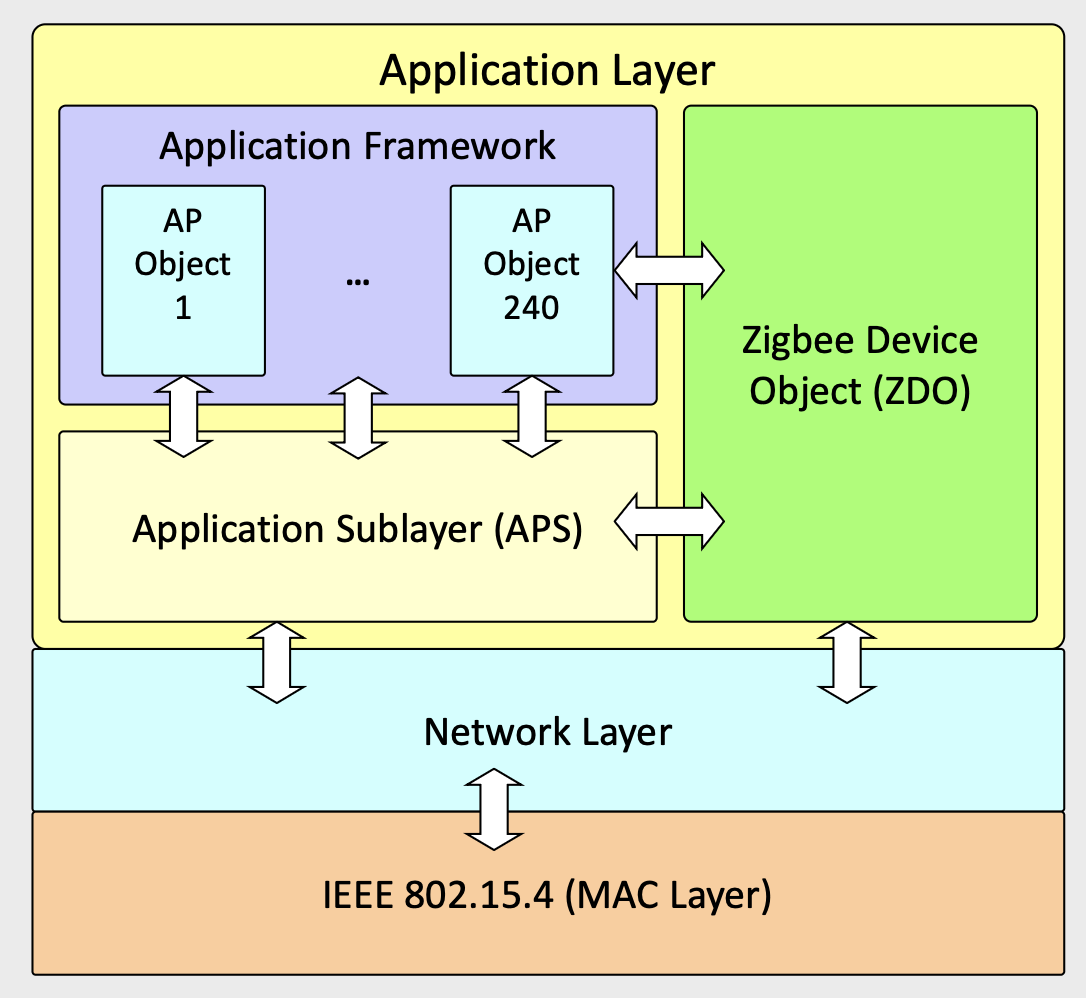
\includegraphics[keepaspectratio]{images/Pasted-image-20260317144430.png}}

\section{L'Application Framework e gli
Endpoints}\label{lapplication-framework-e-gli-endpoints}

All'interno dell'Application Framework, ogni~\textbf{Application Object
(APO)}~è associato a uno specifico~\textbf{Endpoint}, identificato da un
numero compreso tra 1 e 240.~==L'Endpoint 0 è strettamente riservato
allo ZDO==.~Grazie a questo sistema, un singolo dispositivo ZigBee può
eseguire molteplici applicazioni simultaneamente, in quanto gli endpoint
fungono da ``cavi virtuali'' (simili ai socket in Unix) che collegano le
applicazioni e consentono la coesistenza di profili e punti di controllo
distinti su un unico nodo.~Ogni APO è identificato in modo univoco dalla
combinazione tra l'indirizzo di rete del dispositivo ospitante e il suo
numero di endpoint.~Nelle prime versioni di ZigBee, gli APO più semplici
venivano interrogati tramite il servizio~\textbf{Key Value Pair (KVP)},
ora assorbito dalla Cluster Library~, mentre le applicazioni più
complesse comunicano tramite il servizio messaggi.

\begin{calloutimportant}{Focus: Definizione di Cluster e Profilo }

Un~\textbf{Cluster}~è una collezione di comandi e attributi che
definiscono l'interfaccia per una specifica funzionalità del dispositivo
(ad esempio, accendere o spegnere una luce).~È identificato da un codice
a 16 bit, il cui significato dipende dal profilo di
appartenenza.~Un~\textbf{Application Profile}~è invece la specifica del
comportamento di un'intera classe di applicazioni (es.~\emph{Home
Automation}) che possono operare su vari dispositivi ZigBee.~Anche i
profili usano ID a 16 bit: quelli pubblici vanno
da~\(0\times0000\)~a~\(0\times7FFF\), mentre quelli dei produttori
da~\(0\times BF00\)~a~\(0\times FFFF\).~Ogni messaggio inviato in rete è
infatti contrassegnato (tagged) con un Profile ID.

\end{calloutimportant}

\section{I Cluster e i Profili}\label{i-cluster-e-i-profili}

I cluster permettono di interagire con le funzionalità di un APO tramite
protocolli operativi che, nei casi più semplici, prevedono lo scambio di
un singolo messaggio.~I~\textbf{comandi}~innescano azioni fisiche o
logiche sul dispositivo, mentre gli~\textbf{attributi}~ne rivelano lo
stato corrente. Esistono svariati cluster definiti dalla ZigBee Alliance
per ambiti generali.

{\def\LTcaptype{none} % do not increment counter
\begin{longtable}[]{@{}ll@{}}
\toprule\noalign{}
\textbf{Cluster Name} & \textbf{Cluster ID} \\
\midrule\noalign{}
\endhead
\bottomrule\noalign{}
\endlastfoot
Basic Cluster & \(0\times0000\) \\
Power Configuration Cluster & \(0\times0001\) \\
Temperature Configuration Cluster & \(0\times0002\) \\
Identify Cluster & \(0\times0003\) \\
Group Cluster & \(0\times0004\) \\
Scenes Cluster & \(0\times0005\) \\
OnOff Cluster & \(0\times0006\) \\
Level Control Cluster & \(0\times0008\) \\
Time Cluster & \(0\times000A\) \\
Location Cluster & \(0\times000B\) \\
\end{longtable}
}

Anche gli Application Profiles sono standardizzati in un ``domain
space'' per garantire l'interoperabilità in settori specifici:

{\def\LTcaptype{none} % do not increment counter
\begin{longtable}[]{@{}ll@{}}
\toprule\noalign{}
\textbf{Profile ID} & \textbf{Profile name} \\
\midrule\noalign{}
\endhead
\bottomrule\noalign{}
\endlastfoot
0101 & Industrial Plant Monitoring \\
0104 & Home Automation \\
0105 & Commercial Building Automation \\
0107 & Telecom Applications \\
0108 & Personal Home \& Hospital Care \\
0109 & Advanced Metering Initiative \\
\end{longtable}
}

\section{Device IDs}\label{device-ids}

I~\textbf{Device IDs}~sono codici a 16 bit (con range
da~\(0\times0000\)~a~\(0\times FFFF\)) che identificano la tipologia
fisica del dispositivo.~Il loro scopo primario è rendere i dispositivi
riconoscibili agli esseri umani e agli strumenti di diagnosi, ad esempio
per mostrare a display l'icona di un interruttore o di un termostato
anziché un codice illeggibile.

\begin{calloutwarning}{Attenzione: Scoperta dei Servizi e Device IDs }

Un Device ID ti dice solo~\emph{cos'è}~l'oggetto (es. un forno o una
lampadina intelligente), ma non ti indica affatto come poter comunicare
con esso.~Per capirlo devi necessariamente scoprire quali ID dei Cluster
implementa.~Proprio per questo motivo, ==la rete ZigBee non usa i Device
ID per la Service Discovery==: la ricerca avviene interrogando
direttamente i Profile ID e Cluster ID.

\end{calloutwarning}

\section{L'Application Support Sublayer
(APS)}\label{lapplication-support-sublayer-aps}

L'APS funge da livello di trasporto leggero (Light Transport Layer) che
eroga tre tipologie di servizi:~\textbf{Data Service},~\textbf{Binding
Service}~(gestione delle connessioni logiche tra endpoint allo ZDO)
e~\textbf{Group Management}.~Il servizio dati facilita lo scambio di
messaggi e l'affidabilità si basa su tre primitive
fondamentali:~\textbf{request}~(invio),~\textbf{confirm}~(notifica
dell'esito della trasmissione di ritorno)
e~\textbf{indication}~(ricezione al livello destinazione).~L'APS si
occupa attivamente di filtrare i pacchetti per scartare quelli destinati
a endpoint non registrati o profili non compatibili, e ha il compito di
generare gli acknowledgment end-to-end.

\pandocbounded{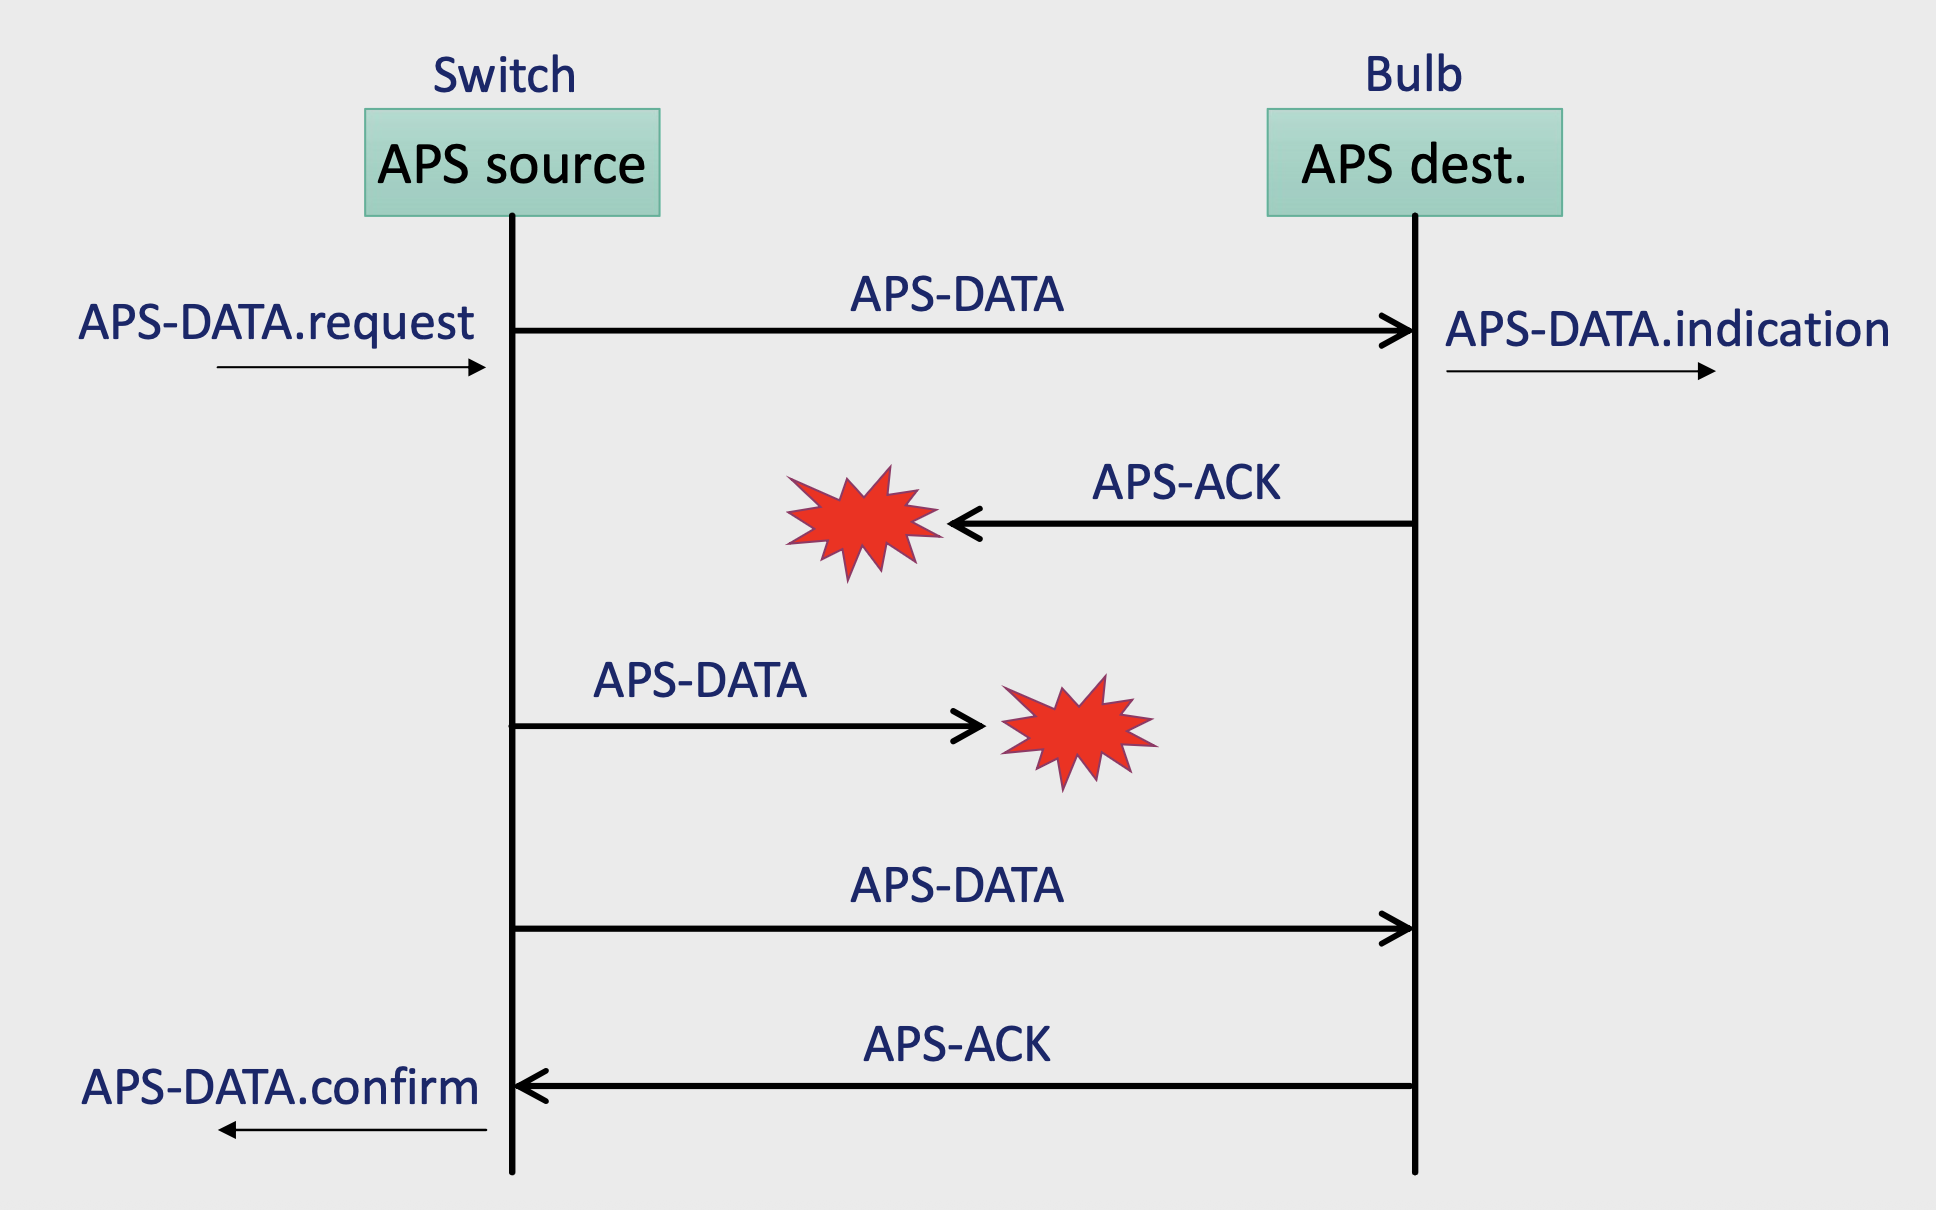
\includegraphics[keepaspectratio]{images/Pasted-image-20260317150017.png}}

Per gestire gruppi di APO e consentire la trasmissione multicast, l'APS
usa le proprie tabelle locali.~Ogni gruppo ha uno specifico indirizzo a
16 bit: le
primitive~\texttt{ADD-GROUP}~e~\texttt{REMOVE-GROUP}~associano
dinamicamente la coppia indirizzo di rete / endpoint al gruppo,
occupandosi di crearlo da zero nel caso non esista ancora.~Tali
informazioni vengono salvate e consultate nelle Group Tables dell'APS.

\section{APS Binding e Indirizzamento
Indiretto}\label{aps-binding-e-indirizzamento-indiretto}

Il~\textbf{Binding}~consente di creare connessioni unidirezionali tra un
endpoint su un nodo sorgente e uno o molteplici endpoint su altri
nodi.~È un meccanismo vitale che può essere configurato solo su
esplicita richiesta dello ZDO di un coordinatore o di un router.

Il grande vantaggio del binding è permettere l'\textbf{indirizzamento
indiretto}.~Dispositivi estremamente semplici o sensori poveri non
necessitano di conoscere la topologia della rete o l'indirizzo esatto di
chi dovrà processare i loro dati.~Tramite le
primitive~\texttt{BIND.request}~e~\texttt{UNBIND.request}, la Binding
Table prende in carico una richiesta in uscita (incrociando l'indirizzo
sorgente e l'ID del cluster in esame) e la mappa automaticamente verso
le corrette
coordinate~\texttt{\textless{}destination\ endpoint,\ destination\ network\ addr\textgreater{}}.

\begin{calloutnote}{Contesto: Cambiamento Indirizzi e Address Map }

Poiché i dispositivi ZigBee acquisiscono gli indirizzi in modo
decentralizzato, in caso di reset o mancanza di corrente un sensore e un
attuatore prima in comunicazione potrebbero risvegliarsi ottenendo nuovi
indirizzi di rete a 16 bit.~Non serve però l'intervento di un tecnico:
l'APS layer usa internamente la~\textbf{Address Map Table}~che associa
stabilmente gli indirizzi 16 bit NWK con gli immutabili indirizzi MAC a
64 bit (IEEE MAC address).~In caso di riavvio il nodo esegue un annuncio
sulla rete e tutti i nodi riaggiornano le tabelle locali in base ai MAC,
ripristinando in modo invisibile i binding indiretti.

\end{calloutnote}

\section{Lo ZigBee Device Object
(ZDO)}\label{lo-zigbee-device-object-zdo}

Lo~\textbf{ZDO}~è la speciale applicazione gestionale del nodo ed è
perennemente attaccato all'Endpoint 0.~Le sue funzionalità e
comportamenti dipendono strettamente dallo~\textbf{ZigBee Device Profile
(ZDP)}, che definisce quali cluster un dispositivo standard deve
supportare e regola le policy di sicurezza, la gestione dei nodi e le
regole di binding. I principali servizi esposti dallo ZDO includono:

\begin{itemize}
\item
  \textbf{Device e Service Discovery:}~La Device Discovery recupera per
  l'utente gli indirizzi fisici MAC o di rete interrogando la rete in
  unicast oppure sfruttando un broadcast gerarchico in cui i router o i
  coordinatori rispondono raggruppando i dispositivi a loro
  associati.~La Service Discovery serve a reperire informazioni sui
  servizi, con richieste filtrate per cluster o ID di profilo, anch'esse
  risolte gerarchicamente dai router padre o in unicast (con i router
  che rispondono per conto dei nodi End Device addormentati).
\item
  \textbf{Binding Management:}~Processa e attua fisicamente tutte le
  richieste di modifica alle tabelle di binding dell'APS da entità
  remote o locali.
\item
  \textbf{Node e Network Management:}~Implementa il comportamento di
  base stabilito per il ruolo del nodo alla configurazione, garantendo
  la gestione ordinata di ingressi (join) e uscite (leave) dalla rete
  dei dispositivi e lo smistamento di informazioni interne sulle routing
  table.
\end{itemize}

\section{La ZigBee Cluster Library
(ZCL)}\label{la-zigbee-cluster-library-zcl}

Per evitare che gli sviluppatori riscrivano codice generico
(``reinventare la ruota''), la ZigBee Alliance ha istituito
la~\textbf{ZigBee Cluster Library (ZCL)}, un gigantesco e aggiornato
repository di funzionalità standardizzate che supporta e facilita
enormemente l'interoperabilità tra dispositivi di terze parti e la
manutenibilità software.~Per esempio, all'interno del dominio domotico
(\emph{Home Automation}), i cluster sono strutturati rigorosamente in
categorie semantiche~: Closures (chiusure, serrature e tende), HVAC
(pompe di calore, deumidificatori e termostati), Lighting (luci),
Measurement and Sensing (sensori ambientali) o Protocol Interfaces
(interfacce di traduzione).

\subsubsection{L'Architettura Client-Server della
ZCL}\label{larchitettura-client-server-della-zcl}

Ogni cluster introdotto dalla ZCL poggia saldamente su un modello
gerarchico Client-Server per l'accesso e la manipolazione di un Dominio
Funzionale:

\begin{itemize}
\item
  \textbf{Il Server}~è colui che ospita fisicamente il dato e ne
  conserva lo stato (memorizza e governa gli~\textbf{attributi}).
\item
  \textbf{Il Client}~è il dispositivo di comando che manipola gli
  attributi e invia istruzioni al Server.~Questa logica supporta
  l'impilamento e permette la compatibilità verso il basso.~In base alla
  propria complessità, per esempio, una ``Lampadina dimmerabile a
  colori'' vestirà simultaneamente i panni del Server nel Cluster
  On/Off, nel Cluster Level Control (luminosità) e nel Color Control,
  esponendo attributi diversi alla rete.
\end{itemize}

\subsubsection{Comandi e Attributi della
ZCL}\label{comandi-e-attributi-della-zcl}

I comandi ZCL consistono tecnicamente in messaggi formattati con un
header e un payload.~I flussi logici consentono di leggere, manipolare o
interrogare le funzionalità, e partono comunemente dal client.~Ma la
vera forza è il~\textbf{Dynamic Attribute Reporting}~: si tratta di
comandi preposti che viaggiano in senso contrario (dal Server al Client
associato) contenenti aggiornamenti sul valore registrato
dall'attributo.~Grazie a regole parametriche precise (si può impostare
una frequenza di aggiornamento, una durata, o notificare le anomalie al
superamento di un valore di tolleranza), il reporting automatico
previene gli sprechi d'energia in trasmissioni superflue.

Includono inoltre interrogazioni standard ai metadati dell'hardware,
basate sul~\textbf{Basic Device Info Cluster}(\(0\times0000\)) e
configurazioni sull'alimentazione tramite il~\textbf{Power Configuration
Cluster}~(\(0\times0001\)), il cui attributo
base~\textbf{PowerSource}~può valere ``Mains (single phase)''
(\(0\times01\)), ``Battery'' (\(0\times03\)) o ``DC Source''
(\(0\times04\)), fino agli UPS di emergenza (\(0\times05\)).

\section{Esempio Applicativo: Indoor
Localization}\label{esempio-applicativo-indoor-localization}

Oltre alle tipiche automazioni, lo standard include funzionalità
ingegnose come l'\textbf{Indoor Localization}~all'interno di
ZigBee.~Attraverso lo scambio di segnali radio, un sensore valuta la
distanza dai nodi adiacenti estrapolandola dalla qualità del segnale
ricevuto misurata dell'hardware (RSSI) e attuando tecniche di
triangolazione spaziale. La rete per farlo si appoggia a due
architetture primarie:

\begin{enumerate}
\def\labelenumi{\arabic{enumi}.}
\item
  \textbf{Remote Positioning:}~Il nodo mobile è una scatola nera che
  invia il suo faro radio (ping).~La rete di sensori statici riceventi
  (le~\emph{ancore}) misura e incrocia le RSSI per scoprire la
  posizione.
\item
  \textbf{Self Positioning:}~La rete di ancore emette messaggi beacon
  continui; il dispositivo mobile intelligente fa una stima triangolando
  internamente i ping ricevuti e scoprendo la propria posizione.
\end{enumerate}

Per esporre i dati agli sviluppatori si utilizza lo
speciale~\textbf{RSSI Location Cluster}~che permette scambi opzionali di
informazioni sulla potenza o sui canali.~Contrariamente a quanto
intuitivo, in questo modello ==il Client è il nodo fisso (l'ancora)
mentre il Server del cluster è proprio il dispositivo Mobile== in quanto
eroga lui i parametri.~L'attributo
essenziale~\texttt{Location\ Method}~(\(0\times0001\)) modella la
tecnica: Laterazione RSSI classica (\(0\times00\)), localizzazione per
Prossimità al ricevitore più vicino (\(0\times01\)), Fingerprinting
incrociando i dati con un database precompilato (\(0\times02\)),
Localizzazione da bande estranee a ZigBee (\(0\times03\)), o
elaborazione demandata a Gateway~\textbf{Centralizzato}~(\(0\times04\))
in cui il nodo centrale raccoglierà tutto lo storico per iniettare
l'esito calcolato nel cluster del dispositivo target tramite il
comando~\texttt{Set\ Absolute\ Location}~(\(0\times00\)).

\section{Wrap-Up: Costruire una Soluzione
ZigBee}\label{wrap-up-costruire-una-soluzione-zigbee}

Creare una linea di prodotti supportati da ZigBee non parte mai da
zero.~L'hardware di base, lo stack con le logiche dei livelli ISO-OSI (e
il relativo ZDO) e gran parte delle librerie della ZCL sono già
sviluppate dai produttori di SoC radio.~Il lavoro dell'azienda si riduce
all'assemblaggio dei trasduttori fisici ai chip, unito alla
configurazione software mirata della classe del dispositivo: si
programma il suo ruolo (Coordinatore, Router o End Device dormiente) e
si instanziano gli specifici APO all'interno dei relativi endpoint per
dare ``cervello logico'' (business logic) agli attributi preposti dalla
ZCL, garantendo così istantanea compatibilità su vasta scala con gli
impianti intelligenti esistenti nel mondo.

\begin{calloutnote}{Glossario}

\begin{itemize}
\item
  \textbf{APO (Application Object):}~L'effettiva applicazione firmware
  scritta per un device ZigBee (es. logica di un termostato).~Risiede
  all'interno dell'Application Framework.
\item
  \textbf{Endpoint:}~È l'indirizzamento logico che connette l'APO alla
  rete come un filo virtuale (da 1 a 240).~Il nodo 0 è sempre dedicato
  per design al gestore di rete ZDO.~-~\textbf{Binding Indiretto:}~Un
  geniale meccanismo dell'APS che crea ponti funzionali logici tra
  sensori e attuatori senza che essi sappiano nulla della rete,
  appoggiandosi alla tabella Binding Table aggiornata dinamicamente coi
  MAC address.~
\item
  \textbf{ZCL (ZigBee Cluster Library):}~Standardizzazione mondiale che
  ordina ogni applicativo in un modello Client/Server rigoroso,
  associando ID (Cluster ID) a un elenco formale di Comandi e Attributi.
\end{itemize}

\end{calloutnote}

\newpage

\chapter{Lezione 13 --- ZigBee
Security}\label{lezione-13-zigbee-security}

La~\textbf{sicurezza}~all'interno dello standard ZigBee si fonda su
un'architettura rigorosa, progettata per fornire quattro servizi
essenziali a ogni nodo: lo stabilimento delle chiavi (\textbf{key
establishment}), il loro trasporto logico (\textbf{key transport}), la
protezione crittografica dei frame dati (\textbf{frame protection}) e la
gestione remota e sicura dei dispositivi (\textbf{device management}).
Queste quattro colonne portanti forniscono i blocchi fondamentali su cui
si regge ogni policy di sicurezza all'interno del protocollo.

\section{Scelte di Design per la
Sicurezza}\label{scelte-di-design-per-la-sicurezza}

Per garantire la robustezza del sistema, ZigBee impone precise e
vincolanti scelte architetturali. In primo luogo, vige la regola per cui
==il livello di rete che genera originariamente un frame è sempre il
diretto responsabile della sua messa in sicurezza iniziale== (ad
esempio, un comando nato a livello NWK deve rigorosamente utilizzare la
NWK security prima di essere inoltrato).

Se l'obiettivo dell'infrastruttura è proteggersi in modo proattivo dal
furto di servizio (\emph{theft of service}), allora la protezione a
livello NWK va applicata in modo tassativo a tutti i frame che
transitano; l'unica eccezione concessa riguarda le delicate fasi
di~\emph{join}~quando un nuovo dispositivo entra nella rete.

L'architettura incoraggia fortemente il riutilizzo pratico del materiale
crittografico tra i vari livelli di uno stesso dispositivo, e consiglia
l'uso di link-key per aggiungere un ulteriore strato di sicurezza che
accompagni il dato per tutto il tragitto end-to-end (dalla sorgente
esatta alla destinazione finale). Un'applicazione software di terze
parti ha sempre la libertà di introdurre meccanismi crittografici
aggiuntivi, ma la loro gestione ricadrà interamente sulle spalle
dell'applicazione stessa, senza coinvolgere il protocollo.

\begin{calloutwarning}{Attenzione: Gestione delle Anomalie}

Ogni~\emph{Application Profile}~sviluppato deve sempre includere
procedure di emergenza per gestire gli errori. Le eccezioni o i
fallimenti nei processi di~\emph{securing}~e~\emph{unsecuring}~dei
pacchetti non vanno mai ignorati, perché spesso sono i primissimi
sintomi di una grave perdita di sincronizzazione del materiale
crittografico o denotano l'attività di un attacco hacker in corso. È di
vitale importanza rilevare tempestivamente le perdite di
sincronizzazione dei contatori o il loro~\emph{overflow}, le perdite di
sincronizzazione delle chiavi stesse, e far scadere proattivamente le
chiavi per forzarne un aggiornamento periodico.

\end{calloutwarning}

\section{L'Architettura di Sicurezza
ZigBee}\label{larchitettura-di-sicurezza-zigbee}

All'interno dello strato ISO-OSI, ogni livello fa la sua parte.
Il~\textbf{Network Layer (NWK)}~ha il preciso compito di garantire il
trasporto sicuro dei propri frame. Sfruttando le chiavi crittografiche
fornite dal livello superiore, il NWK provvede alla cifratura del
messaggio (\emph{encryption}), alla verifica della sua integrità e al
controllo della cosiddetta~\emph{freshness}: un meccanismo per
assicurarsi che il dato sia ``fresco'' (non un duplicato) così da
rigettare i~\emph{replay attacks}. Va però ricordato che, per forza di
cose, alcuni pacchetti operativi (come i primissimi messaggi di
associazione) viaggiano in chiaro.

Salendo, l'\textbf{Application Support Sublayer (APS)}~fa il lavoro
sporco. Deve garantire il trasporto sicuro dei frame a livello APS,
implementare materialmente tutti i protocolli matematici per lo
stabilimento e il trasporto delle chiavi e offrire i servizi base per
il~\emph{device management}. Sopra l'APS siede lo~\textbf{ZigBee Device
Object (ZDO)}, il vero amministratore della sicurezza: lo ZDO governa le
policy del nodo, ordina le operazioni da svolgere ed emette le primitive
con cui istruisce fisicamente l'APS a gestire le chiavi crittografiche.

\begin{calloutimportant}{Focus: Ottenimento e Tipologia delle Chiavi a 128 bit}

Un nodo può ottenere nuovo materiale crittografico per pre-installazione
in fabbrica (pre-caricato nel firmware), tramite~\textbf{Key
transport}~(una chiave inviata via radio da un nodo all'altro) o
per~\textbf{Key establishment}(un accordo crittografico tra due nodi per
derivare un segreto comune).

Le chiavi utilizzate sono tutte a 128-bit e si dividono in tre famiglie:

\begin{itemize}
\item
  \textbf{Network key:}~Condivisa da tutti i nodi di una rete. Ottenuta
  per trasporto o pre-installazione. Può essere di
  tipo~\emph{standard}~o~\emph{high-security}.
\item
  \textbf{Link keys:}~Segreti univoci condivisi tra~\emph{due
  soli}~dispositivi (ottenuti per trasporto, establishment o
  pre-installazione). Si dividono
  in~\emph{uniche}~o~\emph{globali}~(queste ultime usate come default
  per parlare con il Trust Center).
\item
  \textbf{Master key:}~Ottenuta per trasporto o pre-installazione,
  questa chiave non cifra i messaggi operativi, ma viene passata
  attraverso speciali funzioni matematiche monodirezionali
  (\emph{one-way functions}) al solo scopo di derivare in modo sicuro
  nuove Link Key per l'infrastruttura.
\end{itemize}

\end{calloutimportant}

\section{Stabilimento delle Chiavi e Servizi
APS}\label{stabilimento-delle-chiavi-e-servizi-aps}

Quando due nodi (un~\emph{initiator}~e un~\emph{responder}) devono
accordarsi senza scambiarsi chiavi in chiaro, l'APS avvia il
protocollo~\textbf{Symmetric-Key Key Establishment (SKKE)}. È un
elegante protocollo di tipo~\emph{challenge-response}~diviso in quattro
momenti:

\begin{enumerate}
\def\labelenumi{\arabic{enumi}.}
\item
  \textbf{Trust Provisioning:}~Ci si basa su informazioni fiduciarie
  preesistenti (la~\textbf{Master Key}). Tale radice può essere
  pre-installata in fabbrica, spinta da un terzo dispositivo delegato,
  oppure generata da dati inseriti a mano dall'utente (come PIN o
  password).
\item
  \textbf{Scambio Dati Effimeri:}~I nodi si sfidano inoltrandosi a
  vicenda stringhe effimere, tipicamente un numero casuale (\emph{random
  number}).
\item
  \textbf{Derivazione della Chiave:}~Sfruttando l'entropia del numero
  casuale e il segreto della chiave madre, i dispositivi calcolano
  internamente, tramite un algoritmo, l'identica Link Key.
\item
  \textbf{Conferma:}~Prima di inviare dati sensibili, i nodi si
  scambiano un rapido messaggio di conferma incrociata per avere
  l'assoluta certezza di aver computato correttamente lo stesso valore.
\end{enumerate}

\section{Il Ruolo Indispensabile del Trust
Center}\label{il-ruolo-indispensabile-del-trust-center}

==In ogni singola rete sicura ZigBee deve esserci uno e un solo Trust
Center==. È il pilastro fidato della topologia: a lui è demandata per
intero l'operazione di distribuzione delle chiavi operative per
amministrare centralmente sia la rete che le configurazioni delle
applicazioni end-to-end.

\begin{calloutnote}{Contesto: Configurazione Gerarchica del Trust Center}

Nelle installazioni~\emph{high-security}~(bancarie o industriali
critiche), il Trust Center è solitamente un macchinario ad-hoc
corazzato, pre-caricato in fabbrica con il suo indirizzo univoco e la
Master Key di base. Nelle installazioni più domestiche o commerciali, in
alternativa, questo arduo compito è semplicemente assorbito dal
Coordinator della rete o assegnato, per delega esplicita, a uno
specifico router.

\end{calloutnote}

Ma cosa accade a un nuovo device che esegue la procedura di unione
(join) alla rete? Esso è obbligato a chiedere i permessi e ottenere le
chiavi dal Trust Center tramite vari protocolli.

Nelle reti a bassa sicurezza (\emph{low-security}), il Trust Center
semplifica la procedura inviando subito la Master Key vitale su un
trasporto temporaneamente non sicuro (\emph{unsecured transport}). Se
però il dispositivo nuovo arrivato ha già pre-caricata al suo interno la
Master Key di sistema, i due nodi sfrutteranno immediatamente quel
segreto noto per erigere una corazza (\emph{secure communication link})
dentro la quale il Trust Center spingerà in sicurezza tutte le altre
chiavi operative.

Per riassumere l'intero quadro tecnico, le architetture ZigBee poggiano
saldamente i propri piedi sul protocollo IEEE 802.15.4 (per la
trasmissione e gli strati bassi), affidando al proprio~\textbf{Network
Layer}~i complessi processi di associazione e formazione topologica e
demandando al ricco mondo dell'\textbf{Application Sublayer}, unito al
Framework Applicativo e allo ZDO, le logiche che governano comportamento
e sicurezza.

\begin{calloutnote}{Glossario}

\begin{itemize}
\item
  \textbf{Key Establishment (SKKE):}~Meccanismo tramite cui due
  dispositivi ZigBee dialogano sfidandosi a colpi di numeri casuali
  (\emph{challenge-response}) per derivare indipendentemente la stessa
  chiave di cifratura basandosi su un segreto comune condiviso a monte.
\item
  \textbf{Trust Center:}~Entità logica univoca presente su una rete
  ZigBee, considerata del tutto affidabile. Eroga chiavi crittografiche
  per consentire la sicurezza end-to-end e valida gli accessi.
\item
  \textbf{Freshness:}~Un attributo di sicurezza del Network Layer
  necessario ad attestare che un pacchetto dati è del tutto nuovo,
  proteggendo il nodo contro malintenzionati che tentano di rispedire
  comandi registrati in passato.
\item
  \textbf{Master Key:}~Chiave madre a 128 bit il cui unico ed esclusivo
  fine non è cifrare il traffico di tutti i giorni, ma fare da perno per
  calcolare crittograficamente la generazione di nuove chiavi di legame
  (\emph{Link keys}).
\end{itemize}

\end{calloutnote}

\newpage

\chapter{Lezione 14 --- IoT Design}\label{lezione-14-iot-design}

\subsection{Anatomia di un nodo IoT}\label{anatomia-di-un-nodo-iot}

Un dispositivo IoT tipico è un sistema a basso costo, bassa potenza e di
piccole dimensioni. I suoi componenti essenziali sono un
\textbf{microprocessore} (spesso un MCU da pochi MHz come l'ATmega128L),
una piccola quantità di \textbf{memoria}, un \textbf{ricetrasmettitore
radio} (Wireless NIC) e una \textbf{scheda sensori} (sensor board) che
può misurare accelerazione, pressione, umidità, luce, temperatura, GPS e
molto altro. A queste si aggiungono eventuali \textbf{attuatori} e una
fonte di energia, tipicamente una batteria o celle solari.

\begin{calloutdefinition}{Nodo IoT (Mote)}

Un dispositivo IoT è un sistema embedded autonomo, composto da
processore, memoria, radio e sensori, progettato per operare con risorse
molto limitate di calcolo, memoria, banda e soprattutto energia.

\end{calloutdefinition}

\subsection{Principali sfide nel
design}\label{principali-sfide-nel-design}

Il design di un nodo IoT è vincolato da quattro risorse finite: potenza
di calcolo, memoria, capacità della batteria e larghezza di banda della
comunicazione. Da questi vincoli discendono le sfide principali che il
progettista deve affrontare:

\textbf{Efficienza energetica}: i sensori sono alimentati a batteria o
tramite energy harvesting. Ogni operazione --- campionamento,
elaborazione, trasmissione --- ha un costo energetico che deve essere
minimizzato attraverso soluzioni hardware e software ad hoc.

\textbf{Adattabilità}: le condizioni della rete cambiano nel tempo (nodi
che si scaricano, topologia che evolve), quindi servono protocolli di
gestione della rete dinamici e meccanismi di riprogrammazione remota.

\textbf{Protocolli a bassa complessità e overhead}: le risorse limitate
impongono protocolli leggeri a tutti i livelli dello stack (MAC,
routing, applicazione), il che rende impossibile portare direttamente
soluzioni pensate per reti cablate.

\textbf{Sicurezza}: la comunicazione wireless è intrinsecamente più
esposta ad attacchi. La sicurezza va garantita a tutti gli strati dello
stack, ma con un overhead accettabile.

\textbf{Comunicazione multi-hop}: la bassa potenza trasmissiva limita il
raggio di copertura radio. I dati devono spesso attraversare più nodi
intermedi per raggiungere il gateway (comunicazione multi-hop),
richiedendo protocolli di routing dedicati.

\textbf{Mobilità e storage/pre-processing}: nodi mobili richiedono
routing dinamico; elaborare i dati in locale (edge processing) prima di
trasmetterli può ridurre drasticamente i consumi radio.

\begin{center}\rule{0.5\linewidth}{0.5pt}\end{center}

\section{La Legge di Moore e l'IoT}\label{la-legge-di-moore-e-liot}

\subsection{La legge e le sue
interpretazioni}\label{la-legge-e-le-sue-interpretazioni}

Prima di occuparsi di efficienza energetica, vale la pena chiedersi: il
progresso tecnologico risolverà autonomamente i vincoli IoT? La risposta
richiede di capire cosa ci offre davvero la Legge di Moore.

\begin{calloutdefinition}{Legge di Moore}

Il numero di transistor che possono essere integrati economicamente in
un chip cresce esponenzialmente, raddoppiando circa ogni due anni.

\end{calloutdefinition}

La Legge di Moore non ha un'unica lettura: il raddoppio dei transistor
si può ``spendere'' in tre modi diversi, e tutti e tre sono rilevanti
per l'IoT:

\begin{enumerate}
\def\labelenumi{\arabic{enumi}.}
\tightlist
\item
  \textbf{Stesse dimensioni, più prestazioni, stesso costo}: le
  prestazioni dei processori raddoppiano ogni due anni. Questo è il
  paradigma dei server e dei desktop.
\item
  \textbf{Stesso costo, metà dimensioni}: il chip si rimpicciolisce, e
  con esso si riduce il consumo energetico. Cruciale per i wearable e
  per qualsiasi applicazione in cui lo spazio conta.
\item
  \textbf{Stesse prestazioni, metà costo}: la stessa funzionalità
  diventa progressivamente più economica. Essenziale in IoT dove si
  deployano migliaia o milioni di nodi e il costo unitario è
  determinante.
\end{enumerate}

Per dare un'idea concreta della portata di questa crescita:
l'\textbf{Intel 4004} del 1971 integrava 2.300 transistor e lavorava a
740 KHz con 4 KB di memoria programma. L'\textbf{Intel Core i9-7980XE}
del 2017 raggiunge 1,8 miliardi di transistor, 4,4 GHz di frequenza, 165
W di TDP e supporta fino a 128 GB di RAM. Un salto di sei ordini di
grandezza in poco più di 40 anni.

\subsection{Perché la Legge di Moore non basta per
l'IoT}\label{perchuxe9-la-legge-di-moore-non-basta-per-liot}

Nell'IoT tutte e tre le interpretazioni della Legge di Moore trovano
applicazione: ci sono applicazioni che richiedono sensori piccoli e a
basso consumo, altre che necessitano di maggiore potenza di calcolo
in-loco, e il costo è critico in quasi tutte. Tuttavia, la Legge di
Moore \textbf{non risolverà automaticamente} i vincoli IoT, almeno nel
breve termine.

Il motivo fondamentale è che i dispositivi IoT non usano i processori
più avanzati: usano i processori più \textbf{economici} che soddisfano i
requisiti dell'applicazione. Spesso si tratta di MCU progettati anni fa
e ancora in produzione (come l'ATmega128L di Atmel). Acquistare il chip
più recente e potente non è la strategia IoT: la scala di deployment ---
migliaia o milioni di nodi --- rende il costo per unità il fattore
dominante.

\begin{callouttip}{Intuizione chiave}

La Legge di Moore va usata per rendere i nodi IoT \textbf{più piccoli e
più economici}, non necessariamente più potenti. La sfida del design
efficiente rimane comunque aperta, perché la crescita della capacità
delle batterie è molto più lenta di quella dei transistor.

\end{callouttip}

\begin{center}\rule{0.5\linewidth}{0.5pt}\end{center}

\section{Efficienza Energetica}\label{efficienza-energetica}

\subsection{Il problema: Intel vs
Duracell}\label{il-problema-intel-vs-duracell}

C'è un'asimmetria fondamentale nel progresso tecnologico che tocca
direttamente l'IoT. Le prestazioni dei processori, la capacità delle
memorie e quella dei dischi rigidi sono cresciute in modo esponenziale
nell'arco degli ultimi decenni. La \textbf{capacità energetica delle
batterie} invece è rimasta quasi piatta: la chimica delle batterie
evolve molto più lentamente della microelettronica.

\begin{figure}
\centering
\pandocbounded{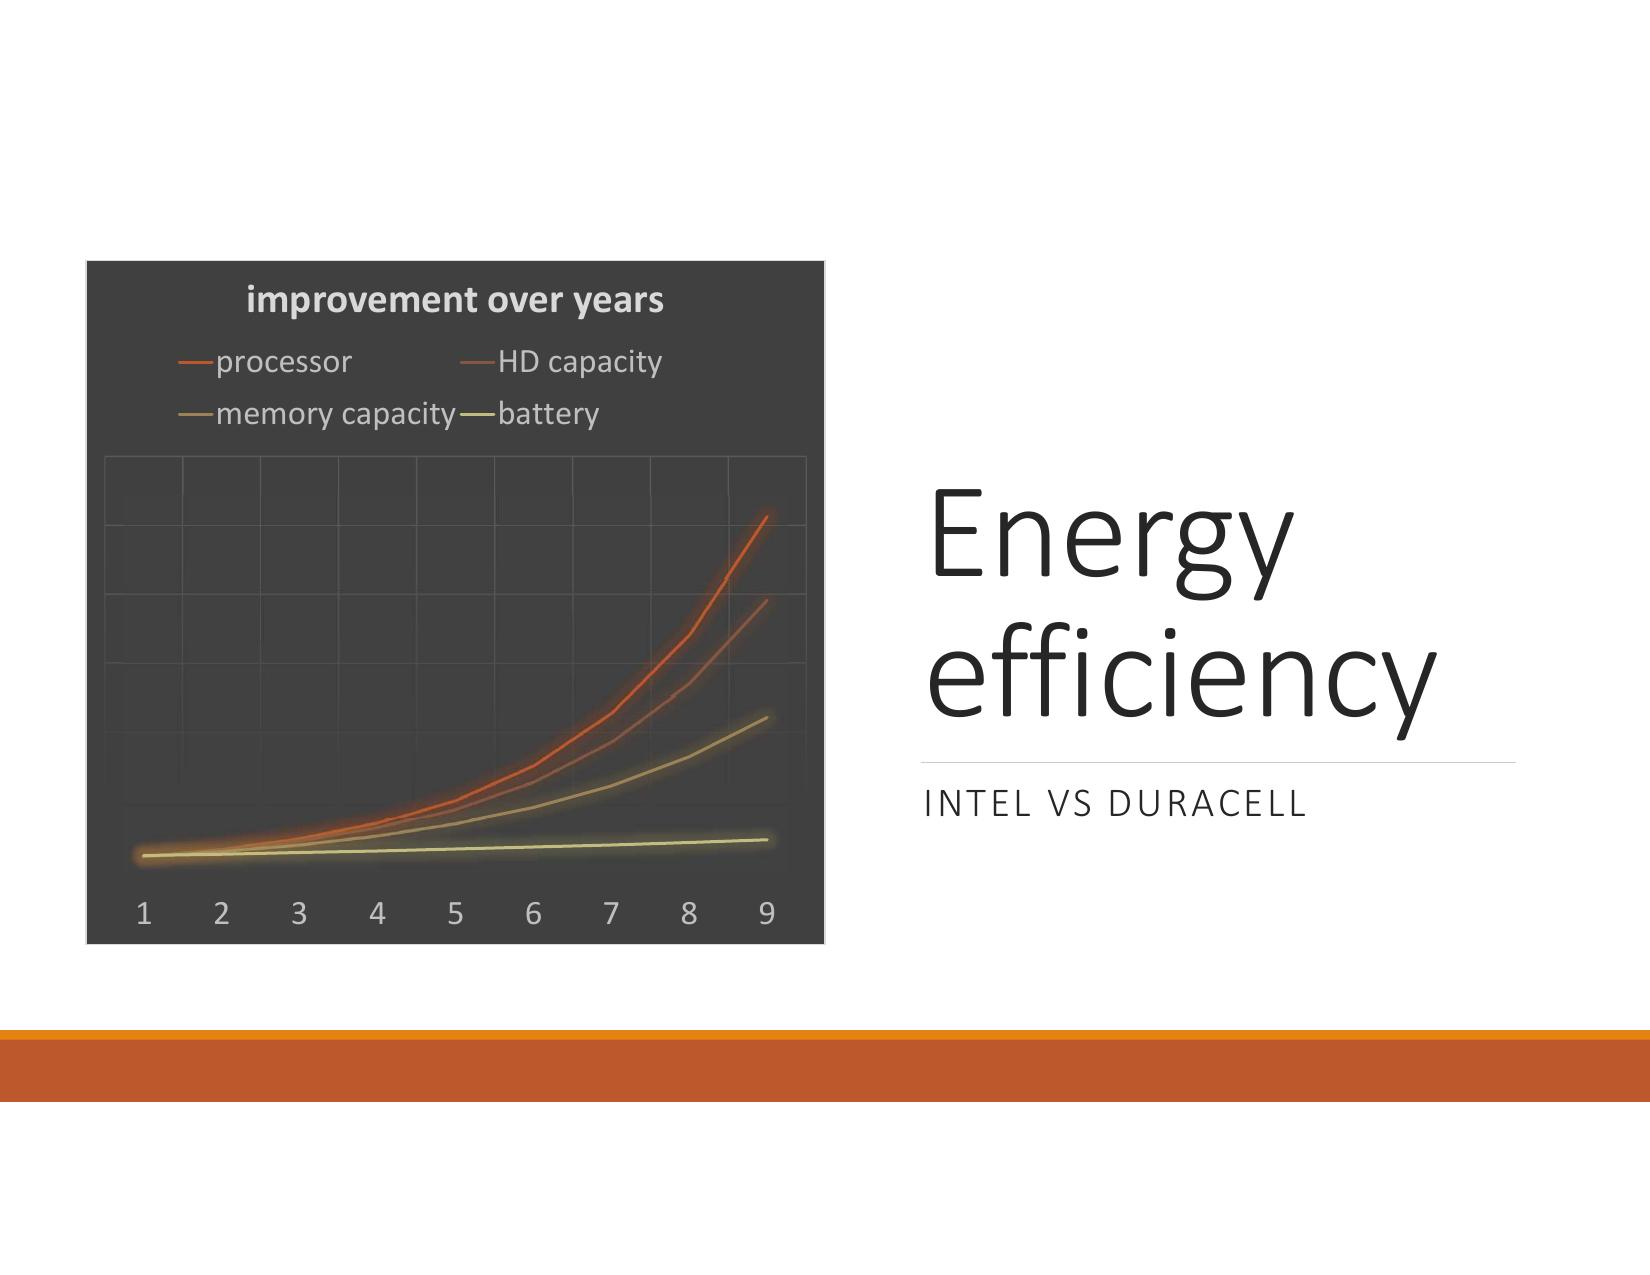
\includegraphics[keepaspectratio]{images/lezione-14-iot-design-img-01.jpg}}
\caption{Il confronto ``Intel vs Duracell'': le curve di processore, HD
e memoria crescono esponenzialmente nel tempo, mentre quella della
batteria rimane quasi orizzontale. Il gap energetico si allarga
progressivamente.}
\end{figure}

Questo significa che più un nodo è capace di fare (più calcolo, più
trasmissioni), più la batteria diventa il collo di bottiglia. Non si può
semplicemente aspettare che le batterie migliorino: bisogna progettare
per consumare meno.

\subsection{Dove va l'energia: laptop vs
sensore}\label{dove-va-lenergia-laptop-vs-sensore}

Per capire dove concentrare gli sforzi di ottimizzazione, è utile
confrontare la distribuzione del consumo energetico in un laptop
(sistema general-purpose) con quella di un sensore wireless.

\begin{figure}
\centering
\pandocbounded{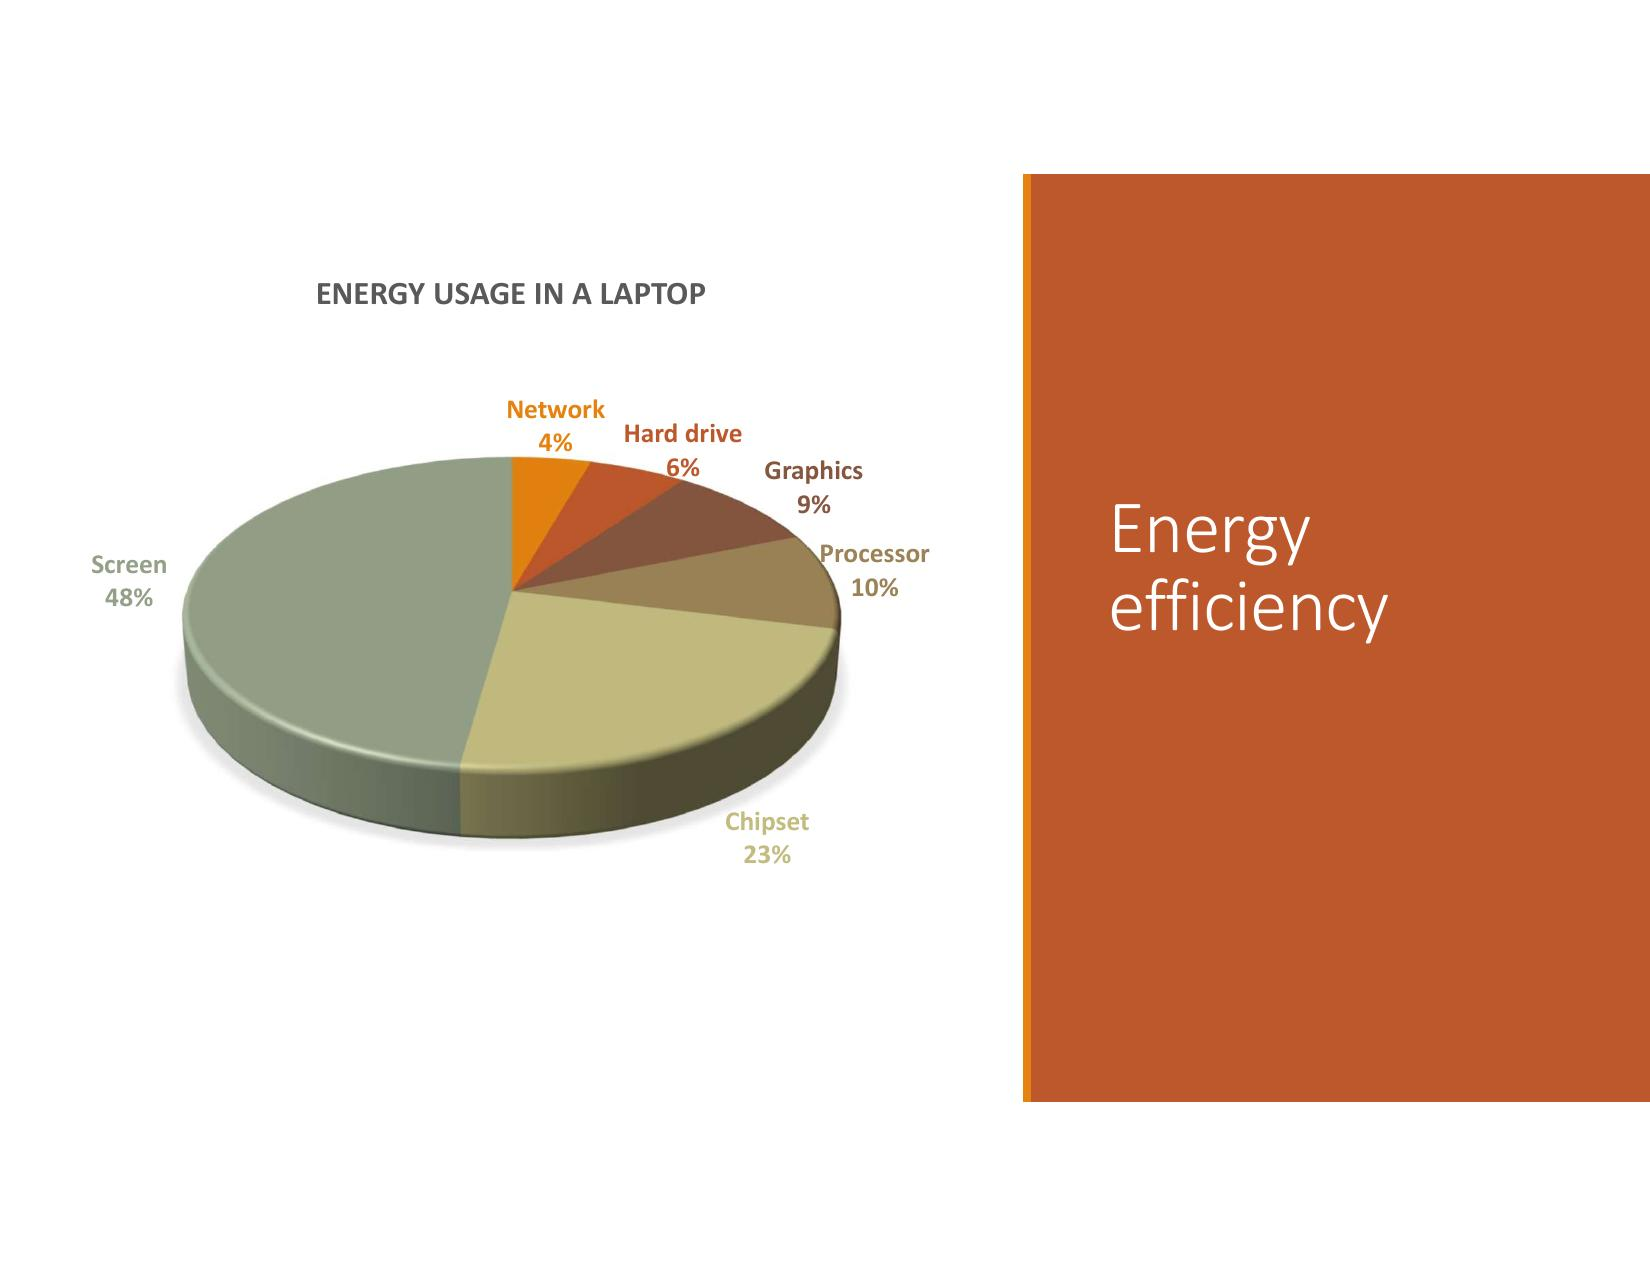
\includegraphics[keepaspectratio]{images/lezione-14-iot-design-img-02.jpg}}
\caption{Ripartizione del consumo energetico in un laptop: lo schermo
domina con il 48\%, seguito dal chipset (23\%), processore (10\%),
grafica (9\%), HD (6\%) e rete (4\%). In un sistema general-purpose lo
schermo è il primo target di ottimizzazione.}
\end{figure}

In un laptop lo \textbf{schermo} assorbe quasi la metà dell'energia
totale (48\%), e le tecniche di risparmio energetico si concentrano su
di esso (backlight dimming, display off automatico). Il processore
incide solo per il 10\%.

\begin{figure}
\centering
\pandocbounded{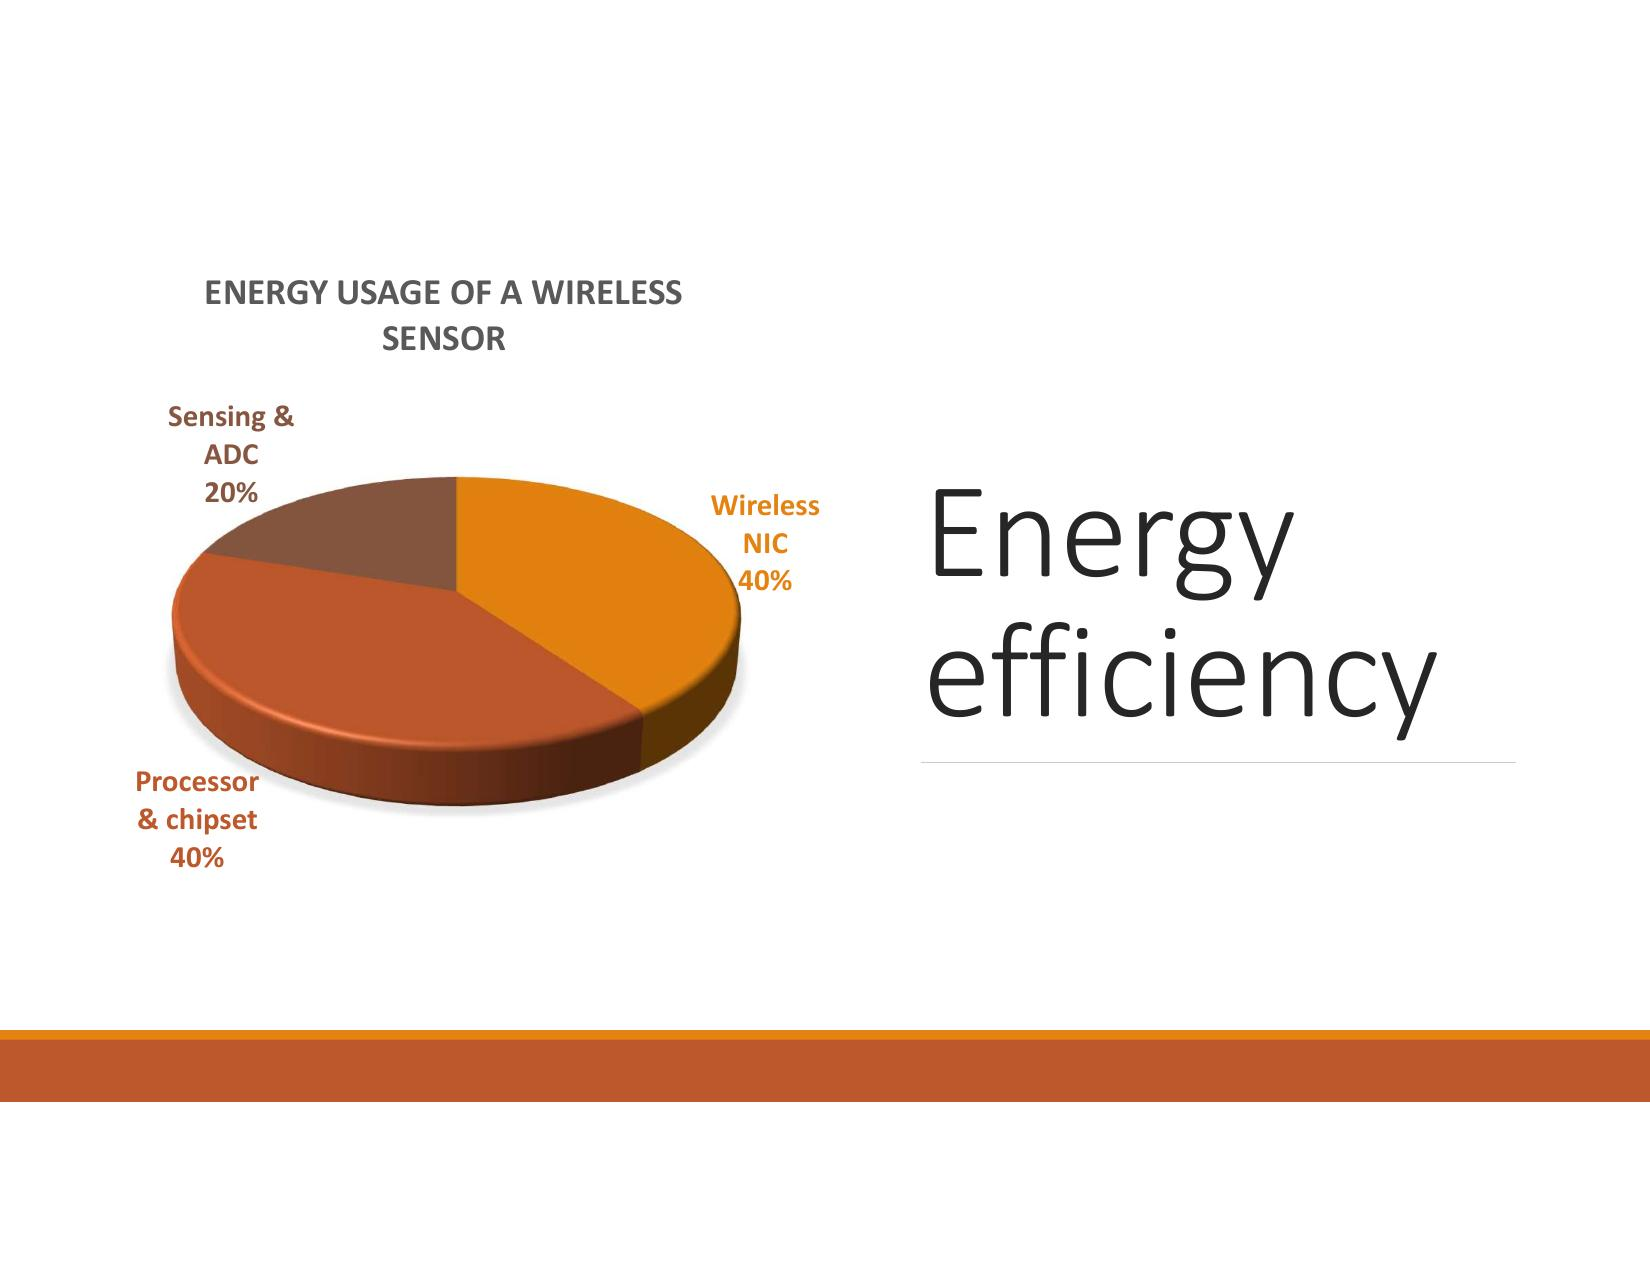
\includegraphics[keepaspectratio]{images/lezione-14-iot-design-img-03.jpg}}
\caption{Ripartizione del consumo energetico in un sensore wireless: il
Wireless NIC e il processore+chipset si equivalgono al 40\% ciascuno,
mentre sensing e ADC pesano il 20\%. Non c'è schermo, quindi la radio
diventa il componente critico.}
\end{figure}

In un sensore wireless lo scenario è radicalmente diverso. \textbf{Non
c'è schermo}. Il consumo è distribuito tra la scheda radio (NIC
wireless, 40\%), il processore e chipset (40\%), e il campionamento con
conversione A/D (20\%). Processore e radio sono i due target principali
per l'ottimizzazione.

\subsection{Consumi della radio: un dettaglio
cruciale}\label{consumi-della-radio-un-dettaglio-cruciale}

Per comprendere perché la radio è così critica, vediamo i consumi di una
tipica interfaccia WiFi:

\begin{itemize}
\tightlist
\item
  \textbf{Sleep mode}: 10 mA
\item
  \textbf{Listen mode} (in ascolto): 180 mA
\item
  \textbf{Receive mode} (ricezione attiva): 200 mA
\item
  \textbf{Transmit mode} (trasmissione): 280 mA
\end{itemize}

Due osservazioni importanti: 1. La differenza tra sleep e listen è
enorme: la radio in ascolto consuma 18 volte più della radio in sleep.
Il semplice fatto di tenere la radio accesa e in ascolto è estremamente
costoso. 2. In alcuni sensori il consumo in trasmissione è
\textbf{inferiore} a quello in ricezione. Questo sembra controintuitivo
ma dipende dai circuiti di amplificazione e dalla specifica
implementazione hardware.

Su un sensore di classe Mote con interfaccia radio a bassa potenza i
valori sono molto più contenuti: sleep a 0,016 mW, ascolto a 12,36 mW,
ricezione a 12,50 mW, trasmissione tra 12,36 mW e 17,76 mW a seconda
della potenza trasmissiva. Si conferma che il costo del ``listen'' è
quasi pari al ``receive'': \textbf{tenere la radio accesa è costoso
anche quando non si trasmette nulla}.

\begin{calloutwarning}{Radio accesa = energia sprecata}

Il consumo in modalità listen è paragonabile a quello in ricezione, e
ordini di grandezza superiore allo sleep. La radio deve essere spenta il
più possibile. Lo stesso vale per il processore: anche il
turn-on/turn-off ha un costo energetico non trascurabile.

\end{calloutwarning}

\begin{center}\rule{0.5\linewidth}{0.5pt}\end{center}

\section{Duty Cycle}\label{duty-cycle}

\subsection{Motivazione: spegnere per
risparmiare}\label{motivazione-spegnere-per-risparmiare}

La soluzione alla sfida energetica si chiama \textbf{duty cycle} (ciclo
di lavoro). L'attività di un nodo IoT è tipicamente ripetitiva: campiona
il sensore, elabora, trasmette, attendi, ricomincia. L'idea è di
sfruttare i periodi di inattività per mettere in sleep tutti i
componenti possibili, riducendo al minimo il consumo.

\begin{calloutdefinition}{Duty Cycle (DC)}

Il duty cycle è la frazione di un periodo in cui il sistema (o un suo
componente) è attivo. Si esprime come rapporto o percentuale: DC =
t\_attivo / T\_periodo. Un DC del 100\% significa sistema sempre attivo;
un DC dell'1\% significa attivo solo l'1\% del tempo.

\end{calloutdefinition}

Il duty cycle ha senso per sistemi che operano in modo \textbf{ciclico}:
eseguono la loro attività periodicamente e rimangono inattivi per la
parte restante del periodo. Applicarlo in modo aggressivo è la leva
principale per estendere la vita della batteria.

\subsection{Esempio pratico: il codice
Arduino}\label{esempio-pratico-il-codice-arduino}

Consideriamo un semplice programma Arduino che legge un sensore
analogico e trasmette il valore via seriale, con una pausa di 380 ms tra
un'iterazione e l'altra. La ripartizione temporale di un singolo ciclo
di 400 ms è:

{\def\LTcaptype{none} % do not increment counter
\begin{longtable}[]{@{}lll@{}}
\toprule\noalign{}
Fase & Durata & Componenti attivi \\
\midrule\noalign{}
\endhead
\bottomrule\noalign{}
\endlastfoot
Campionamento & 4 ms & Processore + Sensore \\
Elaborazione & 1 ms & Solo Processore \\
Trasmissione & 15 ms & Processore + Radio \\
Attesa (\texttt{idle}) & 380 ms & Nessuno (tutti in sleep) \\
\end{longtable}
}

Il codice ottimizzato, che accende e spegne esplicitamente ogni
componente quando non serve, è:

\begin{Shaded}
\begin{Highlighting}[]
\DataTypeTok{void}\NormalTok{ loop}\OperatorTok{()} \OperatorTok{\{}
\NormalTok{    turnOn}\OperatorTok{(}\NormalTok{analogSensor}\OperatorTok{);}
    \DataTypeTok{int}\NormalTok{ sensorValue }\OperatorTok{=}\NormalTok{ analogRead}\OperatorTok{(}\NormalTok{A0}\OperatorTok{);}
\NormalTok{    turnOff}\OperatorTok{(}\NormalTok{analogSensor}\OperatorTok{);}
    
    \DataTypeTok{float}\NormalTok{ voltage }\OperatorTok{=}\NormalTok{ sensorValue }\OperatorTok{*} \OperatorTok{(}\FloatTok{5.0} \OperatorTok{/} \FloatTok{1023.0}\OperatorTok{);}
    
\NormalTok{    turnOn}\OperatorTok{(}\NormalTok{radioInterface}\OperatorTok{);}
\NormalTok{    Serial}\OperatorTok{.}\NormalTok{println}\OperatorTok{(}\NormalTok{voltage}\OperatorTok{);}
\NormalTok{    turnOff}\OperatorTok{(}\NormalTok{radioInterface}\OperatorTok{);}
    
\NormalTok{    idle}\OperatorTok{(}\DecValTok{380}\OperatorTok{);}  \CommentTok{// tutto in sleep per 380 ms}
\OperatorTok{\}}
\end{Highlighting}
\end{Shaded}

Il duty cycle di ciascun componente si calcola come:

\[DC_\text{componente} = \frac{t_\text{attivo}}{T_\text{periodo}}\]

\begin{itemize}
\tightlist
\item
  \textbf{Processore}: attivo per 4+1+15 = 20 ms su 400 ms →
  \(DC_p = 20/400 = 5\%\)
\item
  \textbf{Radio}: attiva per 15 ms su 400 ms →
  \(DC_r = 15/400 = 3,75\%\)
\item
  \textbf{Sensore}: attivo per 4 ms su 400 ms → \(DC_s = 4/400 = 1\%\)
\end{itemize}

Il diagramma energia-tempo chiarisce visivamente questa struttura a
stati:

\begin{figure}
\centering
\pandocbounded{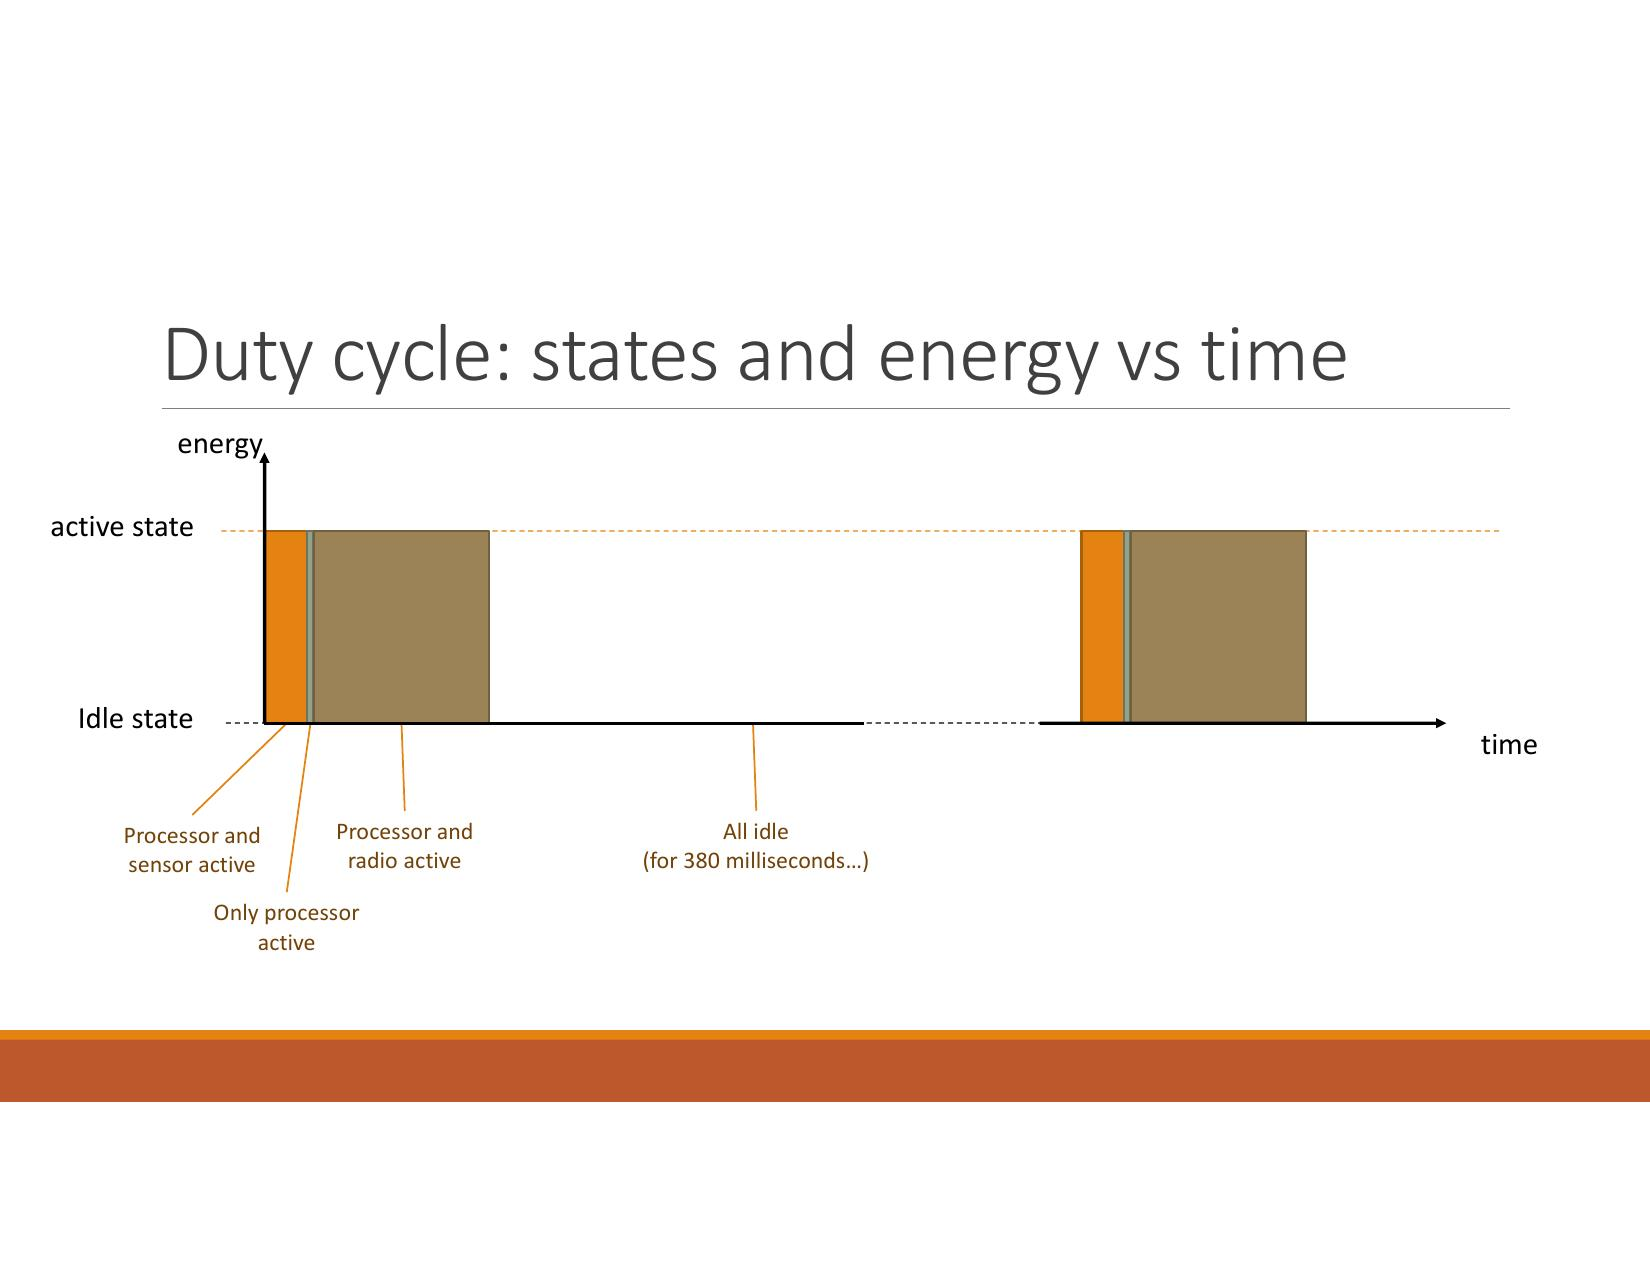
\includegraphics[keepaspectratio]{images/lezione-14-iot-design-img-04.jpg}}
\caption{Diagramma stati/energia vs tempo per il codice di esempio: il
consumo istantaneo varia a scalini in base ai componenti attivi. Il
lungo periodo di idle (380 ms) abbassa drasticamente il consumo medio.}
\end{figure}

\subsection{Calcolo del consumo
energetico}\label{calcolo-del-consumo-energetico}

Il consumo totale di energia di un nodo si calcola sommando i contributi
di ciascun componente. Per un componente generico con duty cycle \(dc\)
il costo energetico per unità di tempo è:

\[E_\text{componente} = dc \cdot C_\text{active} + (1 - dc) \cdot C_\text{idle}\]

dove \(C_\text{active}\) e \(C_\text{idle}\) sono i correnti (in mA)
rispettivamente in stato attivo e in sleep. Poiché si usa corrente
continua e la tensione è (quasi) costante, si può esprimere tutto in
\textbf{mAh} --- sia l'energia consumata che la carica immagazzinata
nella batteria.

Per il microprocessore il costo per ciclo è:

\[E_\mu = C_\mu^{full} \cdot dc_\mu + C_\mu^{idle} \cdot (1 - dc_\mu)\]

Per la radio, che ha due stati attivi (trasmissione e ricezione):

\[E_\rho = C_\rho^T \cdot dc_\rho^T + C_\rho^R \cdot dc_\rho^R + C_\rho^{idle} \cdot (1 - dc_\rho^T - dc_\rho^R)\]

Il costo totale per ciclo è la somma di tutti i componenti:

\[E = E_\mu + E_\rho + E_\lambda + E_\sigma\]

dove \(E_\lambda\) è il costo del logger (memoria flash) e \(E_\sigma\)
quello della scheda sensori.

\subsection{Calcolo del lifetime}\label{calcolo-del-lifetime}

La vita utile del dispositivo dipende da quanta energia ha a
disposizione (capacità della batteria \(B_0\)) e da quanto ne consuma
per ciclo (\(E\)). Ignorando la perdita di carica della batteria per
autoscarica, il lifetime in numero di cicli è:

\[Lifetime = \frac{B_0}{E}\]

Se si tiene conto dell'autoscarica della batteria (perdita percentuale
\(\varepsilon\) per ciclo), la carica residua segue la ricorrenza:

\[B_n = B_{n-1} \cdot (1 - \varepsilon) - E\]

Risolvendo la ricorrenza si ottiene:

\[B_n = B_0 \cdot (1-\varepsilon)^{n-1} + \frac{E \cdot ((1-\varepsilon)^n - 1)}{\varepsilon}\]

Il lifetime in cicli è il valore di \(n\) per cui \(B_n = 0\). In
pratica il dispositivo smette di funzionare prima, quando la tensione
scende sotto una soglia minima.

\subsection{Effetto del duty cycle sulla vita della
batteria}\label{effetto-del-duty-cycle-sulla-vita-della-batteria}

I due grafici seguenti mostrano empiricamente l'impatto del duty cycle
sulla vita di un nodo basato su specifiche hardware reali (Mote-class):

\begin{figure}
\centering
\pandocbounded{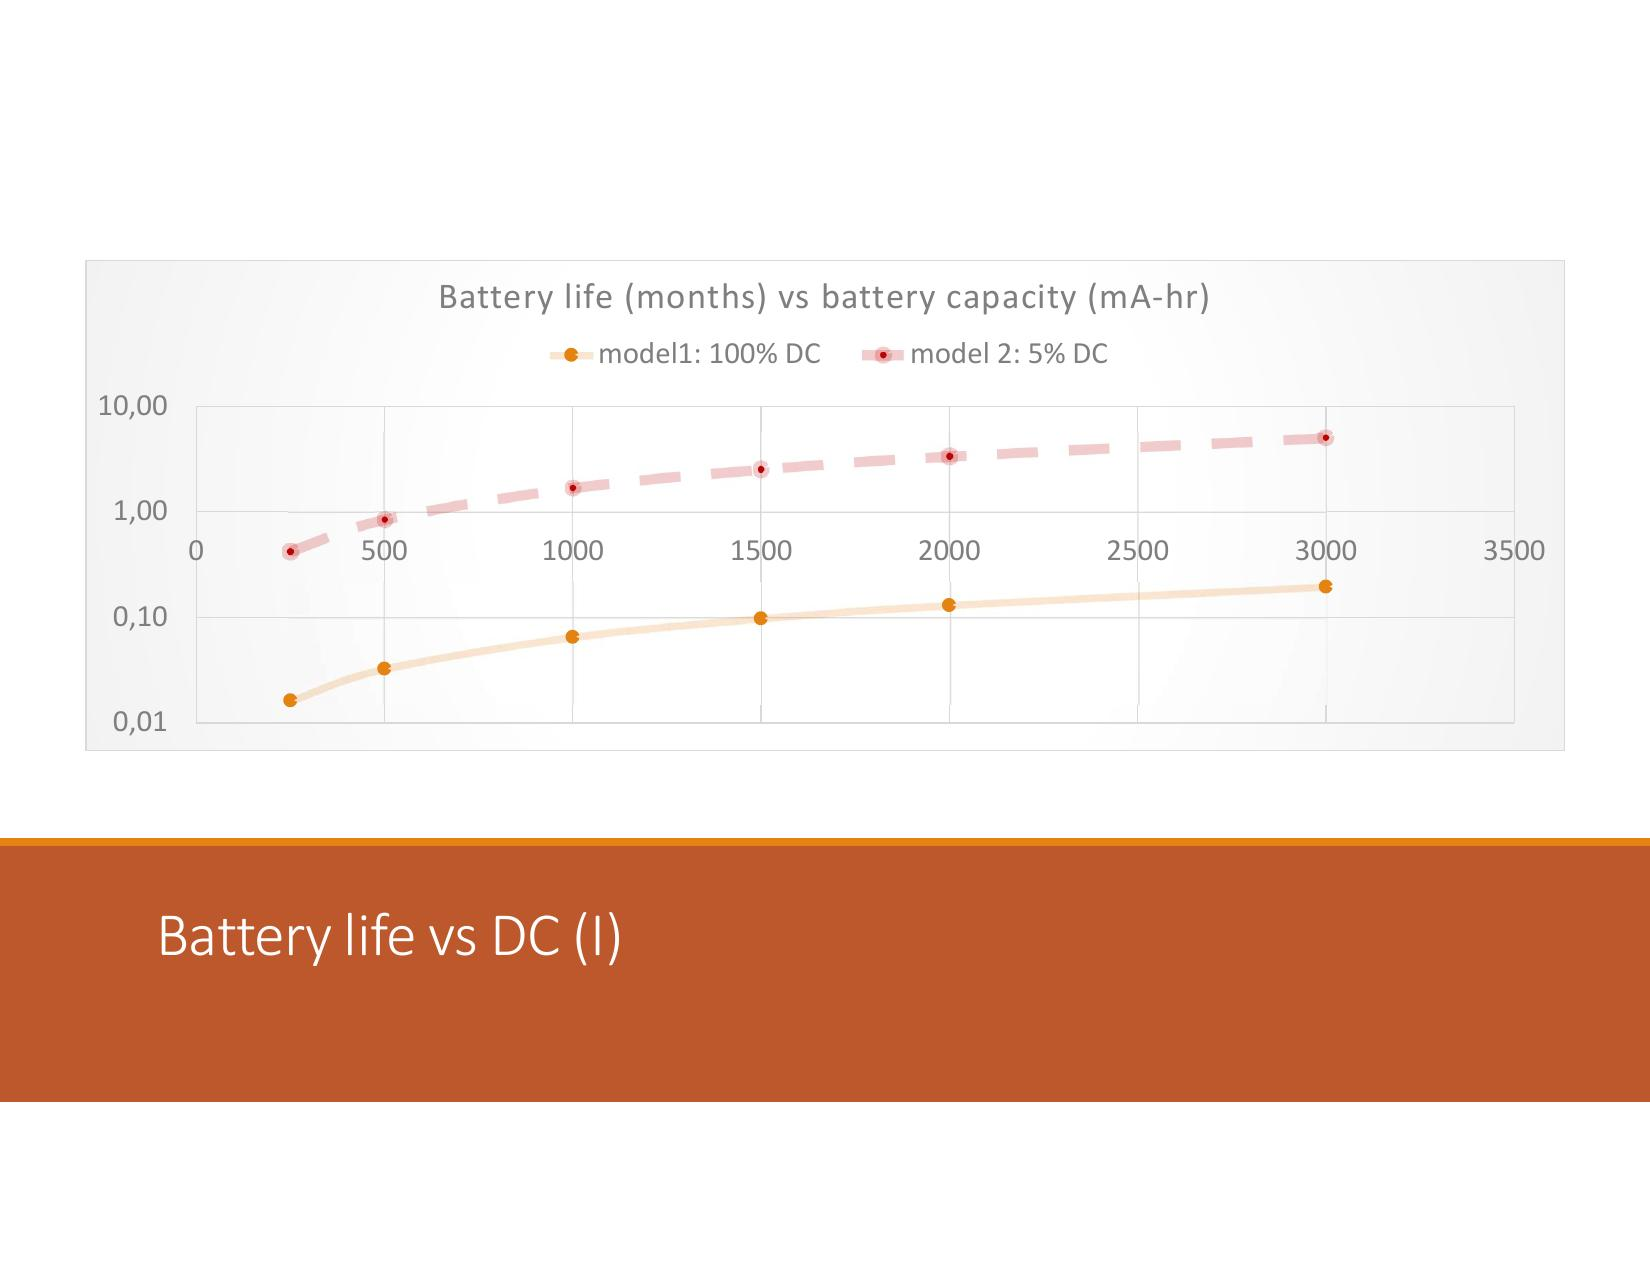
\includegraphics[keepaspectratio]{images/lezione-14-iot-design-img-05.jpg}}
\caption{Vita della batteria in mesi vs capacità (mA-hr) per due
modelli: DC al 100\% e DC al 5\%. Scala logaritmica sull'asse Y. A
parità di capacità, il modello con DC al 5\% ha una vita circa 10-15
volte superiore.}
\end{figure}

\begin{figure}
\centering
\pandocbounded{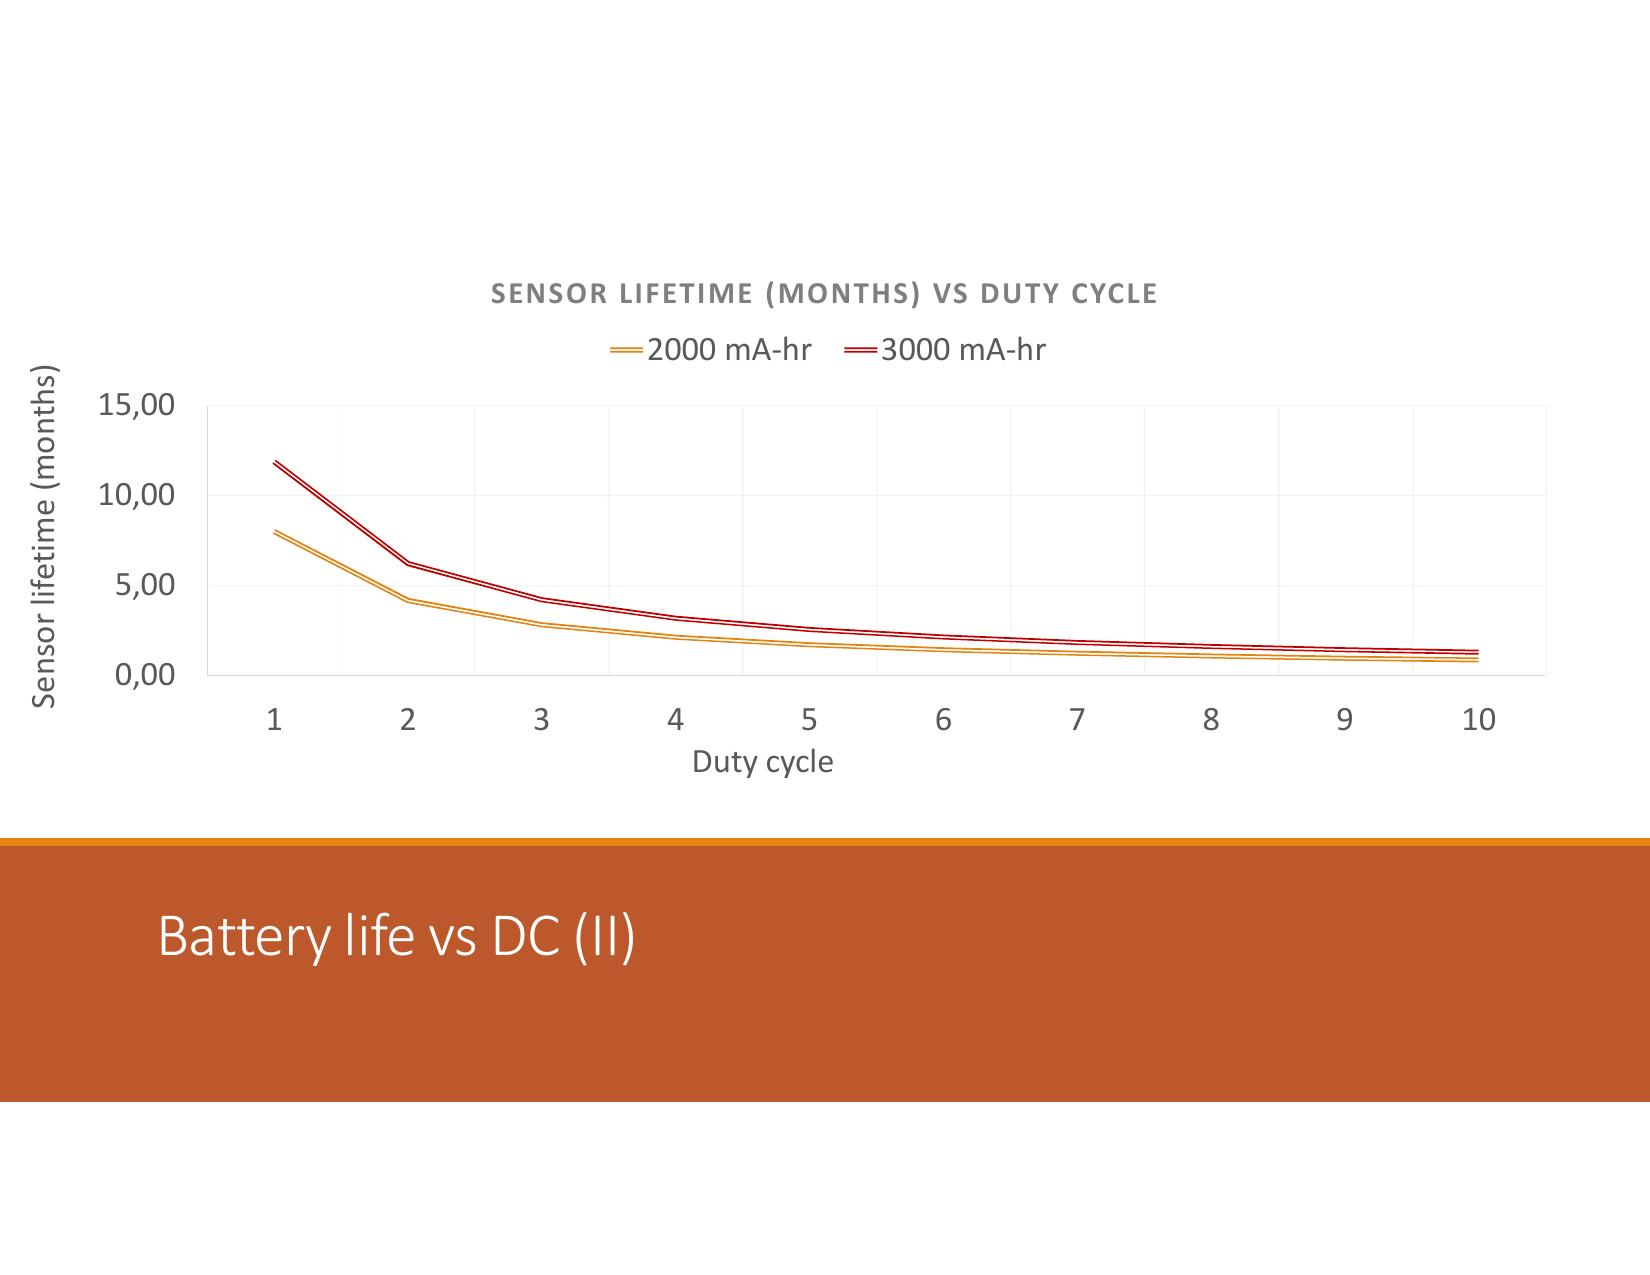
\includegraphics[keepaspectratio]{images/lezione-14-iot-design-img-06.jpg}}
\caption{Vita del sensore (mesi) vs duty cycle per batterie da 2000 e
3000 mA-hr. La curva scende rapidamente: già passare dall'1\% al 3\% di
DC dimezza approssimativamente il lifetime. L'effetto della capacità
della batteria diventa trascurabile ad alti DC.}
\end{figure}

Questi grafici mostrano due cose fondamentali. Prima cosa: ridurre il
duty cycle è molto più efficace che aumentare la capacità della batteria
--- a DC alto le due curve per 2000 e 3000 mAh si sovrappongono, segno
che la batteria più grande non aiuta quasi più. Seconda cosa: anche un
DC basso ma non zero (5\%) porta a lifetime dell'ordine dei mesi, non
degli anni. Per applicazioni con deployment di lunga durata è necessario
DC molto bassi o {[}{[}Energy Harvesting{]}{]}.

\subsection{Esempio numerico: soluzione dell'esercizio
base}\label{esempio-numerico-soluzione-dellesercizio-base}

Con le specifiche della Mote (ATmega128L: 8 mA full, 15 μA sleep; Radio:
20 mA xmit, 20 μA sleep; Sensor Board: 5 mA full, 5 μA sleep; Batteria:
2000 mAh) e il codice di esempio (periodo 400 ms, sensore 4 ms, calcolo
1 ms, trasmissione 15 ms, idle 380 ms):

\begin{itemize}
\tightlist
\item
  \(dc_p = 5\%\), \(dc_r = 3,75\%\), \(dc_s = 1\%\)
\end{itemize}

Il consumo per ora risulta 1,243 mAh, ripartito tra:

{\def\LTcaptype{none} % do not increment counter
\begin{longtable}[]{@{}lll@{}}
\toprule\noalign{}
Componente & Contributo idle & Contributo attivo \\
\midrule\noalign{}
\endhead
\bottomrule\noalign{}
\endlastfoot
Processore & 0,014 mAh & 0,4 mAh \\
Radio & 0,019 mAh & 0,75 mAh \\
Sensore & 0,005 mAh & 0,055 mAh \\
\textbf{Totale} & 0,038 mAh & 1,205 mAh \\
\end{longtable}
}

\textbf{Lifetime ≈ 2000 / 1,243 ≈ 1609 ore} (circa 67 giorni).

\subsection{La complessità nascosta: spegnere la radio è una decisione
globale}\label{la-complessituxe0-nascosta-spegnere-la-radio-uxe8-una-decisione-globale}

Spegnere il processore è una scelta locale: lo scheduler del nodo sa
quando il processore non serve e può metterlo in sleep autonomamente.
Spegnere la radio è invece una \textbf{decisione globale}: un nodo con
radio spenta non può ricevere messaggi, non può fungere da router in una
rete multi-hop, non può ricevere comandi o aggiornamenti. Un'intera rete
di nodi che si addormentano nello stesso momento sarebbe inutile.

Questo crea un trade-off fondamentale: più i nodi dormono, meno
consumano, ma peggiore è la capacità di comunicare. La soluzione sta nei
\textbf{protocolli MAC} (Medium Access Control) progettati per l'IoT,
che sincronizzano i nodi e coordinano chi può dormire e quando. Questi
protocolli implementano strategie di risparmio energetico a livello di
rete, e saranno oggetto delle lezioni successive.

\begin{center}\rule{0.5\linewidth}{0.5pt}\end{center}

\section{Esercizi: Calcolo di DC e
Lifetime}\label{esercizi-calcolo-di-dc-e-lifetime}

\subsection{Esercizio 1 --- Monitoraggio Frequenza Cardiaca (invio
raw)}\label{esercizio-1-monitoraggio-frequenza-cardiaca-invio-raw}

In questo scenario un dispositivo campiona un fotodiodo sul polso a 20
Hz (campionamento da 0,5 ms, richiede processore + sensore attivi), e
invia ogni 5 campioni consecutivi al server (trasmissione da 2 ms ogni
0,25 s, richiede processore + radio). Il calcolo HR è demandato al
server.

\begin{itemize}
\tightlist
\item
  \(dc_\text{sampling} = 0,5\,ms / 50\,ms = 0,01\) (1\%)
\item
  \(dc_\text{radio} = 2\,ms / 250\,ms = 0,008\) (0,8\%)
\item
  \(dc_\text{processor} = dc_\text{sampling} + dc_\text{radio} = 0,018\)
  (1,8\%)
\end{itemize}

Consumo per ora: 0,3935 mAh → \textbf{Lifetime ≈ 5082 ore
(\textasciitilde212 giorni)}.

\subsection{Esercizio 2 --- Monitoraggio HR con calcolo
in-device}\label{esercizio-2-monitoraggio-hr-con-calcolo-in-device}

In questo scenario il dispositivo calcola HR localmente (ogni 2 s,
elaborazione da 5 ms, solo processore) e trasmette solo 1 pacchetto ogni
10 s (2 ms di trasmissione).

\begin{itemize}
\tightlist
\item
  \(dc_\text{sampling} = 0,01\) (identico al caso precedente)
\item
  \(dc_\text{processing} = 5\,ms / 2000\,ms = 0,0025\)
\item
  \(dc_\text{radio} = 2\,ms / 10000\,ms = 0,0002\)
\item
  \(dc_\text{processor} = 0,01 + 0,0025 + 0,0002 = 0,0127\)
\end{itemize}

Consumo per ora: 0,1954 mAh → \textbf{Lifetime ≈ 10.235 ore
(\textasciitilde426 giorni)}.

\begin{callouttip}{Edge processing vs cloud offloading}

Il confronto tra i due esercizi rivela un principio fondamentale
nell'IoT: elaborare i dati in-loco (\textbf{edge processing}) invece di
inviare tutti i campioni grezzi al server può ridurre drasticamente le
trasmissioni radio --- il componente più energivoro dopo il processore.
Nonostante il calcolo HR aggiunga un piccolo overhead al processore, il
risparmio sulla radio più che compensa, raddoppiando circa il lifetime.

\end{callouttip}

\begin{center}\rule{0.5\linewidth}{0.5pt}\end{center}

\section{Conclusioni e Punti Chiave}\label{conclusioni-e-punti-chiave}

La lezione ha costruito un quadro coerente intorno al problema
energetico nell'IoT. I vincoli di processing, memoria, batteria e
comunicazione non saranno risolti automaticamente dalla Legge di Moore,
che nell'IoT viene usata principalmente per ridurre costi e dimensioni
piuttosto che per aumentare le prestazioni. La sfida energetica persiste
perché la capacità delle batterie non cresce al ritmo dei transistor.

L'efficienza energetica si ottiene comprendendo dove va l'energia (radio
e processore sono i componenti dominanti, non lo schermo come nel
laptop) e applicando il duty cycle per spegnere ogni componente quando
non è necessario. Il modello formale permette di calcolare con
precisione il consumo per ciclo e il lifetime atteso. La prossima
lezione approfondirà i protocolli MAC per l'IoT, che risolvono il
problema della coordinazione del duty cycle a livello di rete.

\newpage

\chapter{Protocolli MAC per Reti Wireless
Multi-hop}\label{protocolli-mac-per-reti-wireless-multi-hop}

\section{Il problema dell'efficienza
energetica}\label{il-problema-dellefficienza-energetica}

Nei sistemi IoT e nelle reti di sensori wireless, il protocollo MAC non
ha come unico obiettivo l'arbitrazione dell'accesso al mezzo: deve anche
--- e soprattutto --- minimizzare il consumo energetico dei nodi. La
ragione è semplice: i dispositivi sono tipicamente alimentati a batteria
e devono operare per mesi o anni senza manutenzione. Il radio
transceiver è di gran lunga il componente più energivoro, e la strategia
fondamentale è ridurne il \textbf{duty cycle}, ovvero la frazione di
tempo in cui rimane attivo.

\begin{callouttip}{Intuizione chiave}

Un nodo con la radio sempre accesa è connesso ma scarica la batteria
rapidamente. Un nodo con la radio sempre spenta risparmia energia ma non
può comunicare. Il protocollo MAC deve trovare il giusto compromesso.

\end{callouttip}

Il tradeoff principale è tra \textbf{energia} da un lato e
\textbf{latenza e banda} dall'altro: abbassare il duty cycle risparmia
energia ma aumenta il tempo di attesa prima che i pacchetti possano
essere trasmessi o ricevuti.

Esistono tre approcci fondamentali per ridurre il consumo:

{\def\LTcaptype{none} % do not increment counter
\begin{longtable}[]{@{}
  >{\raggedright\arraybackslash}p{(\linewidth - 4\tabcolsep) * \real{0.3333}}
  >{\raggedright\arraybackslash}p{(\linewidth - 4\tabcolsep) * \real{0.3333}}
  >{\raggedright\arraybackslash}p{(\linewidth - 4\tabcolsep) * \real{0.3333}}@{}}
\toprule\noalign{}
\begin{minipage}[b]{\linewidth}\raggedright
Approccio
\end{minipage} & \begin{minipage}[b]{\linewidth}\raggedright
Descrizione
\end{minipage} & \begin{minipage}[b]{\linewidth}\raggedright
Esempi
\end{minipage} \\
\midrule\noalign{}
\endhead
\bottomrule\noalign{}
\endlastfoot
Sincronizzazione dei nodi & I nodi si svegliano contemporaneamente per
comunicare & S-MAC, IEEE 802.15.4 \\
Preamble sampling & Il mittente invia un lungo preambolo; il ricevitore
campiona periodicamente il canale & B-MAC, X-MAC, BoX-MAC \\
Polling & Un master coordina i nodi slave tramite beacon periodici &
Bluetooth, IEEE 802.15.4 \\
\end{longtable}
}

\begin{center}\rule{0.5\linewidth}{0.5pt}\end{center}

\section{Sincronizzazione: S-MAC}\label{sincronizzazione-s-mac}

S-MAC (\emph{Sensor MAC}) è un protocollo progettato per reti wireless
multi-hop, disponibile in TinyOS per piattaforme come le mica motes
(Iris, Tmote). La sua idea di base è che se i nodi vicini si svegliano
nello stesso istante, possono comunicare durante la finestra di attività
e poi tornare in stato di sleep, riducendo drasticamente il consumo
complessivo.

\begin{calloutdefinition}{Duty cycle in S-MAC}

Ogni nodo alterna periodi di \textbf{listen} (radio accesa, pronto a
ricevere) e periodi di \textbf{sleep} (radio spenta). La finestra di
ascolto è periodica e relativamente breve rispetto al periodo totale.

\end{calloutdefinition}

\subsection{Organizzazione della
sincronizzazione}\label{organizzazione-della-sincronizzazione}

S-MAC non impone una sincronizzazione globale, ma solo \textbf{locale}:
nodi adiacenti si accordano su un periodo di ascolto condiviso. Il
meccanismo è il seguente:

\begin{itemize}
\tightlist
\item
  Ogni nodo trasmette periodicamente dei \textbf{frame SYNC} in
  broadcast, che annunciano la propria schedule (quando si sveglia,
  quando dorme).
\item
  Un nodo che si avvia ascolta il canale per individuare frame SYNC dei
  vicini. Se trova vicini con una schedule già definita, la adotta. In
  caso contrario, sceglie autonomamente la propria schedule e la
  pubblicizza.
\item
  Un nodo può successivamente cambiare la propria schedule se la maggior
  parte dei vicini ha adottato un'altra.
\end{itemize}

Questo approccio consente a sottoreti di adottare schedule diverse,
creando delle \textbf{isole di sincronizzazione} locali. Il risultato
non è una sincronizzazione globale uniforme, ma va bene per la maggior
parte delle topologie pratiche.

\subsection{Comunicazione durante il periodo di
ascolto}\label{comunicazione-durante-il-periodo-di-ascolto}

Un nodo può inviare un frame a un vicino solo durante il \textbf{periodo
di ascolto del ricevitore}, non necessariamente durante il proprio. Ciò
implica che il mittente deve conoscere le schedule di tutti i suoi
vicini e tenere la radio accesa anche al di fuori del proprio periodo di
ascolto quando deve trasmettere.

\begin{calloutnote}{Carrier sense e RTS/CTS}

Prima della trasmissione S-MAC esegue il \textbf{carrier sense}: se il
canale è occupato, il frame viene posticipato al periodo di ascolto
successivo. Per evitare collisioni usa RTS/CTS (come IEEE 802.11). Una
piccola ottimizzazione chiamata \emph{adaptive duty cycle}: se un nodo
riceve un RTS o un CTS in sorveglianza, mantiene la radio accesa fino al
termine della trasmissione, perché potrebbe essere il prossimo hop.

\end{calloutnote}

\begin{figure}
\centering
\pandocbounded{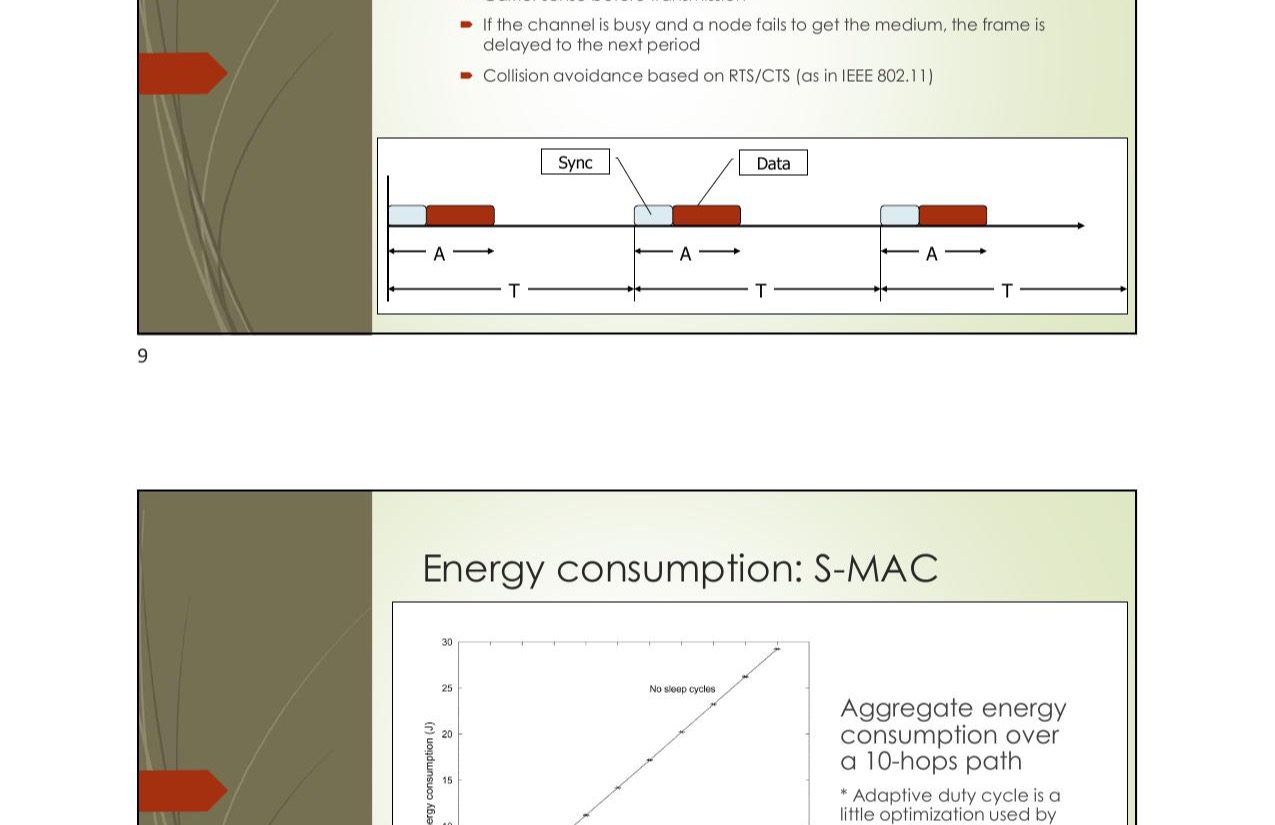
\includegraphics[keepaspectratio]{images/lezione-17-mac-protocols-img-01.jpg}}
\caption{Il frame Sync e il frame Data vengono trasmessi durante il
periodo di attività del ricevitore; i periodi di silenzio T separano le
finestre di ascolto.}
\end{figure}

\begin{figure}
\centering
\pandocbounded{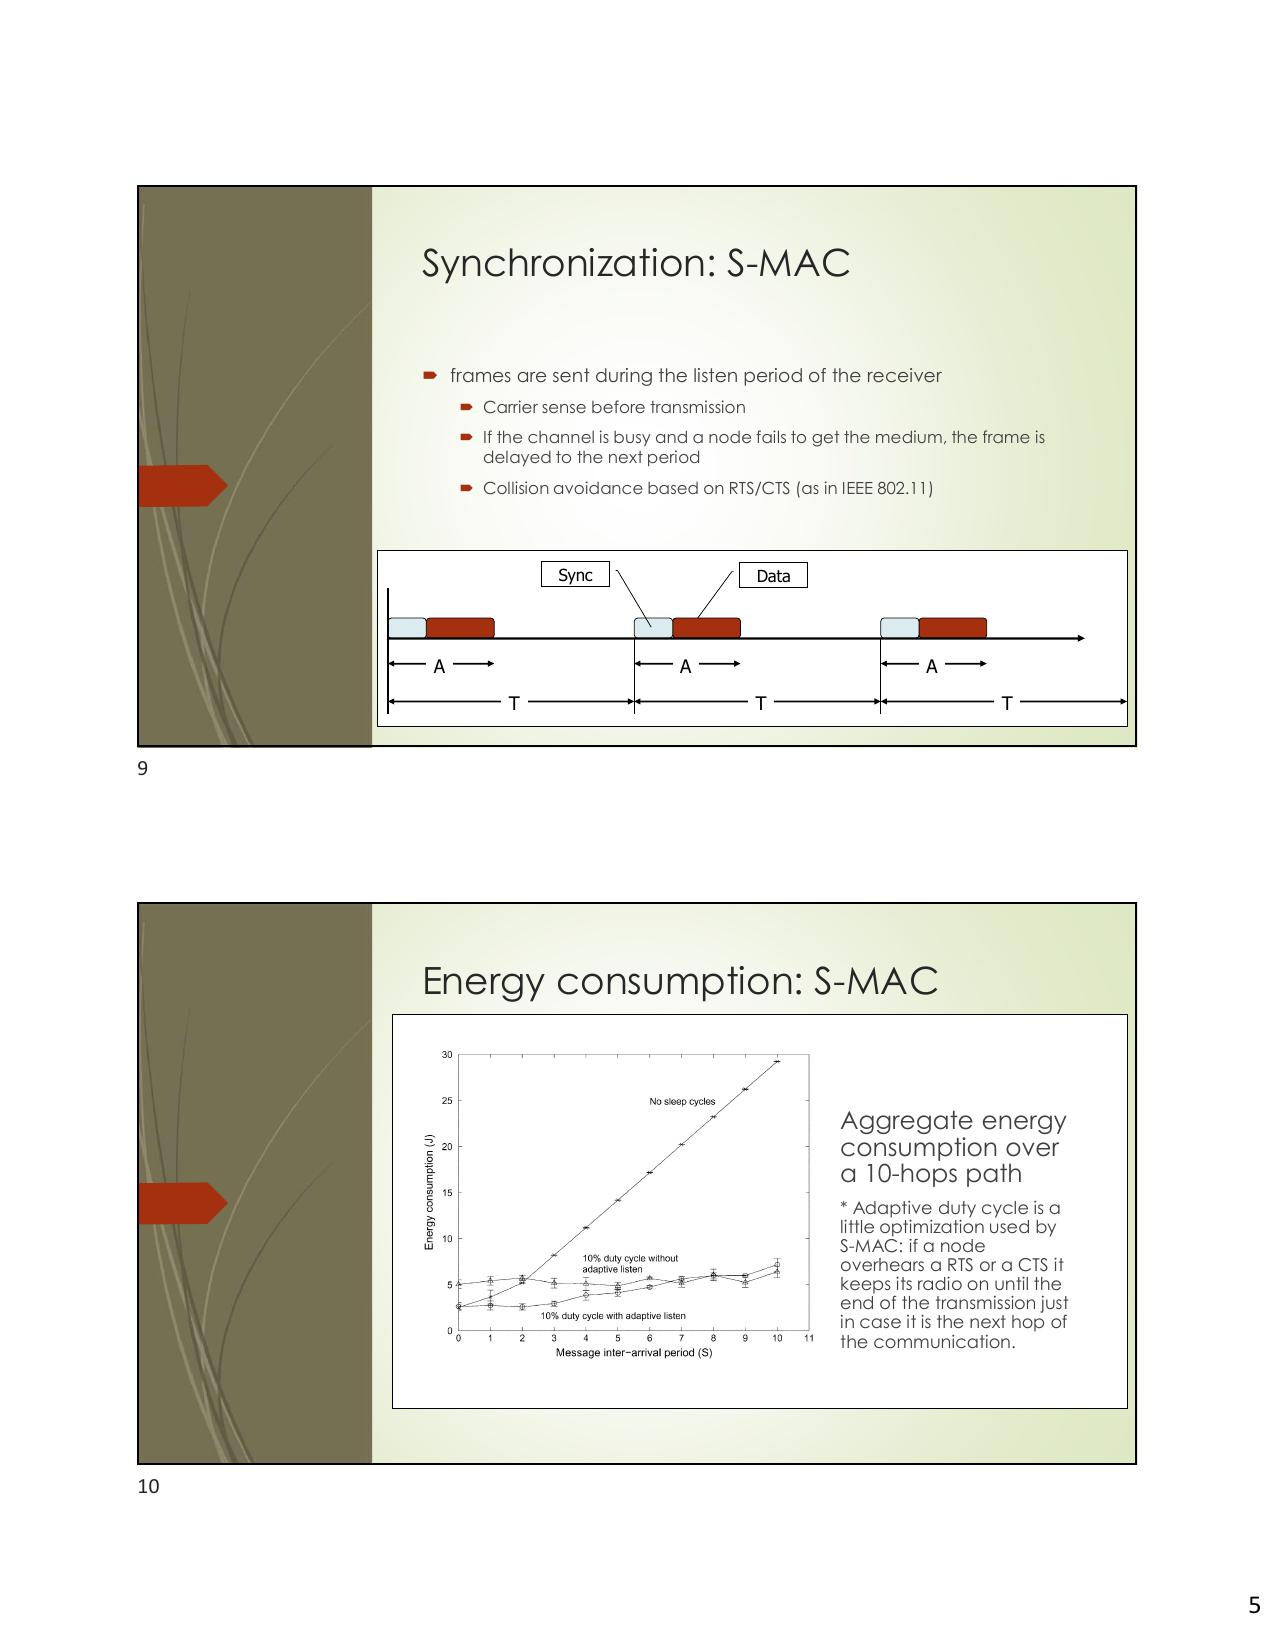
\includegraphics[keepaspectratio]{images/lezione-17-mac-protocols-img-02.jpg}}
\caption{Consumo energetico totale in funzione del periodo inter-arrivo
dei messaggi. La curva ``No sleep cycles'' è il riferimento; il duty
cycle al 10\% riduce drasticamente i consumi; l'adaptive duty cycle
ottimizza ulteriormente.}
\end{figure}

\subsection{Latenza nei percorsi
multi-hop}\label{latenza-nei-percorsi-multi-hop}

La latenza è il tallone d'Achille di S-MAC. In un percorso multi-hop, un
frame deve attraversare una sequenza di nodi intermedi: in ogni hop, nel
caso peggiore, il frame deve attendere fino al successivo periodo di
ascolto del nodo successivo. Se i nodi lungo il percorso hanno schedule
diverse, questo attesa si accumula ad ogni salto.

\begin{calloutwarning}{Latenza nel worst case}

In una catena di \(n\) hop con schedule non allineate, la latenza totale
è proporzionale a \(n \times T_{listen\_period}\). Con duty cycle bassi
(periodo lungo), la latenza può diventare inaccettabile per applicazioni
real-time.

\end{calloutwarning}

Questa latenza è mitigata --- ma non eliminata --- dalla tendenza dei
nodi a convergere verso schedule condivise nel loro vicinato. Se nodi
consecutivi lungo un percorso di routing condividono la stessa schedule,
il frame non deve attendere tra un hop e l'altro. Tuttavia, questo
allineamento non è garantito.

\begin{figure}
\centering
\pandocbounded{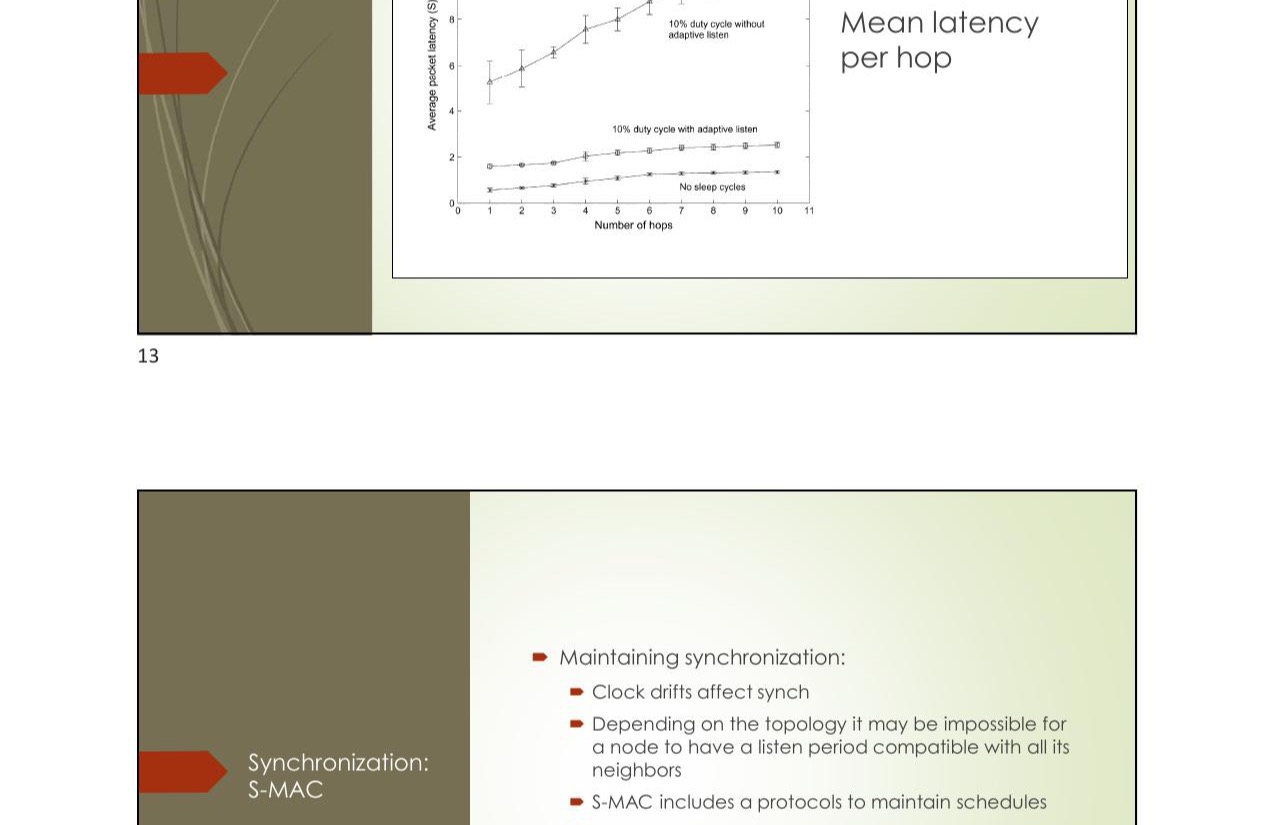
\includegraphics[keepaspectratio]{images/lezione-17-mac-protocols-img-03.jpg}}
\caption{Latenza media per hop in funzione del numero di hop. Il duty
cycle al 10\% senza adaptive listen introduce latenze molto più elevate
rispetto alla modalità senza sleep e alla variante con adaptive listen.}
\end{figure}

\subsection{Mantenimento della
sincronizzazione}\label{mantenimento-della-sincronizzazione}

Nel tempo, il \textbf{clock drift} (deriva dell'orologio hardware) può
desincronizzare i nodi. S-MAC include un meccanismo per il mantenimento
della sincronizzazione basato sui frame SYNC periodici. Inoltre, in
topologie complesse, potrebbe essere impossibile per un nodo avere un
periodo di ascolto compatibile con \emph{tutti} i suoi vicini
simultaneamente, e in quel caso S-MAC permette al nodo di cambiare
schedule o di mantenerne più di una.

\begin{center}\rule{0.5\linewidth}{0.5pt}\end{center}

\section{Preamble Sampling: B-MAC}\label{preamble-sampling-b-mac}

B-MAC (\emph{Berkeley MAC}) rappresenta un approccio radicalmente
diverso: invece di sincronizzare i nodi, \textbf{elimina del tutto la
necessità di coordinazione temporale}. È disponibile in TinyOS per mica
motes e si basa sul concetto di \emph{Low-Power Listening} (LPL).

\begin{calloutdefinition}{Low-Power Listening (LPL)}

Il ricevitore attiva periodicamente la radio per un brevissimo
intervallo e controlla se c'è un preambolo sul canale. Se non rileva
nulla, torna immediatamente in sleep. Se rileva un preambolo, mantiene
la radio accesa per ricevere il frame.

\end{calloutdefinition}

Il mittente, dal canto suo, non deve aspettare il momento giusto:
\textbf{trasmette quando vuole}, ma antepone al frame un
\textbf{preambolo molto lungo} --- più lungo dell'intervallo di sleep
del ricevitore. In questo modo, qualunque sia il momento in cui il
ricevitore esegue il campionamento (preamble sampling), il preambolo è
ancora ``in aria'' e può essere rilevato.

\begin{figure}
\centering
\pandocbounded{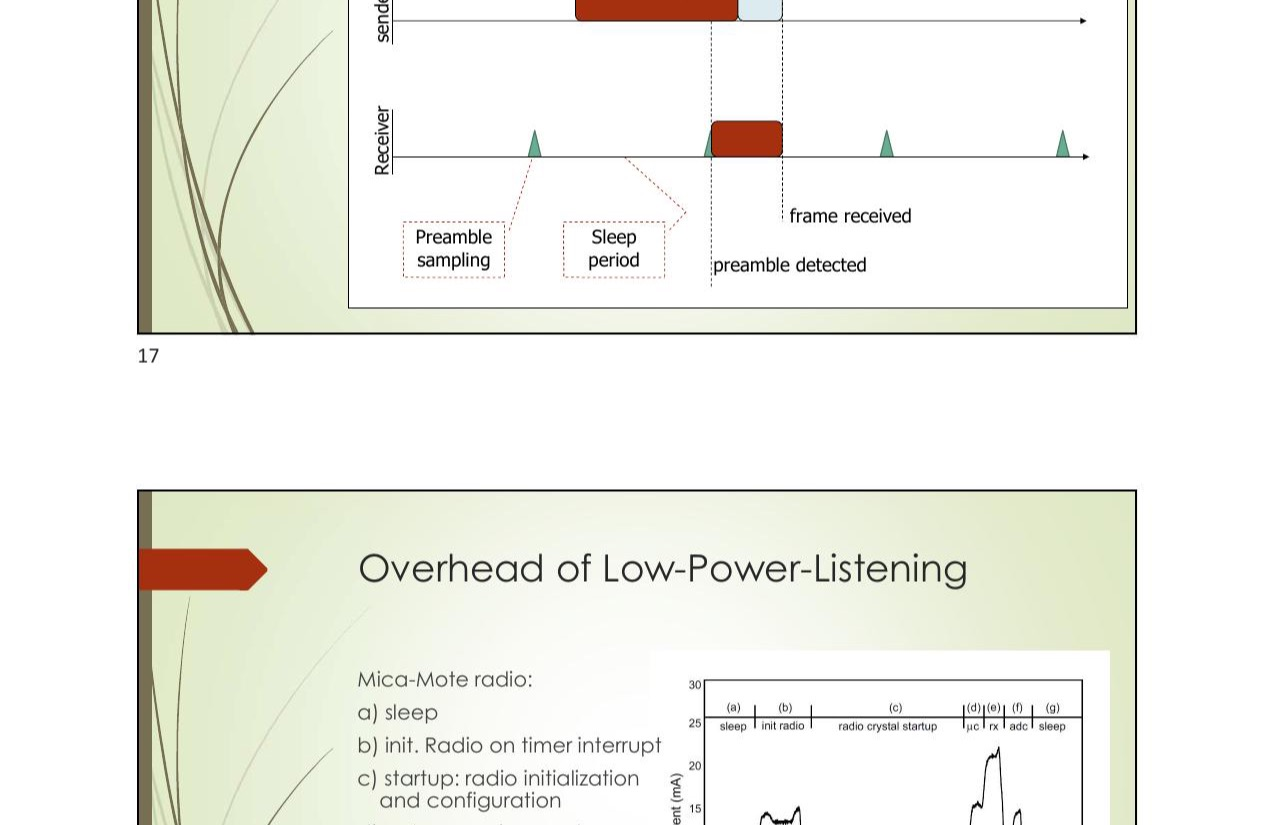
\includegraphics[keepaspectratio]{images/lezione-17-mac-protocols-img-04.jpg}}
\caption{Il mittente trasmette un lungo preambolo seguito dal frame. Il
ricevitore esegue campionamenti brevi e periodici (preamble sampling);
quando rileva il preambolo, mantiene la radio accesa per ricevere il
frame.}
\end{figure}

\begin{figure}
\centering
\pandocbounded{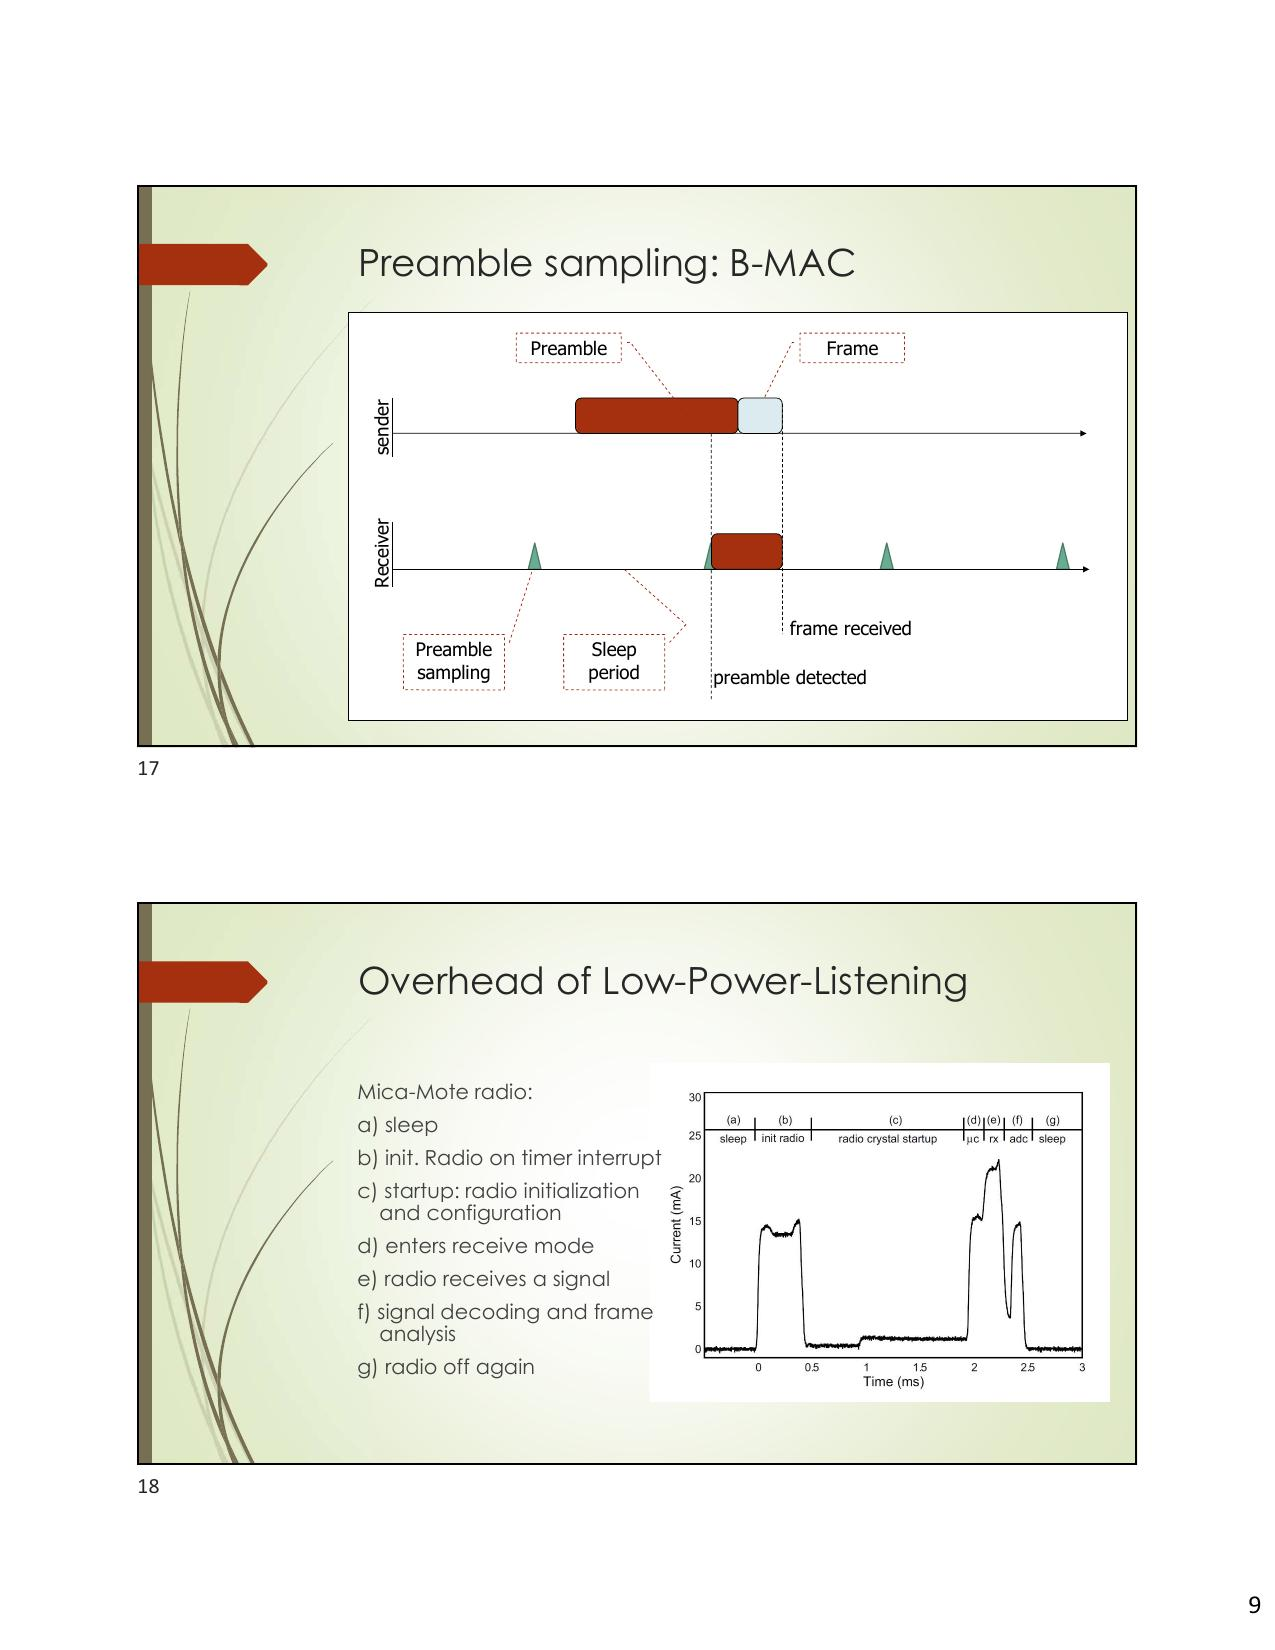
\includegraphics[keepaspectratio]{images/lezione-17-mac-protocols-img-05.jpg}}
\caption{Profilo di corrente (mA) nel tempo (ms) durante un ciclo di
Low-Power Listening: sleep → init → startup → receive mode → ricezione
segnale → decoding → sleep. Le fasi (a)-(g) evidenziano i picchi di
consumo durante l'attivazione.}
\end{figure}

\subsection{Bilanciamento energetico}\label{bilanciamento-energetico}

Il principio di B-MAC è spostare il costo energetico dalla ricezione
alla trasmissione:

\begin{itemize}
\tightlist
\item
  \textbf{Ricevitore}: risparmia molto perché esegue solo brevi
  campionamenti periodici (molto economici) invece di tenere la radio
  sempre accesa.
\item
  \textbf{Trasmittente}: spende di più perché deve trasmettere un
  preambolo lunghissimo (dell'ordine di 113 ms per il CC1000) prima di
  ogni frame dati.
\end{itemize}

\begin{callouttip}{Intuizione chiave}

Il preambolo deve essere più lungo del periodo di sleep! Se il
ricevitore dorme per \(T_{sleep}\), il preambolo deve durare almeno
\(T_{sleep}\) per garantire che il ricevitore lo intercetti durante il
suo campionamento.

\end{callouttip}

\subsection{Modello energetico}\label{modello-energetico}

Definiamo i parametri: - \(f_d\) = frequenza di trasmissione dei dati
(Hz) - \(f_c\) = frequenza di campionamento del preambolo (preamble
sampling rate) - \(p_t\) = potenza in trasmissione - \(p_r\) = potenza
in ricezione - \(p_i\) = potenza in idle (radio accesa ma non trasmette
né riceve)

Per il \textbf{trasmittente}, il duty cycle è:

\[DC_{data} = f_d \cdot (t_{preamble} + t_{frame})\]
\[DC_{check} = f_d \cdot t_{check}\]

L'energia consumata in \(t\) secondi è:

\[E_T(t) = t \left[ p_t \cdot DC_{data} + p_r \cdot DC_{check} + p_i \cdot (1 - DC_{data} - DC_{check}) \right]\]

Per il \textbf{ricevitore}:

\[DC_{data} = f_c \cdot (t_{listen} + t_{data})\]
\[DC_{check} = f_c \cdot t_{check}\]

\[E_R(t) = t \left[ p_r \cdot DC_{data} + p_r \cdot DC_{check} + p_i \cdot (1 - DC_{data} - DC_{check}) \right]\]

Da questi, la \textbf{lifetime} della batteria è:

\[lifetime_T = \frac{battery}{E_T(1)}, \quad lifetime_R = \frac{battery}{E_R(1)}\]

\subsection{Parametri reali (CC1000
radio)}\label{parametri-reali-cc1000-radio}

{\def\LTcaptype{none} % do not increment counter
\begin{longtable}[]{@{}ll@{}}
\toprule\noalign{}
Parametro & Valore \\
\midrule\noalign{}
\endhead
\bottomrule\noalign{}
\endlastfoot
\(p_t\) (trasmissione) & 60 mW \\
\(p_r\) (ricezione) & 45 mW \\
\(p_i\) (idle) & 0,09 mW \\
Lunghezza preambolo & 271 byte (113 ms) \\
Frame dati & 36 byte (15 ms) \\
Durata check & 0,35 ms \\
\end{longtable}
}

L'analisi numerica mostra che la lifetime sia del trasmittente sia del
ricevitore dipende fortemente dall'\textbf{intervallo di check} (il
periodo di sleep tra un campionamento e l'altro) e dal \textbf{traffico
nella cella}. Esiste un intervallo di check ottimale che massimizza la
lifetime per ciascun tasso di campionamento dei dati: campionamenti radi
dei dati permettono check interval più lunghi (e quindi meno
campionamenti del preambolo), massimizzando la durata della batteria.

\begin{calloutnote}{Nota sulla scalabilità}

Il modello mostra che anche considerando più trasmittenti contemporanei,
il trend della lifetime non cambia qualitativamente. La lifetime dipende
principalmente dall'intervallo di check e dalla quantità di traffico
nella cella radio.

\end{calloutnote}

\subsection{Punti di forza e limiti di
B-MAC}\label{punti-di-forza-e-limiti-di-b-mac}

\textbf{Punti di forza:} - Non è un protocollo di organizzazione di rete
(non impone strutture topologiche). - Semplicissimo da configurare: un
solo parametro, l'intervallo di check. - Trasparente ai livelli
superiori dello stack.

\textbf{Limiti:} - Preamboli lunghi hanno un costo energetico elevato
per il trasmittente. - All'aumentare dell'intervallo di check (per
risparmiare in ricezione), il preambolo deve allungarsi, aumentando il
costo in trasmissione. - In scenari con traffico elevato può risultare
meno efficiente della sincronizzazione.

\begin{center}\rule{0.5\linewidth}{0.5pt}\end{center}

\section{Preamble Sampling: X-MAC}\label{preamble-sampling-x-mac}

X-MAC è un'evoluzione diretta di B-MAC che risponde alla domanda:
\emph{si può ridurre il costo del lungo preambolo?} La risposta è sì,
inserendo nel preambolo l'\textbf{indirizzo del destinatario}.

Il meccanismo funziona così:

\begin{enumerate}
\def\labelenumi{\arabic{enumi}.}
\tightlist
\item
  Il mittente inizia a trasmettere preamboli brevi ripetuti, ciascuno
  contenente l'ID del ricevitore target.
\item
  I nodi che non sono il destinatario ignorano il preambolo.
\item
  Il destinatario, al primo campionamento, riconosce il proprio ID,
  \textbf{interrompe il preambolo} inviando un acknowledgement, e
  richiede il frame.
\item
  Il mittente smette di trasmettere il preambolo e invia direttamente il
  frame.
\end{enumerate}

\begin{callouttip}{Intuizione chiave}

In B-MAC il preambolo deve durare almeno \(T_{sleep}\) indipendentemente
da quando il ricevitore si sveglia. Con X-MAC, la durata effettiva del
preambolo è solo il tempo che intercorre tra l'inizio della trasmissione
e il momento in cui il ricevitore fa il campionamento: in media
\(T_{sleep}/2\).

\end{callouttip}

Simulazioni su reti a stella (un ricevitore, più trasmittenti) mostrano
che X-MAC riduce significativamente il duty cycle totale rispetto a
B-MAC, specialmente con intervalli di check più lunghi.

\begin{center}\rule{0.5\linewidth}{0.5pt}\end{center}

\begin{figure}
\centering
\pandocbounded{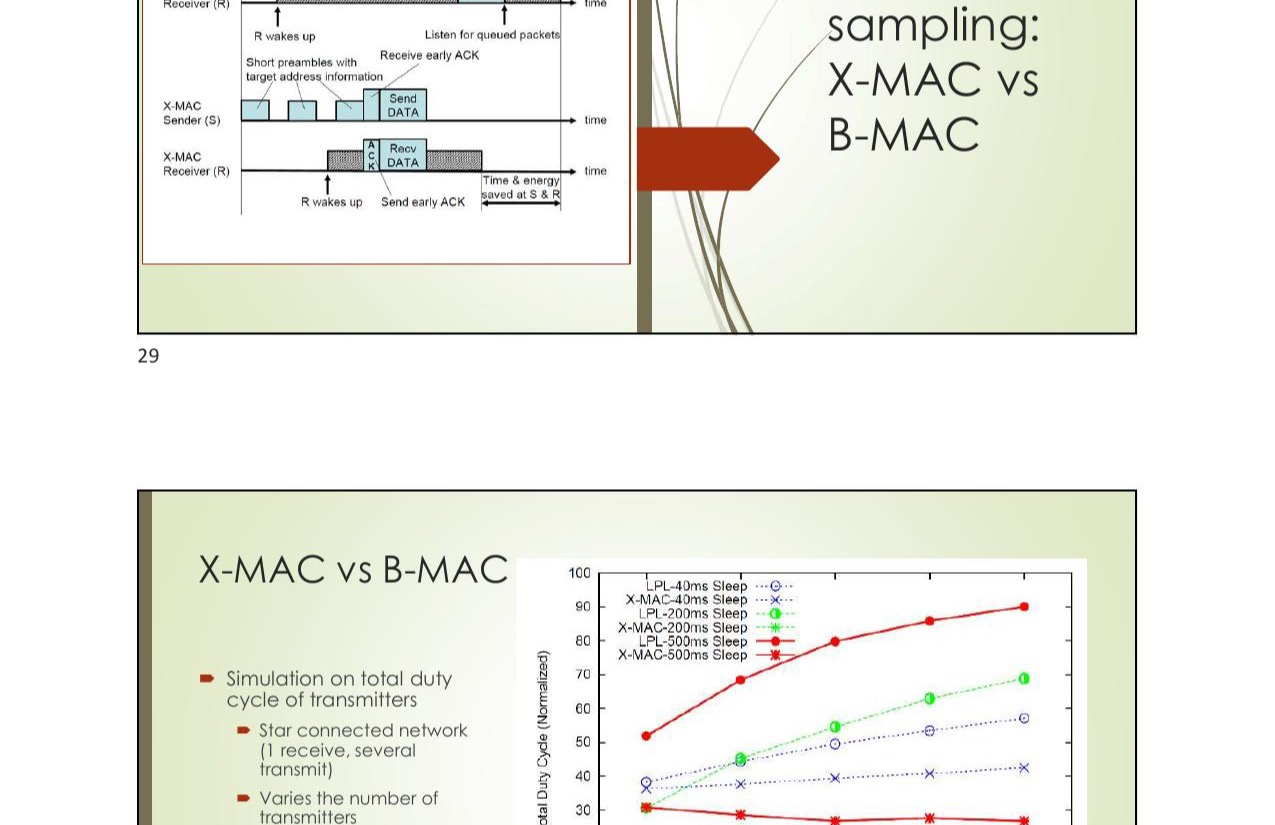
\includegraphics[keepaspectratio]{images/lezione-17-mac-protocols-img-06.jpg}}
\caption{In B-MAC il preambolo dura per tutta la finestra di sleep del
ricevitore. In X-MAC il preambolo è una sequenza di frame corti con l'ID
del destinatario: il ricevitore interrompe la trasmissione appena si
sveglia, riducendo tempo ed energia spesi.}
\end{figure}

\begin{figure}
\centering
\pandocbounded{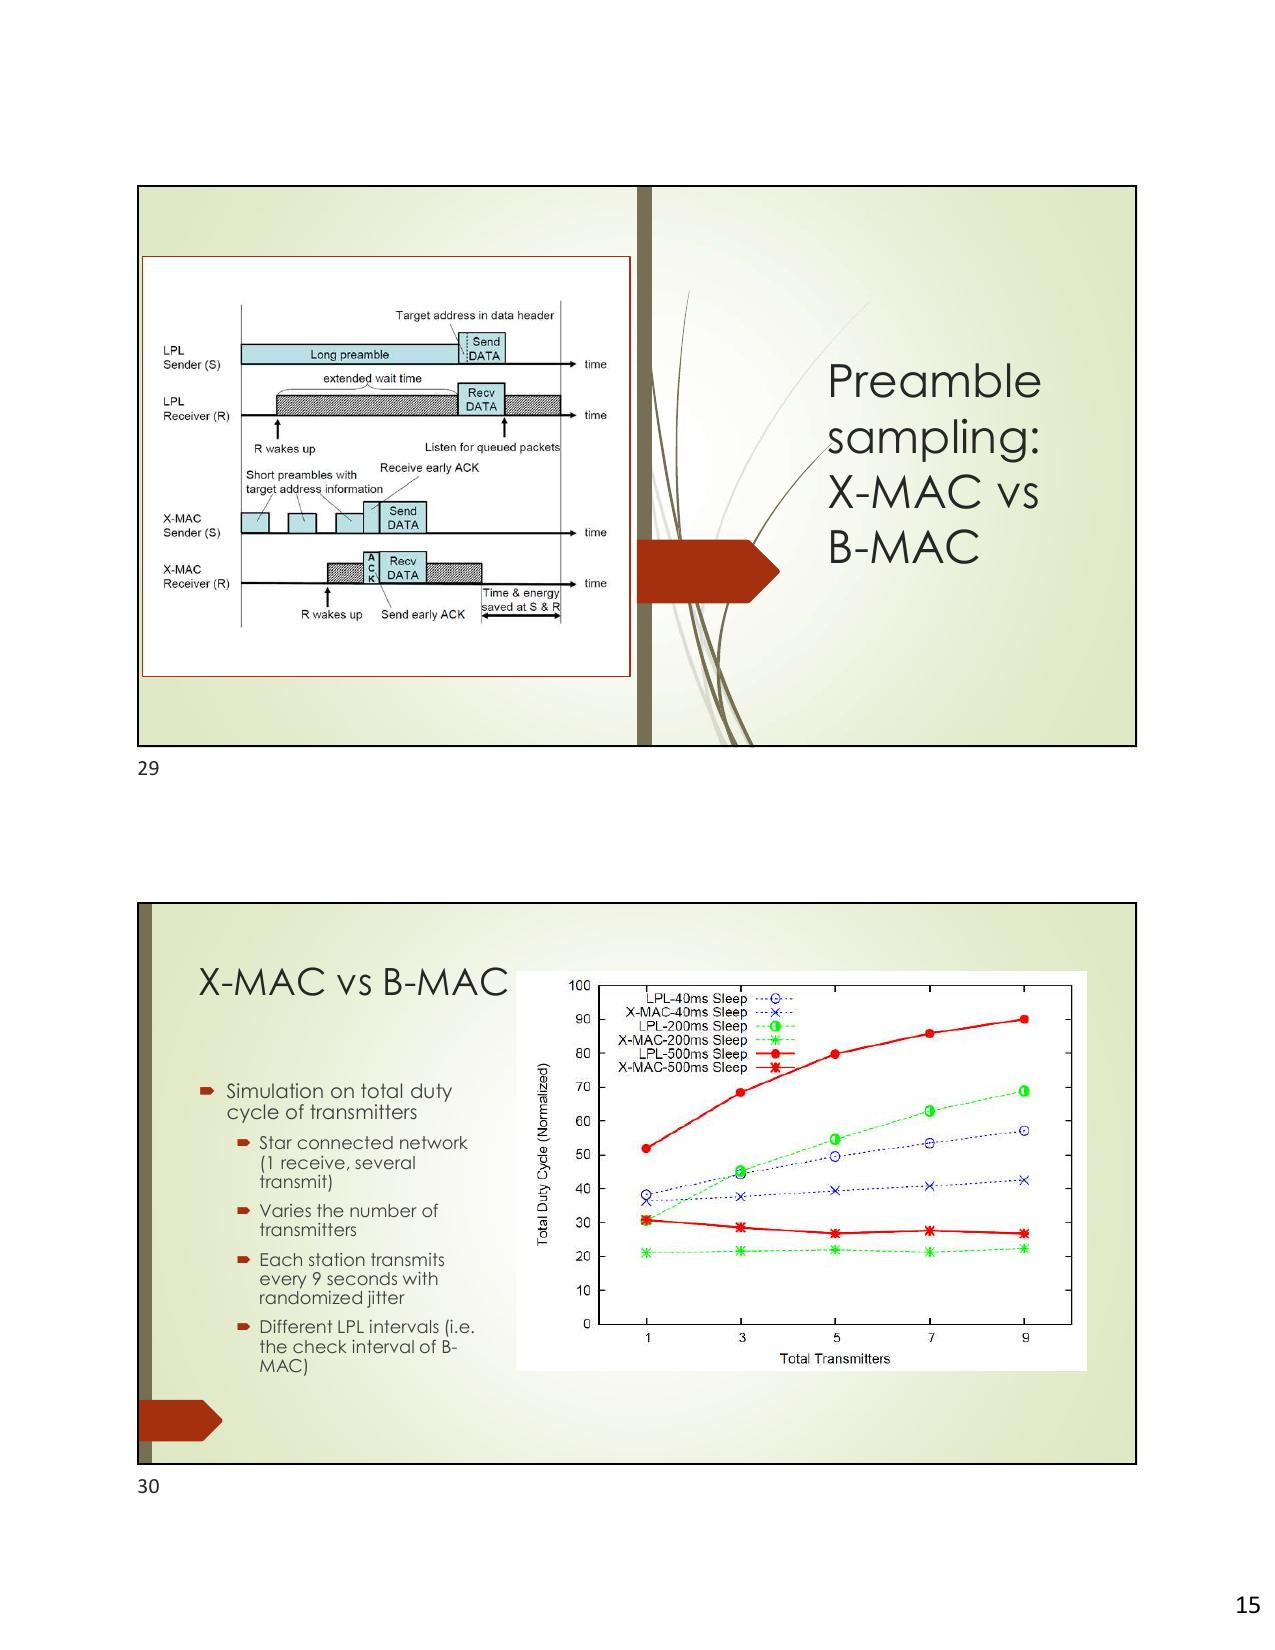
\includegraphics[keepaspectratio]{images/lezione-17-mac-protocols-img-07.jpg}}
\caption{Simulazione su rete a stella. X-MAC (curve in basso) mantiene
un duty cycle significativamente inferiore rispetto a B-MAC (curve in
alto) per tutti gli intervalli LPL e al crescere del numero di
trasmittenti.}
\end{figure}

\section{Preamble Sampling: BoX-MAC}\label{preamble-sampling-box-mac}

BoX-MAC (\emph{Backoff X-MAC}) è un ulteriore sviluppo di X-MAC. L'idea
chiave è che il preambolo stesso diventa una \textbf{sequenza ripetuta
del frame dati reale}.

Il funzionamento è il seguente:

\begin{enumerate}
\def\labelenumi{\arabic{enumi}.}
\tightlist
\item
  Il mittente trasmette ripetutamente l'intero frame (header + payload).
\item
  Il ricevitore, al campionamento, intercetta un'istanza del frame.
\item
  Se è il destinatario, aspetta il boundary del frame successivo, lo
  riceve completamente, invia un ACK per fermare il trasmittente.
\end{enumerate}

Questa strategia elimina la distinzione tra preambolo e frame: il
``preambolo'' è il frame stesso, e il ricevitore non deve aspettare la
fine del preambolo per ricevere i dati --- basta aspettare il prossimo
frame della sequenza. Funziona bene con \textbf{frame di piccole
dimensioni}, che è il caso tipico nelle reti di sensori.

In scenari multi-hop, BoX-MAC mostra comportamenti interessanti: i nodi
intermedi possono eventualmente ``sentire'' i frame ripetuti e
anticipare il routing, riducendo ulteriormente la latenza end-to-end.

\begin{center}\rule{0.5\linewidth}{0.5pt}\end{center}

\begin{figure}
\centering
\pandocbounded{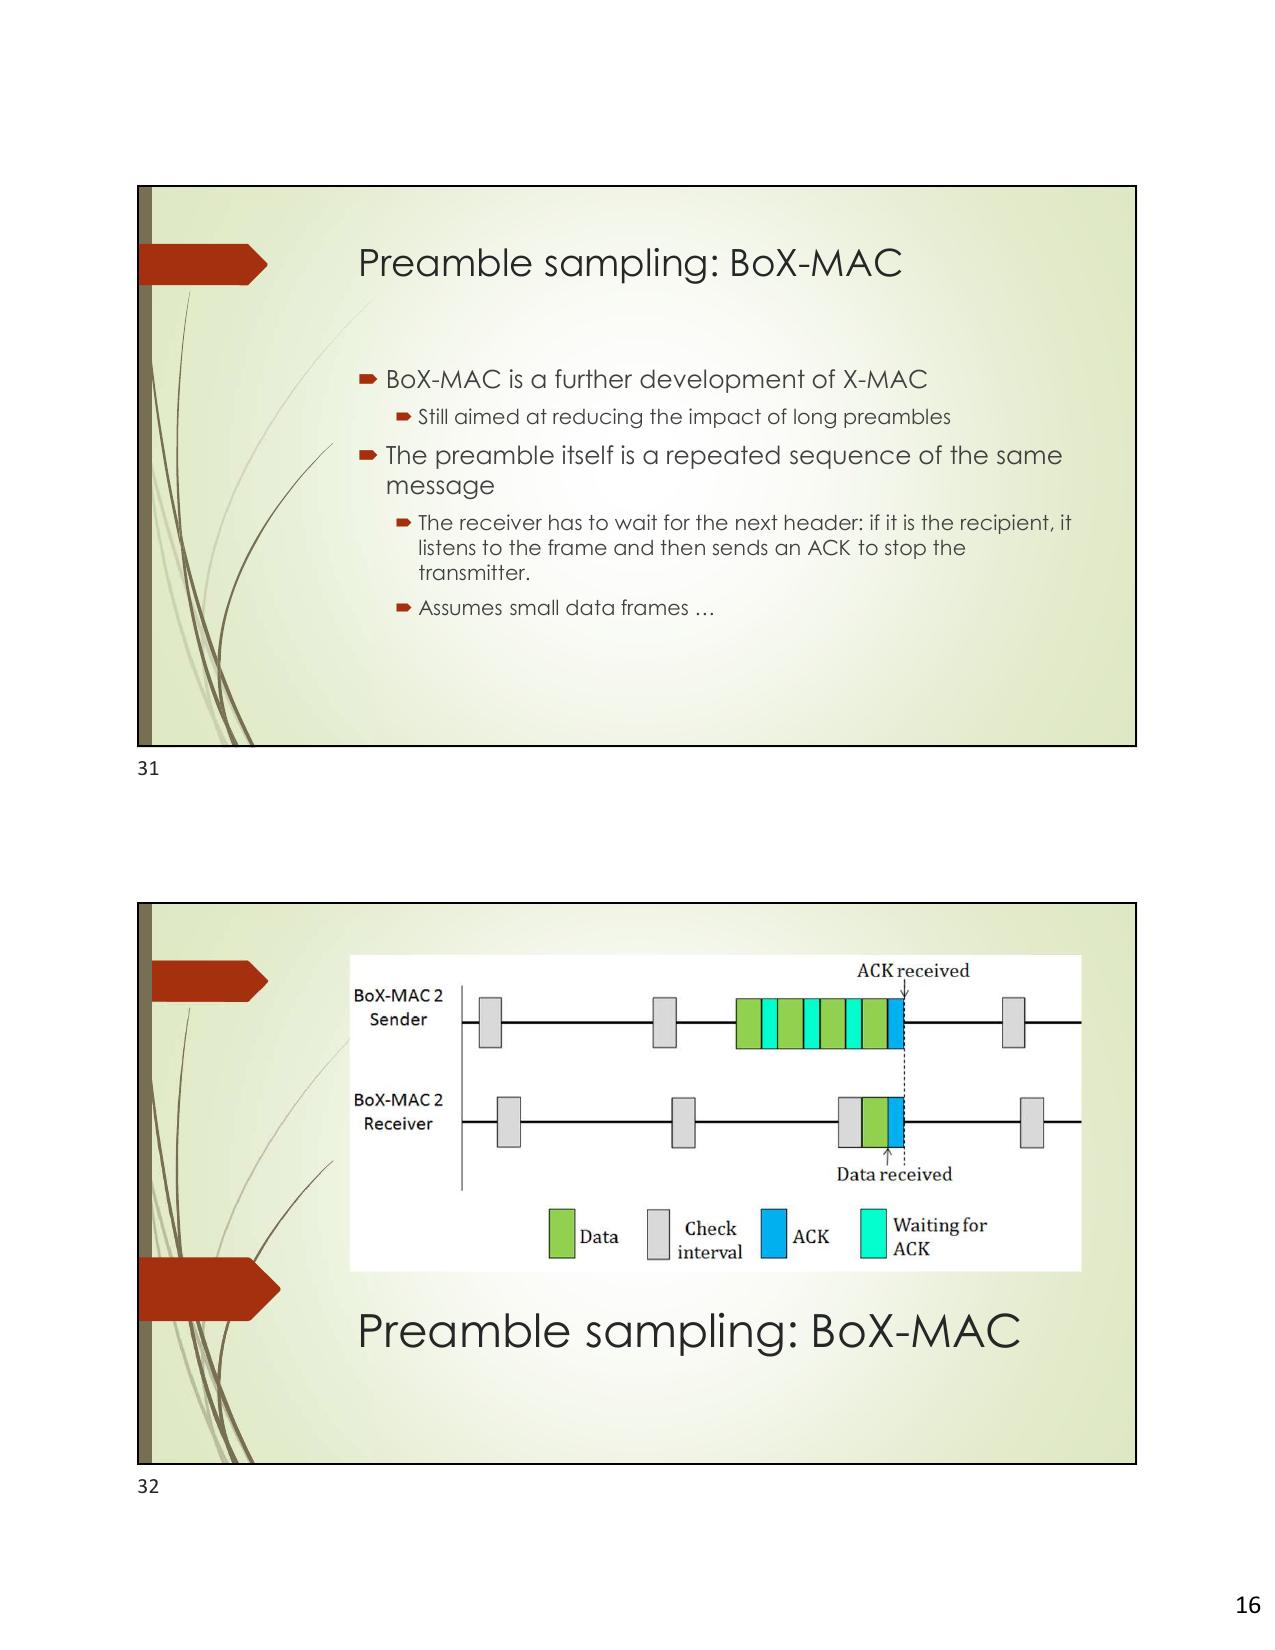
\includegraphics[keepaspectratio]{images/lezione-17-mac-protocols-img-08.jpg}}
\caption{Il mittente ripete il frame più volte. Il ricevitore, al
campionamento, aspetta il boundary del frame successivo, lo riceve, e
invia un ACK per fermare la trasmissione. La legenda mostra Data TX,
Data RX, ACK, y (sync) e channel sampling.}
\end{figure}

\begin{figure}
\centering
\pandocbounded{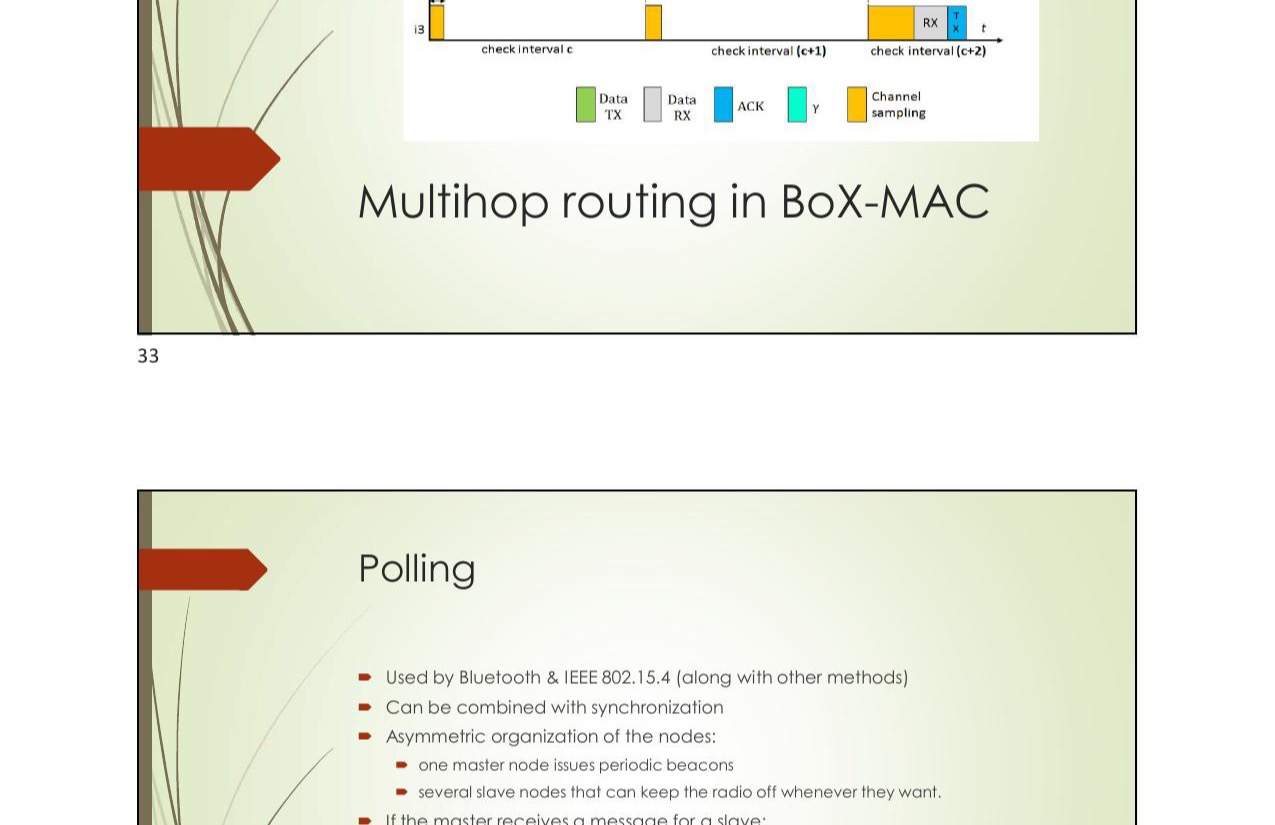
\includegraphics[keepaspectratio]{images/lezione-17-mac-protocols-img-09.jpg}}
\caption{Tre nodi i1, i2, i3 in cascata. Il nodo i1 trasmette
ripetutamente; i2 riceve nel proprio check interval e ritrasmette a i3;
i3 riceve nel check interval successivo. Il DUTY\_ON\_TIME mostra il
tempo totale di attività della radio per ciascun nodo.}
\end{figure}

\section{Polling}\label{polling}

Il polling è il terzo approccio all'efficienza energetica, usato da
\textbf{Bluetooth} e \textbf{IEEE 802.15.4} (in combinazione con la
sincronizzazione). Richiede un'\textbf{organizzazione asimmetrica} della
rete:

\begin{itemize}
\tightlist
\item
  Un nodo \textbf{master} trasmette periodicamente dei \textbf{beacon}.
\item
  I nodi \textbf{slave} possono tenere la radio spenta quando vogliono,
  senza coordinazione.
\end{itemize}

Il meccanismo per la consegna dei messaggi verso uno slave è il
seguente:

\begin{enumerate}
\def\labelenumi{\arabic{enumi}.}
\tightlist
\item
  Se il master riceve un messaggio destinato a uno slave, lo memorizza.
\item
  Il master annuncia nel beacon che c'è un messaggio in attesa per
  quello slave.
\item
  Quando lo slave si sveglia, aspetta il beacon, riconosce il pending
  message, e invia una richiesta esplicita al master.
\item
  Il master consegna il frame.
\end{enumerate}

\begin{calloutnote}{Nota}

Il polling è intrinsecamente compatibile con la sincronizzazione: i
beacon del master possono servire anche da segnale di sincronizzazione
per i nodi slave. IEEE 802.15.4 usa esattamente questa combinazione
nella sua modalità con beacon.

\end{calloutnote}

\begin{center}\rule{0.5\linewidth}{0.5pt}\end{center}

\section{Domande d'esame}\label{domande-desame}

\newpage

\chapter{Lo Standard IEEE 802.15.4}\label{lo-standard-ieee-802.15.4}

Lo standard IEEE 802.15.4 definisce le specifiche del \textbf{physical
layer} e del \textbf{MAC layer} per le \textbf{Low-Rate Wireless
Personal Area Network} (\emph{LR-WPAN}, reti personali senza fili a
bassa velocità). L'obiettivo è fornire un protocollo radio
standardizzato per dispositivi a risorse limitate --- sensori,
attuatori, nodi IoT --- che richiedono bassi consumi energetici
piuttosto che elevate velocità di trasmissione.

\begin{calloutdefinition}{IEEE 802.15.4}

Specifica del physical layer e del MAC layer per reti LR-WPAN
(\emph{Low-Rate Wireless Personal Area Network}). Supporta comunicazioni
a corto raggio, bassa velocità di trasmissione e coesistenza con IEEE
802.11 (Wi-Fi) e IEEE 802.15.1 (Bluetooth).

\end{calloutdefinition}

Una caratteristica progettuale importante è la coesistenza con altri
standard wireless: il physical layer è disegnato per poter operare nello
stesso ambiente fisico di IEEE 802.11 e IEEE 802.15.1 senza causare
interferenze reciproche devastanti.

\section{Bande di Frequenza}\label{bande-di-frequenza}

Lo standard opera su tre bande di frequenza libere da licenza
(\emph{licence-free}):

{\def\LTcaptype{none} % do not increment counter
\begin{longtable}[]{@{}llll@{}}
\toprule\noalign{}
Banda & Regione & Data rate & Canali \\
\midrule\noalign{}
\endhead
\bottomrule\noalign{}
\endlastfoot
868--868.6 MHz & Europa & 20 kbps & 1 (canale 0) \\
902--928 MHz & Nord America & 40 kbps & 10 (canali 1--10) \\
2400--2483.5 MHz & Mondiale & 250 kbps & 16 (canali 11--26) \\
\end{longtable}
}

La banda a 2.4 GHz è quella più diffusa perché disponibile a livello
globale e garantisce la velocità di trasmissione più alta. La banda a
868 MHz --- tipicamente utilizzata in Europa --- è quella con il data
rate più basso ma offre maggiore robustezza in ambienti con SNR basso.

\begin{callouttip}{Esempio: banda 868 MHz}

\begin{itemize}
\tightlist
\item
  Frequenza centrale: 868.3 MHz
\item
  Data rate: 20 kbps
\item
  Modulazione: simboli binari
\item
  Un solo canale disponibile
\item
  Dimensione massima del pacchetto: 127 byte
\end{itemize}

\end{callouttip}

\begin{center}\rule{0.5\linewidth}{0.5pt}\end{center}

\section{Physical Layer}\label{physical-layer}

Il \textbf{physical layer} di IEEE 802.15.4 eroga due categorie di
servizi verso lo strato superiore: servizi dati e servizi di gestione.

\subsection{Servizi del Physical
Layer}\label{servizi-del-physical-layer}

Il \textbf{Data Service} è responsabile della trasmissione e ricezione
delle \textbf{PPDU} (\emph{PHY Protocol Data Unit}) attraverso il mezzo
fisico. Quando una trasmissione fallisce, il physical layer riporta
all'upper layer il motivo del fallimento: il ricetrasmettitore potrebbe
essere guasto, in modalità ricezione, oppure già impegnato in un'altra
operazione.

Il \textbf{Management Service} comprende un insieme più ampio di
funzionalità:

\begin{itemize}
\tightlist
\item
  Attivazione e disattivazione del ricetrasmettitore radio, per
  implementare politiche di risparmio energetico.
\item
  \textbf{Energy Detection} (ED): misura del livello di energia sul
  canale.
\item
  \textbf{Link Quality Indicator} (LQI): stima della qualità dei
  pacchetti ricevuti.
\item
  \textbf{Channel Selection}: selezione del canale operativo.
\item
  \textbf{Clear Channel Assessment} (CCA): verifica se il canale è
  libero prima di trasmettere.
\item
  Configurazione della \textbf{PHY-PIB} (\emph{PHY PAN Information
  Base}), la struttura dati che mantiene i parametri di configurazione
  del physical layer.
\end{itemize}

\subsection{Prestazioni del Physical
Layer}\label{prestazioni-del-physical-layer}

\begin{figure}
\centering
\pandocbounded{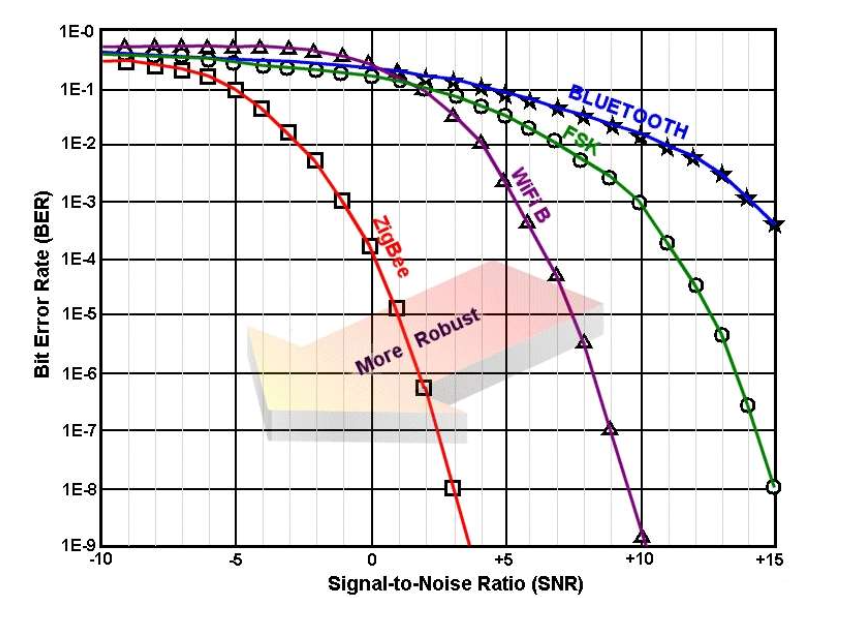
\includegraphics[keepaspectratio]{images/Pasted-image-20260408111308.png}}
\caption{Confronto di Bit Error Rate (BER) in funzione del SNR tra IEEE
802.15.4 (zona ``More Robust''), Bluetooth e altri standard. Lo standard
mostra eccellenti prestazioni in ambienti a basso SNR.}
\end{figure}

Il grafico mostra che IEEE 802.15.4 mantiene un BER molto basso anche in
condizioni di SNR negativo, dove altri standard (come Bluetooth) già
soffrono di errori frequenti. Questa robustezza è fondamentale per i
tipici ambienti IoT industriali o domestici, dove il canale radio è
spesso disturbato.

\subsection{Energy Detection}\label{energy-detection}

L'\textbf{Energy Detection} (ED) è il meccanismo utilizzato per trovare
un canale libero e per il \emph{carrier sense}. Il physical layer misura
la potenza del segnale sul canale su un intervallo di \textbf{8 simboli}
e confronta il risultato con una soglia fissata a \textbf{10 dB sopra il
livello di sensibilità} del ricevitore. Il risultato della rilevazione è
restituito come un valore a un byte.

\begin{calloutdefinition}{Energy Detection (ED)}

Stima del livello di energia media sul canale su una finestra di 8
simboli. Se l'energia supera la soglia (10 dB sopra la sensibilità), il
canale è considerato occupato.

\end{calloutdefinition}

\subsection{Link Quality Indicator}\label{link-quality-indicator}

Il \textbf{Link Quality Indicator} (LQI) misura la qualità dei pacchetti
dati ricevuti da un nodo. Viene valutato ogni volta che si riceve un
pacchetto e il suo valore viene propagato verso i layer di rete e
applicazione, dove può essere impiegato nel routing multi-hop --- ad
esempio in ZigBee --- per scegliere il percorso di qualità migliore.

\begin{calloutdefinition}{Link Quality Indicator (LQI)}

Indicatore di qualità del collegamento radio stimato su ogni pacchetto
ricevuto. Basato sull'ED, sul rapporto segnale/rumore o su una
combinazione di entrambi. Deve avere almeno 8 livelli distinti.

\end{calloutdefinition}

\subsection{Clear Channel Assessment}\label{clear-channel-assessment}

Il \textbf{Clear Channel Assessment} (CCA) determina se il canale è
occupato prima di trasmettere. Esistono tre modalità operative:

\begin{itemize}
\tightlist
\item
  \textbf{Modalità 1}: usa l'Energy Detection --- se l'energia supera la
  soglia, il canale è occupato.
\item
  \textbf{Modalità 2}: usa il \emph{Carrier Sense} --- il canale è
  occupato se il segnale rilevato ha le stesse caratteristiche del
  trasmettitore.
\item
  \textbf{Modalità 3}: combinazione delle modalità 1 e 2 in AND o OR.
\end{itemize}

\subsection{Struttura della PPDU}\label{struttura-della-ppdu}

Il frame del physical layer --- la \textbf{PPDU} (\emph{PHY Protocol
Data Unit}) --- è strutturato in tre sezioni principali:

\begin{figure}
\centering
\pandocbounded{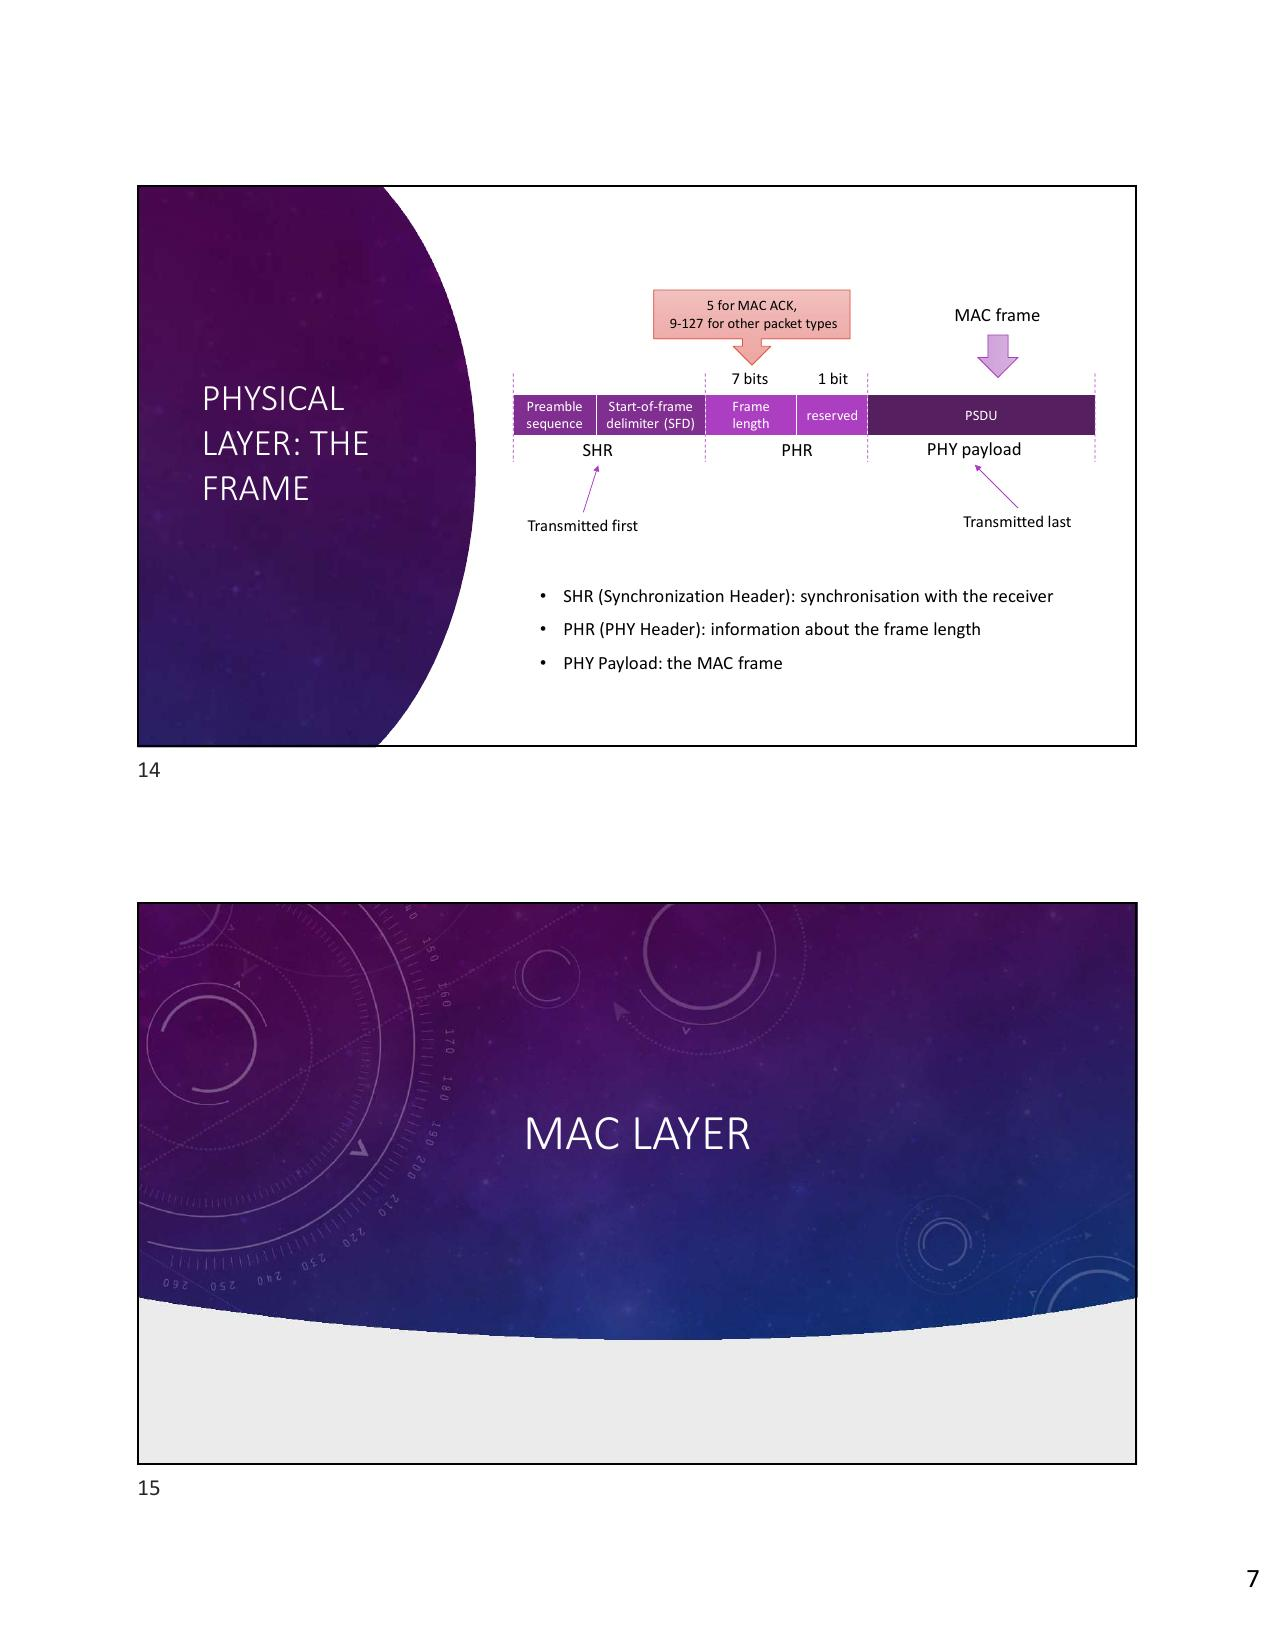
\includegraphics[keepaspectratio]{images/lezione-18-the-ieee-802-15-4-standard-img-01.jpg}}
\caption{Struttura della PPDU: SHR (Synchronization Header), PHR (PHY
Header) e PHY Payload (PSDU). Il frame viene trasmesso da sinistra
(preamble) a destra (payload MAC).}
\end{figure}

\begin{itemize}
\tightlist
\item
  \textbf{SHR} (\emph{Synchronization Header}): contiene la sequenza di
  preambolo e il delimitatore di inizio frame (SFD, \emph{Start-of-Frame
  Delimiter}). Permette al ricevitore di sincronizzarsi con il
  trasmettitore.
\item
  \textbf{PHR} (\emph{PHY Header}): contiene la lunghezza del frame su 7
  bit più 1 bit riservato. Il campo \emph{Frame length} può valere 5
  (per i MAC ACK) oppure da 9 a 127 per gli altri tipi di pacchetto.
\item
  \textbf{PHY Payload} (PSDU): il MAC frame incapsulato.
\end{itemize}

\begin{center}\rule{0.5\linewidth}{0.5pt}\end{center}

\section{MAC Layer}\label{mac-layer}

Il \textbf{MAC layer} di IEEE 802.15.4 si sovrappone al physical layer e
fornisce i meccanismi per l'accesso al mezzo condiviso, la
sincronizzazione, la formazione della rete e la sicurezza di base.

\subsection{Servizi del MAC Layer}\label{servizi-del-mac-layer}

\textbf{Data services}: trasmissione e ricezione di \textbf{MPDU}
(\emph{MAC Protocol Data Unit}) attraverso il physical layer.

\textbf{Management services}: sincronizzazione delle comunicazioni,
accesso al canale, gestione dei \textbf{Guaranteed Time Slot} (GTS),
associazione e disassociazione dei dispositivi alla rete.

\textbf{Security services}: cifratura dei dati, controllo degli accessi,
integrità dei frame, garanzie di freschezza sequenziale.

\subsection{Tipi di Dispositivi}\label{tipi-di-dispositivi}

\begin{calloutdefinition}{Reduced Function Device (RFD)}

Dispositivo con capacità ridotte di elaborazione, memoria e
comunicazione. Tipicamente sensori o attuatori semplici (interruttori,
lampade). Implementa solo un sottoinsieme del MAC layer: può associarsi
a una rete esistente, ma dipende da un FFD per comunicare. Ogni RFD può
essere associato a un solo FFD alla volta.

\end{calloutdefinition}

\begin{calloutdefinition}{Full Function Device (FFD)}

Implementa il MAC layer completo. Può fungere da coordinatore di PAN
(\emph{PAN coordinator}) o da coordinatore generico di un gruppo di RFD.
Il PAN coordinator seleziona l'identificatore di PAN e gestisce le
associazioni e disassociazioni dei dispositivi.

\end{calloutdefinition}

\subsection{Topologie di Rete}\label{topologie-di-rete}

Il MAC layer supporta due topologie fondamentali.

\textbf{Topologia a stella (Star)}: un unico FFD funge da PAN
coordinator; tutti gli altri nodi --- compresi eventuali FFD usati come
router --- comunicano esclusivamente con lui e si comportano come RFD.
Il PAN coordinator sincronizza tutte le comunicazioni nella rete. PAN
diverse hanno identificatori distinti e sono indipendenti.

\begin{figure}
\centering
\pandocbounded{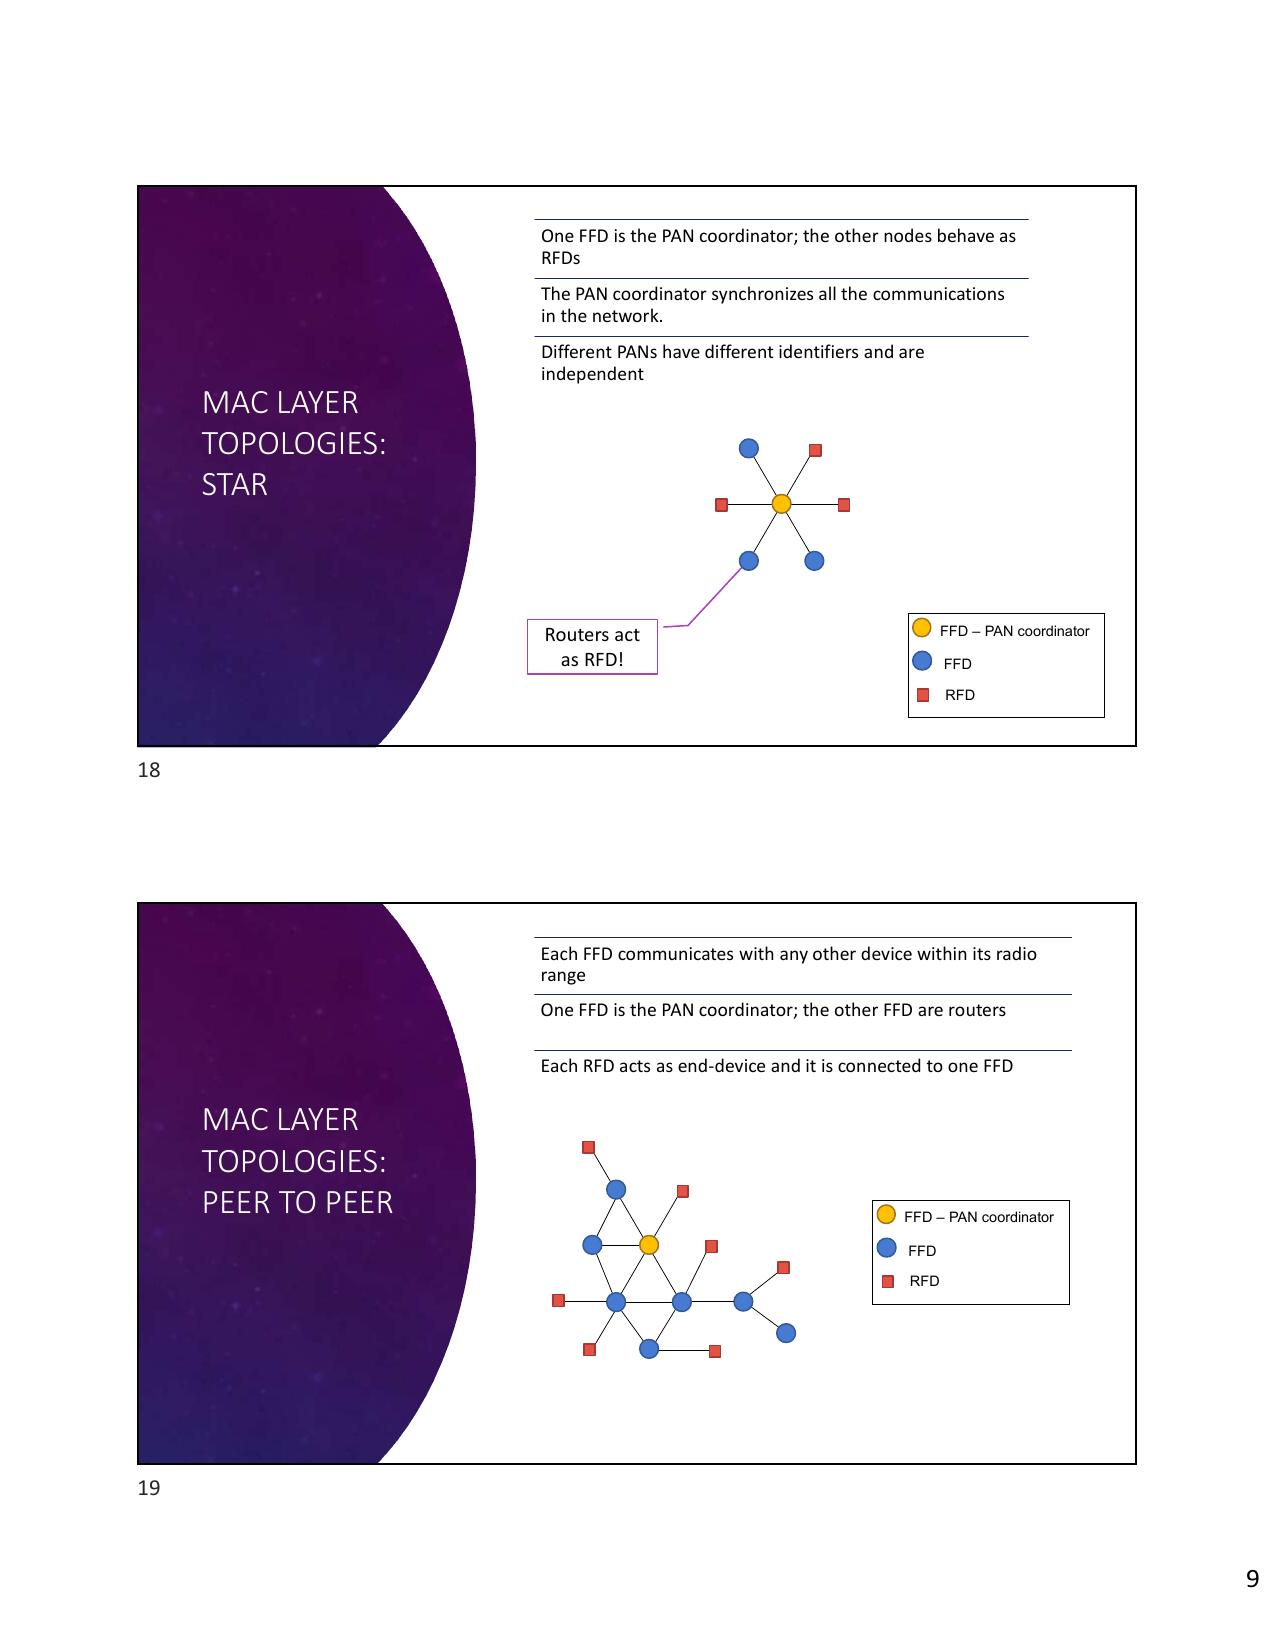
\includegraphics[keepaspectratio]{images/lezione-18-the-ieee-802-15-4-standard-img-02.jpg}}
\caption{Topologia Star: il PAN coordinator (arancione) al centro; FFD
blu e RFD rossi collegati direttamente. Anche i router agiscono come RFD
in questa topologia.}
\end{figure}

\textbf{Topologia peer-to-peer}: ogni FFD può comunicare con qualunque
altro dispositivo nel suo raggio radio. Un FFD è il PAN coordinator, gli
altri FFD sono router; ogni RFD è un end-device connesso a un FFD.
Questa topologia permette la formazione di reti mesh e alberi.

\begin{figure}
\centering
\pandocbounded{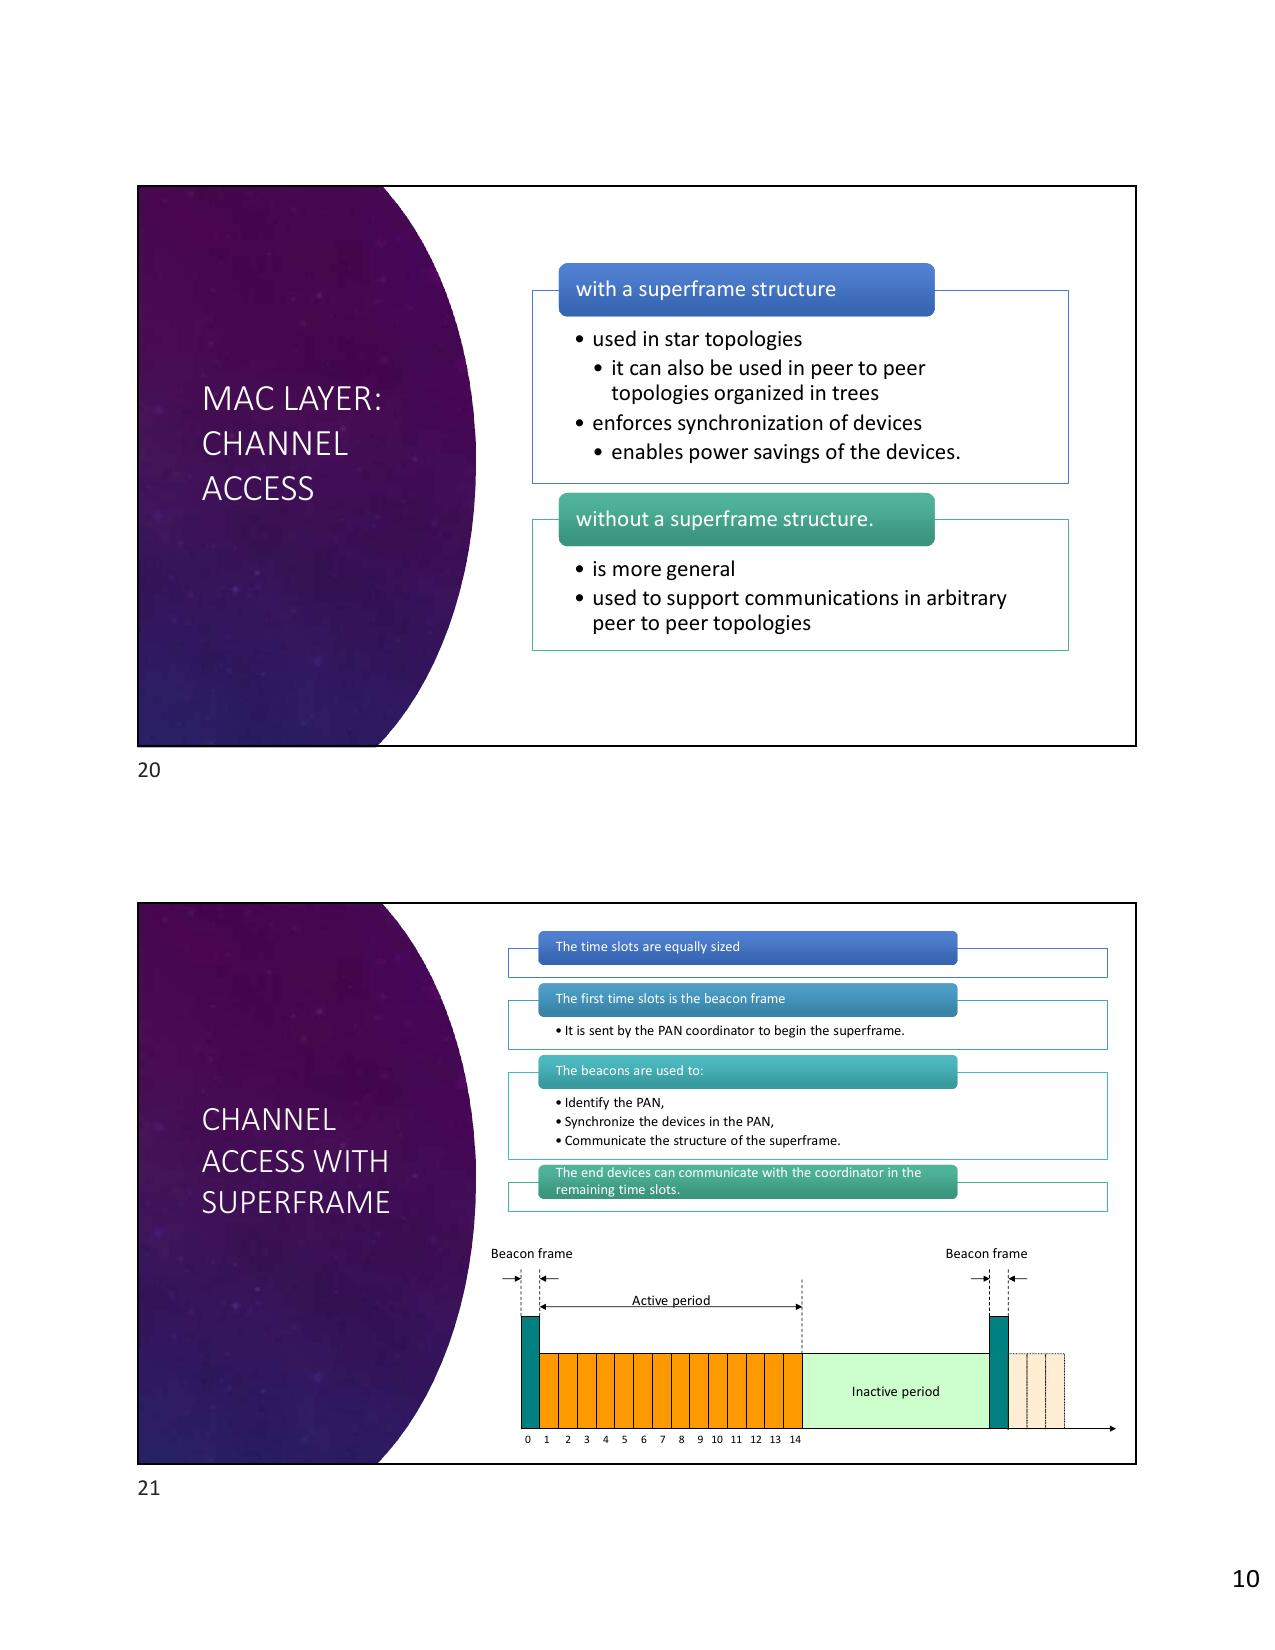
\includegraphics[keepaspectratio]{images/lezione-18-the-ieee-802-15-4-standard-img-03.jpg}}
\caption{Topologia Peer-to-Peer: gli FFD (blu) si interconnettono tra
loro; gli RFD (rosso) sono end-device connessi ciascuno a un FFD. Il PAN
coordinator è in arancione.}
\end{figure}

\subsection{Accesso al Canale con
Superframe}\label{accesso-al-canale-con-superframe}

La modalità \emph{beacon-enabled} struttura il tempo in
\textbf{superframe}, delimitati dall'invio periodico di un frame beacon
da parte del PAN coordinator. Il superframe divide il tempo in due
porzioni: una \textbf{active period} e una \textbf{inactive period}.
Durante il periodo inattivo il PAN coordinator e i dispositivi connessi
possono entrare in modalità a basso consumo (sleep).

La \textbf{active period} comprende fino a \textbf{16 time slot} di
uguale dimensione, suddivisi in:

\begin{itemize}
\tightlist
\item
  \textbf{CAP} (\emph{Contention Access Period}): fino a 15 slot. I
  dispositivi competono per il canale usando il protocollo
  \textbf{CSMA-CA a slot} (\emph{slotted CSMA-CA}). Un dispositivo
  attende un numero casuale di slot; se il canale è occupato riprova
  dopo un altro backoff casuale; se è libero trasmette e mantiene il
  canale fino alla fine del frame.
\item
  \textbf{CFP} (\emph{Contention Free Period}): opzionale, occupa gli
  ultimi slot del periodo attivo. Diviso in \textbf{GTS}
  (\emph{Guaranteed Time Slot}), ciascuno assegnato dal PAN coordinator
  a una specifica applicazione. Il GTS è accessibile senza CSMA-CA,
  garantendo latenza deterministica. Ogni CFP può contenere al massimo 7
  GTS, ciascuno composto da uno o più slot.
\end{itemize}

\begin{figure}
\centering
\pandocbounded{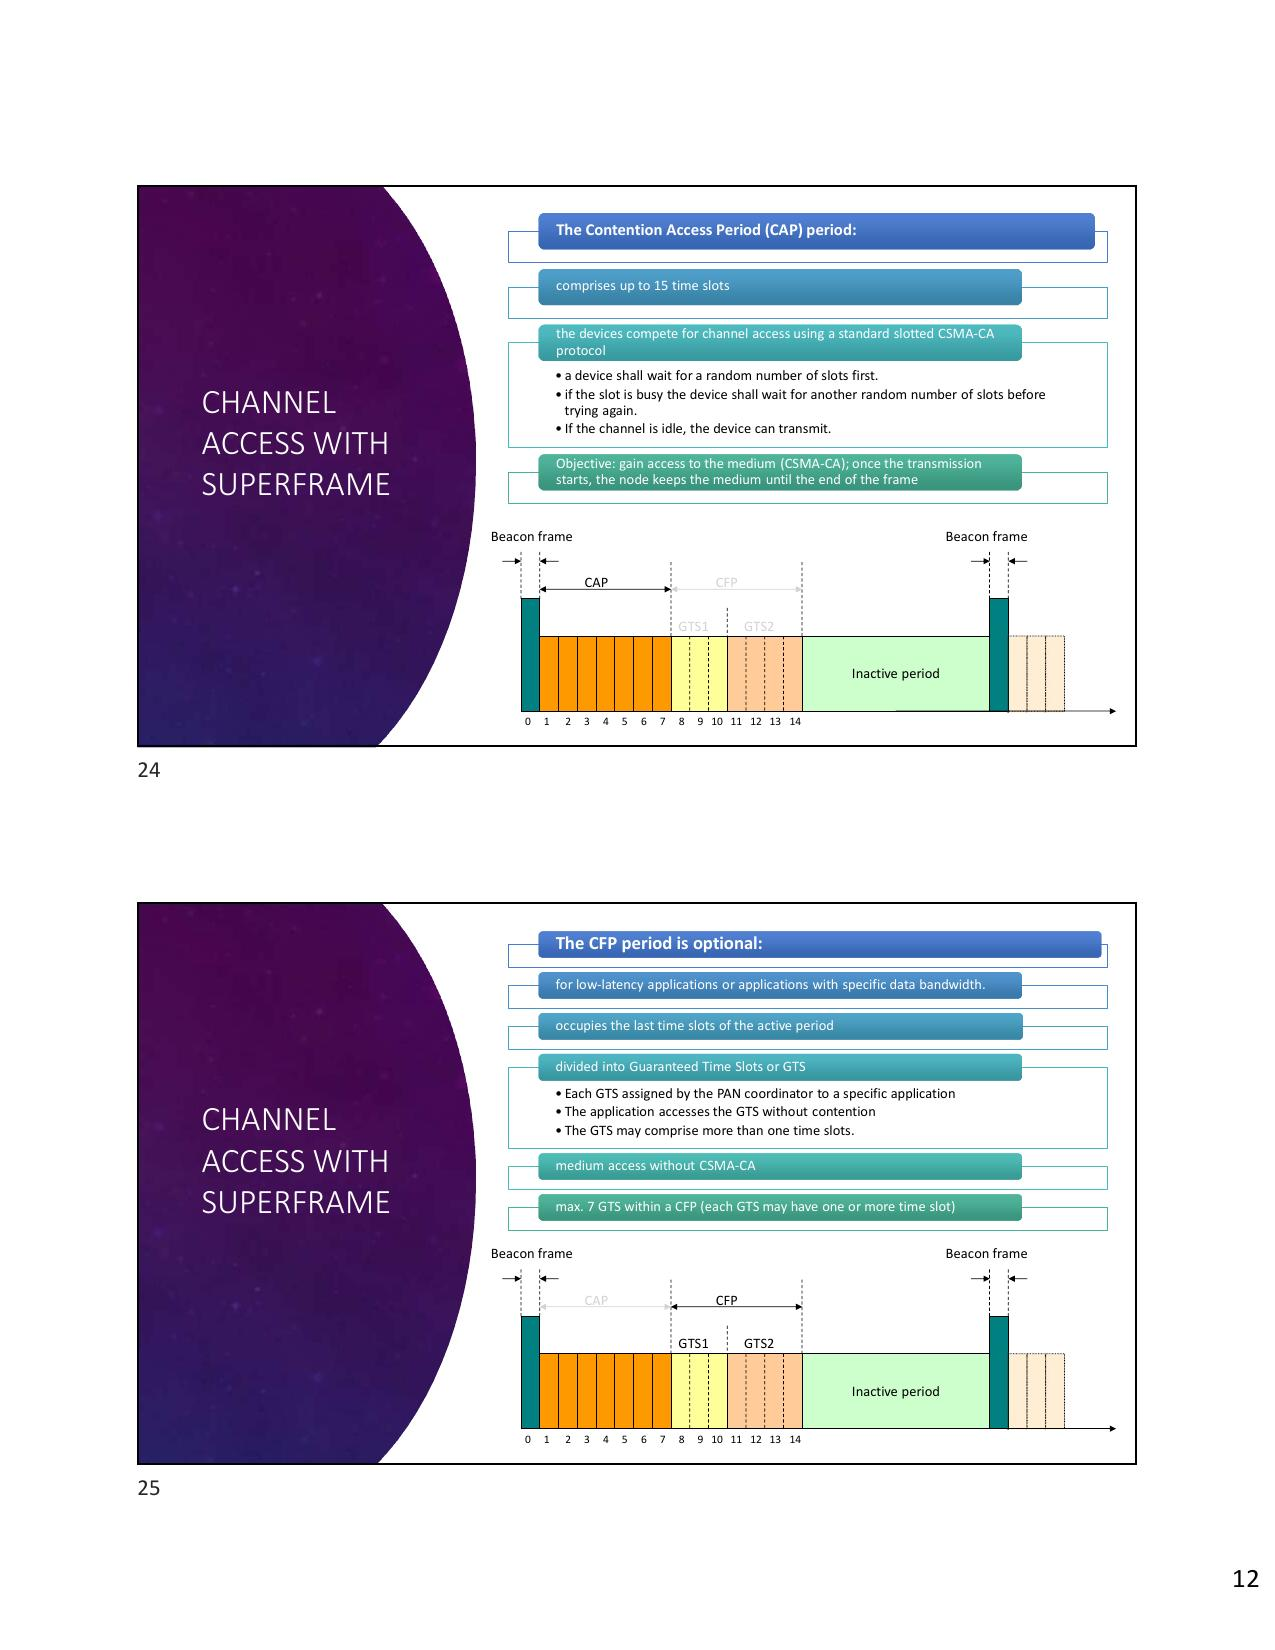
\includegraphics[keepaspectratio]{images/lezione-18-the-ieee-802-15-4-standard-img-04.jpg}}
\caption{Struttura del superframe: il beacon apre il periodo attivo,
diviso in CAP (accesso CSMA-CA, arancione) e CFP opzionale con GTS
(verde). Segue il periodo inattivo.}
\end{figure}

\begin{calloutwarning}{Il CAP non può essere eliminato}

Anche quando è presente il CFP, il CAP è necessario per il mantenimento
della rete: gestione di associazioni/disassociazioni, richieste di GTS,
ecc. Tutte le transazioni basate su contesa devono completarsi prima
dell'inizio del CFP. Un dispositivo che trasmette in un GTS deve
completare la trasmissione entro il suo GTS assegnato.

\end{calloutwarning}

\begin{callouttip}{Intuizione: CAP vs CFP}

Il CAP è come un incrocio senza precedenza fissa (tutti attendono il
proprio turno casuale). Il CFP è come una corsia riservata (accede solo
chi ha la prenotazione). Le applicazioni real-time o ad alta priorità
richiedono GTS nel CFP; le comunicazioni ordinarie usano il CAP.

\end{callouttip}

\subsection{Accesso al Canale senza
Superframe}\label{accesso-al-canale-senza-superframe}

Nella modalità \emph{non beacon-enabled}, non esiste struttura a
superframe. L'accesso al canale usa \textbf{CSMA-CA non a slot}
(\emph{unslotted CSMA-CA}). I coordinatori devono essere sempre attivi
per ricevere dati dagli end-device.

Il trasferimento in direzione coordinatore → end-device è basato su
polling: l'end-device si sveglia periodicamente e interroga il
coordinatore per verificare se ci sono messaggi in attesa. Il
coordinatore risponde con il messaggio pendente o segnala che non ve ne
sono.

\begin{center}\rule{0.5\linewidth}{0.5pt}\end{center}

\section{Modalità di Trasferimento
Dati}\label{modalituxe0-di-trasferimento-dati}

IEEE 802.15.4 definisce tre direzioni di trasferimento dati:

\begin{enumerate}
\def\labelenumi{\arabic{enumi}.}
\tightlist
\item
  \textbf{End-device → coordinatore (o router)}
\item
  \textbf{Coordinatore (o router) → end-device}
\item
  \textbf{Peer-to-peer}
\end{enumerate}

La topologia a stella usa solo le modalità 1 e 2. La peer-to-peer le
supporta tutte e tre.

\subsection{Trasferimento in Reti
Beacon-Enabled}\label{trasferimento-in-reti-beacon-enabled}

\textbf{Da end-device a coordinatore}: il dispositivo attende il beacon
per sincronizzarsi. Se possiede un GTS lo usa senza contesa; altrimenti
trasmette nel CAP usando CSMA-CA a slot. Il coordinatore può inviare un
ACK opzionale.

\textbf{Da coordinatore a end-device}: il coordinatore memorizza il
messaggio e segnala nel beacon che c'è un messaggio pendente.
L'end-device, che dorme la maggior parte del tempo, ascolta
occasionalmente il beacon. Quando rileva un messaggio pendente invia un
\emph{Data request} nel CAP (con ACK immediato dal coordinatore). Il
coordinatore trasmette il messaggio in uno slot successivo del CAP;
l'end-device invia un ACK obbligatorio. Infine il coordinatore rimuove
il messaggio dalla lista.

\textbf{Peer-to-peer}: tra coordinatore/router e end-device si applicano
gli schemi precedenti. Due end-device non possono comunicare
direttamente. La comunicazione tra due coordinatori o tra coordinatore e
router richiede che il mittente si sincronizzi con il beacon del
destinatario --- ma le modalità per farlo sono fuori dallo scope dello
standard.

\subsection{Trasferimento in Reti Non
Beacon-Enabled}\label{trasferimento-in-reti-non-beacon-enabled}

\textbf{Da end-device a coordinatore}: il dispositivo trasmette
direttamente con CSMA-CA non a slot; il coordinatore deve essere sempre
attivo. L'ACK è opzionale.

\textbf{Da coordinatore a end-device}: il coordinatore memorizza il
messaggio; l'end-device interroga periodicamente il coordinatore con una
\emph{Data request} (CSMA-CA non a slot), riceve ACK, poi il messaggio,
poi invia l'ACK finale. Se non ci sono messaggi pendenti il coordinatore
risponde con un messaggio vuoto.

\textbf{Peer-to-peer}: ogni dispositivo può comunicare con ogni altro
nel suo raggio radio. I dispositivi devono restare sempre attivi oppure
sincronizzarsi tra loro --- ma la sincronizzazione è delegata ai layer
superiori.

\begin{center}\rule{0.5\linewidth}{0.5pt}\end{center}

\section{Servizi e Primitive del MAC
Layer}\label{servizi-e-primitive-del-mac-layer}

Il MAC layer comunica con il network layer attraverso un modello a
\textbf{primitive} di tipo SAP (\emph{Service Access Point}). Le quattro
primitive sono:

\begin{itemize}
\tightlist
\item
  \textbf{Request}: il network layer chiede un servizio al MAC layer.
\item
  \textbf{Indication}: il MAC layer notifica un evento al network layer.
\item
  \textbf{Response}: il network layer risponde a un'indication.
\item
  \textbf{Confirm}: il MAC layer riporta il risultato di una request
  precedente.
\end{itemize}

\subsection{Data Service}\label{data-service}

Il \textbf{Data Service} usa solo request, confirm e indication:

\begin{itemize}
\tightlist
\item
  \textbf{DATA.request}: invocata dal network layer per spedire un
  messaggio a un altro dispositivo.
\item
  \textbf{DATA.confirm}: riporta al network layer il risultato della
  trasmissione --- successo o codice di errore.
\item
  \textbf{DATA.indication}: generata dal MAC layer alla ricezione di un
  messaggio dal physical layer; consegna il messaggio al network layer.
\end{itemize}

\begin{figure}
\centering
\pandocbounded{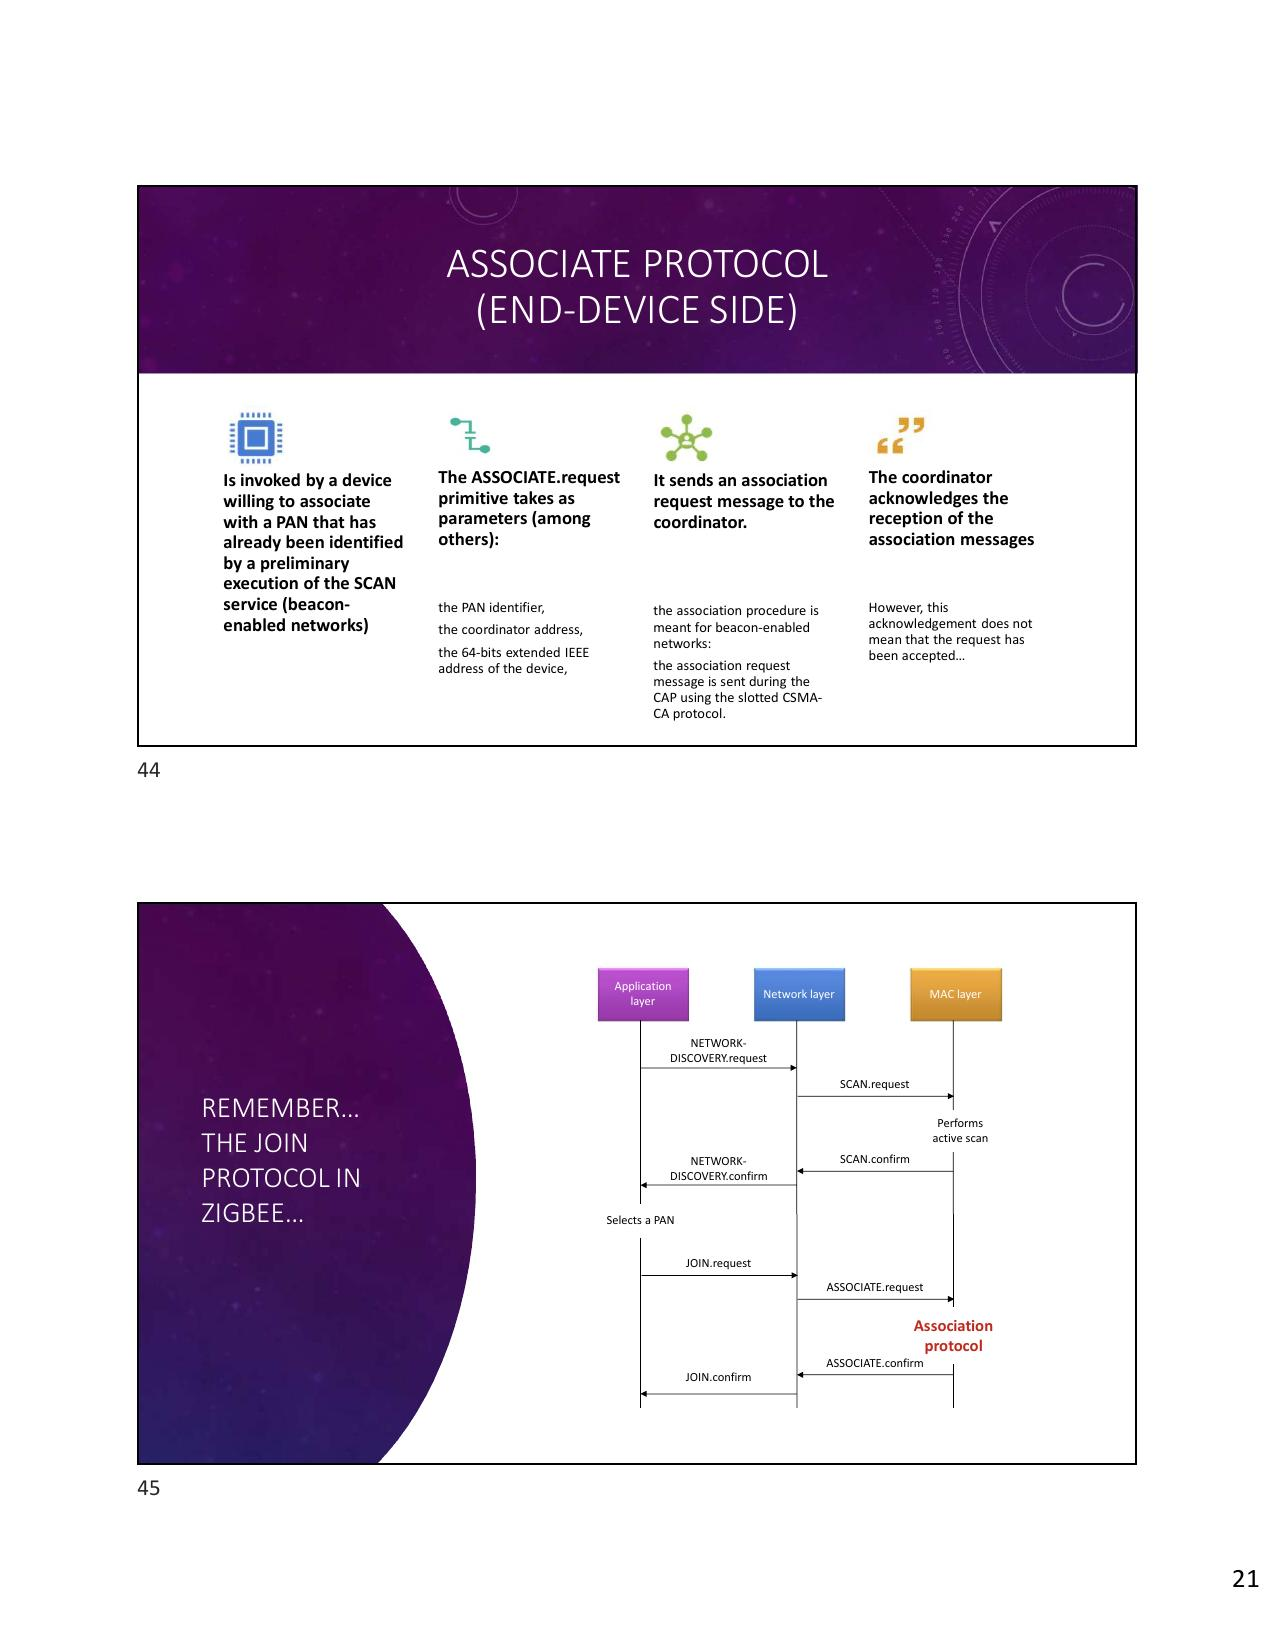
\includegraphics[keepaspectratio]{images/lezione-18-the-ieee-802-15-4-standard-img-05.jpg}}
\caption{In alto: lato end-device del protocollo ASSOCIATE con i passi
della primitiva ASSOCIATE.request. In basso: come il Join Protocol di
ZigBee (NWK layer) si appoggia al SCAN + ASSOCIATE del MAC 802.15.4.}
\end{figure}

\subsection{Management Service}\label{management-service}

Il \textbf{Management Service} include le seguenti primitive principali:

{\def\LTcaptype{none} % do not increment counter
\begin{longtable}[]{@{}
  >{\raggedright\arraybackslash}p{(\linewidth - 2\tabcolsep) * \real{0.5000}}
  >{\raggedright\arraybackslash}p{(\linewidth - 2\tabcolsep) * \real{0.5000}}@{}}
\toprule\noalign{}
\begin{minipage}[b]{\linewidth}\raggedright
Primitiva
\end{minipage} & \begin{minipage}[b]{\linewidth}\raggedright
Funzionalità
\end{minipage} \\
\midrule\noalign{}
\endhead
\bottomrule\noalign{}
\endlastfoot
ASSOCIATE & Richiesta di associazione di un nuovo dispositivo a una
PAN \\
DISASSOCIATE & Abbandono di una PAN \\
BEACON-NOTIFY & Fornisce al network layer il beacon ricevuto \\
GET / SET & Lettura/scrittura dei parametri della MAC-PIB \\
GTS & Richiesta di un GTS al coordinatore \\
SCAN & Ricerca di PAN attive \\
COMM-STATUS & Notifica al network layer dello stato di una
transazione \\
START & Avvia una PAN e inizia a inviare beacon; usato anche per la
device discovery \\
POLL & Richiesta di messaggi pendenti al coordinatore \\
\end{longtable}
}

Le primitive marcate ``O'' nella specifica sono opzionali per gli RFD.

\begin{center}\rule{0.5\linewidth}{0.5pt}\end{center}

\section{Protocollo di Associazione}\label{protocollo-di-associazione}

L'associazione è il processo con cui un dispositivo entra a far parte di
una PAN. È pensata per reti beacon-enabled e si compone di una fase sul
lato end-device e una sul lato coordinatore.

\subsection{Lato End-Device}\label{lato-end-device}

Il dispositivo che vuole associarsi deve aver identificato in anticipo
la PAN di destinazione attraverso il servizio \textbf{SCAN} (scansione
attiva). Invoca poi la primitiva \textbf{ASSOCIATE.request}, che prende
come parametri l'identificatore di PAN, l'indirizzo del coordinatore e
il proprio indirizzo IEEE a 64 bit esteso. La richiesta viene inviata
nel CAP usando CSMA-CA a slot. Il coordinatore invia un ACK immediato
--- ma questo non implica che la richiesta sia stata accettata.

\begin{calloutnote}{Connessione con ZigBee}

Il protocollo di JOIN dello stack ZigBee si appoggia esattamente a SCAN
+ ASSOCIATE del MAC 802.15.4: il NWK layer invoca
NETWORK-DISCOVERY.request → il MAC esegue SCAN → il NWK seleziona una
PAN → invoca JOIN.request → il MAC esegue il protocollo ASSOCIATE.

\end{calloutnote}

\subsection{Lato Coordinatore}\label{lato-coordinatore}

Dopo aver ricevuto la richiesta, il MAC layer del coordinatore emette
\textbf{ASSOCIATE.indication} verso il network layer (NWK), che decide
se accettare o rifiutare. In caso di accettazione, il NWK layer:

\begin{enumerate}
\def\labelenumi{\arabic{enumi}.}
\tightlist
\item
  Seleziona un \textbf{indirizzo a 16 bit} che il dispositivo utilizzerà
  in futuro al posto dell'indirizzo a 64 bit.
\item
  Invoca \textbf{ASSOCIATE.response}, passando come parametri
  l'indirizzo a 64 bit del dispositivo, il nuovo indirizzo a 16 bit e lo
  status della richiesta.
\item
  Il MAC layer invia la risposta di associazione usando
  \textbf{trasmissione indiretta} (il dispositivo deve fare polling per
  recuperarla).
\end{enumerate}

\begin{figure}
\centering
\pandocbounded{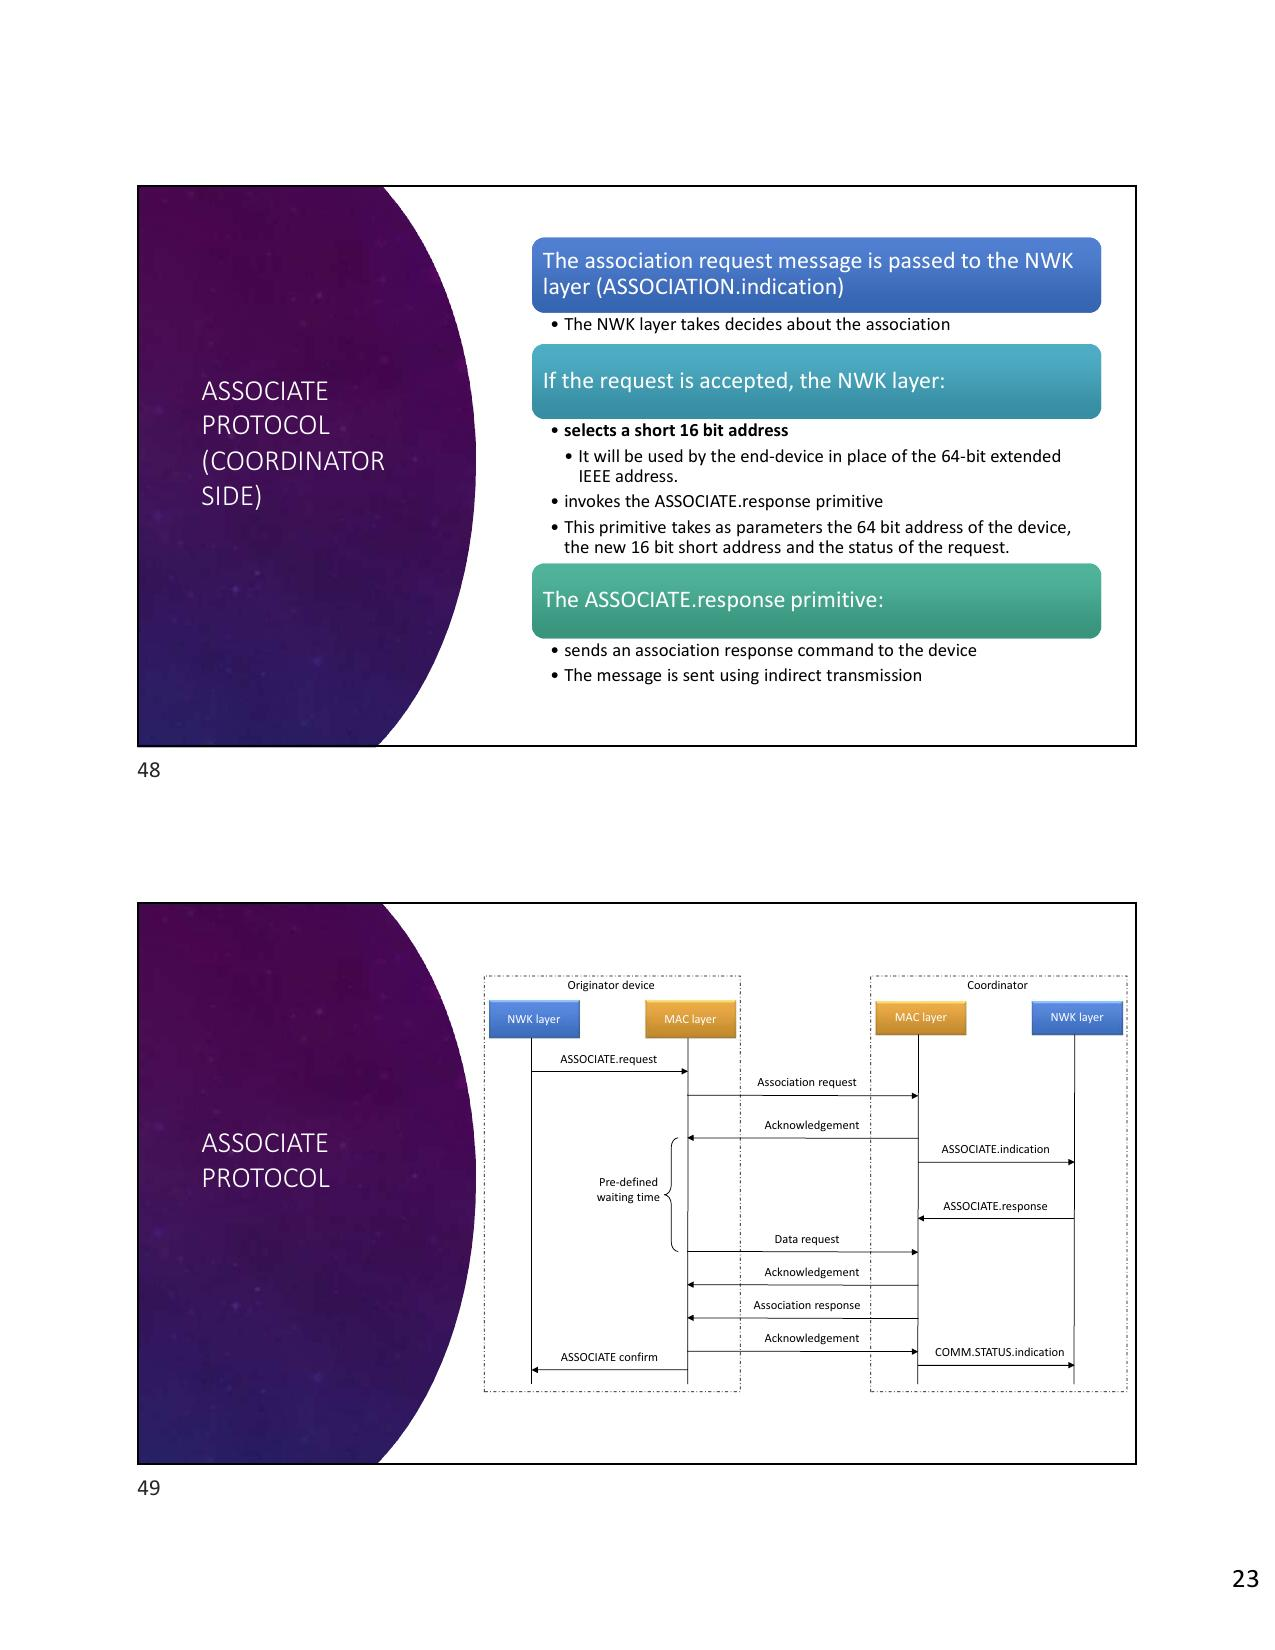
\includegraphics[keepaspectratio]{images/lezione-18-the-ieee-802-15-4-standard-img-06.jpg}}
\caption{Diagramma di sequenza completo del protocollo ASSOCIATE: flusso
tra NWK/MAC del dispositivo originatore e NWK/MAC del coordinatore. Dopo
il pre-defined waiting time, il dispositivo invia una Data request per
recuperare la risposta.}
\end{figure}

\subsection{Completamento del
Protocollo}\label{completamento-del-protocollo}

Dopo che il dispositivo ha recuperato la risposta (tramite Data request
→ ACK → Association response → ACK):

\begin{itemize}
\tightlist
\item
  Il \textbf{MAC layer dell'end-device} emette
  \textbf{ASSOCIATE.confirm} al NWK layer.
\item
  Il \textbf{MAC layer del coordinatore} emette
  \textbf{COMM-STATUS.Indication} al NWK layer, segnalando che
  l'associazione è conclusa --- con successo o con un codice di errore.
\end{itemize}

\begin{center}\rule{0.5\linewidth}{0.5pt}\end{center}

\section{Sicurezza del MAC Layer}\label{sicurezza-del-mac-layer}

IEEE 802.15.4 fornisce un supporto di base alla sicurezza direttamente
nel MAC layer. Le funzionalità avanzate --- come la gestione delle
chiavi e l'autenticazione dei dispositivi --- sono delegate ai layer
superiori. I servizi di sicurezza sono opzionali. Tutti i servizi di
sicurezza si basano su \textbf{crittografia simmetrica}; le chiavi
crittografiche sono fornite dai layer superiori.

\subsection{Controllo degli Accessi}\label{controllo-degli-accessi}

Ogni dispositivo mantiene un \textbf{ACL} (\emph{Access Control List})
che elenca i dispositivi con cui può comunicare. I frame ricevuti da
dispositivi non presenti nell'ACL vengono scartati.

\subsection{Cifratura dei Dati}\label{cifratura-dei-dati}

La cifratura simmetrica si applica ai dati, ai comandi e ai payload dei
beacon. La chiave può essere:

\begin{itemize}
\tightlist
\item
  una \textbf{group key} condivisa da un gruppo di dispositivi;
\item
  una \textbf{link key} condivisa solo tra due peer specifici.
\end{itemize}

\subsection{Integrità dei Frame}\label{integrituxe0-dei-frame}

L'integrità protegge i frame da modifiche non autorizzate e garantisce
che il frame provenga da un dispositivo in possesso della chiave
crittografica. Usa la stessa chiave della cifratura e si applica a frame
dati, beacon e comandi.

\subsection{Freschezza Sequenziale}\label{freschezza-sequenziale}

La \textbf{Sequential Freshness} ordina la sequenza dei frame in
ingresso per garantire che ogni frame ricevuto sia più recente
dell'ultimo frame ricevuto --- difesa contro gli attacchi di replay.

\begin{calloutnote}{Sintesi della Lezione}

IEEE 802.15.4 specifica il physical layer e il MAC layer per reti
LR-WPAN. Il physical layer opera su tre bande di frequenza (868 MHz, 902
MHz, 2.4 GHz), con eccellenti prestazioni in ambienti a basso SNR. Il
MAC layer distingue due tipi di dispositivi (RFD e FFD), supporta
topologie a stella e peer-to-peer, e gestisce l'accesso al canale con o
senza superframe. Il superframe è diviso in CAP (accesso CSMA-CA) e CFP
opzionale (GTS deterministici). Il protocollo di associazione permette
ai dispositivi di unirsi a una PAN esistente. La sicurezza di base ---
cifratura simmetrica, controllo accessi, integrità, freschezza --- è
integrata nel MAC layer.

\end{calloutnote}

\newpage

\chapter{Case Study: Biologging e Activity
Recognition}\label{case-study-biologging-e-activity-recognition}

Il biologging rappresenta uno dei casi d'uso più concreti e affascinanti
dell'IoT applicato al mondo naturale. La lezione sviluppa questo tema
attraverso un caso di studio reale: il progetto \textbf{Tortoise@}, che
automatizza il rilevamento delle attività di nidificazione delle
tartarughe con tecniche di machine learning embedded su dispositivi a
bassa potenza.

\begin{center}\rule{0.5\linewidth}{0.5pt}\end{center}

\section{Dal monitoraggio diretto al monitoraggio
sensoriale}\label{dal-monitoraggio-diretto-al-monitoraggio-sensoriale}

L'osservazione diretta degli animali (e degli esseri umani) è uno
strumento efficace per raccogliere informazioni sulle loro attività, ma
è per sua natura limitata: richiede la presenza fisica di un
osservatore, non può essere continua e copre solo una frazione ridotta
della vita del soggetto. L'impiego di sensori miniaturizzati ---
accelerometri, GPS, sensori di pressione, luce, temperatura ---
trasforma questa limitazione: il monitoraggio diventa \textbf{continuo},
\textbf{automatizzato} e capace di coprire quasi tutti gli aspetti della
vita del soggetto.

I dispositivi vengono fisicamente applicati agli animali in libertà
(\emph{free-range animals}). A questo punto si apre una distinzione
fondamentale tra due approcci:

\begin{calloutdefinition}{Biotelemetria vs Bio-logging}

\textbf{Biotelemetria}: i dati raccolti dai sensori vengono trasmessi in
tempo reale a una stazione remota tramite un'interfaccia wireless. Non
c'è memorizzazione locale.

\textbf{Bio-logging}: i dati vengono memorizzati nella memoria interna
del dispositivo. Il ricercatore deve fisicamente recuperare il
dispositivo per accedere ai dati. I dispositivi più moderni possono
anche trasmettere remotamente quando le condizioni lo permettono.

\end{calloutdefinition}

Il terzo elemento del quadro è l'\textbf{activity recognition}
(\emph{riconoscimento dell'attività}): un sistema che, a partire dai
segnali registrati durante l'attività dell'animale, riconosce
automaticamente le azioni compiute. Questo trasforma dati grezzi in
informazioni semanticamente ricche.

\section{Pipeline del Biologging}\label{pipeline-del-biologging}

Il flusso completo del biologging si articola in tre fasi: raccolta dei
dati → elaborazione dei dati → classificazione dell'attività.

\begin{figure}
\centering
\pandocbounded{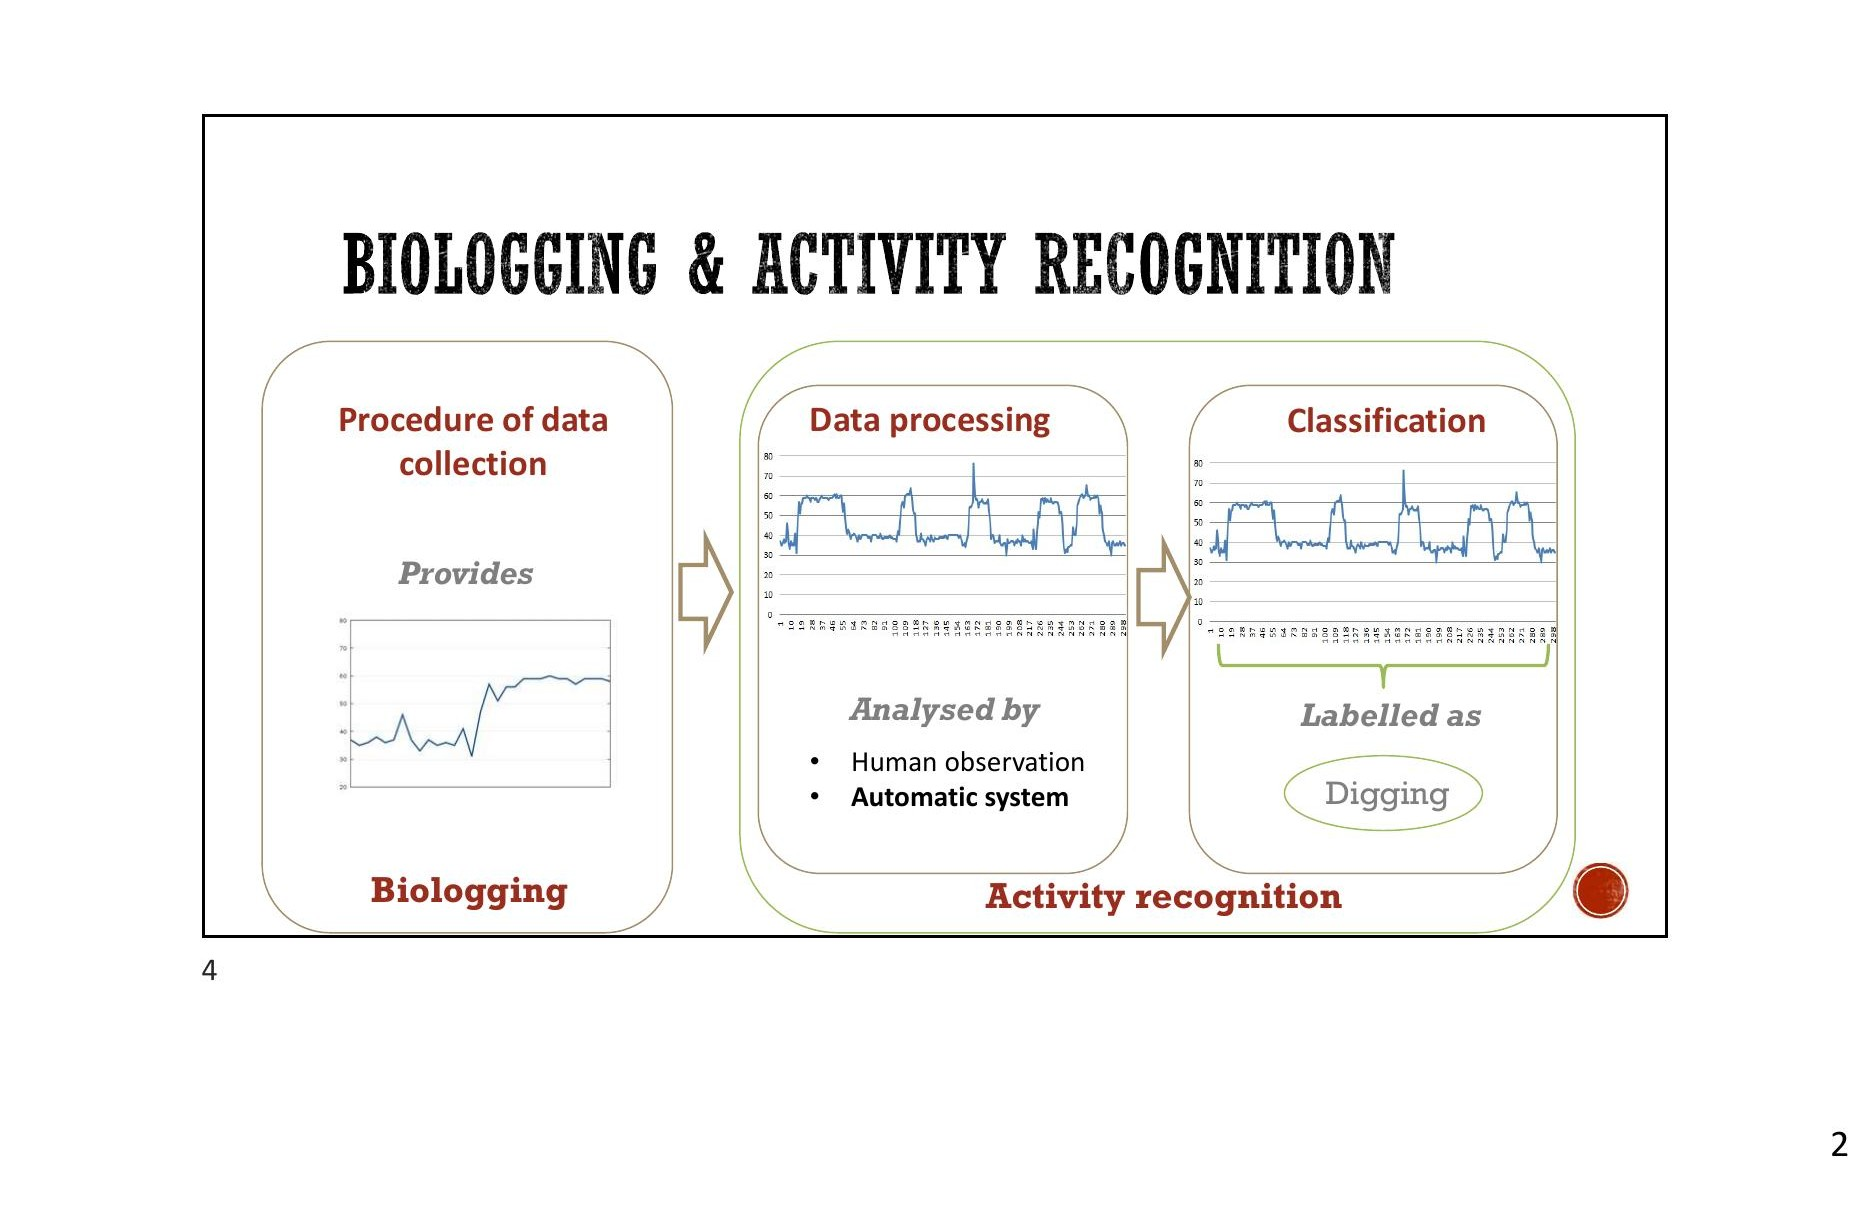
\includegraphics[keepaspectratio]{images/lezione-19-caso-studio-tartarughe-img-01.jpg}}
\caption{Il flusso completo: il dispositivo di biologging fornisce serie
temporali, che vengono analizzate (da un osservatore umano o da un
sistema automatico) e infine classificate in attività specifiche (es.
``digging'').}
\end{figure}

\begin{center}\rule{0.5\linewidth}{0.5pt}\end{center}

\section{Punti di forza e debolezza}\label{punti-di-forza-e-debolezza}

L'approccio sensoriale ha vantaggi importanti rispetto all'osservazione
tradizionale, ma introduce anche nuove sfide operative.

{\def\LTcaptype{none} % do not increment counter
\begin{longtable}[]{@{}
  >{\raggedright\arraybackslash}p{(\linewidth - 2\tabcolsep) * \real{0.5000}}
  >{\raggedright\arraybackslash}p{(\linewidth - 2\tabcolsep) * \real{0.5000}}@{}}
\toprule\noalign{}
\begin{minipage}[b]{\linewidth}\raggedright
Punti di forza
\end{minipage} & \begin{minipage}[b]{\linewidth}\raggedright
Debolezze
\end{minipage} \\
\midrule\noalign{}
\endhead
\bottomrule\noalign{}
\endlastfoot
Osservazioni puntuali tramite sensori & È necessario applicare il
dispositivo al soggetto \\
Funziona in ambienti domestici e selvatici & Necessità di recuperare
fisicamente il dispositivo \\
Enorme quantità di dati (serie temporali) & Quando la memoria si riempie
o la batteria si esaurisce, i dati vengono persi \\
--- & Vita limitata del dispositivo in monitoraggi intensivi \\
--- & Spesso solo analisi off-line \\
\end{longtable}
}

\begin{calloutwarning}{Il problema della durata della batteria}

Nei dispositivi di biologging, il consumo energetico è il vincolo
progettuale più critico. Un monitoraggio continuo che raccoglie e
trasmette serie temporali grezze porta rapidamente all'esaurimento della
batteria, limitando la durata utile del dispositivo a periodi ben
inferiori alle stagioni di osservazione necessarie.

\end{calloutwarning}

\begin{center}\rule{0.5\linewidth}{0.5pt}\end{center}

\section{Prospettiva del dispositivo: approccio convenzionale vs
approccio
innovativo}\label{prospettiva-del-dispositivo-approccio-convenzionale-vs-approccio-innovativo}

\subsection{Approccio convenzionale}\label{approccio-convenzionale}

Nel paradigma classico, il dispositivo è un semplice \emph{data logger}
a bassa potenza: raccoglie enormi quantità di dati di serie temporali e
deve poi o trasmetterli a una stazione remota o essere fisicamente
recuperato. Entrambe le opzioni hanno costi alti:

\begin{itemize}
\tightlist
\item
  \textbf{Comunicare} le serie temporali grezze è estremamente oneroso
  dal punto di vista energetico
\item
  \textbf{Recuperare} fisicamente il dispositivo è altamente invasivo
  per l'animale e per l'ecosistema
\end{itemize}

\subsection{Approccio innovativo: on-board
intelligence}\label{approccio-innovativo-on-board-intelligence}

\begin{figure}
\centering
\pandocbounded{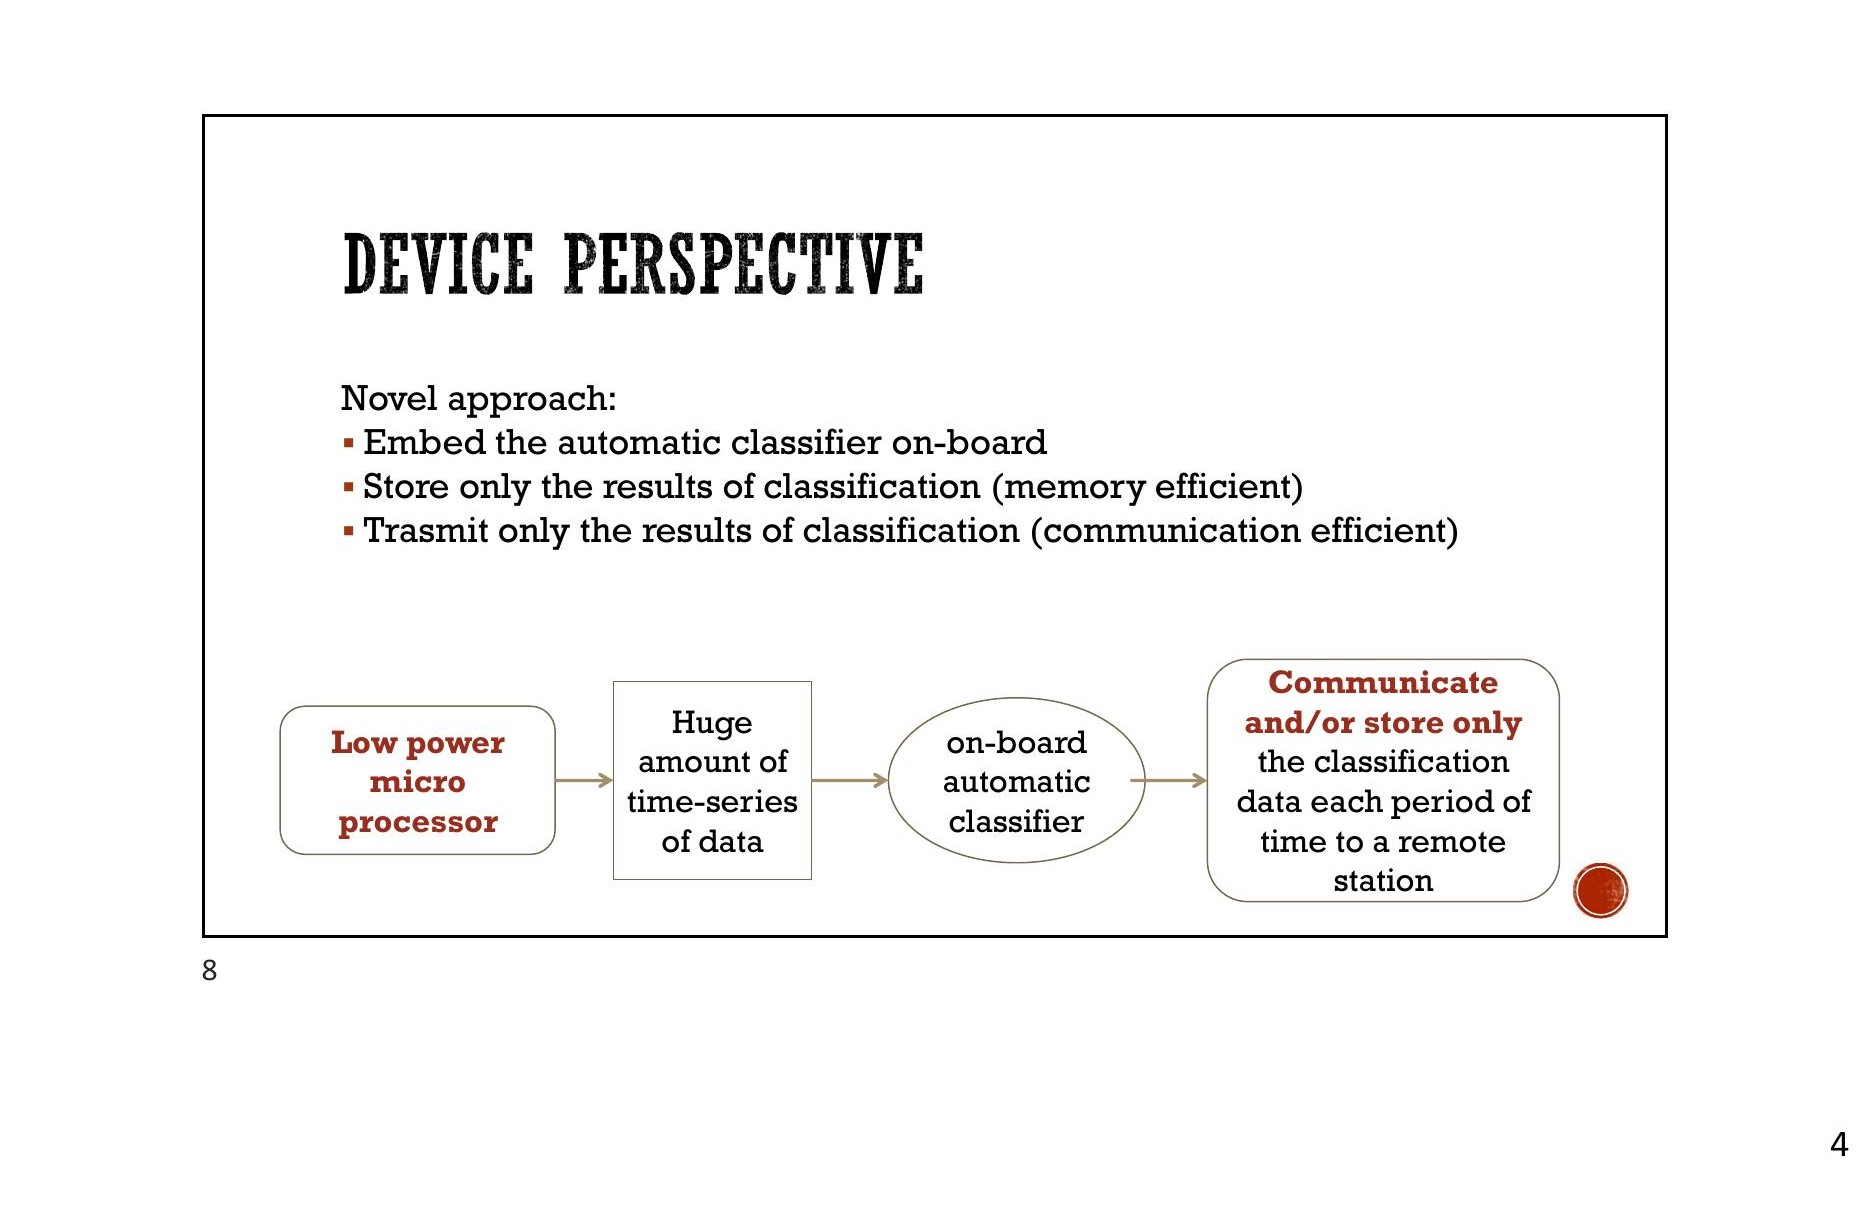
\includegraphics[keepaspectratio]{images/lezione-19-caso-studio-tartarughe-img-02.jpg}}
\caption{Il nuovo paradigma: un micro-processore a bassa potenza
incorpora un classificatore automatico. Invece delle serie temporali
grezze, vengono memorizzati e trasmessi solo i risultati della
classificazione, riducendo drasticamente il traffico dati e il consumo
energetico.}
\end{figure}

L'idea chiave è \textbf{spostare l'elaborazione sul dispositivo stesso}:

\begin{enumerate}
\def\labelenumi{\arabic{enumi}.}
\tightlist
\item
  Incorporare il classificatore automatico direttamente nel dispositivo
  (\emph{on-board})
\item
  Memorizzare solo i risultati della classificazione (efficienza di
  memoria)
\item
  Trasmettere solo i risultati della classificazione (efficienza di
  comunicazione)
\end{enumerate}

Questo approccio richiede classificatori leggeri, capaci di girare su
microcontrollori con risorse molto limitate, ma porta a vantaggi enormi
in termini di autonomia e invasività.

\begin{center}\rule{0.5\linewidth}{0.5pt}\end{center}

\section{Caso di studio: Tortoise@}\label{caso-di-studio-tortoise}

Il progetto di riferimento è:

\begin{quote}
Barbuti R., Chessa S., Micheli A., and Pucci R.; \emph{``Localizing
tortoise nests by neural networks''}; PloS One 2016.
\end{quote}

\subsection{Il problema}\label{il-problema}

I programmi di protezione delle tartarughe mirano a raccogliere le uova
e portarle in centri protetti, dove i piccoli vengono custoditi durante
il periodo più vulnerabile. Il problema è che \textbf{identificare i
nidi in natura è estremamente difficile}: le tartarughe sono molto abili
nel nasconderli. Il progetto \textbf{Tortoise@} automatizza questo
processo riconoscendo in tempo reale l'attività di scavo e comunicando
la posizione GPS agli erpetologi.

\begin{callouttip}{Perché il riconoscimento dell’attività funziona}

Le tartarughe scavano i nidi con le zampe posteriori. Questo
comportamento produce un pattern caratteristico nel segnale
dell'accelerometro, distinguibile dall'attività di camminata o di
alimentazione. La chiave è che lo scavo lascia una firma temporale
riconoscibile --- e questa firma può essere appresa da un modello di ML.

\end{callouttip}

\subsection{Idea del sistema}\label{idea-del-sistema}

\begin{figure}
\centering
\pandocbounded{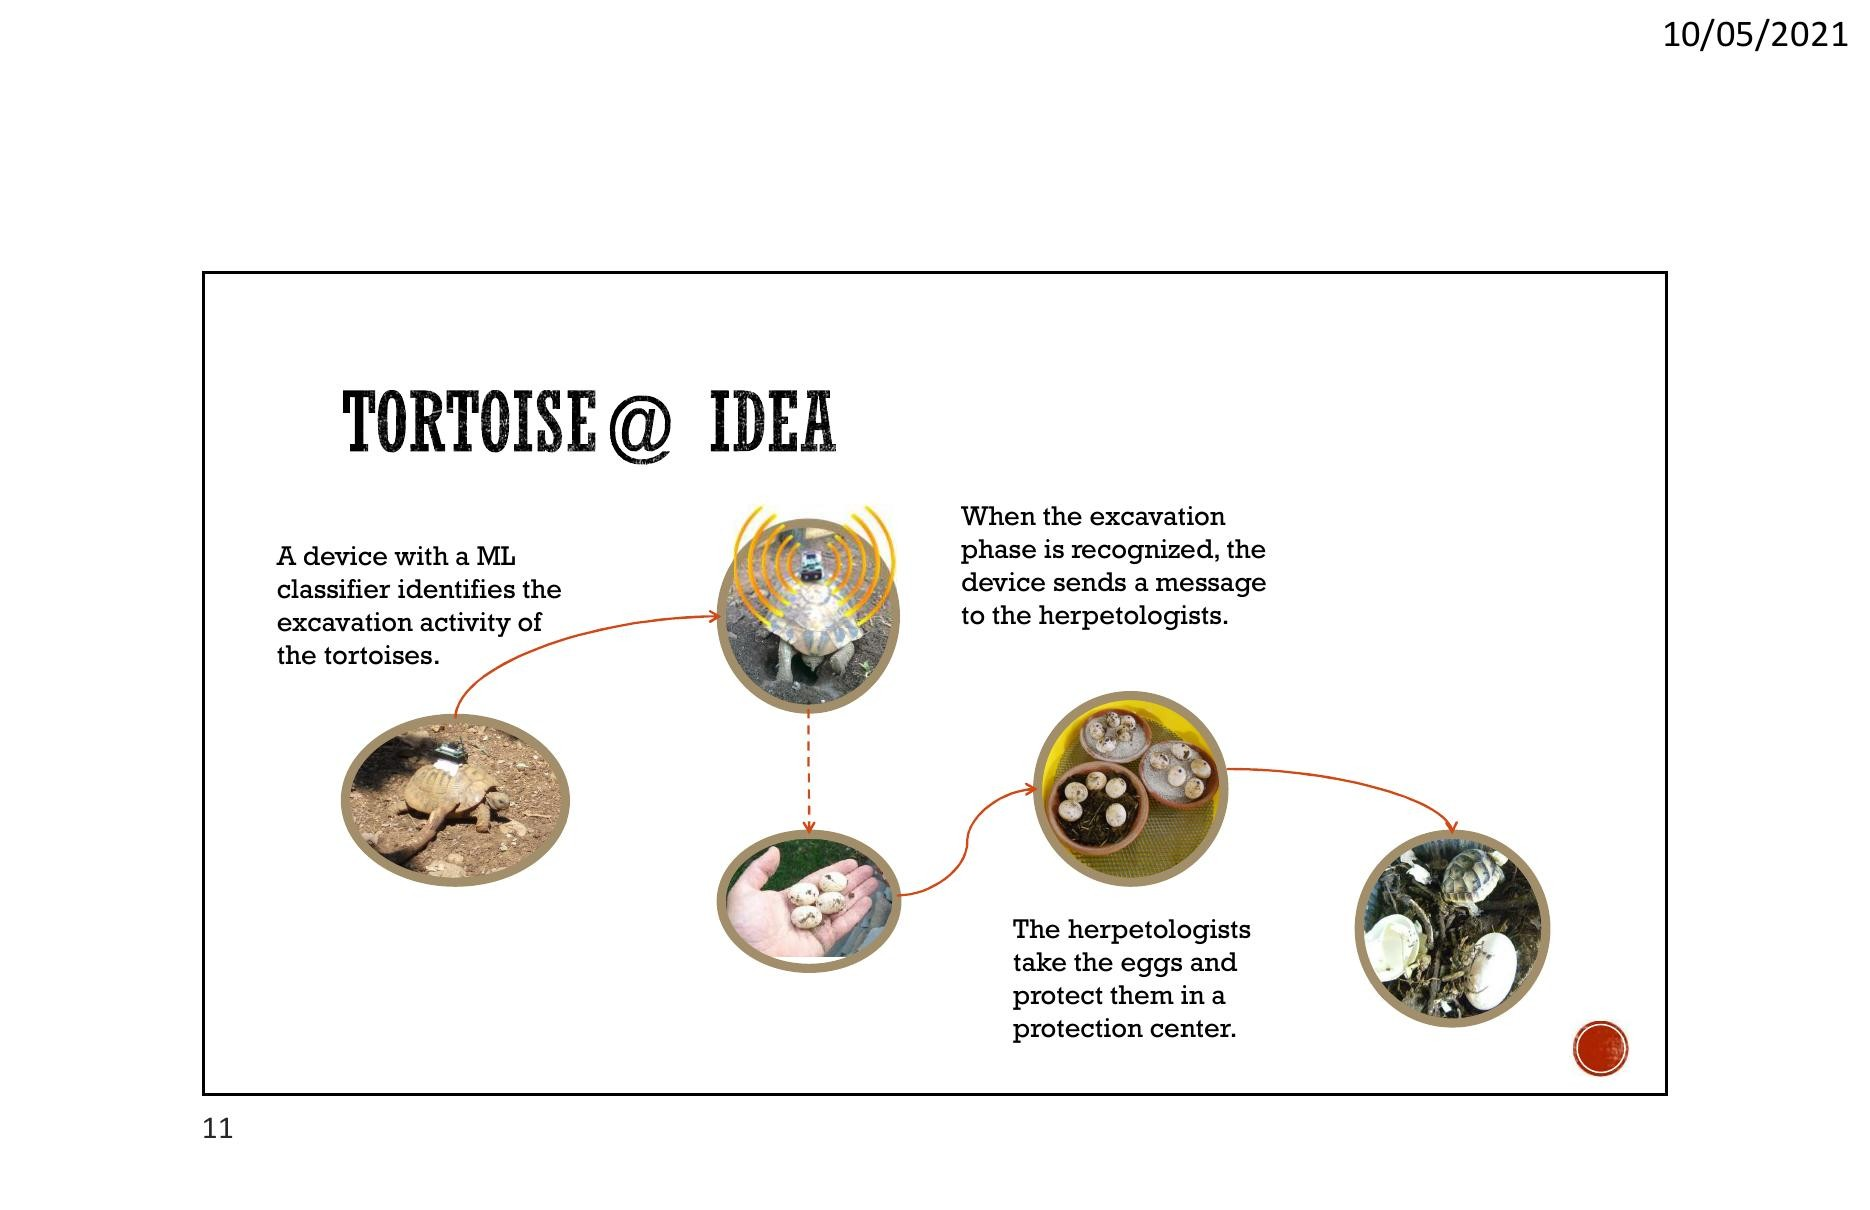
\includegraphics[keepaspectratio]{images/lezione-19-caso-studio-tartarughe-img-03.jpg}}
\caption{Il sistema Tortoise@: un dispositivo con classificatore ML
identifica l'attività di scavo, invia un messaggio agli erpetologi che
recuperano le uova e le portano in un centro di protezione.}
\end{figure}

\subsection{Vincoli biologici e scelte
progettuali}\label{vincoli-biologici-e-scelte-progettuali}

La biologia delle tartarughe guida direttamente le scelte
ingegneristiche:

\begin{itemize}
\tightlist
\item
  Le tartarughe depongono le uova in primavera, in un periodo di circa
  \textbf{4 mesi}
\item
  Una singola tartaruga può deporre più volte (generalmente 3-4 volte)
\item
  La nidificazione avviene di giorno, in luoghi caldi e ben illuminati
\item
  La nidificazione dura \textbf{più di un'ora}
\item
  Le tartarughe scavano il nido con le zampe posteriori
\end{itemize}

Da queste osservazioni derivano direttamente i requisiti tecnici:

\begin{itemize}
\tightlist
\item
  Il dispositivo deve durare \textbf{almeno 4 mesi}
\item
  L'attività di scavo è rilevabile con gli accelerometri
\item
  I sensori ambientali (luce e temperatura) possono limitare l'uso degli
  accelerometri ai soli momenti potenzialmente rilevanti
\end{itemize}

\subsection{Architettura per l'efficienza
energetica}\label{architettura-per-lefficienza-energetica}

\begin{figure}
\centering
\pandocbounded{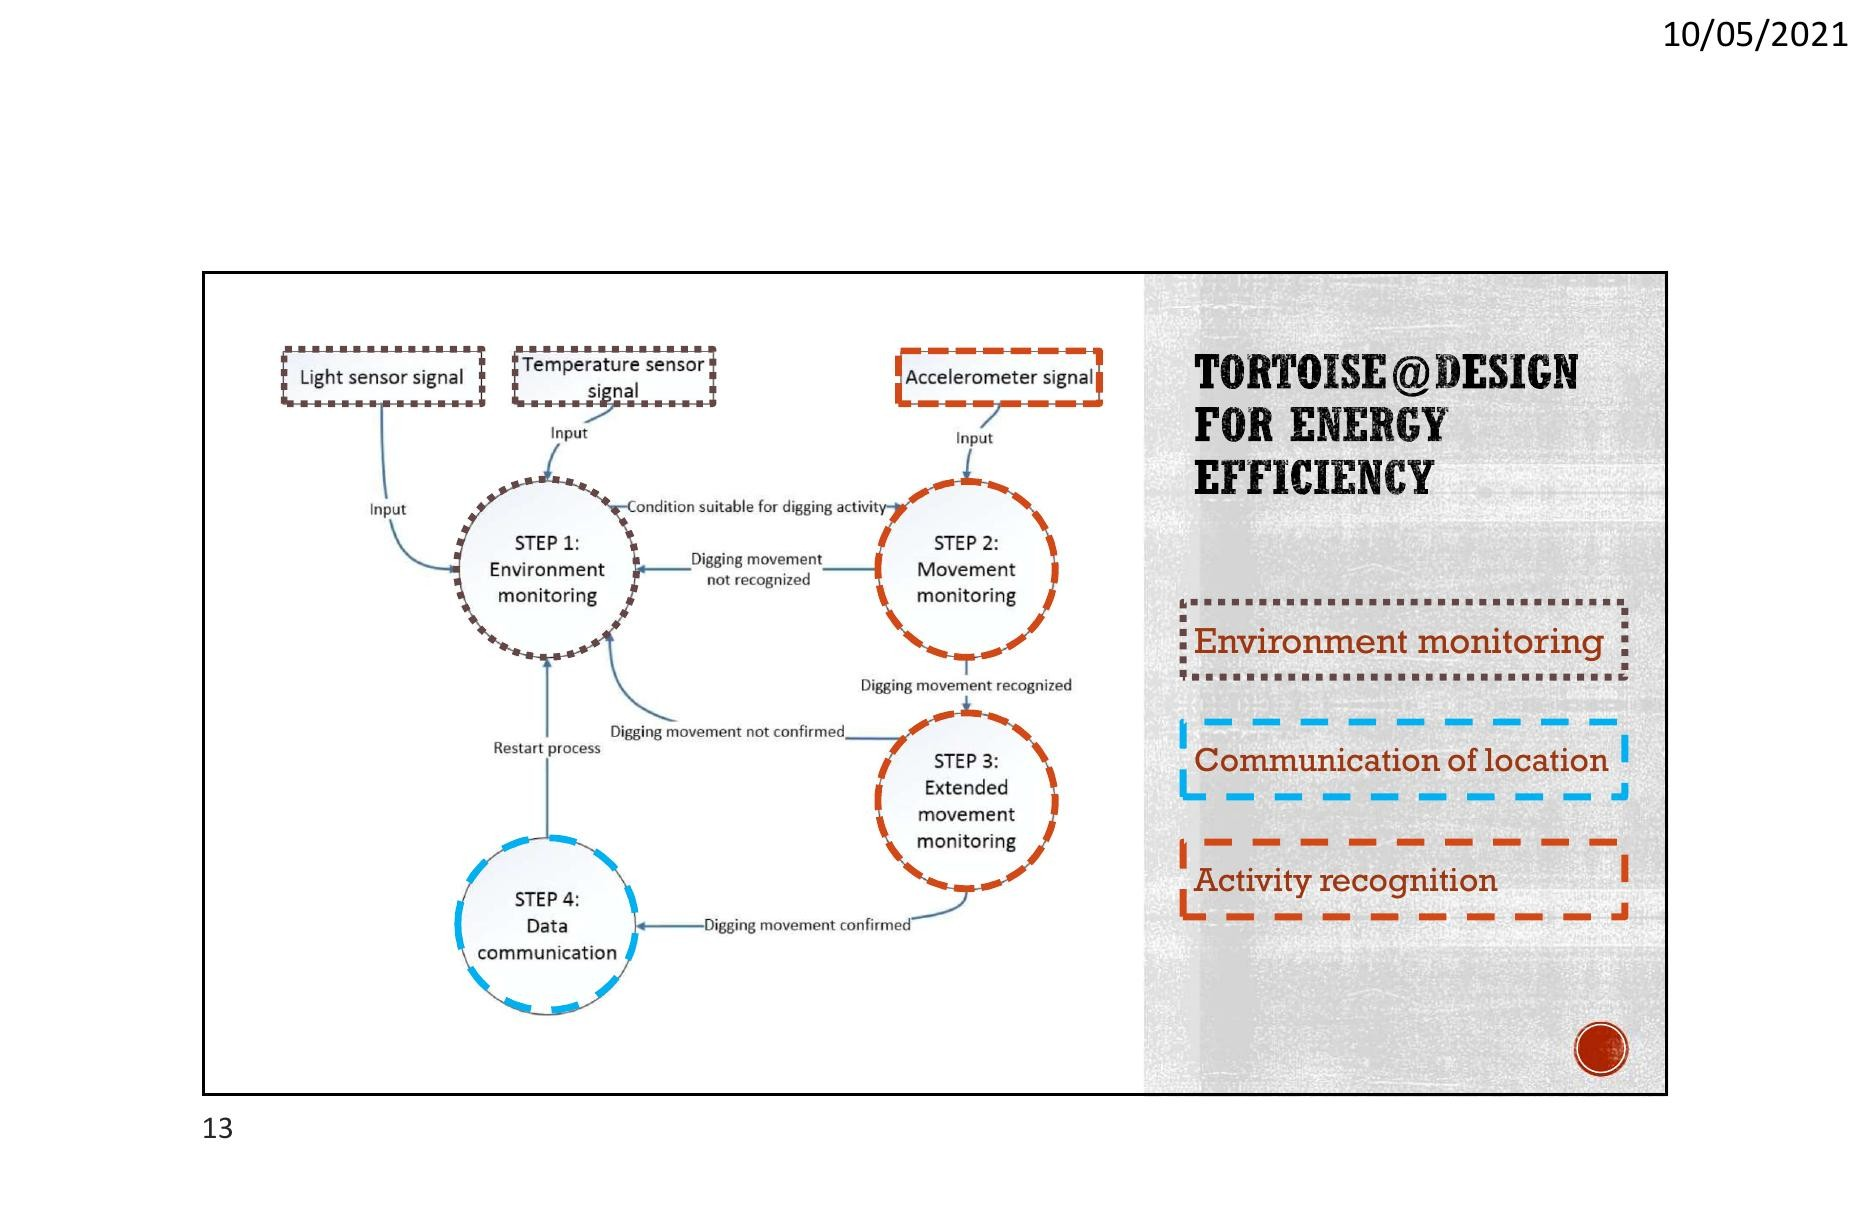
\includegraphics[keepaspectratio]{images/lezione-19-caso-studio-tartarughe-img-04.jpg}}
\caption{Il design di Tortoise@ per l'efficienza energetica: la macchina
a stati usa sensori ambientali a bassa frequenza come gate per attivare
il campionamento dell'accelerometro, minimizzando il consumo
complessivo.}
\end{figure}

La logica di controllo del dispositivo è progettata per minimizzare
l'uso dell'accelerometro (il sensore più energivoro):

\begin{enumerate}
\def\labelenumi{\arabic{enumi}.}
\tightlist
\item
  \textbf{Step 1 --- Environment monitoring}: i sensori ambientali (luce
  e temperatura) vengono campionati a frequenza molto bassa (0,01 Hz).
  Il campionamento notturno viene evitato completamente.
\item
  \textbf{Step 2 --- Movement monitoring}: solo quando le condizioni
  ambientali sono adatte si attiva il campionamento dell'accelerometro a
  1 Hz per 5 minuti.
\item
  \textbf{Step 3 --- Extended movement monitoring}: se la risposta è
  negativa, il dispositivo sospende per almeno mezz'ora (lo scavo dura
  almeno un'ora, quindi non si perde nessun evento rilevante).
\item
  \textbf{Step 4 --- Data communication}: se il classificatore è certo
  che la tartaruga stia scavando, trasmette la posizione GPS. Per
  confermare, il ciclo di campionamento viene ripetuto 3 volte,
  riducendo i falsi positivi. La trasmissione radio avviene solo poche
  volte nell'arco di diversi mesi.
\end{enumerate}

\begin{calloutnote}{Efficienza di sistema}

Questo design a cascata è un esempio di \textbf{duty cycling
intelligente}: invece di campionare continuamente, si usa un sensore
economico (luce/temperatura) come trigger per attivare il sensore
costoso (accelerometro). Il risultato è un'autonomia molto più lunga
rispetto a un campionamento naïve.

\end{calloutnote}

\begin{center}\rule{0.5\linewidth}{0.5pt}\end{center}

\section{Dataset e classificazione}\label{dataset-e-classificazione}

\subsection{Raccolta dati}\label{raccolta-dati}

Il dataset è stato raccolto presso il «Centro di protezione tartarughe
Mediterranee» di Massa Marittima, Italia. Gli animali coinvolti sono
femmine adulte di \emph{Testudo hermanni}, \emph{Testudo graeca} e
\emph{Testudo marginata}. Le attività registrate sono tre:
\textbf{digging} (scavo), \textbf{eating} (alimentazione),
\textbf{walking} (camminata).

Il sensore utilizzato è un accelerometro a un asse (asse X) con un
dispositivo \textbf{MicaZ}, campionato a 1 Hz.

\begin{figure}
\centering
\pandocbounded{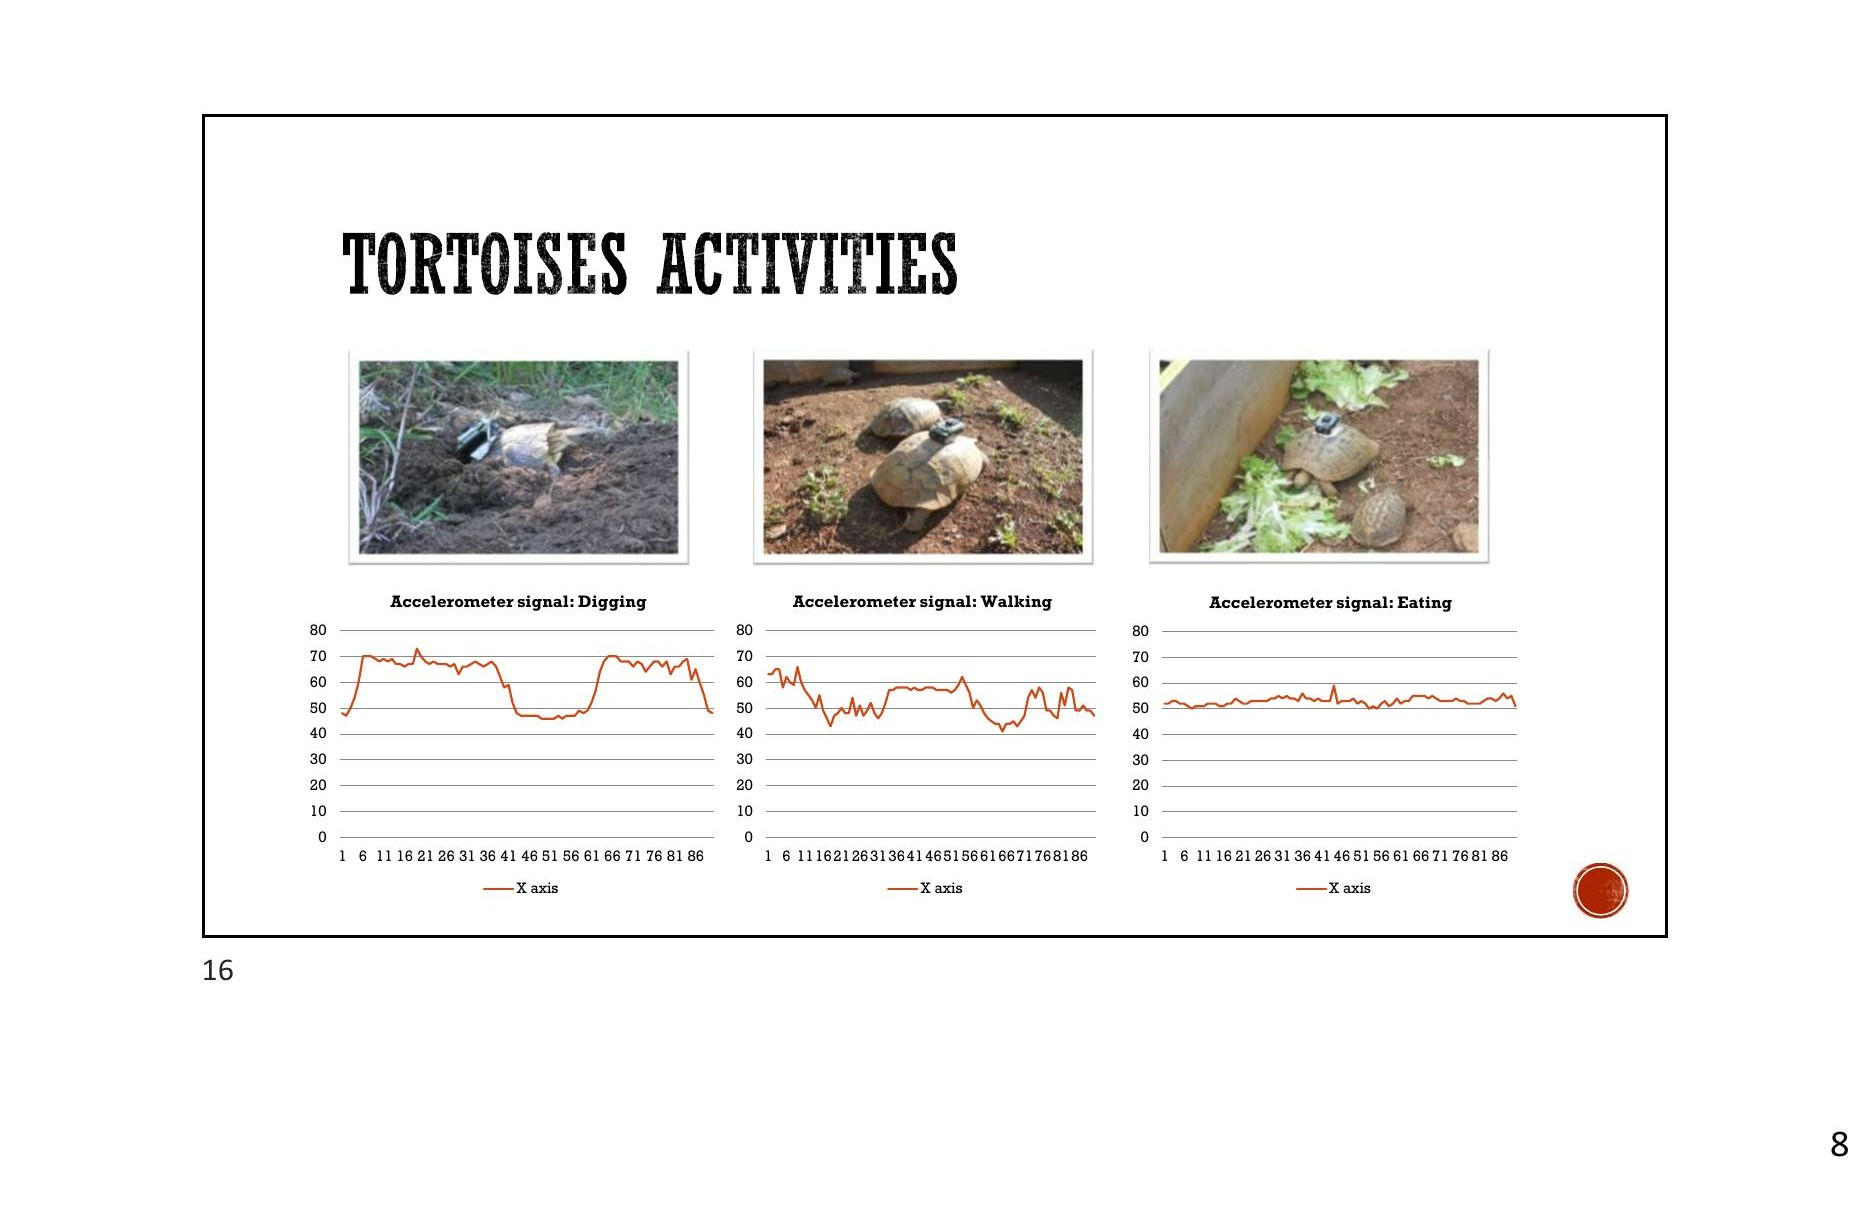
\includegraphics[keepaspectratio]{images/lezione-19-caso-studio-tartarughe-img-05.jpg}}
\caption{I segnali dell'accelerometro (asse X) per le tre attività: lo
scavo (digging) mostra un pattern oscillatorio caratteristico con
ampiezza maggiore e periodicità regolare rispetto alla camminata e
all'alimentazione.}
\end{figure}

\subsection{Struttura del dataset}\label{struttura-del-dataset}

Il dataset è organizzato in due strutture complementari:

\textbf{Sequences dataset} (task asincrono): - Sequenze di 300 secondi,
campionamento a 1 Hz - 126 sequenze totali con classificazione positiva
e negativa - 56 sequenze nel test set, le rimanenti per training e
validazione

\textbf{Patterns dataset} (task sincrono): - Sequenze di 90 secondi a 1
Hz - 67 pattern con classificazione positiva e 67 negativa per la
selezione del modello - 10 pattern positivi e 10 negativi per la
validazione

\begin{calloutnote}{Perché due granularità?}

La scelta della dimensione della finestra dipende dalla forma del
segnale di scavo. La finestra di 300 secondi (5 minuti) cattura
un'intera sequenza di scavo, mentre quella di 90 secondi è sufficiente a
riconoscere un \emph{pattern} caratteristico. Le finestre più piccole
abilitano la classificazione sincrona (in streaming), quelle più grandi
quella asincrona (per batch).

\end{calloutnote}

\subsection{Approcci di
classificazione}\label{approcci-di-classificazione}

Vengono valutati \textbf{SVM} (\emph{Support Vector Machine}) e diversi
modelli di reti neurali:

\begin{calloutdefinition}{Modelli considerati}

\begin{itemize}
\tightlist
\item
  \textbf{IDNN} (Input-Delay Neural Network): rete neurale feedforward
  con delay di input
\item
  \textbf{CNN} (Convolutional Neural Network): rete convoluzionale
\item
  \textbf{ESN} (Echo State Network): rete neurale ricorrente con
  reservoir fisso
\item
  \textbf{SVM}: classificatore a vettori di supporto
\end{itemize}

\end{calloutdefinition}

I due paradigmi di classificazione sono:

\textbf{Task asincrono}: classificazione di finestre singole (IDNN, CNN,
SVM, ESN). L'output della rete dipende dall'intera finestra.

\textbf{Task sincrono}: classificazione step-by-step su uno stream di
dati (solo ESN). L'output non richiede l'intera finestra; si basa sugli
ultimi 90 secondi di campioni.

\begin{center}\rule{0.5\linewidth}{0.5pt}\end{center}

\section{Risultati}\label{risultati}

\subsection{Task asincrono}\label{task-asincrono}

\begin{figure}
\centering
\pandocbounded{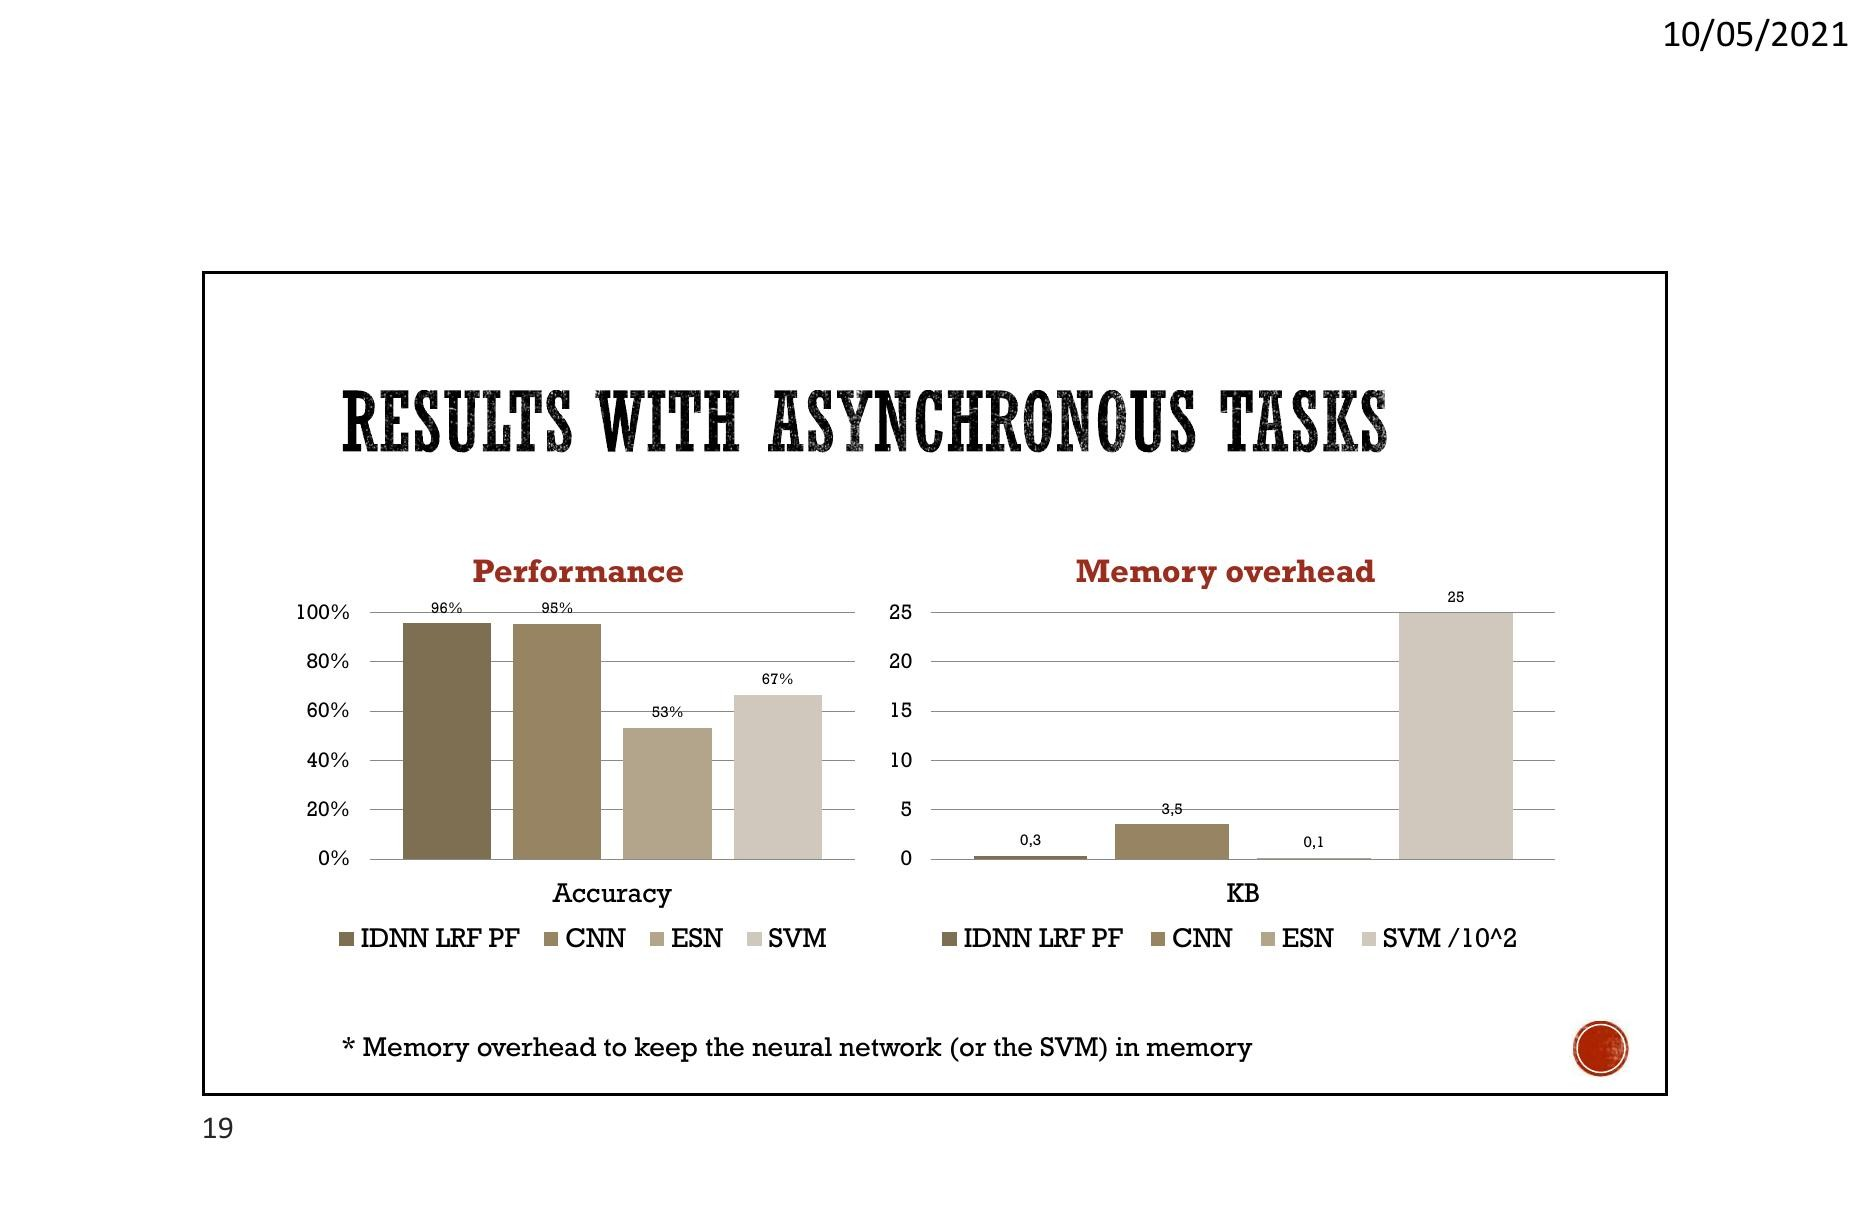
\includegraphics[keepaspectratio]{images/lezione-19-caso-studio-tartarughe-img-06.jpg}}
\caption{Confronto tra modelli per il task asincrono: accuratezza
(sinistra) e overhead di memoria per mantenere il modello in RAM
(destra). IDNN e CNN raggiungono \textasciitilde95\% di accuratezza, ma
con overhead molto diverso.}
\end{figure}

{\def\LTcaptype{none} % do not increment counter
\begin{longtable}[]{@{}lll@{}}
\toprule\noalign{}
Modello & Accuratezza & Overhead memoria \\
\midrule\noalign{}
\endhead
\bottomrule\noalign{}
\endlastfoot
IDNN LRF PF & \textasciitilde96\% & 0,3 KB \\
CNN & \textasciitilde95\% & 3,5 KB \\
ESN & \textasciitilde67\% & 0,1 KB \\
SVM & \textasciitilde53\% & 25 KB / 10² \\
\end{longtable}
}

\begin{callouttip}{Trade-off chiave}

IDNN e CNN raggiungono la stessa accuratezza (\textasciitilde95\%), ma
IDNN richiede solo \textbf{0,3 KB} contro i \textbf{3,5 KB} di CNN. Su
microcontrollori con pochi KB di RAM, questa differenza è determinante.
L'SVM, nonostante la sua semplicità concettuale, ha un overhead di
memoria molto alto a causa della necessità di memorizzare i vettori di
supporto.

\end{callouttip}

\subsection{Task sincrono (ESN)}\label{task-sincrono-esn}

\begin{figure}
\centering
\pandocbounded{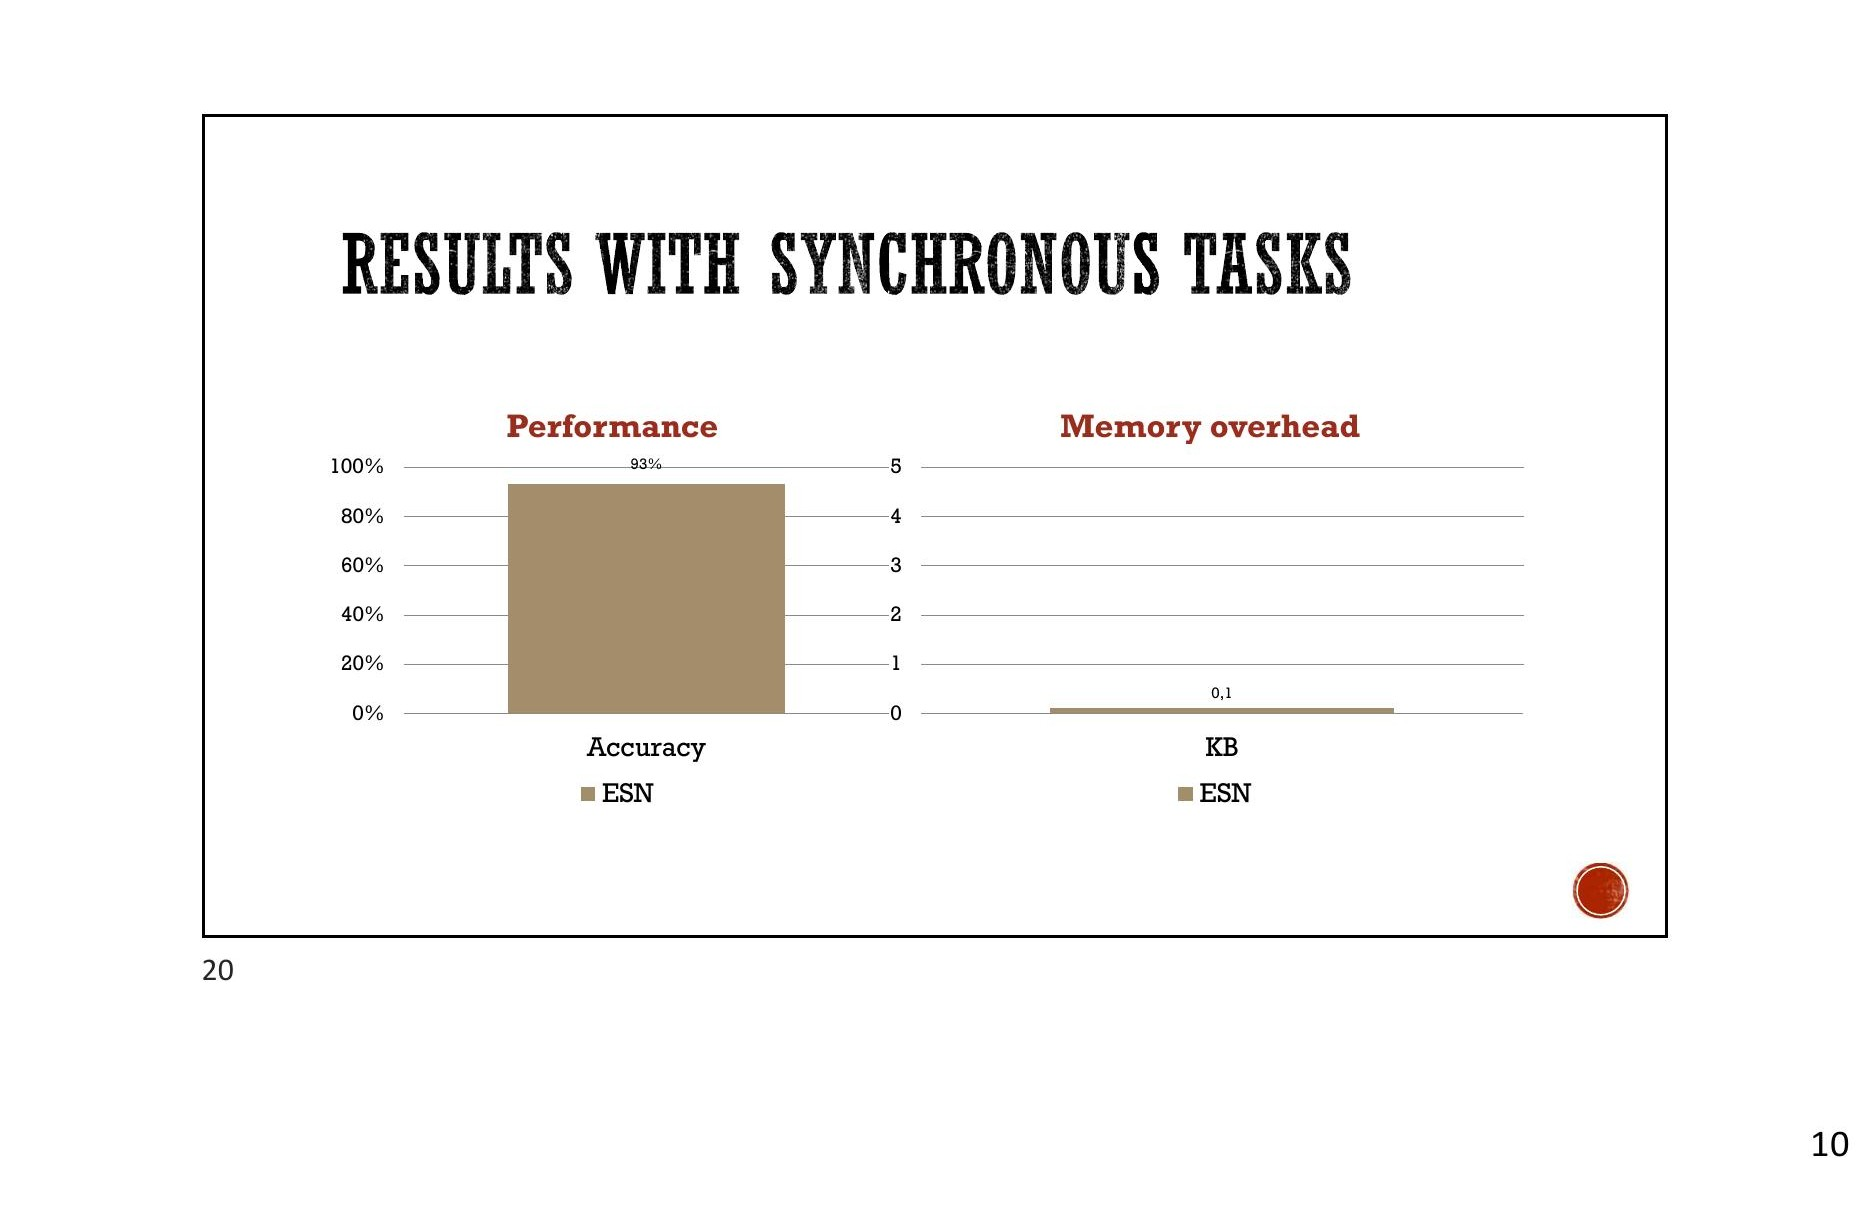
\includegraphics[keepaspectratio]{images/lezione-19-caso-studio-tartarughe-img-07.jpg}}
\caption{L'ESN nel task sincrono raggiunge il 93\% di accuratezza con
soli 0,1 KB di overhead --- risultato notevole per un modello in
streaming.}
\end{figure}

Il task sincrono con ESN è la \textbf{prima applicazione di ESN per il
riconoscimento di attività animali}. Il modello raggiunge il 93\% di
accuratezza con un overhead di soli 0,1 KB, adatto a microcontrollori
estremamente vincolati.

\begin{center}\rule{0.5\linewidth}{0.5pt}\end{center}

\section{Confronto cloud vs elaborazione
locale}\label{confronto-cloud-vs-elaborazione-locale}

La tabella seguente mostra il risparmio ottenibile spostando
l'elaborazione on-device rispetto all'approccio cloud-based tradizionale
(su un periodo di 4 mesi):

{\def\LTcaptype{none} % do not increment counter
\begin{longtable}[]{@{}
  >{\raggedright\arraybackslash}p{(\linewidth - 4\tabcolsep) * \real{0.3333}}
  >{\raggedright\arraybackslash}p{(\linewidth - 4\tabcolsep) * \real{0.3333}}
  >{\raggedright\arraybackslash}p{(\linewidth - 4\tabcolsep) * \real{0.3333}}@{}}
\toprule\noalign{}
\begin{minipage}[b]{\linewidth}\raggedright
\end{minipage} & \begin{minipage}[b]{\linewidth}\raggedright
Elaborazione cloud
\end{minipage} & \begin{minipage}[b]{\linewidth}\raggedright
Elaborazione locale
\end{minipage} \\
\midrule\noalign{}
\endhead
\bottomrule\noalign{}
\endlastfoot
Posizione GPS trasmessa & ogni mezz'ora (46 KB totali) & solo quando
rilevato scavo (poche volte) \\
Dati accelerometro & 13 MB (4 mesi a 1 Hz) & max 3 KB (una finestra
temporale) \\
Analisi & off-line dopo recupero & in tempo reale sul dispositivo \\
Invasività & alta (recupero fisico) & bassa (trasmissione radio rara) \\
\end{longtable}
}

\begin{calloutnote}{Sintesi del risparmio}

L'approccio locale riduce il dato memorizzato da \textbf{13 MB a 3 KB}
per l'accelerometro, e limita le trasmissioni GPS a \textbf{poche
eventi} in 4 mesi invece di una ogni 30 minuti. Questo si traduce
direttamente in una durata della batteria molto più lunga e in
un'invasività drasticamente ridotta.

\end{calloutnote}

\begin{center}\rule{0.5\linewidth}{0.5pt}\end{center}

\section{Strutture dati in memoria}\label{strutture-dati-in-memoria}

Il dispositivo utilizza due strutture dati:

\begin{enumerate}
\def\labelenumi{\arabic{enumi}.}
\tightlist
\item
  \textbf{Struttura per il modello}: memorizza i pesi della rete neurale
  o i vettori di supporto dell'SVM (0,1--3,5 KB a seconda del modello).
\item
  \textbf{Struttura per i campioni}: memorizza al massimo una finestra
  di \textbf{300 campioni} (nel caso peggiore), ovvero circa 3 KB a 10
  bit per campione. Con ESN, la finestra utile è di soli 90 campioni.
\end{enumerate}

\newpage

\chapter{Embedded Programming e
Arduino}\label{embedded-programming-e-arduino}

Gli \textbf{sistemi embedded} (\emph{embedded systems}) rappresentano
una categoria fondamentale nell'informatica moderna, specialmente nel
contesto dei sistemi cyber-fisici e dell'IoT. A differenza dei personal
computer, progettati per eseguire un insieme arbitrario e variabile di
applicazioni, un sistema embedded è costruito per svolgere \textbf{una
funzione dedicata e specifica}. Questa differenza non è solo funzionale
ma architetturale: hardware e software vengono progettati insieme in
parallelo, in quello che si chiama \textbf{co-design hardware-software}.

\section{Sistemi Embedded e
Microcontrollori}\label{sistemi-embedded-e-microcontrollori}

\begin{calloutdefinition}{Sistema Embedded}

Un sistema embedded è un sistema computazionale progettato per svolgere
una funzione dedicata. Hardware e software sono co-progettati, e il
sistema può includere anche componenti meccanici. Il cuore di un sistema
embedded è tipicamente un \textbf{microcontrollore}.

\end{calloutdefinition}

Il microcontrollore è un singolo chip che integra al suo interno un
microprocessore, memoria e interfacce di I/O. È ottimizzato per il
controllo di periferiche e interagisce con il dispositivo
elettromeccanico nel quale è ``embedded'' per fornire controllo. Proprio
per questo scopo di controllo, un sistema embedded ha spesso vincoli di
\textbf{real-time}: la correttezza temporale è importante quanto quella
funzionale.

I microcontrollori possono essere classificati in base alla loro
flessibilità:

{\def\LTcaptype{none} % do not increment counter
\begin{longtable}[]{@{}
  >{\raggedright\arraybackslash}p{(\linewidth - 4\tabcolsep) * \real{0.3333}}
  >{\raggedright\arraybackslash}p{(\linewidth - 4\tabcolsep) * \real{0.3333}}
  >{\raggedright\arraybackslash}p{(\linewidth - 4\tabcolsep) * \real{0.3333}}@{}}
\toprule\noalign{}
\begin{minipage}[b]{\linewidth}\raggedright
Tipo
\end{minipage} & \begin{minipage}[b]{\linewidth}\raggedright
Descrizione
\end{minipage} & \begin{minipage}[b]{\linewidth}\raggedright
Esempi
\end{minipage} \\
\midrule\noalign{}
\endhead
\bottomrule\noalign{}
\endlastfoot
General purpose & Adattabili a più applicazioni embedded & Arduino Uno
(ATmega328) \\
ASIC & \emph{Application-Specific Integrated Circuits}, progettati per
prodotti specifici & Chip in elettrodomestici \\
SoC & \emph{System on a Chip}, termine più ampio, include anche
processori per smartphone & Qualcomm Snapdragon \\
\end{longtable}
}

I microcontrollori sono usati in una vasta gamma di applicazioni:
allarmi, wearable, giocattoli, sensori industriali, e molte altre. Le
piattaforme più popolari per prototyping e didattica sono
\textbf{Arduino} e \textbf{Raspberry Pi}.

\begin{center}\rule{0.5\linewidth}{0.5pt}\end{center}

\section{Sfide della Programmazione su Sistemi
Embedded}\label{sfide-della-programmazione-su-sistemi-embedded}

Programmare per sistemi embedded introduce vincoli che non esistono
nello sviluppo software tradizionale. Comprendere queste sfide è
fondamentale per scrivere codice corretto ed efficiente.

\subsection{Risorse Hardware Limitate}\label{risorse-hardware-limitate}

La prima differenza rispetto ai PC tradizionali riguarda la memoria: un
tipico microcontrollore dispone di pochissima RAM (es. Arduino Uno ha
solo 2 KB di SRAM per i dati e 32 KB di memoria Flash per il programma).
Non esiste in genere un filesystem, e l'interfaccia utente è ridotta a
pochi LED o bottoni. In molti casi \textbf{non è presente un sistema
operativo} (sistemi \emph{bare-metal}): esiste una sola applicazione che
gestisce direttamente gli interrupt.

\subsection{Correttezza Temporale}\label{correttezza-temporale}

\begin{calloutwarning}{Real-Time è un requisito funzionale}

In molti sistemi embedded la correttezza temporale è parte integrante
dei requisiti funzionali, non solo una questione di prestazioni. Un
sistema GPS che identifica correttamente tutti i waypoint ma li segnala
in ritardo è \textbf{inutile}.

\end{calloutwarning}

\subsection{Alta Affidabilità}\label{alta-affidabilituxe0}

I sistemi embedded operano spesso in ambienti ostili o imprevedibili. Un
requisito comune è la disponibilità \emph{four nines} (99.99\%), che
corrisponde a non più di 9 secondi di downtime al giorno. Questo è
particolarmente difficile da garantire quando eventi ambientali
imprevedibili possono alterare la sequenza di esecuzione.

\subsection{Gestione Efficiente della
Memoria}\label{gestione-efficiente-della-memoria}

La memoria è costosa in termini economici e fisici. Un programmatore
embedded deve riuscire a far stare il proprio codice nello spazio
disponibile, il che richiede un approccio particolarmente creativo e
disciplinato.

\subsection{Power Management}\label{power-management}

In molti sistemi embedded, specialmente quelli alimentati a batteria, la
gestione dell'energia è critica. La capacità di entrare in uno stato di
basso consumo quando il sistema è inattivo è una caratteristica
imprescindibile.

\begin{center}\rule{0.5\linewidth}{0.5pt}\end{center}

\section{Sistemi Operativi per Sistemi
Embedded}\label{sistemi-operativi-per-sistemi-embedded}

Le funzionalità del sistema operativo variano enormemente in base alle
capacità hardware del dispositivo. Nello scenario più semplice
(\emph{bare-metal}), il supporto real-time è fornito da librerie
collegate staticamente al codice applicativo. In sistemi più potenti si
può usare Linux embedded o un RTOS (\emph{Real-Time Operating System})
come ROS.

\subsection{Cross-Compilazione}\label{cross-compilazione}

Poiché il microcontrollore non ha le risorse per eseguire un
compilatore, lo sviluppo avviene su un PC host tramite
\textbf{cross-compilazione}: il codice viene scritto e compilato su un
PC per la piattaforma di destinazione. Il programmatore specifica la
piattaforma target (es. Arduino Uno, MicaZ, T-Mote) e il codice viene
compilato e collegato staticamente alle librerie del sistema operativo.

\begin{figure}
\centering
\pandocbounded{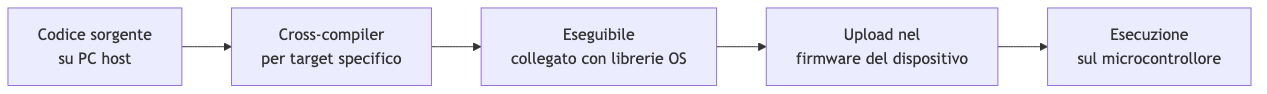
\includegraphics[keepaspectratio]{images/mermaid-lezione-23-embedded-programming-e-arduino-01.png}}
\caption{Pipeline di sviluppo per sistemi embedded: dal codice sorgente
all'eseguibile nel firmware.}
\end{figure}

L'eseguibile finale include il codice del programmatore, le librerie del
sistema operativo e tutta la logica di inizializzazione. La funzione
\texttt{main} è tipicamente fornita dall'OS e si occupa di invocare le
funzioni di inizializzazione scritte dal programmatore, dopodiché attiva
i task che implementano le funzionalità del dispositivo.

\begin{center}\rule{0.5\linewidth}{0.5pt}\end{center}

\section{Organizzazione del Software
Embedded}\label{organizzazione-del-software-embedded}

Il lavoro di un sistema embedded è \textbf{ciclico} per natura, il che
definisce un \textbf{duty cycle}. Il ciclo tipico consiste in:

\begin{enumerate}
\def\labelenumi{\arabic{enumi}.}
\tightlist
\item
  Lettura dai trasduttori (sensori)
\item
  Presa di decisione
\item
  Controllo degli attuatori
\item
  Eventuale comunicazione con altri dispositivi
\end{enumerate}

Questi passi vengono eseguiti in un \textbf{control loop}, una funzione
invocata dal main dopo l'inizializzazione e ripetuta indefinitamente. A
basso livello, il codice interagisce con l'hardware tramite
\textbf{comandi} e \textbf{interrupt}: un comando attiva l'hardware (es.
avvia una lettura da un sensore), mentre un interrupt segnala che il
comando è stato completato.

\begin{callouttip}{Differenza nei sistemi convenzionali vs embedded}

In un OS convenzionale, i comandi sono system call: se c'è da aspettare,
il thread viene sospeso e il kernel gestisce gli interrupt riattivando i
thread sospesi. Questo richiede uno stack per ogni thread. In un sistema
embedded con poca RAM (es. Arduino 1 ha 4 KB), salvare il contesto di
più thread diventa un problema critico.

\end{callouttip}

\begin{center}\rule{0.5\linewidth}{0.5pt}\end{center}

\section{Modelli di Programmazione per
Embedded}\label{modelli-di-programmazione-per-embedded}

Il problema della gestione dell'I/O con memoria limitata ha portato allo
sviluppo di diversi modelli di programmazione. I due esempi principali
sono il \textbf{modello Arduino} (event loop sincrono) e il
\textbf{modello TinyOS} (eventi + task asincroni).

\subsection{Il Modello Arduino}\label{il-modello-arduino}

Arduino adotta un approccio estremamente semplice: il lavoro è definito
in una singola funzione \texttt{loop()}, eseguita ripetutamente da
\textbf{un unico thread}. Non c'è sospensione del thread, non ci sono
context switch. Se un'operazione di I/O richiede tempo, si aspetta
semplicemente che si completi. Se serve un ritardo, si usa
\texttt{delay()} che mette il thread in attesa per il tempo specificato.

\begin{figure}
\centering
\pandocbounded{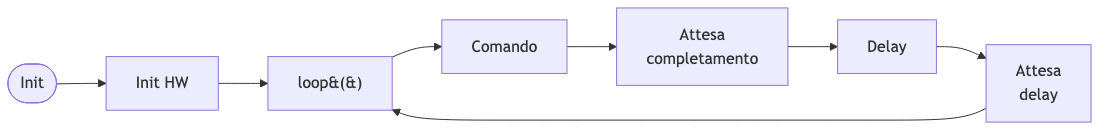
\includegraphics[keepaspectratio]{images/mermaid-lezione-23-embedded-programming-e-arduino-02.png}}
\caption{Modello di esecuzione Arduino: singolo thread, nessuna
sospensione, polling sincrono.}
\end{figure}

\begin{calloutnote}{Pro e contro del modello Arduino}

Il modello è semplice e si adatta bene ad attività di sensing e
controllo. Include librerie per molti attuatori. Tuttavia non è stato
pensato per le comunicazioni asincrone, anche se le versioni recenti
includono librerie (e hardware) per questo scopo. Per le comunicazioni
via linea seriale, Arduino offre anche la gestione asincrona tramite
\textbf{interrupt}.

\end{calloutnote}

\subsection{Il Modello TinyOS}\label{il-modello-tinyos}

{[}{[}TinyOS{]}{]} adotta un approccio diverso, progettato per
massimizzare l'efficienza energetica e gestire attività indipendenti
senza sprecare memoria per i contesti dei thread. Il modello si basa su
tre elementi:

\begin{calloutdefinition}{Comandi, Eventi e Task in TinyOS}

\begin{itemize}
\tightlist
\item
  \textbf{Comandi}: funzioni per programmare e attivare l'hardware
  (verso il basso nella gerarchia).
\item
  \textbf{Eventi}: astrazioni degli interrupt sotto forma di
  \emph{upcall} --- il programmatore definisce un handler per ogni
  evento. Gli eventi possono pre-emptare i task.
\item
  \textbf{Task}: unità di elaborazione non-preemptive eseguite
  sequenzialmente. Un task non aspetta mai (salva memoria). Se un event
  handler richiede elaborazione complessa, posta un task.
\end{itemize}

\end{calloutdefinition}

\begin{figure}
\centering
\pandocbounded{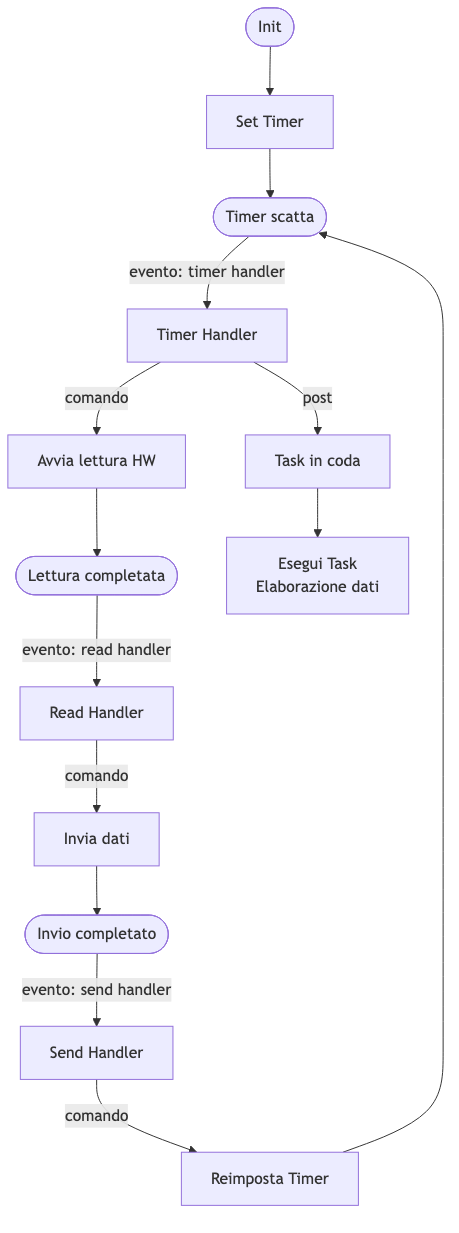
\includegraphics[keepaspectratio]{images/mermaid-lezione-23-embedded-programming-e-arduino-03.png}}
\caption{Flusso di esecuzione TinyOS: eventi gestiti immediatamente,
elaborazione delegata ai task.}
\end{figure}

\subsection{Il Modello degli Eventi: Tre
Livelli}\label{il-modello-degli-eventi-tre-livelli}

Il modello a eventi in TinyOS (e per analogia in Arduino con gli
interrupt) si struttura in tre livelli:

\begin{figure}
\centering
\pandocbounded{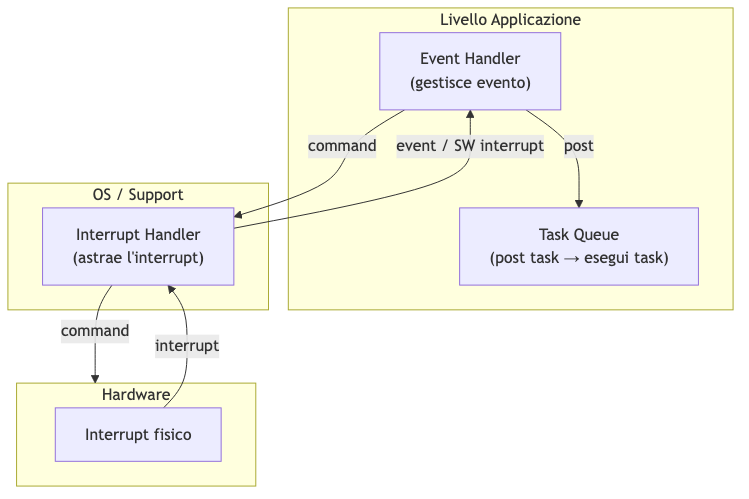
\includegraphics[keepaspectratio]{images/mermaid-lezione-23-embedded-programming-e-arduino-04.png}}
\caption{Modello a tre livelli: hardware genera interrupt, OS li astrae
in eventi, l'applicazione li gestisce con handler e task.}
\end{figure}

\begin{calloutwarning}{Rischio di interferenza}

Un event handler opera in contesto di interrupt, quindi ha accesso
diretto alle strutture dati dell'OS/support. Bisogna fare molta
attenzione a non corrompere queste strutture. Per questo gli event
handler devono essere \textbf{il più corti possibile}: aggiornano
strutture dati, inviano comandi all'HW, e se serve altro lavoro postano
un task.

\end{calloutwarning}

\begin{center}\rule{0.5\linewidth}{0.5pt}\end{center}

\section{Arduino: Case Study}\label{arduino-case-study}

\subsection{La Scheda Arduino Uno}\label{la-scheda-arduino-uno}

Arduino è una piattaforma open-source di prototipazione elettronica
basata su hardware flessibile e software facile da usare. Il concetto
``Arduino'' comprende il \textbf{dispositivo} (la scheda),
l'\textbf{IDE} di sviluppo e il \textbf{forum} della community.

La versione più diffusa è \textbf{Arduino Uno}, basata sul
microcontrollore AVR \textbf{ATmega328}:

\begin{figure}
\centering
\pandocbounded{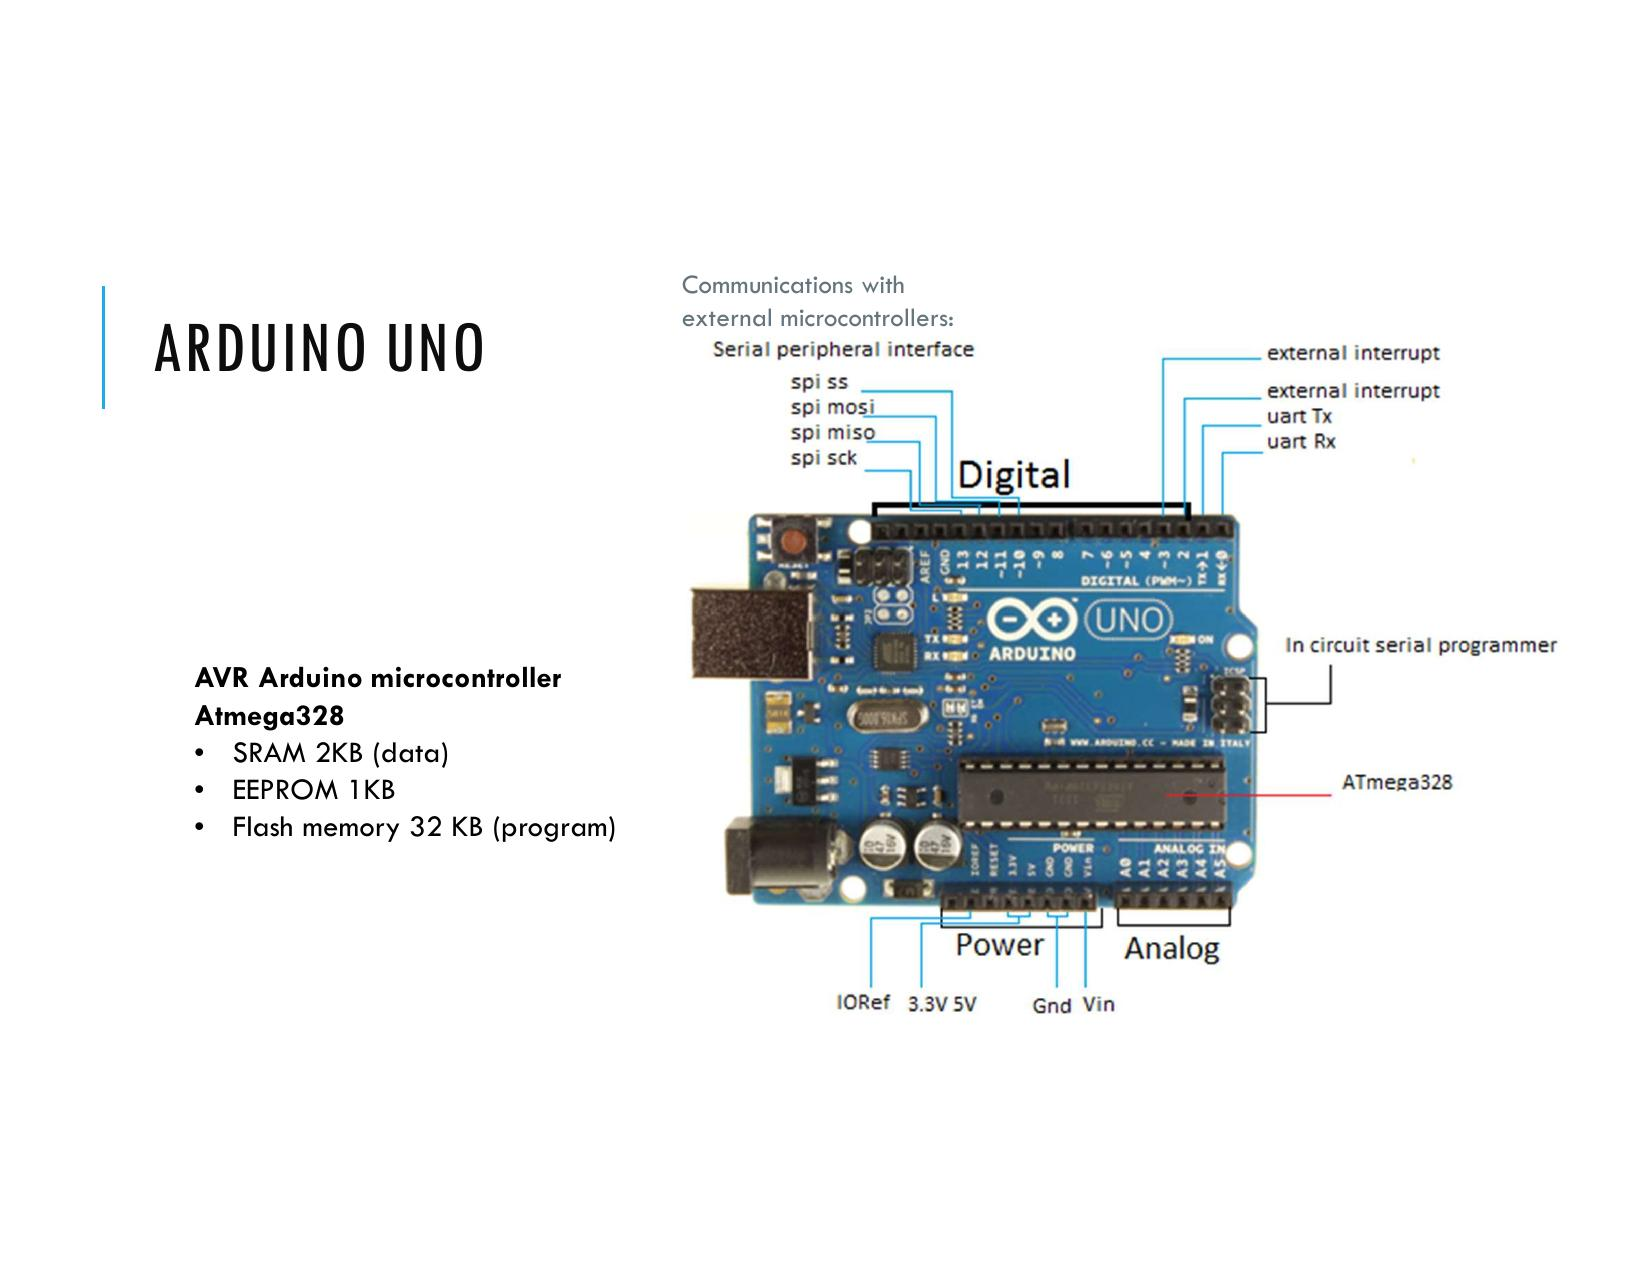
\includegraphics[keepaspectratio]{images/lezione-23-embedded-programming-e-arduino-img-01.jpg}}
\caption{Arduino Uno: microcontrollore ATmega328 con connettori
digitali, analogici, SPI, UART e interrupt esterni.}
\end{figure}

{\def\LTcaptype{none} % do not increment counter
\begin{longtable}[]{@{}lll@{}}
\toprule\noalign{}
Memoria & Dimensione & Uso \\
\midrule\noalign{}
\endhead
\bottomrule\noalign{}
\endlastfoot
SRAM & 2 KB & Dati (variabili, stack) \\
EEPROM & 1 KB & Dati non volatili \\
Flash & 32 KB & Programma (firmware) \\
\end{longtable}
}

La scheda espone pin \textbf{digitali} (con supporto PWM), pin
\textbf{analogici} (input), pin per la comunicazione \textbf{SPI}
(\emph{Serial Peripheral Interface}), linee \textbf{UART} (TX/RX) e due
pin dedicati agli \textbf{interrupt esterni} (pin 2 e 3, corrispondenti
a INT0 e INT1).

\subsection{L'IDE Arduino e la
Cross-Compilazione}\label{lide-arduino-e-la-cross-compilazione}

L'ambiente di sviluppo Arduino (scaricabile da arduino.cc) è scritto in
Java e si basa su Processing, avr-gcc e altri tool open-source. Per
configurare un nuovo progetto è necessario:

\begin{enumerate}
\def\labelenumi{\arabic{enumi}.}
\tightlist
\item
  Scaricare e installare il software Arduino
\item
  Collegare il dispositivo via USB
\item
  Selezionare il tipo di scheda (\texttt{Tools\ →\ Board})
\item
  Selezionare la porta di connessione (\texttt{Tools\ →\ Port})
\item
  Scrivere il codice (\emph{sketch}) e caricarlo
\end{enumerate}

\subsection{Linguaggio e Struttura degli
Sketch}\label{linguaggio-e-struttura-degli-sketch}

\begin{calloutdefinition}{Terminologia Arduino}

\begin{itemize}
\tightlist
\item
  \textbf{Sketch}: un programma scritto per girare su una scheda Arduino
\item
  \textbf{Pin}: un ingresso o uscita connesso a qualcosa (es. output
  verso un LED, input da un potenziometro)
\item
  \textbf{Digital}: valore binario HIGH o LOW (on/off)
\item
  \textbf{Analog}: valore in un range, tipicamente 0--1023 (es.
  luminosità LED, velocità motore)
\end{itemize}

\end{calloutdefinition}

Il linguaggio Arduino è derivato dal \textbf{C} ed è strutturato in tre
parti principali:

\begin{Shaded}
\begin{Highlighting}[]
\DataTypeTok{void}\NormalTok{ setup}\OperatorTok{()} \OperatorTok{\{}
  \CommentTok{// Codice di inizializzazione: eseguito UNA sola volta}
  \CommentTok{// all\textquotesingle{}avvio o dopo un reset}
\OperatorTok{\}}

\DataTypeTok{void}\NormalTok{ loop}\OperatorTok{()} \OperatorTok{\{}
  \CommentTok{// Codice principale: eseguito ripetutamente}
  \CommentTok{// per tutta la durata del funzionamento}
\OperatorTok{\}}
\end{Highlighting}
\end{Shaded}

La funzione \texttt{setup()} viene invocata una volta sola all'avvio e
serve per configurare i pin (input/output), inizializzare la linea
seriale, ecc. La funzione \texttt{loop()} implementa il control loop
discusso in precedenza ed è il cuore dell'applicazione.

\subsection{Funzioni Principali della Libreria
Arduino}\label{funzioni-principali-della-libreria-arduino}

{\def\LTcaptype{none} % do not increment counter
\begin{longtable}[]{@{}
  >{\raggedright\arraybackslash}p{(\linewidth - 2\tabcolsep) * \real{0.5000}}
  >{\raggedright\arraybackslash}p{(\linewidth - 2\tabcolsep) * \real{0.5000}}@{}}
\toprule\noalign{}
\begin{minipage}[b]{\linewidth}\raggedright
Categoria
\end{minipage} & \begin{minipage}[b]{\linewidth}\raggedright
Funzioni
\end{minipage} \\
\midrule\noalign{}
\endhead
\bottomrule\noalign{}
\endlastfoot
I/O Digitale & \texttt{pinMode()}, \texttt{digitalRead()},
\texttt{digitalWrite()} \\
I/O Analogico & \texttt{analogReference()}, \texttt{analogRead()},
\texttt{analogWrite()} \\
I/O Avanzato & \texttt{tone()}, \texttt{shiftOut()}, \texttt{shiftIn()},
\texttt{pulseIn()} \\
Tempo & \texttt{millis()}, \texttt{micros()}, \texttt{delay()},
\texttt{delayMicroseconds()} \\
Matematica & \texttt{min()}, \texttt{max()}, \texttt{abs()},
\texttt{sin()}, \texttt{cos()}, \texttt{random()} \\
Bit/Byte & \texttt{lowByte()}, \texttt{highByte()}, \texttt{bitRead()},
\texttt{bitWrite()} \\
Interrupt & \texttt{attachInterrupt()}, \texttt{detachInterrupt()},
\texttt{interrupts()}, \texttt{noInterrupts()} \\
Comunicazione & \texttt{Serial}, \texttt{Stream} \\
\end{longtable}
}

\subsection{Esempio: Lettura Analogica e
Digitale}\label{esempio-lettura-analogica-e-digitale}

Il codice seguente legge un segnore analogico dal pin A0 e lo converte
in tensione; controlla il pin digitale 2 (button); se il button è
premuto, accende il LED sul pin 13 e stampa la tensione sulla seriale.

\begin{Shaded}
\begin{Highlighting}[]
\AttributeTok{const} \DataTypeTok{int}\NormalTok{ buttonPin }\OperatorTok{=} \DecValTok{2}\OperatorTok{;}   \CommentTok{// pin del pulsante}
\AttributeTok{const} \DataTypeTok{int}\NormalTok{ ledPin }\OperatorTok{=} \DecValTok{13}\OperatorTok{;}     \CommentTok{// pin del LED}
\DataTypeTok{int}\NormalTok{ buttonState }\OperatorTok{=} \DecValTok{0}\OperatorTok{;}       \CommentTok{// stato del pulsante}

\DataTypeTok{void}\NormalTok{ setup}\OperatorTok{()} \OperatorTok{\{}
\NormalTok{  Serial}\OperatorTok{.}\NormalTok{begin}\OperatorTok{(}\DecValTok{9600}\OperatorTok{);}           \CommentTok{// inizializza seriale a 9600 bps}
\NormalTok{  pinMode}\OperatorTok{(}\NormalTok{ledPin}\OperatorTok{,}\NormalTok{ OUTPUT}\OperatorTok{);}      \CommentTok{// LED come output}
\NormalTok{  pinMode}\OperatorTok{(}\NormalTok{buttonPin}\OperatorTok{,}\NormalTok{ INPUT}\OperatorTok{);}    \CommentTok{// pulsante come input}
\OperatorTok{\}}

\DataTypeTok{void}\NormalTok{ loop}\OperatorTok{()} \OperatorTok{\{}
\NormalTok{  buttonState }\OperatorTok{=}\NormalTok{ digitalRead}\OperatorTok{(}\NormalTok{buttonPin}\OperatorTok{);}

  \ControlFlowTok{if} \OperatorTok{(}\NormalTok{buttonState }\OperatorTok{==}\NormalTok{ HIGH}\OperatorTok{)} \OperatorTok{\{}        \CommentTok{// se il pulsante è premuto}
\NormalTok{    digitalWrite}\OperatorTok{(}\NormalTok{ledPin}\OperatorTok{,}\NormalTok{ HIGH}\OperatorTok{);}      \CommentTok{// accende il LED}
    \DataTypeTok{int}\NormalTok{ sensorValue }\OperatorTok{=}\NormalTok{ analogRead}\OperatorTok{(}\NormalTok{A0}\OperatorTok{);}            \CommentTok{// legge [0, 1023]}
    \DataTypeTok{float}\NormalTok{ voltage }\OperatorTok{=}\NormalTok{ sensorValue }\OperatorTok{*} \OperatorTok{(}\FloatTok{5.0} \OperatorTok{/} \FloatTok{1023.0}\OperatorTok{);} \CommentTok{// converte in [0, 5V]}
\NormalTok{    Serial}\OperatorTok{.}\NormalTok{println}\OperatorTok{(}\NormalTok{voltage}\OperatorTok{);}
  \OperatorTok{\}} \ControlFlowTok{else} \OperatorTok{\{}
\NormalTok{    digitalWrite}\OperatorTok{(}\NormalTok{ledPin}\OperatorTok{,}\NormalTok{ LOW}\OperatorTok{);}       \CommentTok{// spegne il LED}
  \OperatorTok{\}}
\OperatorTok{\}}
\end{Highlighting}
\end{Shaded}

\begin{callouttip}{Calcolo del Duty Cycle}

Dato il seguente loop:

\begin{Shaded}
\begin{Highlighting}[]
\DataTypeTok{void}\NormalTok{ loop}\OperatorTok{()} \OperatorTok{\{}
  \DataTypeTok{int}\NormalTok{ sensorValue }\OperatorTok{=}\NormalTok{ analogRead}\OperatorTok{(}\NormalTok{A0}\OperatorTok{);}  \CommentTok{// 2 ms}
\NormalTok{  Serial}\OperatorTok{.}\NormalTok{println}\OperatorTok{(}\NormalTok{sensorValue}\OperatorTok{);}       \CommentTok{// 5 ms}
\NormalTok{  delay}\OperatorTok{(}\DecValTok{100}\OperatorTok{);}                        \CommentTok{// 100 ms}
\OperatorTok{\}}
\end{Highlighting}
\end{Shaded}

\begin{itemize}
\tightlist
\item
  Tempo attivo = 2 + 5 = \textbf{7 ms}
\item
  Periodo totale = 2 + 5 + 100 = \textbf{107 ms}
\item
  \textbf{Duty cycle = 7/107 ≈ 6.5\%}
\end{itemize}

Il sistema è attivo solo per circa il 7\% del tempo --- spazio per
ottimizzare il consumo energetico.

\end{callouttip}

\begin{center}\rule{0.5\linewidth}{0.5pt}\end{center}

\section{Interrupt in Arduino}\label{interrupt-in-arduino}

Sebbene il modello base di Arduino sia la lettura sincrona dei sensori
nel loop, Arduino offre anche un'interfaccia per gli \textbf{interrupt},
che abilita l'accesso asincrono a sensori e attuatori.

\subsection{Tipi di Interrupt}\label{tipi-di-interrupt}

Arduino prevede tre tipi di interrupt:

\begin{itemize}
\tightlist
\item
  \textbf{External}: segnale esterno connesso a un pin
\item
  \textbf{Timer}: interno ad Arduino, gestito dal runtime
\item
  \textbf{Device}: segnale interno proveniente da un dispositivo (ADC,
  seriale, ecc.)
\end{itemize}

Gli interrupt interni (Timer e Device) sono gestiti direttamente dal
runtime di Arduino. Il programmatore si occupa principalmente degli
\textbf{interrupt esterni}.

\subsection{\texorpdfstring{Interrupt Esterni:
\texttt{attachInterrupt()}}{Interrupt Esterni: attachInterrupt()}}\label{interrupt-esterni-attachinterrupt}

\begin{Shaded}
\begin{Highlighting}[]
\NormalTok{attachInterrupt}\OperatorTok{(}\NormalTok{interrupt}\ErrorTok{\#, func{-}name, mode);}
\end{Highlighting}
\end{Shaded}

Arduino Uno dispone di \textbf{soli due pin per interrupt esterni}: INT0
(pin 2) e INT1 (pin 3). Le modalità di trigger disponibili sono:

{\def\LTcaptype{none} % do not increment counter
\begin{longtable}[]{@{}ll@{}}
\toprule\noalign{}
Modalità & Descrizione \\
\midrule\noalign{}
\endhead
\bottomrule\noalign{}
\endlastfoot
\texttt{RISING} & L'interrupt scatta quando il pin passa da LOW a
HIGH \\
\texttt{FALLING} & L'interrupt scatta quando il pin passa da HIGH a
LOW \\
\texttt{CHANGE} & L'interrupt scatta ad ogni cambio di stato \\
\texttt{LOW} & L'interrupt scatta continuamente finché il pin è LOW \\
\texttt{HIGH} & L'interrupt scatta continuamente finché il pin è HIGH \\
\end{longtable}
}

\begin{calloutwarning}{LOW e HIGH non richiedono un cambio di stato}

Con le modalità \texttt{LOW} e \texttt{HIGH}, l'interrupt si attiva
\textbf{ripetutamente} finché il pin rimane in quello stato, anche senza
variazioni. Usarle con cautela.

\end{calloutwarning}

\subsection{Esempio con Interrupt
Esterno}\label{esempio-con-interrupt-esterno}

Il circuito collega un pulsante al pin digitale 2 (con resistore da 10
KΩ) e un LED verde al pin digitale 7 (con resistore da 220 Ω):

\begin{figure}
\centering
\pandocbounded{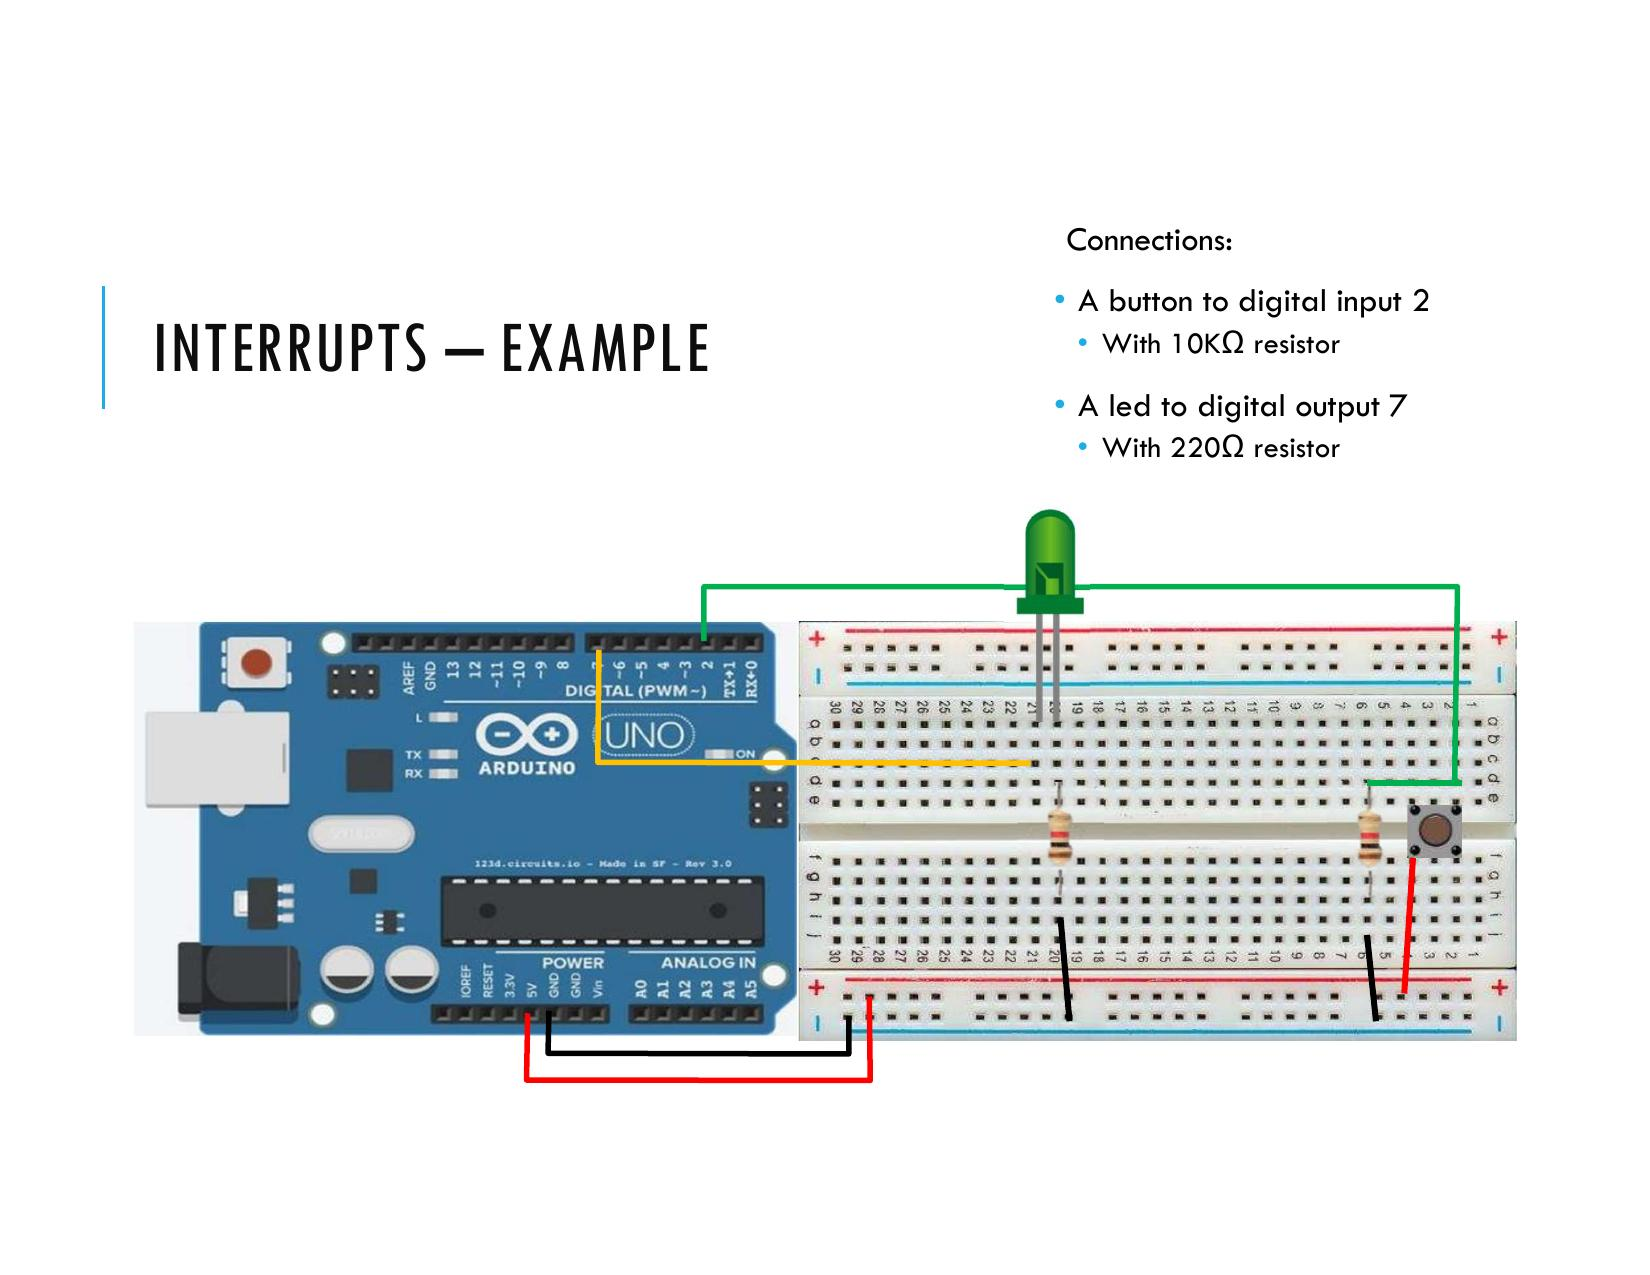
\includegraphics[keepaspectratio]{images/lezione-23-embedded-programming-e-arduino-img-02.jpg}}
\caption{Circuito di esempio: pulsante sul pin 2 (INT0) con resistore
pull-down 10KΩ, LED verde sul pin 7 con resistore 220Ω.}
\end{figure}

\begin{Shaded}
\begin{Highlighting}[]
\AttributeTok{volatile} \DataTypeTok{int}\NormalTok{ greenLed }\OperatorTok{=} \DecValTok{7}\OperatorTok{;}
\AttributeTok{volatile} \DataTypeTok{int}\NormalTok{ count }\OperatorTok{=} \DecValTok{0}\OperatorTok{;}

\DataTypeTok{void}\NormalTok{ setup}\OperatorTok{()} \OperatorTok{\{}
\NormalTok{  Serial}\OperatorTok{.}\NormalTok{begin}\OperatorTok{(}\DecValTok{9600}\OperatorTok{);}
\NormalTok{  pinMode}\OperatorTok{(}\NormalTok{greenLed}\OperatorTok{,}\NormalTok{ OUTPUT}\OperatorTok{);}
\NormalTok{  digitalWrite}\OperatorTok{(}\NormalTok{greenLed}\OperatorTok{,}\NormalTok{ LOW}\OperatorTok{);}
\NormalTok{  attachInterrupt}\OperatorTok{(}\DecValTok{0}\OperatorTok{,}\NormalTok{ interruptSwitchGreen}\OperatorTok{,}\NormalTok{ RISING}\OperatorTok{);} \CommentTok{// 0 = pin 2}
\OperatorTok{\}}

\DataTypeTok{void}\NormalTok{ loop}\OperatorTok{()} \OperatorTok{\{}
\NormalTok{  count}\OperatorTok{++;}
\NormalTok{  delay}\OperatorTok{(}\DecValTok{1000}\OperatorTok{);}
  \CommentTok{// Gli interrupt vengono ricevuti anche dentro delay!}
\NormalTok{  Serial}\OperatorTok{.}\NormalTok{print}\OperatorTok{(}\StringTok{"waiting:"}\OperatorTok{);}
\NormalTok{  Serial}\OperatorTok{.}\NormalTok{println}\OperatorTok{(}\NormalTok{count}\OperatorTok{);}
  \ControlFlowTok{if} \OperatorTok{(}\NormalTok{count }\OperatorTok{==} \DecValTok{10}\OperatorTok{)} \OperatorTok{\{}
\NormalTok{    count }\OperatorTok{=} \DecValTok{0}\OperatorTok{;}
\NormalTok{    digitalWrite}\OperatorTok{(}\NormalTok{greenLed}\OperatorTok{,}\NormalTok{ LOW}\OperatorTok{);}
\NormalTok{    Serial}\OperatorTok{.}\NormalTok{println}\OperatorTok{(}\StringTok{"now off"}\OperatorTok{);}
  \OperatorTok{\}}
\OperatorTok{\}}

\DataTypeTok{void}\NormalTok{ interruptSwitchGreen}\OperatorTok{()} \OperatorTok{\{}
\NormalTok{  digitalWrite}\OperatorTok{(}\NormalTok{greenLed}\OperatorTok{,}\NormalTok{ HIGH}\OperatorTok{);}
\NormalTok{  count }\OperatorTok{=} \DecValTok{0}\OperatorTok{;}
\NormalTok{  Serial}\OperatorTok{.}\NormalTok{print}\OperatorTok{(}\StringTok{"now on"}\OperatorTok{);}
\OperatorTok{\}}
\end{Highlighting}
\end{Shaded}

\begin{calloutwarning}{Regole per gli interrupt handler}

\begin{itemize}
\tightlist
\item
  \texttt{delay()} \textbf{non funziona} dentro un interrupt handler
\item
  \texttt{millis()} \textbf{non viene incrementato} dentro un interrupt
  handler\\
\item
  Tutte le variabili condivise tra il loop e l'interrupt handler devono
  essere dichiarate \texttt{volatile} --- questa direttiva al
  compilatore forza la lettura dalla RAM anziché da un registro,
  garantendo la coerenza del valore
\item
  I handler devono essere \textbf{il più brevi possibile}: solo
  aggiornamento di strutture dati e comandi all'HW
\item
  Per disabilitare tutti gli interrupt: \texttt{noInterrupts()} /
  \texttt{interrupts()}
\item
  Per rimuovere un interrupt specifico: \texttt{detachInterrupt()}
\end{itemize}

\end{calloutwarning}

\begin{center}\rule{0.5\linewidth}{0.5pt}\end{center}

\section{Gestione Energetica in
Arduino}\label{gestione-energetica-in-arduino}

I microcontrollori come l'ATmega328P (cuore di Arduino Uno) offrono
diversi \textbf{sleep mode} per ridurre il consumo energetico quando il
sistema è inattivo. Questi possono essere attivati tramite la libreria
\textbf{Low Power} (\texttt{\#include\ "LowPower.h"}).

I meccanismi di wake-up disponibili sono: interrupt interni, interrupt
esterni o reset di sistema.

\subsection{Modalità di Sleep
dell'ATmega328P}\label{modalituxe0-di-sleep-dellatmega328p}

{\def\LTcaptype{none} % do not increment counter
\begin{longtable}[]{@{}
  >{\raggedright\arraybackslash}p{(\linewidth - 4\tabcolsep) * \real{0.3333}}
  >{\raggedright\arraybackslash}p{(\linewidth - 4\tabcolsep) * \real{0.3333}}
  >{\raggedright\arraybackslash}p{(\linewidth - 4\tabcolsep) * \real{0.3333}}@{}}
\toprule\noalign{}
\begin{minipage}[b]{\linewidth}\raggedright
Modalità
\end{minipage} & \begin{minipage}[b]{\linewidth}\raggedright
Cosa rimane attivo
\end{minipage} & \begin{minipage}[b]{\linewidth}\raggedright
Wake-up
\end{minipage} \\
\midrule\noalign{}
\endhead
\bottomrule\noalign{}
\endlastfoot
\textbf{Idle} & SPI, UART, I2C, watchdog, contatori, comparatore
analogico & Qualsiasi interrupt esterno o interno \\
\textbf{ADC Noise Reduction} & ADC, interrupt esterno, UART, I2C,
watchdog, contatori & Reset, interfaccia seriale, interrupt specifici \\
\textbf{Power-Down} & Solo I2C, watchdog, interrupt esterno & Reset,
interfaccia seriale, interrupt specifici (no timer) \\
\textbf{Power-Save} & Come Power-Down + timer/counter se abilitato &
Come Power-Down + timer overflow \\
\textbf{Standby} & Come Power-Down + oscillatore esterno attivo & Come
Power-Down \\
\textbf{Extended Standby} & Come Power-Save + oscillatore esterno attivo
& Come Power-Save \\
\end{longtable}
}

\subsection{Idle Sleep Mode}\label{idle-sleep-mode}

\begin{Shaded}
\begin{Highlighting}[]
\PreprocessorTok{\#include }\ImportTok{"LowPower.h"}

\CommentTok{// Nessun setup richiesto per la libreria}

\DataTypeTok{void}\NormalTok{ loop}\OperatorTok{()} \OperatorTok{\{}
  \CommentTok{// ... lavoro utile ...}
\NormalTok{  LowPower}\OperatorTok{.}\NormalTok{idle}\OperatorTok{(}\NormalTok{SLEEP\_8S}\OperatorTok{,}\NormalTok{ ADC\_OFF}\OperatorTok{,}\NormalTok{ TIMER2\_OFF}\OperatorTok{,}\NormalTok{ TIMER1\_OFF}\OperatorTok{,}
\NormalTok{                TIMER0\_OFF}\OperatorTok{,}\NormalTok{ SPI\_OFF}\OperatorTok{,}\NormalTok{ USART0\_OFF}\OperatorTok{,}\NormalTok{ TWI\_OFF}\OperatorTok{);}
  \CommentTok{// si risveglia automaticamente dopo 8 secondi}
\OperatorTok{\}}
\end{Highlighting}
\end{Shaded}

I periodi di sleep predefiniti disponibili vanno da \texttt{SLEEP\_15MS}
fino a \texttt{SLEEP\_FOREVER}. Non è obbligatorio spegnere tutto: si
può lasciare attivo ciò che serve con \texttt{ADC\_ON},
\texttt{TIMER0\_ON}, ecc.

\subsection{Power-Down Mode}\label{power-down-mode}

La modalità Power-Down è quella a minor consumo: ferma tutti i clock
generati e lascia attivi solo i moduli asincroni.

\begin{Shaded}
\begin{Highlighting}[]
\PreprocessorTok{\#include }\ImportTok{"LowPower.h"}

\DataTypeTok{void}\NormalTok{ loop}\OperatorTok{()} \OperatorTok{\{}
  \CommentTok{// ... lavoro utile ...}
  
  \CommentTok{// Sleep fisso (wake{-}up automatico dopo 8s)}
\NormalTok{  LowPower}\OperatorTok{.}\NormalTok{powerDown}\OperatorTok{(}\NormalTok{SLEEP\_8S}\OperatorTok{,}\NormalTok{ ADC\_OFF}\OperatorTok{,}\NormalTok{ BOD\_OFF}\OperatorTok{);}
  
  \CommentTok{// oppure: sleep fino a interrupt esterno}
\NormalTok{  attachInterrupt}\OperatorTok{(}\DecValTok{0}\OperatorTok{,}\NormalTok{ wakeUp}\OperatorTok{,}\NormalTok{ LOW}\OperatorTok{);}
\NormalTok{  LowPower}\OperatorTok{.}\NormalTok{powerDown}\OperatorTok{(}\NormalTok{SLEEP\_FOREVER}\OperatorTok{,}\NormalTok{ ADC\_OFF}\OperatorTok{,}\NormalTok{ BOD\_OFF}\OperatorTok{);}
\NormalTok{  detachInterrupt}\OperatorTok{(}\DecValTok{0}\OperatorTok{);}
  
  \CommentTok{// ripresa dell\textquotesingle{}esecuzione qui}
\OperatorTok{\}}
\end{Highlighting}
\end{Shaded}

\begin{callouttip}{Quando usare Power-Down vs Power-Save}

Se il timer/counter non è necessario, preferire sempre
\textbf{Power-Down} rispetto a Power-Save: consuma meno e la differenza
ha senso solo se si ha bisogno di wake-up da timer overflow.

\end{callouttip}

\begin{center}\rule{0.5\linewidth}{0.5pt}\end{center}

\newpage

\chapter{Energy Harvesting IoT}\label{energy-harvesting-iot}

Il problema di fondo dei dispositivi IoT è energetico: alimentarli con
una batteria di capacità finita costringe a scegliere tra prestazioni e
durata. Una batteria grande permette lunga vita, ma aumenta dimensioni,
peso e costo; un processore a basso consumo estende la vita ma limita
potenza di calcolo e portata radio. L'\textbf{energy harvesting}
(raccolta di energia) rappresenta un'alternativa strutturale: invece di
ottimizzare il consumo, si raccoglie energia dall'ambiente e si elimina
--- o si riduce drasticamente --- il vincolo della batteria finita.

Se la sorgente è abbondante e disponibile in modo continuo o periodico,
il dispositivo può funzionare «per sempre». Questa prospettiva sposta
l'obiettivo del progettista dalla massimizzazione della vita utile alla
massimizzazione delle prestazioni a parità di disponibilità energetica.

\begin{center}\rule{0.5\linewidth}{0.5pt}\end{center}

\section{Definizioni fondamentali}\label{definizioni-fondamentali}

Tre concetti strutturano l'intero dominio:

\begin{itemize}
\tightlist
\item
  \textbf{Energy source} (sorgente di energia): la fonte primaria (sole,
  vento, vibrazioni, ecc.) da cui l'energia viene estratta.
\item
  \textbf{Harvesting source} (tecnologia di raccolta): il componente
  fisico --- cella solare, turbina, cristallo piezoelettrico, antenna
  --- che converte la sorgente in energia elettrica. La produzione varia
  nel tempo e in funzione delle condizioni ambientali, ed è generalmente
  al di fuori del controllo del progettista.
\item
  \textbf{Load} (carico): l'energia consumata dal dispositivo per le
  proprie attività. Un dispositivo IoT ha molteplici sottosistemi
  (processore, radio, storage, trasduttori/ADC), ciascuno con stati
  propri e consumi differenti; il carico varia quindi nel tempo a
  seconda delle attività in esecuzione.
\end{itemize}

\begin{calloutdefinition}{Harvesting System}

Un sistema che supporta un carico variabile alimentato da una sorgente
di harvesting variabile, anche quando la potenza istantanea della
sorgente non corrisponde al carico.

\end{calloutdefinition}

Il problema chiave è il \textbf{disaccoppiamento} tra produzione e
consumo: la sorgente produce quando l'ambiente lo consente, il
dispositivo consuma quando deve eseguire i propri task.

\subsection{Bilanciamento tra offerta e
domanda}\label{bilanciamento-tra-offerta-e-domanda}

Esistono due approcci principali per adeguare produzione e consumo:

\begin{enumerate}
\def\labelenumi{\arabic{enumi}.}
\tightlist
\item
  \textbf{Adattare il carico} alla disponibilità energetica --- ad
  esempio riducendo la frequenza di campionamento.
\item
  \textbf{Usare un buffer energetico} --- una batteria ricaricabile o un
  supercapacitore che accumula l'eccesso e lo cede nei momenti di
  deficit.
\end{enumerate}

In pratica nessuno dei due approcci è sufficiente da solo: il carico non
può essere ridotto arbitrariamente senza compromettere la funzionalità,
e il buffer è fisicamente limitato e non ideale (ha perdite ed
efficienza di carica \(< 1\)).

\begin{center}\rule{0.5\linewidth}{0.5pt}\end{center}

\section{Architetture di harvesting}\label{architetture-di-harvesting}

\subsection{Harvest-Use}\label{harvest-use}

\begin{figure}
\centering
\pandocbounded{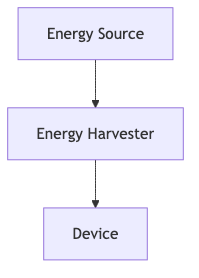
\includegraphics[keepaspectratio]{images/mermaid-lezione-24-energy-harvesting-iot-01.png}}
\caption{Architettura Harvest-Use: la sorgente alimenta direttamente il
dispositivo senza buffer.}
\end{figure}

Nell'architettura \textbf{Harvest-Use} l'energia è raccolta esattamente
quando serve. Non esiste un buffer: la potenza prodotta \(P_s(t)\) viene
consumata istantaneamente. Il dispositivo è operativo solo se:

\[P_s(t) \geq P_c(t)\]

Questo comporta due forme di spreco: - Quando \(P_s(t) < P_c(t)\): il
dispositivo si spegne per mancanza di energia. - Quando
\(P_s(t) > P_c(t)\): l'eccesso \(P_s(t) - P_c(t)\) va perduto.

Variazioni brusche della produzione possono causare oscillazioni
accensione/spegnimento. Esempi tipici: mulini ad acqua, tag RFID
passivi.

\subsection{Harvest-Store-Use}\label{harvest-store-use}

\begin{figure}
\centering
\pandocbounded{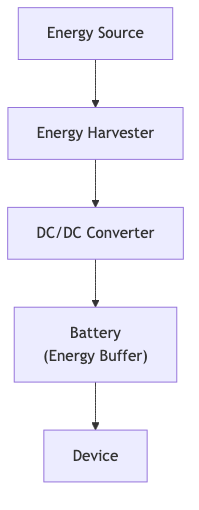
\includegraphics[keepaspectratio]{images/mermaid-lezione-24-energy-harvesting-iot-02.png}}
\caption{Architettura Harvest-Store-Use: l'energia in eccesso viene
accumulata nel buffer e prelevata nei momenti di deficit.}
\end{figure}

Nell'architettura \textbf{Harvest-Store-Use} l'energia raccolta viene
immagazzinata nel buffer ogni volta che è disponibile e prelevata quando
la produzione è insufficiente o i task del dispositivo richiedono più
energia. Il buffer disaccoppia temporalmente produzione e consumo.

\subsubsection{Buffer ideale}\label{buffer-ideale}

Un buffer ideale ha capacità infinita, nessuna perdita ed efficienza di
carica \(\eta = 1\). In queste condizioni il dispositivo è sempre
operativo se, per ogni intervallo \((0, T]\):

\[\int_0^T P_c(t)\,dt \leq \int_0^T P_s(t)\,dt + B_0 \qquad \forall T \in (0, \infty)\]

dove \(B_0\) è la carica iniziale del buffer. La batteria accumula la
potenza prodotta in eccesso \([P_s(t) - P_c(t)]^+\) e cede quella
prodotta in difetto \([P_c(t) - P_s(t)]^+\).

\subsubsection{Buffer non ideale}\label{buffer-non-ideale}

Un buffer reale ha capacità massima \(B_{\mathrm{max}}\), efficienza di
carica \(\eta < 1\) e potenza di leakage \(P_{\mathrm{leak}}(t)\). La
carica \(B_T\) al tempo \(T\) deve soddisfare due equazioni:

\textbf{Conservazione dell'energia (necessaria e sufficiente):}

\[B_T = B_0 + \eta\int_0^T [P_s - P_c]^+\,dt - \int_0^T [P_c - P_s]^+\,dt - \int_0^T P_{\mathrm{leak}}\,dt \geq 0\]

\textbf{Capacità finita (sufficiente, non necessaria):}

\[B_{\mathrm{max}} \geq B_0 + \eta\int_0^T [P_s - P_c]^+\,dt - \int_0^T [P_c - P_s]^+\,dt - \int_0^T P_{\mathrm{leak}}\,dt\]

\begin{calloutnote}{Asimmetria tra le due condizioni}

La condizione di capacità finita è sufficiente ma non necessaria: un
dispositivo può sprecare energia in eccesso (se la sorgente produce più
di quanto il buffer possa contenere) senza violare la conservazione
dell'energia.

\end{calloutnote}

\begin{callouttip}{Esercizio sul buffer non ideale}

Dispositivo con \(\eta = 95\%\), \(B_0 = 400\,\mathrm{mAh}\), leakage
trascurabile.

Intervallo \([0, 4s]\): \(P_s = 80\,\mathrm{mA}\),
\(P_c = 150\,\mathrm{mA}\) --- il consumo supera la produzione. -
Produzione: \(80 \times \frac{4}{3600} = 0.089\,\mathrm{mAh}\); Consumo:
\(150 \times \frac{4}{3600} = 0.167\,\mathrm{mAh}\) -
\(B_4 = 400 + 0.089 - 0.167 = 399.922\,\mathrm{mAh}\)

Intervallo \([4s, 10s]\): \(P_s = 80\,\mathrm{mA}\),
\(P_c = 20\,\mathrm{mA}\) --- la produzione supera il consumo, il buffer
si ricarica. - Produzione:
\(80 \times \frac{6}{3600} = 0.133\,\mathrm{mAh}\); Consumo:
\(20 \times \frac{6}{3600} = 0.033\,\mathrm{mAh}\) -
\(B_{10} = 399.922 + 0.95(0.133 - 0.033) = 400.017\,\mathrm{mAh}\)

\end{callouttip}

\begin{center}\rule{0.5\linewidth}{0.5pt}\end{center}

\section{Fonti di energia e
classificazione}\label{fonti-di-energia-e-classificazione}

Le sorgenti si classificano su due assi: \textbf{controllabilità} e
\textbf{prevedibilità}.

{\def\LTcaptype{none} % do not increment counter
\begin{longtable}[]{@{}
  >{\raggedright\arraybackslash}p{(\linewidth - 4\tabcolsep) * \real{0.3333}}
  >{\raggedright\arraybackslash}p{(\linewidth - 4\tabcolsep) * \real{0.3333}}
  >{\raggedright\arraybackslash}p{(\linewidth - 4\tabcolsep) * \real{0.3333}}@{}}
\toprule\noalign{}
\begin{minipage}[b]{\linewidth}\raggedright
Controllabilità
\end{minipage} & \begin{minipage}[b]{\linewidth}\raggedright
Descrizione
\end{minipage} & \begin{minipage}[b]{\linewidth}\raggedright
Esempi
\end{minipage} \\
\midrule\noalign{}
\endhead
\bottomrule\noalign{}
\endlastfoot
Completamente controllabile & L'energia è disponibile su richiesta &
Torcia shake-to-power, sorgenti RF dedicate \\
Parzialmente controllabile & Influenzabile ma non deterministica & Tag
RFID in ambiente RF non uniforme \\
Non controllabile & Raccolta solo quando disponibile & Sole, vento,
termica ambientale \\
\end{longtable}
}

Le sorgenti non controllabili si classificano ulteriormente in:

{\def\LTcaptype{none} % do not increment counter
\begin{longtable}[]{@{}
  >{\raggedright\arraybackslash}p{(\linewidth - 4\tabcolsep) * \real{0.3333}}
  >{\raggedright\arraybackslash}p{(\linewidth - 4\tabcolsep) * \real{0.3333}}
  >{\raggedright\arraybackslash}p{(\linewidth - 4\tabcolsep) * \real{0.3333}}@{}}
\toprule\noalign{}
\begin{minipage}[b]{\linewidth}\raggedright
Prevedibilità
\end{minipage} & \begin{minipage}[b]{\linewidth}\raggedright
Descrizione
\end{minipage} & \begin{minipage}[b]{\linewidth}\raggedright
Esempi
\end{minipage} \\
\midrule\noalign{}
\endhead
\bottomrule\noalign{}
\endlastfoot
Prevedibile & Esistono modelli affidabili & Sole (ciclo giorno/notte,
stagioni, meteo) \\
Non prevedibile & Nessun modello affidabile & Vibrazioni da terremoti \\
\end{longtable}
}

\begin{callouttip}{Implicazione progettuale}

La prevedibilità è fondamentale per la pianificazione energetica: se la
sorgente è prevedibile si possono pianificare le attività del
dispositivo. Se non lo è, è difficile garantire qualsiasi livello di
prestazione.

\end{callouttip}

\subsection{Tabella comparativa delle sorgenti
principali}\label{tabella-comparativa-delle-sorgenti-principali}

{\def\LTcaptype{none} % do not increment counter
\begin{longtable}[]{@{}
  >{\raggedright\arraybackslash}p{(\linewidth - 10\tabcolsep) * \real{0.1667}}
  >{\raggedright\arraybackslash}p{(\linewidth - 10\tabcolsep) * \real{0.1667}}
  >{\raggedright\arraybackslash}p{(\linewidth - 10\tabcolsep) * \real{0.1667}}
  >{\raggedright\arraybackslash}p{(\linewidth - 10\tabcolsep) * \real{0.1667}}
  >{\raggedright\arraybackslash}p{(\linewidth - 10\tabcolsep) * \real{0.1667}}
  >{\raggedright\arraybackslash}p{(\linewidth - 10\tabcolsep) * \real{0.1667}}@{}}
\toprule\noalign{}
\begin{minipage}[b]{\linewidth}\raggedright
Sorgente
\end{minipage} & \begin{minipage}[b]{\linewidth}\raggedright
Caratteristiche
\end{minipage} & \begin{minipage}[b]{\linewidth}\raggedright
Energia disponibile
\end{minipage} & \begin{minipage}[b]{\linewidth}\raggedright
Tecnologia
\end{minipage} & \begin{minipage}[b]{\linewidth}\raggedright
Efficienza
\end{minipage} & \begin{minipage}[b]{\linewidth}\raggedright
Energia raccolta
\end{minipage} \\
\midrule\noalign{}
\endhead
\bottomrule\noalign{}
\endlastfoot
Solare & Amb., non contr., prevedibile & 100 mW/cm² & Celle solari &
15\% & 15 mW/cm² \\
Vento & Amb., non contr., prevedibile & --- & Anemometro & --- & 1200
mWh/day \\
Vibrazioni (industria) & Controllabile & --- & Piezoelettrico, induzione
& --- & 100 μW/cm² \\
Movimento umano & Controllabile & 19 mW -- 67 W & Piezoelettrico &
7.5--11\% & 2.1 mW -- 5 W \\
Termica (umana) & Non contr., prevedibile & 20 mW/cm² & Termocoppia &
--- & 30 μW/cm² \\
Termica (industriale) & Controllabile & 100 mW/cm² & Termocoppia & --- &
1--10 mW/cm² \\
RF (stazione base) & Controllabile & 0.3 μW/cm² & Antenna & --- & 0.1
μW/cm² \\
Radioattività & --- & 60 mW/cm³ & Decadimento radioattivo & --- & --- \\
\end{longtable}
}

\subsection{Radio Frequency (RF)
harvesting}\label{radio-frequency-rf-harvesting}

Quando un campo RF attraversa una bobina antenna, si genera una tensione
AC. I \textbf{tag RFID passivi} si alimentano esclusivamente con
l'energia RF del reader: il reader trasmette il segnale, il tag
raccoglie l'energia sufficiente per elaborare e rispondere. Non
richiedono alcuna batteria.

\subsection{Piezoelettrico}\label{piezoelettrico}

I materiali piezoelettrici convertono la deformazione meccanica in
differenza di potenziale: - \textbf{PVDF} (PolyVinylidene Fluoride):
film flessibili, adatti a superfici dinamiche. - \textbf{PZT} (Lead
Zirconate Titanate): ceramiche rigide, alta resa.

Applicazioni pratiche: solette per scarpe che alimentano un tag RFID
attivo durante la camminata; pulsanti wireless che trasmettono a 15 m
con una singola pressione, senza batteria.

\subsection{Energia eolica per IoT}\label{energia-eolica-per-iot}

Le micro-turbine per IoT hanno raggio di pochi centimetri, massa
\textasciitilde100 g e operano a velocità del vento basse. La potenza
generata è massima quando la resistenza del carico eguaglia la
resistenza interna del generatore (principio del massimo trasferimento
di potenza). A 10 m/s una micro-turbina tipica eroga \textasciitilde40
mW.

\subsection{Energia solare}\label{energia-solare}

La produzione di un pannello dipende dall'irradianza solare, che varia
con la latitudine, il giorno dell'anno e le condizioni meteorologiche.

\begin{figure}
\centering
\pandocbounded{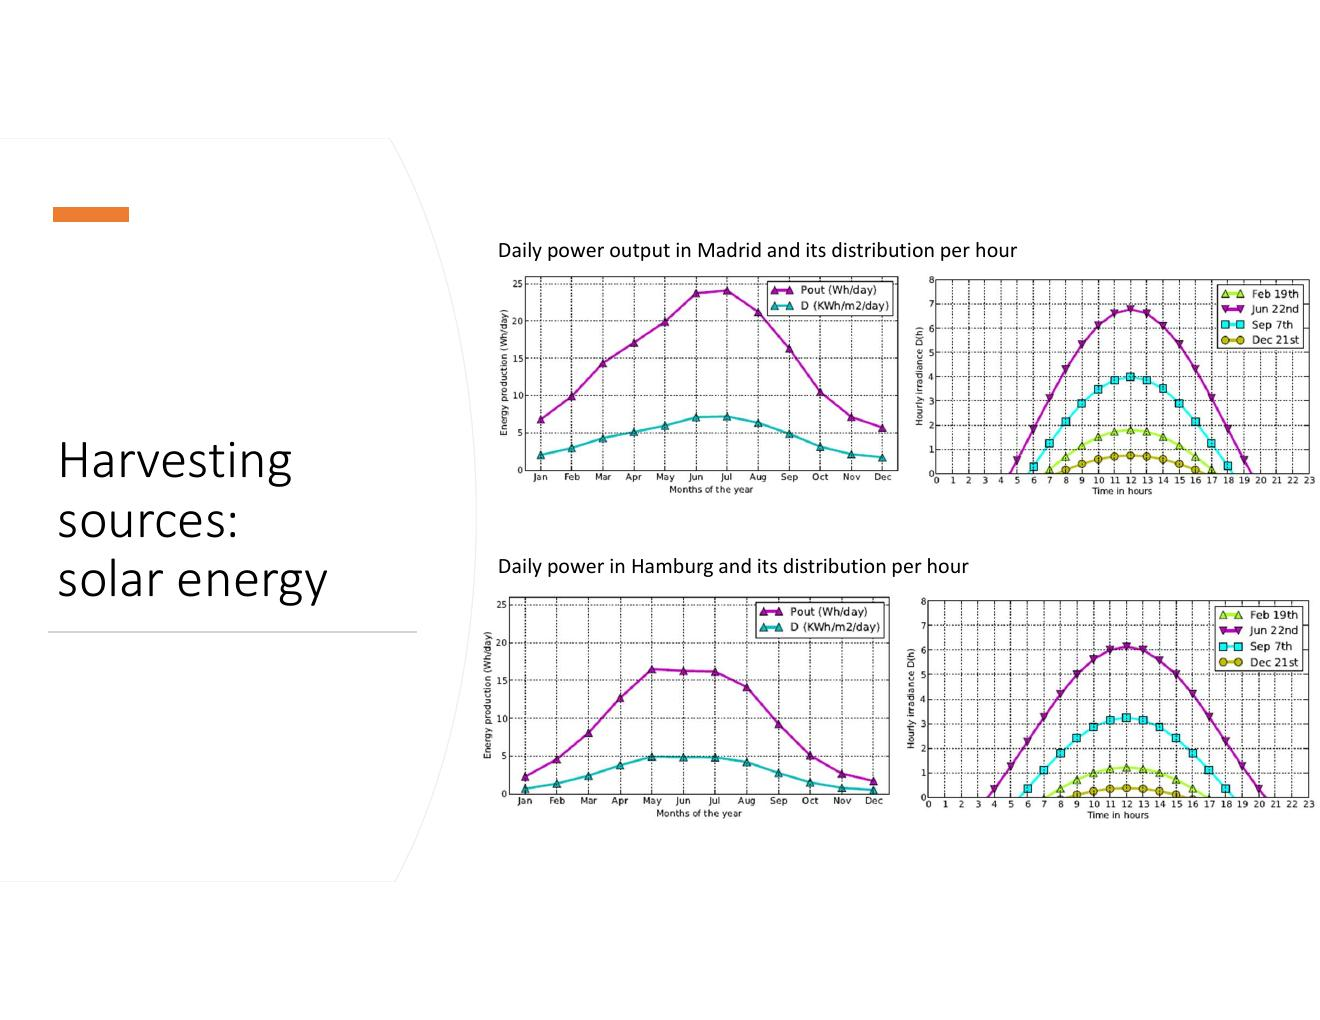
\includegraphics[keepaspectratio]{images/lezione-24-energy-harvesting-iot-img-01.jpg}}
\caption{Produzione solare giornaliera (Wh/day) e irradianza oraria a
Madrid e Amburgo per le quattro stagioni. Madrid raggiunge
\textasciitilde25 Wh/day in estate; Amburgo è più attenuata e
stagionalmente più variabile.}
\end{figure}

La variabilità stagionale è estrema: la \textbf{soluzione classica} è
sovradimensionare il pannello e la batteria per coprire il caso peggiore
(tipicamente dicembre alle latitudini settentrionali).

\begin{figure}
\centering
\pandocbounded{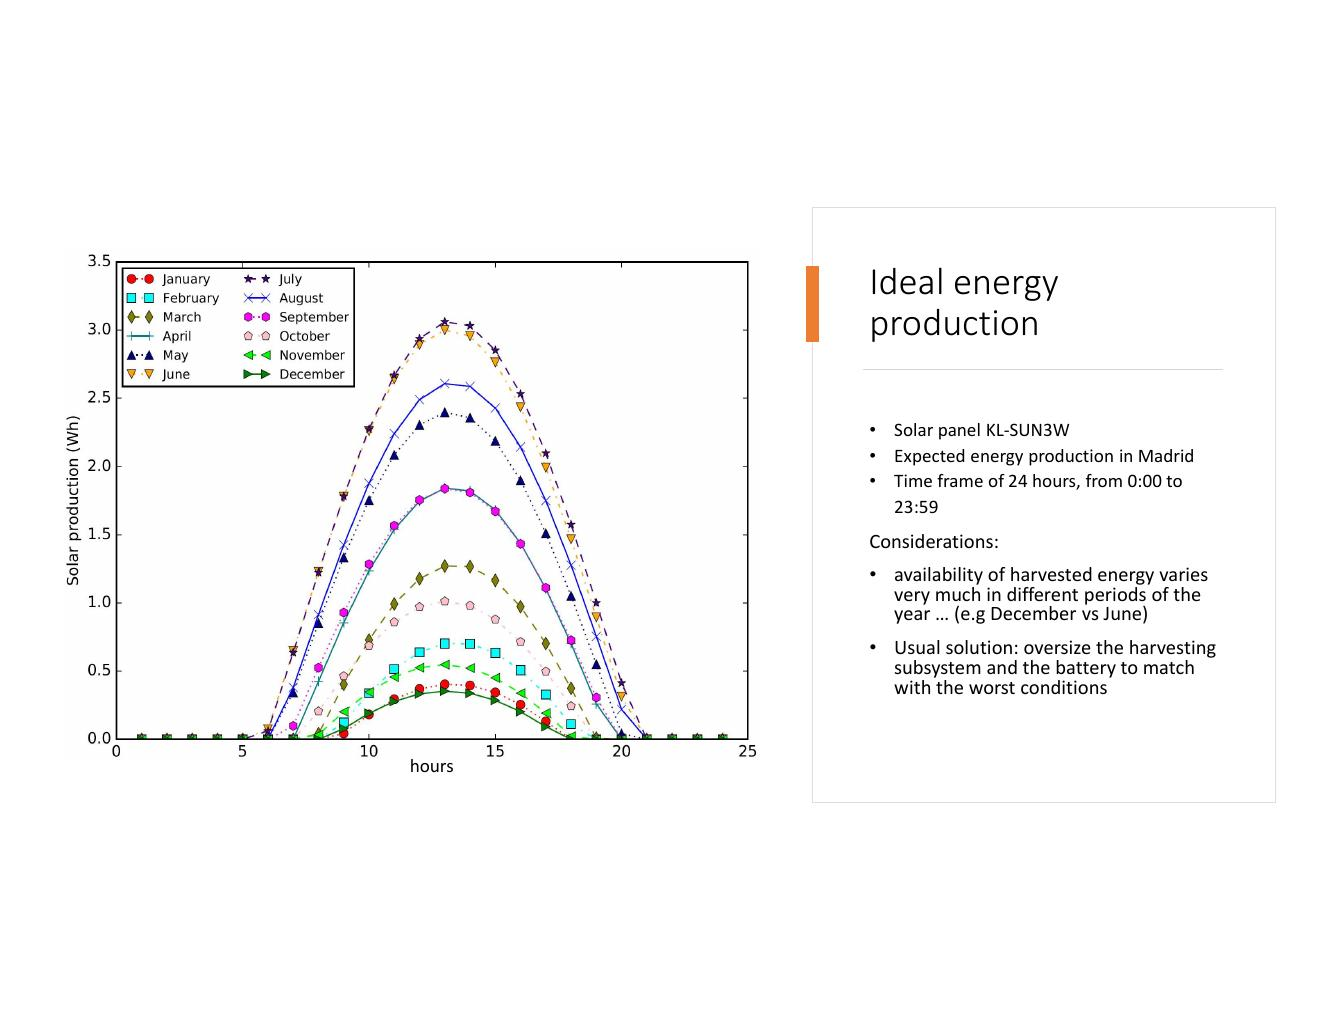
\includegraphics[keepaspectratio]{images/lezione-24-energy-harvesting-iot-img-02.jpg}}
\caption{Produzione oraria stimata del pannello KL-SUN3W a Madrid, mese
per mese (0--24 h). I mesi estivi raggiungono \textasciitilde3 Wh per
slot orario; dicembre e gennaio sono quasi trascurabili.}
\end{figure}

Nella realtà, la produzione effettiva diverge nettamente dalla stima
nelle giornate nuvolose:

\begin{figure}
\centering
\pandocbounded{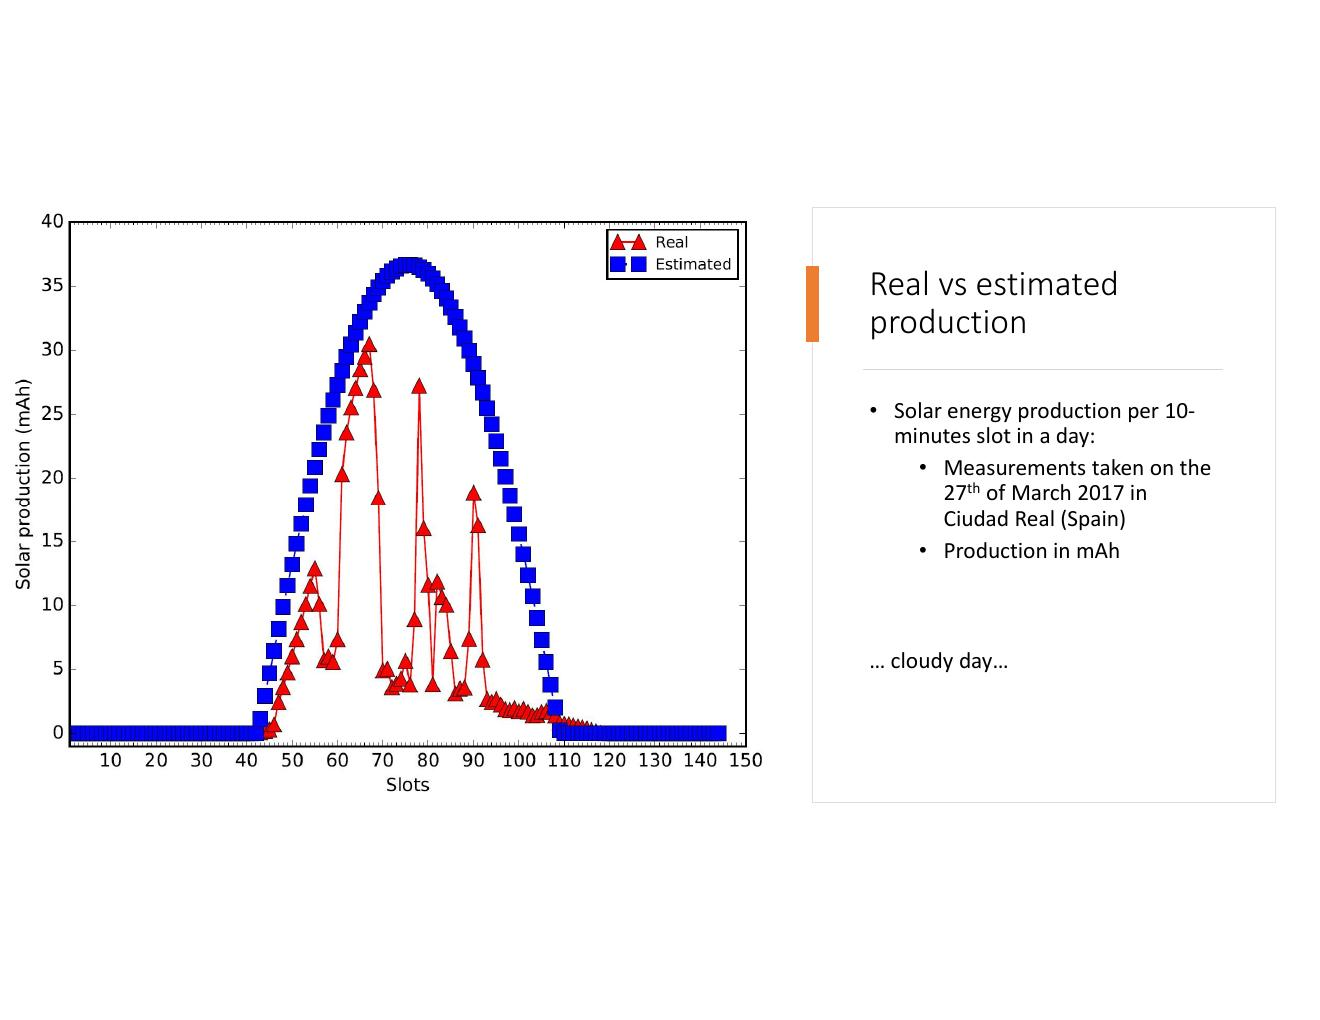
\includegraphics[keepaspectratio]{images/lezione-24-energy-harvesting-iot-img-03.jpg}}
\caption{Produzione reale (triangoli rossi) vs stimata EWMA (quadrati
blu), per slot da 10 minuti. Giornata molto nuvolosa: la produzione
reale è fortemente discontinua e inferiore alla stima.}
\end{figure}

\begin{calloutwarning}{Complementarità sole–vento}

Il sole produce continuamente ma solo di giorno; il vento produce in
modo irregolare ma anche di notte. La combinazione delle due sorgenti
aumenta la copertura temporale.

\end{calloutwarning}

\begin{figure}
\centering
\pandocbounded{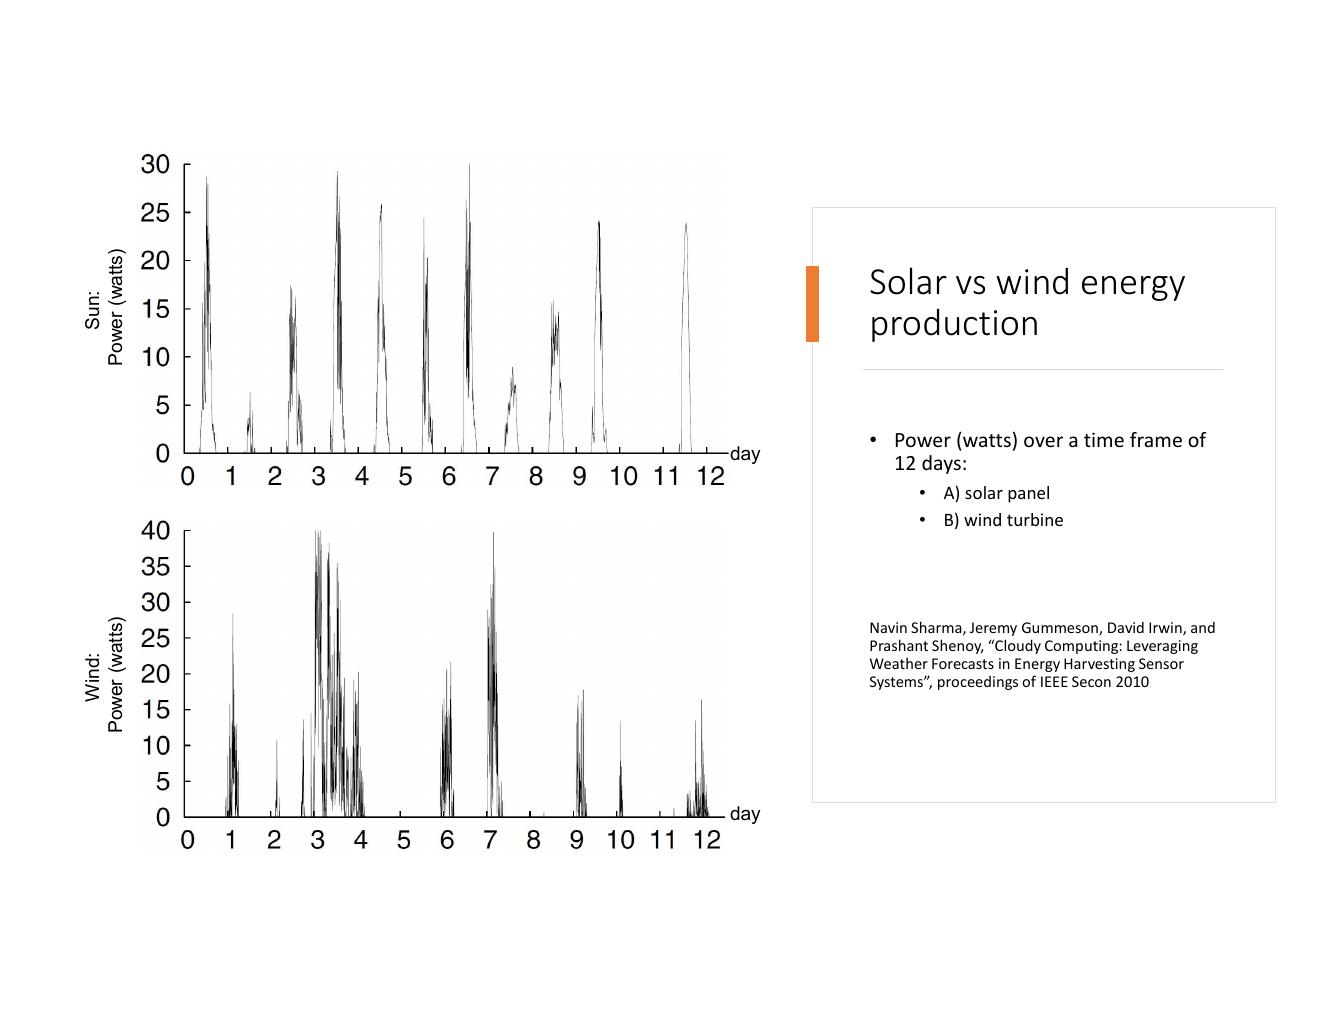
\includegraphics[keepaspectratio]{images/lezione-24-energy-harvesting-iot-img-04.jpg}}
\caption{Potenza (watt) su 12 giorni: sopra, pannello solare (picchi
giornalieri regolari); sotto, turbina eolica (picchi irregolari, anche
notturni). Fonte: Sharma et al., IEEE Secon 2010.}
\end{figure}

\begin{calloutwarning}{Energia harvesting ≠ operatività garantita}

Una notte senza vento con batteria quasi scarica può causare lo
spegnimento del dispositivo. Il progettista deve dimensionare il sistema
per il caso peggiore ragionevole, non per il caso medio.

\end{calloutwarning}

\begin{center}\rule{0.5\linewidth}{0.5pt}\end{center}

\section{Tecnologie di storage}\label{tecnologie-di-storage}

\subsection{Batterie ricaricabili}\label{batterie-ricaricabili}

Le batterie sono celle di immagazzinamento in cui la reazione chimica
interna è reversibile (si può ricaricare invertendo il flusso di
corrente).

{\def\LTcaptype{none} % do not increment counter
\begin{longtable}[]{@{}
  >{\raggedright\arraybackslash}p{(\linewidth - 10\tabcolsep) * \real{0.1667}}
  >{\raggedright\arraybackslash}p{(\linewidth - 10\tabcolsep) * \real{0.1667}}
  >{\raggedright\arraybackslash}p{(\linewidth - 10\tabcolsep) * \real{0.1667}}
  >{\raggedright\arraybackslash}p{(\linewidth - 10\tabcolsep) * \real{0.1667}}
  >{\raggedright\arraybackslash}p{(\linewidth - 10\tabcolsep) * \real{0.1667}}
  >{\raggedright\arraybackslash}p{(\linewidth - 10\tabcolsep) * \real{0.1667}}@{}}
\toprule\noalign{}
\begin{minipage}[b]{\linewidth}\raggedright
Tipo
\end{minipage} & \begin{minipage}[b]{\linewidth}\raggedright
Tensione nom. (V)
\end{minipage} & \begin{minipage}[b]{\linewidth}\raggedright
Densità energetica (Wh/kg)
\end{minipage} & \begin{minipage}[b]{\linewidth}\raggedright
Efficienza (\%)
\end{minipage} & \begin{minipage}[b]{\linewidth}\raggedright
Self-discharge (\%/mese)
\end{minipage} & \begin{minipage}[b]{\linewidth}\raggedright
Cicli
\end{minipage} \\
\midrule\noalign{}
\endhead
\bottomrule\noalign{}
\endlastfoot
SLA (Sealed Lead Acid) & 6 & 26 & 70--92 & 20 & 500--800 \\
NiCd & 1.2 & 42 & 70--90 & 10 & 1500 \\
NiMH & 1.2 & 100 & 66 & 20 & 1000 \\
\textbf{Li-ion} & 3.7 & 165 & \textbf{99.9} & \textless10 & 1200 \\
\end{longtable}
}

La Li-ion è la tecnologia preferita per IoT: altissima efficienza,
bassissimo self-discharge, elevata densità energetica.

\subsection{Supercapacitori}\label{supercapacitori}

{\def\LTcaptype{none} % do not increment counter
\begin{longtable}[]{@{}ll@{}}
\toprule\noalign{}
Parametro & Valore \\
\midrule\noalign{}
\endhead
\bottomrule\noalign{}
\endlastfoot
Densità energetica & 5 Wh/kg \\
Efficienza & 97--98\% \\
Self-discharge & 5.9\%/giorno \\
Cicli di ricarica & \textbf{Infiniti} \\
\end{longtable}
}

I supercapacitori non richiedono circuiti di carica complessi. Sono
ideali quando l'energia è disponibile a intervalli regolari o quando la
sorgente è molto variabile (\emph{jitter}). La modalità \textbf{trickle
charge} mantiene il condensatore pieno caricandolo alla stessa velocità
con cui si scarica.

\begin{center}\rule{0.5\linewidth}{0.5pt}\end{center}

\section{Misurare la carica della
batteria}\label{misurare-la-carica-della-batteria}

Tutte le tecniche di power management richiedono informazioni fresche
sulla carica attuale della batteria e sulla produzione energetica.
Entrambe sono quantità non direttamente osservabili e devono essere
stimate.

\subsection{Relazione tensione--carica}\label{relazione-tensionecarica}

La tensione a circuito aperto di una batteria decresce al diminuire
della carica. Nell'intervallo operativo la relazione è
approssimativamente \textbf{lineare} (la dipendenza dalla tecnologia
specifica è reale: non sempre vale).

\begin{figure}
\centering
\pandocbounded{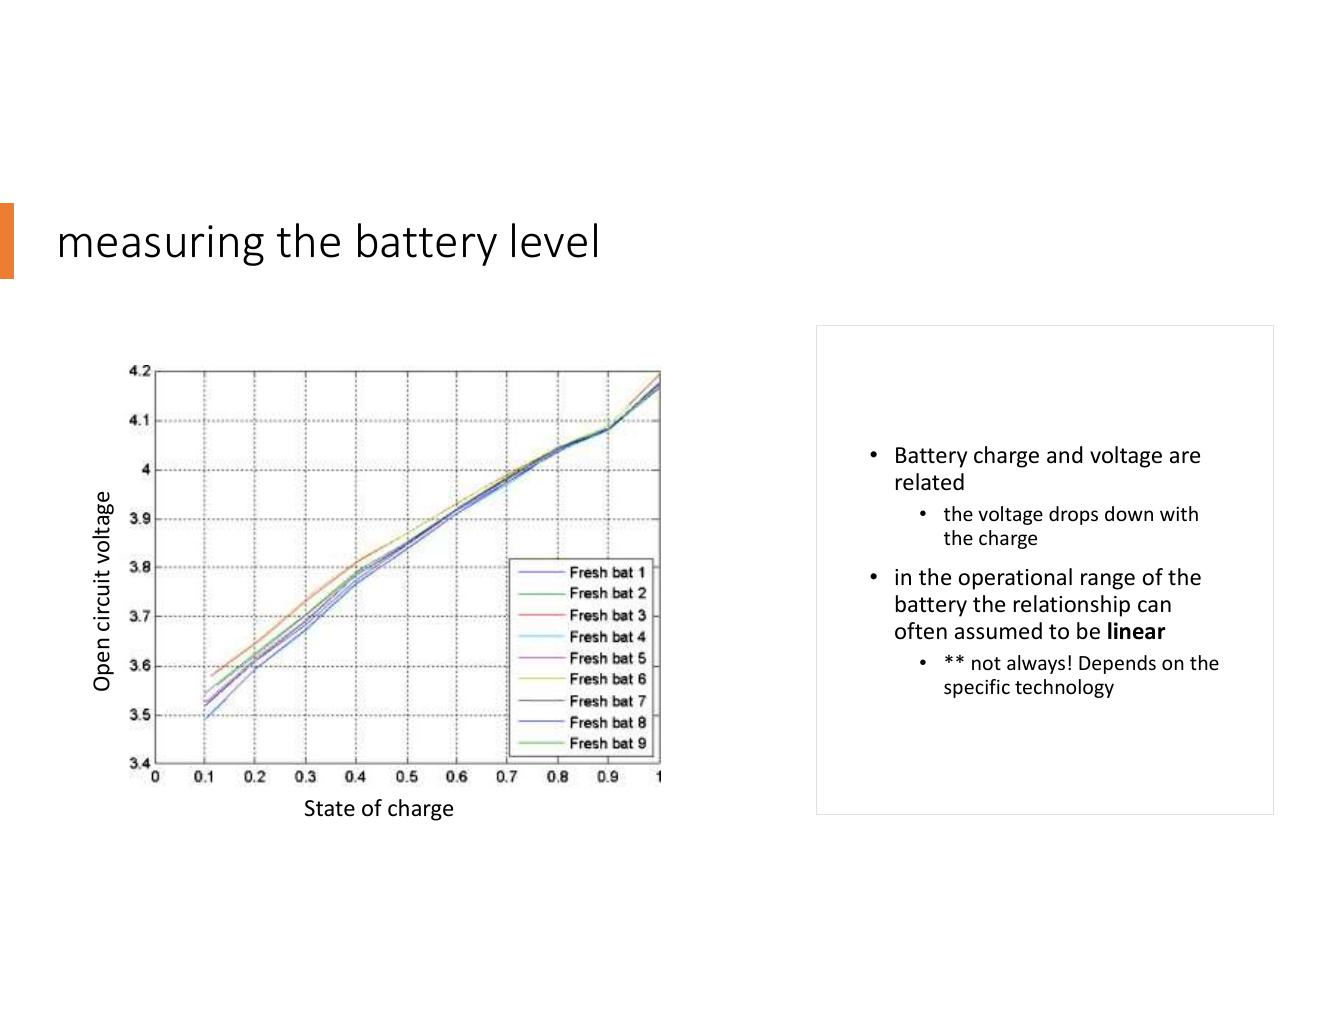
\includegraphics[keepaspectratio]{images/lezione-24-energy-harvesting-iot-img-05.jpg}}
\caption{Tensione a circuito aperto (V) vs stato di carica (0--1) per
nove batterie Li-ion nuove. La relazione è quasi lineare tra 3.4 V e 4.2
V.}
\end{figure}

Sfruttando la linearità, si usa un \textbf{ADC} a \(d\) bit per leggere
la tensione e risalire alla carica. Dati
\(v_{\mathrm{min}}, v_{\mathrm{max}}\) (tensioni corrispondenti a
\(B_{\mathrm{min}}, B_{\mathrm{max}}\)) e la tensione di riferimento
\(v_{\mathrm{ref}}\):

\[x_{\mathrm{max}} = 2^d - 1 \qquad x_{\mathrm{min}} = \mathrm{ROUND}\!\left(\frac{v_{\mathrm{min}}}{v_{\mathrm{ref}}}(2^d - 1)\right)\]

Per una tensione misurata \(v\), il valore ADC è:

\[x = \mathrm{ROUND}\!\left(\frac{v}{v_{\mathrm{ref}}}(2^d - 1)\right)\]

e la carica corrispondente:

\[B = B_{\mathrm{min}} + \frac{B_{\mathrm{max}} - B_{\mathrm{min}}}{x_{\mathrm{max}} - x_{\mathrm{min}}}(x - x_{\mathrm{min}})\]

\begin{callouttip}{Esempi su piattaforme reali (B\_\{\\mathrm\{min\}\} = 300\\,\\mathrm\{mAh\})}

{\def\LTcaptype{none} % do not increment counter
\begin{longtable}[]{@{}
  >{\raggedright\arraybackslash}p{(\linewidth - 18\tabcolsep) * \real{0.1000}}
  >{\raggedright\arraybackslash}p{(\linewidth - 18\tabcolsep) * \real{0.1000}}
  >{\raggedright\arraybackslash}p{(\linewidth - 18\tabcolsep) * \real{0.1000}}
  >{\raggedright\arraybackslash}p{(\linewidth - 18\tabcolsep) * \real{0.1000}}
  >{\raggedright\arraybackslash}p{(\linewidth - 18\tabcolsep) * \real{0.1000}}
  >{\raggedright\arraybackslash}p{(\linewidth - 18\tabcolsep) * \real{0.1000}}
  >{\raggedright\arraybackslash}p{(\linewidth - 18\tabcolsep) * \real{0.1000}}
  >{\raggedright\arraybackslash}p{(\linewidth - 18\tabcolsep) * \real{0.1000}}
  >{\raggedright\arraybackslash}p{(\linewidth - 18\tabcolsep) * \real{0.1000}}
  >{\raggedright\arraybackslash}p{(\linewidth - 18\tabcolsep) * \real{0.1000}}@{}}
\toprule\noalign{}
\begin{minipage}[b]{\linewidth}\raggedright
Piattaforma
\end{minipage} & \begin{minipage}[b]{\linewidth}\raggedright
\(v_{\mathrm{min}}\)
\end{minipage} & \begin{minipage}[b]{\linewidth}\raggedright
\(v_{\mathrm{max}}\)
\end{minipage} & \begin{minipage}[b]{\linewidth}\raggedright
\(v_{\mathrm{ref}}\)
\end{minipage} & \begin{minipage}[b]{\linewidth}\raggedright
ADC (bit)
\end{minipage} & \begin{minipage}[b]{\linewidth}\raggedright
\(x_{\mathrm{min}}\)
\end{minipage} & \begin{minipage}[b]{\linewidth}\raggedright
\(x_{\mathrm{max}}\)
\end{minipage} & \begin{minipage}[b]{\linewidth}\raggedright
Battery (mAh)
\end{minipage} & \begin{minipage}[b]{\linewidth}\raggedright
Campione \(x\)
\end{minipage} & \begin{minipage}[b]{\linewidth}\raggedright
Carica (mAh)
\end{minipage} \\
\midrule\noalign{}
\endhead
\bottomrule\noalign{}
\endlastfoot
Raspberry Pi & 3.5 V & 5 V & 0.00488 V & 10 & 716 & 1023 & 3000 & 1000 &
2798 \\
Arduino & 7 V & 9 V & 0.00879 V & 10 & 795 & 1023 & 3000 & 800 & 359 \\
Tmote & 1.8 V & 3 V & 0.000732 V & 12 & 2457 & 4095 & 3000 & 3277 &
1652 \\
\end{longtable}
}

\end{callouttip}

\begin{callouttip}{Esercizio — Stima della carica da output ADC}

Un dispositivo campiona la tensione della batteria con un ADC a
\textbf{10 bit}. La batteria ha una carica massima di \textbf{2000 mAh}
e una tensione massima (batteria piena) di \textbf{10 V}. Quando la
tensione scende a \textbf{8 V} la carica residua è \textbf{200 mAh} e il
dispositivo non è più alimentabile.

Calcolare la carica della batteria quando l'ADC restituisce:
\textbf{920}, \textbf{830}, \textbf{1023}.

\textbf{Soluzione}

Con \(d = 10\) bit si ha \(2^d - 1 = 1023\) e
\(v_{\mathrm{ref}} = v_{\mathrm{max}} = 10\,\mathrm{V}\).

\[x_{\mathrm{max}} = 1023 \qquad x_{\mathrm{min}} = \mathrm{ROUND}\!\left(\frac{8}{10} \times 1023\right) = \mathrm{ROUND}(818{,}4) = 818\]

La carica si ricava per interpolazione lineare tra
\((x_{\mathrm{min}},\, B_{\mathrm{min}})\) e
\((x_{\mathrm{max}},\, B_{\mathrm{max}})\):

\[B = B_{\mathrm{min}} + \frac{x - x_{\mathrm{min}}}{x_{\mathrm{max}} - x_{\mathrm{min}}} \cdot (B_{\mathrm{max}} - B_{\mathrm{min}})\]

{\def\LTcaptype{none} % do not increment counter
\begin{longtable}[]{@{}
  >{\raggedright\arraybackslash}p{(\linewidth - 4\tabcolsep) * \real{0.3333}}
  >{\raggedright\arraybackslash}p{(\linewidth - 4\tabcolsep) * \real{0.3333}}
  >{\raggedright\arraybackslash}p{(\linewidth - 4\tabcolsep) * \real{0.3333}}@{}}
\toprule\noalign{}
\begin{minipage}[b]{\linewidth}\raggedright
\(x\)
\end{minipage} & \begin{minipage}[b]{\linewidth}\raggedright
Calcolo
\end{minipage} & \begin{minipage}[b]{\linewidth}\raggedright
\(B\) (mAh)
\end{minipage} \\
\midrule\noalign{}
\endhead
\bottomrule\noalign{}
\endlastfoot
920 &
\(200 + \dfrac{920 - 818}{1023 - 818} \times 1800 = 200 + \dfrac{102}{205} \times 1800\)
& \textbf{≈ 1096} \\
830 &
\(200 + \dfrac{830 - 818}{1023 - 818} \times 1800 = 200 + \dfrac{12}{205} \times 1800\)
& \textbf{≈ 305} \\
1023 & \(200 + \dfrac{1023 - 818}{1023 - 818} \times 1800 = 200 + 1800\)
& \textbf{2000} \\
\end{longtable}
}

\end{callouttip}

\subsection{Stima della produzione
energetica}\label{stima-della-produzione-energetica}

Se si conosce il consumo \(p_c(t)\) in un intervallo \([t_1, t_2]\) e si
misura la carica agli estremi, la produzione \(E_s\) si stima come:

\[E_s = \int_{t_1}^{t_2} p_c(t)\,dt + [E(t_2) - E(t_1)]^+\]

Questo presuppone un buffer ideale. I limiti sono: errori di misura
della carica si propagano sulla stima di \(E_s\); intervalli troppo
lunghi non distinguono quando l'energia era disponibile; la stima di
\(p_c(t)\) può non essere precisa. Il metodo alternativo è misurare
direttamente corrente e tensione all'uscita della sorgente con circuiti
elettronici dedicati.

\begin{center}\rule{0.5\linewidth}{0.5pt}\end{center}

\section{Neutralità energetica}\label{neutralituxe0-energetica}

\begin{calloutdefinition}{Dispositivo energy-neutral}

Un dispositivo è \textbf{energy neutral} se riesce a mantenere il
livello di prestazione desiderato indefinitamente, senza mai esaurire la
batteria.

\end{calloutdefinition}

Questo obiettivo è radicalmente diverso dalla classica massimizzazione
della vita utile: qui si mira a prestazioni indefinitamente sostenute,
modulando il carico in funzione della disponibilità energetica.

Nascono due sotto-problemi complementari: 1. \textbf{Energy-Neutral
Operation}: come pianificare le attività in modo che, in qualsiasi
finestra temporale, l'energia consumata non superi quella raccolta? 2.
\textbf{Maximum Performance}: dato l'ambiente di harvesting, qual è il
massimo livello di prestazione sostenibile garantendo la neutralità
energetica?

In sistemi IoT distribuiti il problema si complica: le prestazioni
globali dipendono dalla distribuzione spazio-temporale dell'energia
raccolta da ciascun nodo, e dalle dipendenze tra nodo e server nella
elaborazione dei dati.

\begin{center}\rule{0.5\linewidth}{0.5pt}\end{center}

\section{Approccio di Kansal alla neutralità
energetica}\label{approccio-di-kansal-alla-neutralituxe0-energetica}

Kansal affronta il caso di sorgenti \textbf{non controllabili ma
prevedibili} (tipicamente il sole). L'idea è pianificare dinamicamente
il duty cycle del dispositivo slot per slot, sfruttando previsioni sulla
produzione futura.

L'approccio si concentra su fonti non controllabili ma prevedibili
perché: - Le fonti non prevedibili rendono impossibile qualsiasi
garanzia di prestazione. - Le fonti controllabili rendono il problema
banale (si produce energia quando serve).

\subsection{Condizioni formali}\label{condizioni-formali}

\textbf{Condizione 1 --- Produzione:} l'energia prodotta in \([0, T]\) è
vincolata linearmente:

\pandocbounded{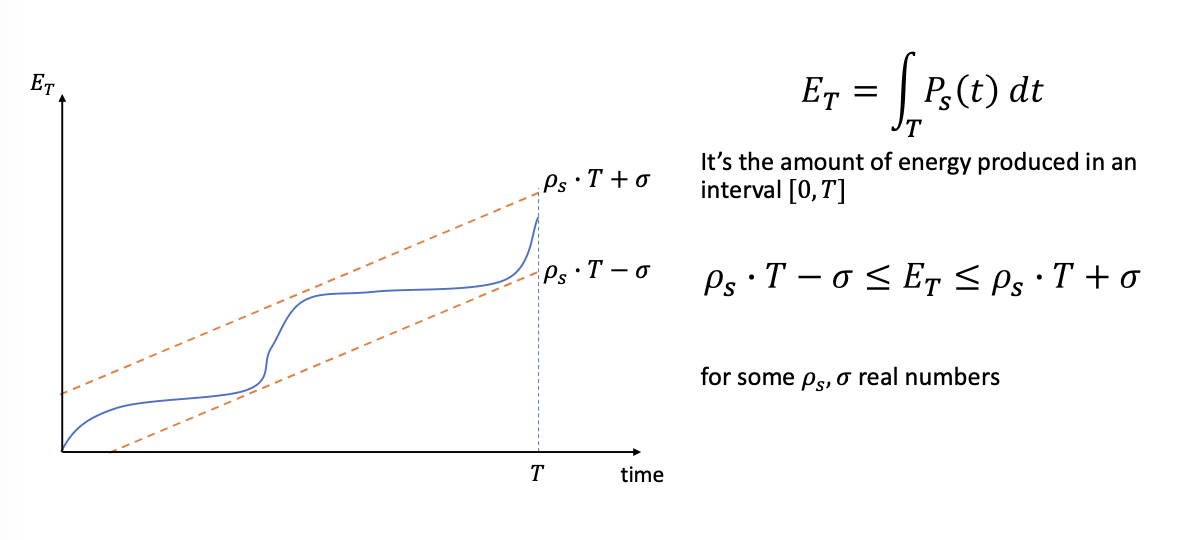
\includegraphics[keepaspectratio]{images/Pasted-image-20260512144552.png}}

\[\rho_s T - \sigma \leq E_s(T) \leq \rho_s T + \sigma\]

\textbf{Condizione 2 --- Carico:} l'energia consumata in \([0, T]\) è
vincolata superiormente:

\pandocbounded{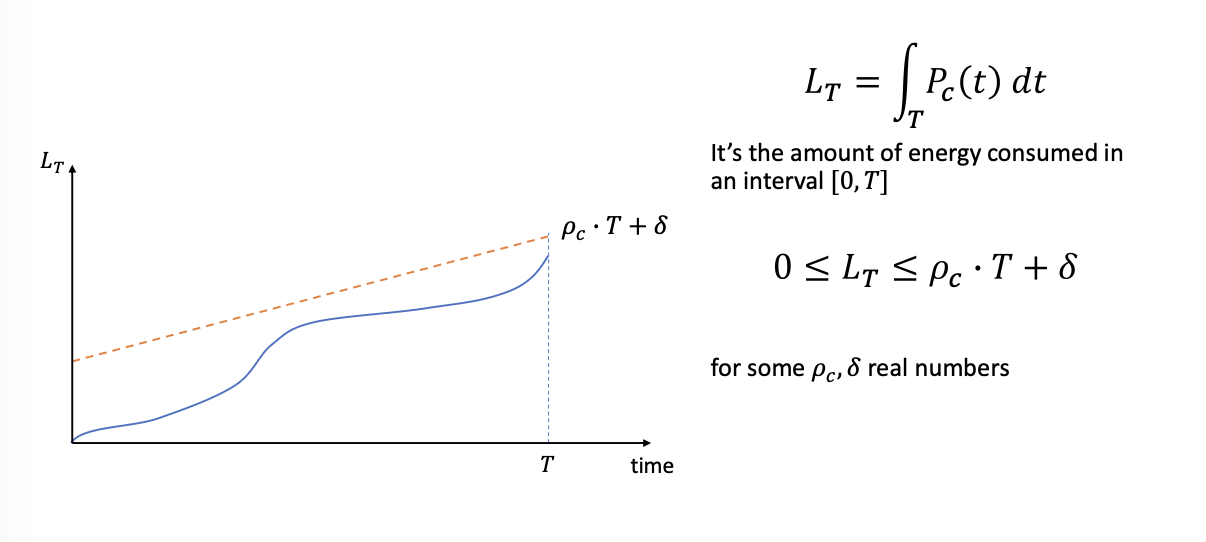
\includegraphics[keepaspectratio]{images/Pasted-image-20260512144607.png}}

\[E_c(T) \leq \rho_c T + \delta\]

\begin{callouttheorem}{Teorema di Kansal}

Se valgono le Condizioni 1 e 2, e il buffer ha efficienza \(\eta\) e
leakage \(\rho_l\), sono condizioni \textbf{sufficienti} per la
neutralità energetica: 1. \(\eta\,\rho_s \geq \rho_c + \rho_l\) --- il
tasso di produzione netta supera consumo più leakage. 2.
\(B_0 \geq \sigma + \delta\) --- la carica iniziale copre le
oscillazioni nel caso peggiore. 3. \(B_{\mathrm{max}} \geq B_0\) --- la
carica iniziale è fisicamente ammissibile.

\end{callouttheorem}

\begin{center}\rule{0.5\linewidth}{0.5pt}\end{center}

\section{Riepilogo}\label{riepilogo}

\begin{figure}
\centering
\pandocbounded{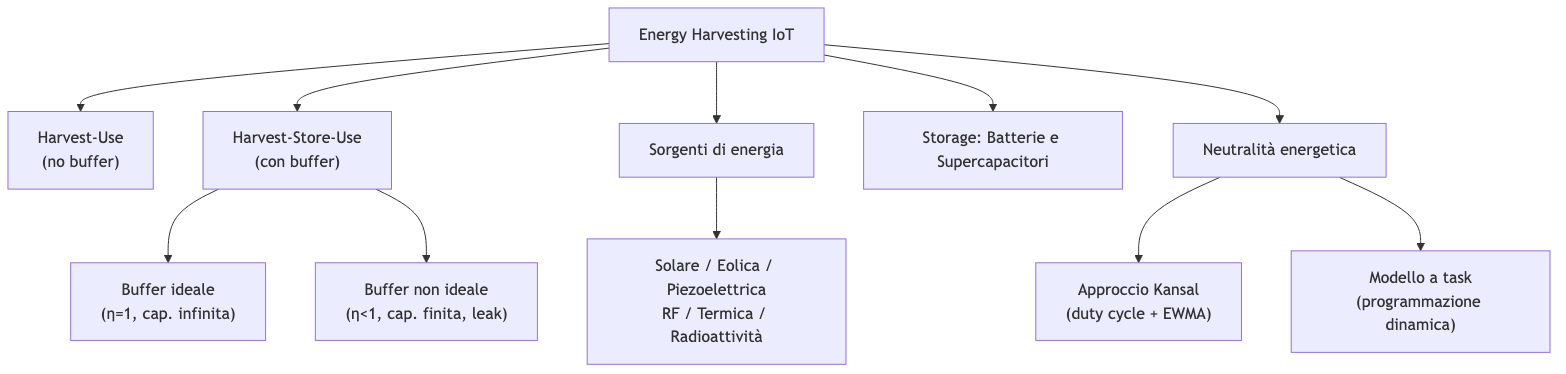
\includegraphics[keepaspectratio]{images/mermaid-lezione-24-energy-harvesting-iot-03.png}}
\caption{Mappa concettuale della lezione.}
\end{figure}

\newpage

\chapter{Kansal's Problem: Energy Neutrality nei Sistemi
IoT}\label{kansals-problem-energy-neutrality-nei-sistemi-iot}

\section{Il Contesto del Problema}\label{il-contesto-del-problema}

Il problema di \textbf{energy management} per dispositivi IoT alimentati
da sorgenti rinnovabili è intrinsecamente legato alla natura della
sorgente di energia. Kansal considera il caso di sorgenti
\textbf{prevedibili ma non controllabili}: fonti come l'energia solare
sono soggette a variazioni giornaliere e stagionali, ma il loro
andamento nel tempo può essere stimato con buona precisione. L'approccio
non si estende a sorgenti imprevedibili (problema troppo difficile,
impossibile garantire performance) né a sorgenti controllabili (problema
banale: basta produrre energia su richiesta).

L'obiettivo del power management è triplice: - mantenere il sistema
\textbf{energy neutral}, cioè fare in modo che la batteria non si
esaurisca mai; - \textbf{evitare che il dispositivo si spenga} prima del
prossimo ciclo di ricarica; - \textbf{massimizzare le prestazioni} del
nodo, ossia la sua utility.

L'approccio consiste nel tener conto del livello attuale e atteso della
batteria, modulare dinamicamente le prestazioni del dispositivo (e
quindi il carico energetico), garantendo che il dispositivo non scenda
sotto le performance minime.

\begin{center}\rule{0.5\linewidth}{0.5pt}\end{center}

\section{Modello Formale: le Due
Condizioni}\label{modello-formale-le-due-condizioni}

\subsection{Condizione 1 --- Produzione di
Energia}\label{condizione-1-produzione-di-energia}

La quantità totale di energia prodotta nell'intervallo \([0, T]\) è
definita come:

\[
E_T = \int_T P_s(t) \, dt
\]

dove \(P_s(t)\) è la potenza istantanea della sorgente. Kansal assume
che questa quantità sia \textbf{bounded} da un corridoio lineare:
esistono due costanti reali \(\rho_s\) e \(\sigma\) tali che:

\[
\rho_s \cdot T - \sigma \leq E_T \leq \rho_s \cdot T + \sigma
\]

Il parametro \(\rho_s\) rappresenta il \textbf{trend medio} di
produzione (la pendenza), mentre \(\sigma\) è il \textbf{burst bound}
che cattura la variabilità a breve termine attorno alla retta di
tendenza.

\begin{figure}
\centering
\pandocbounded{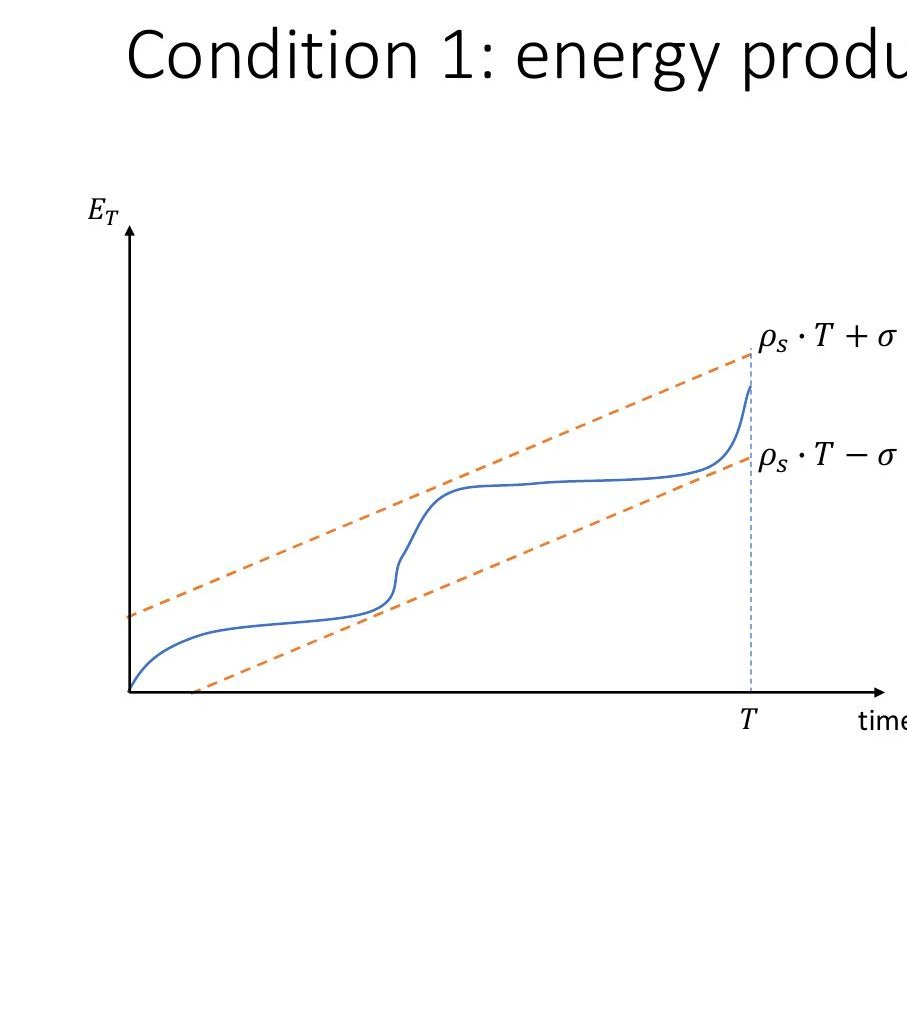
\includegraphics[keepaspectratio]{images/lezione-28-kansal-problem-e-energy-neutrality-img-01.jpg}}
\caption{1 --- La curva blu mostra l'energia prodotta cumulativa \(E_T\)
che oscilla tra le due rette tratteggiate \(\rho_s T \pm \sigma\).}
\end{figure}

\subsection{Condizione 2 --- Consumo
(Load)}\label{condizione-2-consumo-load}

Analogamente, il consumo totale \(L_T\) nell'intervallo \([0, T]\) è:

\[
L_T = \int_T P_c(t) \, dt
\]

e si assume anch'esso bounded (da sopra) da una retta lineare
parametrizzata da \(\rho_c\) e \(\delta\):

\[
0 \leq L_T \leq \rho_c \cdot T + \delta
\]

Il consumo può essere modulato dal sistema (è una variabile
controllata), mentre la produzione è data dalla natura.

\begin{figure}
\centering
\pandocbounded{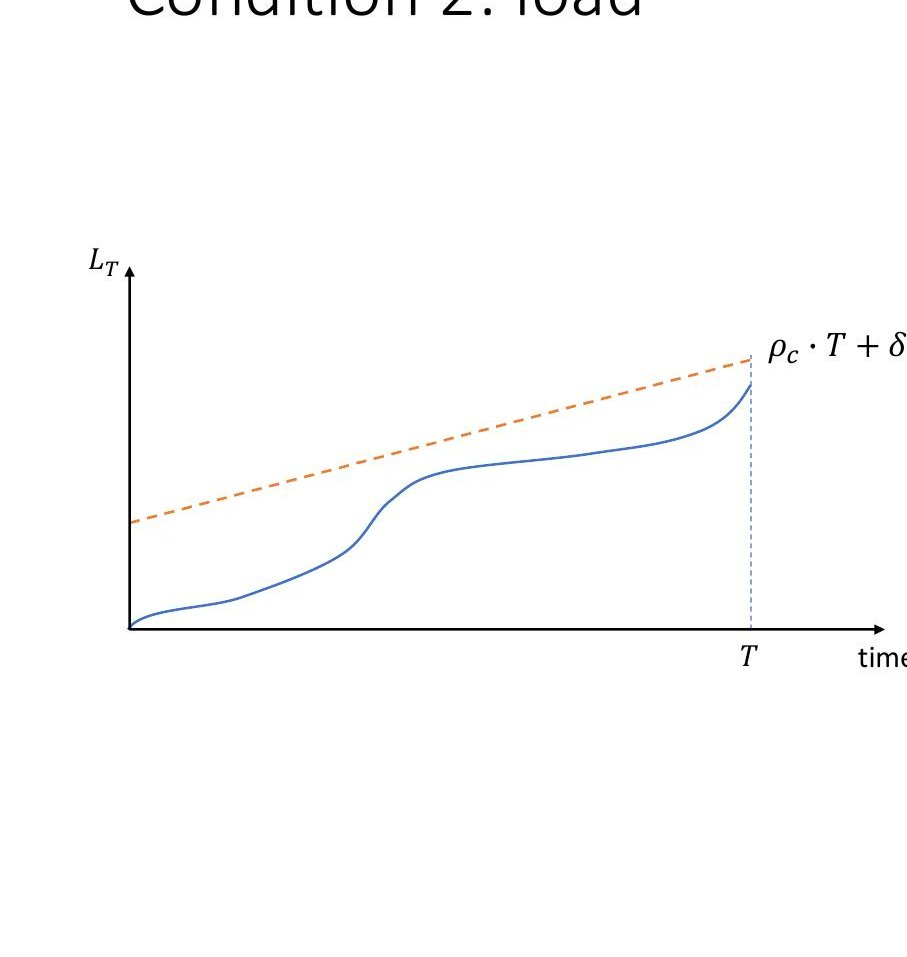
\includegraphics[keepaspectratio]{images/lezione-28-kansal-problem-e-energy-neutrality-img-02.jpg}}
\caption{2 --- Il consumo cumulativo \(L_T\) rimane al di sotto della
retta \(\rho_c T + \delta\).}
\end{figure}

\begin{center}\rule{0.5\linewidth}{0.5pt}\end{center}

\section{Il Teorema di Kansal}\label{il-teorema-di-kansal}

\begin{callouttheorem}{Condizione sufficiente per Energy Neutrality}

Se le assunzioni sulle condizioni 1 e 2 valgono, e la batteria è
caratterizzata da: - \textbf{efficienza di carica} \(\eta\) (frazione
dell'energia prodotta effettivamente immagazzinata) - \textbf{leakage}
\(\rho_{leak}\) (perdita di energia per autoscarica)

allora una condizione \textbf{sufficiente} per la neutralità energetica
del sistema è:

\[
\begin{cases}
\eta \rho_s \geq \rho_c + \rho_{leak} \\
B_0 \geq \eta\sigma + \delta \\
B_{max} \geq B_0
\end{cases}
\]

Le tre condizioni garantiscono rispettivamente che: (1) il trend di
produzione (con efficienza) superi il trend di consumo più la perdita;
(2) la carica iniziale sia sufficiente nel caso peggiore; (3) la carica
iniziale richiesta sia ammissibile rispetto alla capacità massima.

\end{callouttheorem}

\begin{center}\rule{0.5\linewidth}{0.5pt}\end{center}

\section{Utility e Duty Cycle}\label{utility-e-duty-cycle}

L'approccio pratico di Kansal per soddisfare la condizione 2 è modulare
il \textbf{duty cycle} del dispositivo. Ridurre il duty cycle riduce il
consumo energetico (relazione quasi lineare), ma un duty cycle del 0\%
non ha senso operativo. Si definisce quindi una funzione di
\textbf{utility} \(u(dc)\) che misura il valore applicativo del duty
cycle:

\[
u(dc) = \begin{cases}
0 & \text{se } dc < dc_{min} \\
\alpha \cdot dc + \beta & \text{se } dc_{min} \leq dc \leq dc_{max} \\
u_M & \text{se } dc > dc_{max}
\end{cases}
\]

La funzione è piatta a zero sotto \(dc_{min}\) (il dispositivo non
funziona abbastanza bene da essere utile), lineare nella zona operativa,
e satura a \(u_M\) sopra \(dc_{max}\) (aumentare il duty cycle non porta
ulteriori benefici). Il sistema quindi non vuole azzerare il consumo, ma
trovare un duty cycle che massimizzi l'utility pur rimanendo energy
neutral.

\begin{figure}
\centering
\pandocbounded{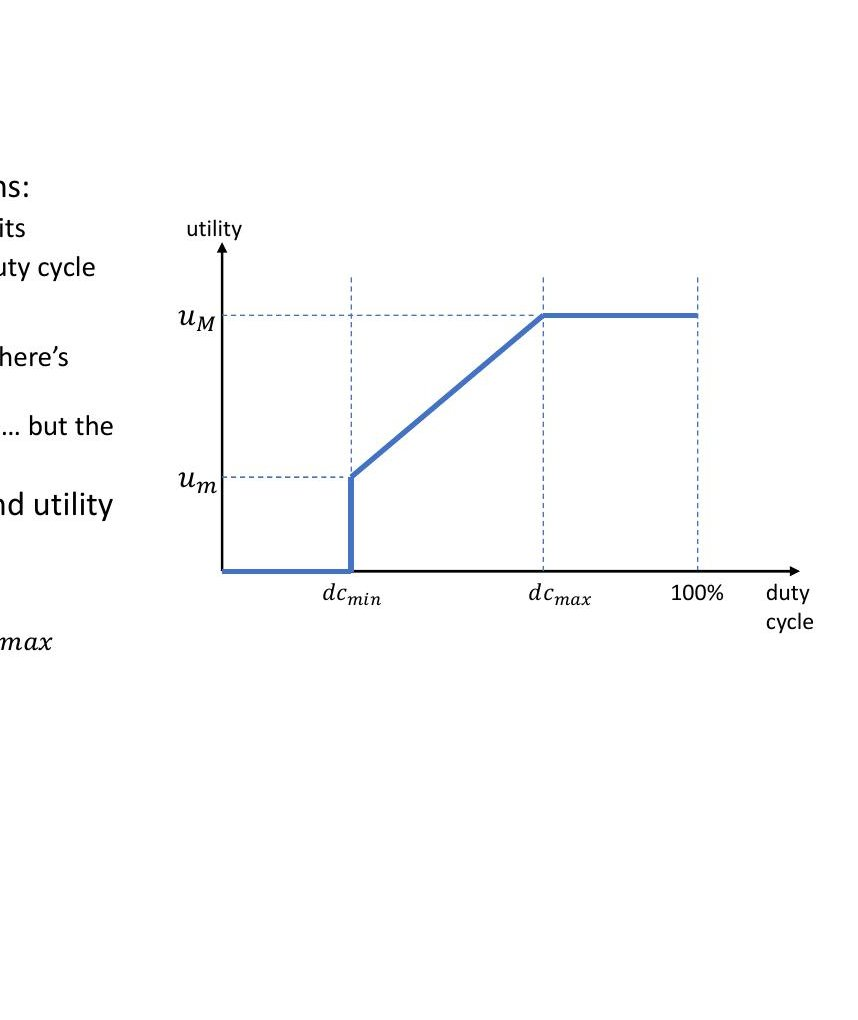
\includegraphics[keepaspectratio]{images/lezione-28-kansal-problem-e-energy-neutrality-img-03.jpg}}
\caption{3 --- La funzione \(u(dc)\): segmento piatto a \(u_m\), rampa
lineare, plateau a \(u_M\).}
\end{figure}

\begin{callouttip}{Calcolo dei parametri α e β}

Dati: \(dc_{max} = 90\%\), \(dc_{min} = 50\%\), \(u_M = 100\),
\(u_m = 10\).

\[
\alpha = \frac{u_M - u_m}{dc_{max} - dc_{min}} = \frac{90}{40} = 2.25
\]

\[
\beta = u_m - \alpha \cdot dc_{min} = 10 - 2.25 \cdot 50 = -102.5
\]

Quindi: \(u(dc) = 2.25 \cdot dc - 102.5\) nella zona lineare.

\end{callouttip}

Analogamente, se il consumo di potenza è lineare nel duty cycle ---
\(p(dc) = \rho \cdot dc + \sigma\) --- e si conoscono \(p_{max}\) e
\(p_{min}\) corrispondenti a \(dc_{max}\) e \(dc_{min}\):

\[
\rho = \frac{p_{max} - p_{min}}{dc_{max} - dc_{min}} = \frac{4}{40} = 0.1, \quad \sigma = p_{min} - \rho \cdot dc_{min} = -4
\]

Con i valori dell'esempio (\(p_{max} = 5\,\text{mA}\),
\(p_{min} = 1\,\text{mA}\)): \(p(dc) = 0.1 \cdot dc - 4\).

\begin{callouttip}{Esempio applicativo}

In un sistema di rilevamento di intrusi: campionare a frequenza più alta
aumenta la capacità di rilevamento (utility alta), ma sotto una soglia
minima il campionamento è troppo rado per essere utile. Sopra una soglia
massima, l'intruso è comunque lento abbastanza da essere rilevato ---
ulteriore sampling è spreco.

\end{callouttip}

\begin{center}\rule{0.5\linewidth}{0.5pt}\end{center}

\section{Il Problema di
Ottimizzazione}\label{il-problema-di-ottimizzazione}

Il sistema è descrito da tre grandezze che variano nel tempo in modo
interdipendente: - la \textbf{produzione} varia in modo non controllato
ma prevedibile; - il \textbf{carico} varia in funzione del duty cycle
(controllato); - la \textbf{carica della batteria} varia di conseguenza.

L'obiettivo è trovare l'assegnamento di duty cycle che massimizzi
l'utility totale mantenendo la neutralità energetica.

\subsection{Discretizzazione
Temporale}\label{discretizzazione-temporale}

Invece di lavorare in continuo, Kansal discretizza il tempo in
\textbf{slot} (tipicamente 24 slot di 1 ora per una giornata). Questo
semplifica lo scheduling e rende il sistema più stabile: si assegna un
duty cycle per slot, lo scheduler gira una volta al giorno (es. a
mezzanotte), e le previsioni meteorologiche forniscono le stime di
produzione per ogni slot.

\begin{center}\rule{0.5\linewidth}{0.5pt}\end{center}

\section{Previsione della Produzione:
EWMA}\label{previsione-della-produzione-ewma}

Per stimare la produzione futura, Kansal adotta un filtro \textbf{EWMA}
(Exponentially Weighted Moving Average, \emph{media mobile
esponenzialmente pesata}): l'ipotesi è che la produzione nello stesso
slot del giorno successivo sarà simile a quella del giorno corrente.

Definendo \(p_j(i)\) la produzione misurata nello slot \(i\) del giorno
\(j\), e \(\tilde{p}_j(i)\) la produzione stimata, la previsione per il
giorno successivo è:

\[
\tilde{p}_{j+1}(i) = \alpha \cdot p_j(i) + (1 - \alpha) \cdot \tilde{p}_j(i)
\]

con \(\alpha < 1\) parametro (costante o adattivo). La stima è dunque
una media pesata della misura più recente e della stima precedente: più
\(\alpha\) è vicino a 1, maggior peso si dà alla misura più recente.

\begin{calloutnote}{Esperimenti con Heliomote}

Gli esperimenti di Kansal su nodi sensori reali con pannello solare (un
cosiddetto ``Heliomote'') mostrano che: la produzione giornaliera ha un
profilo a campana centrato a mezzogiorno, l'errore EWMA è basso nelle
ore notturne e massimo attorno a mezzogiorno (maggiore variabilità), e
la produzione è altamente ripetibile giorno dopo giorno.

\end{calloutnote}

\begin{figure}
\centering
\pandocbounded{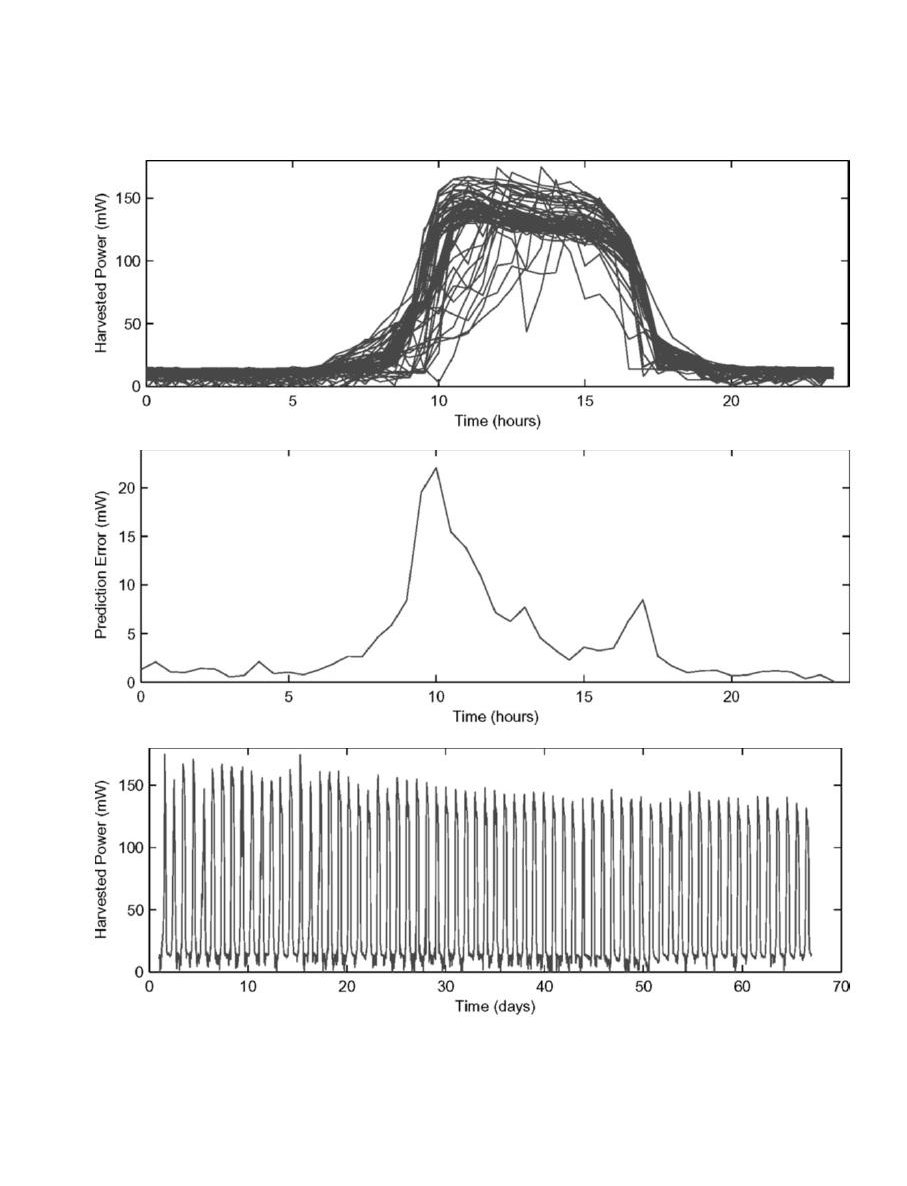
\includegraphics[keepaspectratio]{images/lezione-28-kansal-problem-e-energy-neutrality-img-04.jpg}}
\caption{4 --- Dall'alto: (1) profili di produzione giornaliera
sovrapposti per molti giorni; (2) errore del predittore EWMA; (3)
energia raccolta su 70 giorni consecutivi con ciclo giorno/notte
visibile.}
\end{figure}

\begin{center}\rule{0.5\linewidth}{0.5pt}\end{center}

\section{L'Algoritmo di Kansal}\label{lalgoritmo-di-kansal}

L'algoritmo assegna il duty cycle a ogni slot in base alla produzione
attesa \(\tilde{p}_s(i)\). Supponiamo di conoscere \(p_{max}\) (consumo
al duty cycle massimo) e \(p_{min}\) (consumo al duty cycle minimo). Si
definiscono due insiemi di slot:

\[
S = \{i : \tilde{p}_s(i) \geq p_{max}\} \quad \text{(slot "di sole" — produzione abbondante)}
\] \[
D = \{i : \tilde{p}_s(i) < p_{max}\} \quad \text{(slot "bui" — produzione insufficiente)}
\]

\textbf{Prima assegnazione (soluzione iniziale):}

\begin{verbatim}
// Step 1: assegnamento iniziale
for each slot i:
    if i ∈ S:
        dc_i = dc_max   // massimo duty cycle nei sun slot
    else:
        dc_i = dc_min   // minimo duty cycle nei dark slot
\end{verbatim}

A questo punto si calcola il \textbf{surplus residuo}
\(p_{res} = B(k+1) - B(1)\):

\subsection{\texorpdfstring{Caso 1 --- Sovraproduzione
(\(p_{res} > 0\))}{Caso 1 --- Sovraproduzione (p\_\{res\} \textgreater{} 0)}}\label{caso-1-sovraproduzione-p_res-0}

C'è energia avanzata alla fine del giorno. L'algoritmo la usa per alzare
il duty cycle in alcuni dark slot, partendo da quelli con indice più
piccolo:

\begin{Shaded}
\begin{Highlighting}[]
\CommentTok{// p\_res \textgreater{} 0: surplus di energia}
\CommentTok{// p\_diff = p\_max {-} p\_min (differenza di consumo tra dc\_max e dc\_min)}

\ControlFlowTok{while} \OperatorTok{(}\NormalTok{p\_res }\OperatorTok{\textgreater{}}\NormalTok{ p\_diff}\OperatorTok{)} \OperatorTok{\{}
    \CommentTok{// prendi il dark slot con indice minore (ancora a dc\_min)}
\NormalTok{    let i }\OperatorTok{=}\NormalTok{ min\_index}\OperatorTok{(}\NormalTok{D with dc\_i }\OperatorTok{==}\NormalTok{ dc\_min}\OperatorTok{);}
\NormalTok{    dc\_i }\OperatorTok{=}\NormalTok{ dc\_max}\OperatorTok{;}
\NormalTok{    p\_res }\OperatorTok{{-}=}\NormalTok{ p\_diff}\OperatorTok{;}
\OperatorTok{\}}

\ControlFlowTok{if} \OperatorTok{(}\NormalTok{p\_res }\OperatorTok{\textgreater{}} \DecValTok{0}\OperatorTok{)} \OperatorTok{\{}
    \CommentTok{// p\_res non basta per un altro slot al massimo:}
    \CommentTok{// alza parzialmente il dc del prossimo slot}
\NormalTok{    let i }\OperatorTok{=}\NormalTok{ min\_index}\OperatorTok{(}\NormalTok{D with dc\_i }\OperatorTok{==}\NormalTok{ dc\_min}\OperatorTok{);}
\NormalTok{    dc\_i }\OperatorTok{=}\NormalTok{ DutyCycle}\OperatorTok{(}\NormalTok{p\_min }\OperatorTok{+}\NormalTok{ p\_res}\OperatorTok{);}
    \CommentTok{// DutyCycle(p) = (p {-} sigma) / rho  [inversa di p(dc)]}
\OperatorTok{\}}
\end{Highlighting}
\end{Shaded}

\subsection{\texorpdfstring{Caso 2 --- Sottoproduzione
(\(p_{res} < 0\))}{Caso 2 --- Sottoproduzione (p\_\{res\} \textless{} 0)}}\label{caso-2-sottoproduzione-p_res-0}

Manca energia alla fine del giorno. L'algoritmo riduce uniformemente il
duty cycle in tutti i sun slot per compensare:

\begin{Shaded}
\begin{Highlighting}[]
\CommentTok{// p\_res \textless{} 0: underproduction}
\CommentTok{// |S| = numero di sun slot}

\ControlFlowTok{if} \OperatorTok{((}\NormalTok{p\_max }\OperatorTok{{-}}\NormalTok{ p\_min}\OperatorTok{)} \OperatorTok{/} \OperatorTok{|}\NormalTok{S}\OperatorTok{|} \OperatorTok{\textless{}}\NormalTok{ abs}\OperatorTok{(}\NormalTok{p\_res}\OperatorTok{)} \OperatorTok{/} \OperatorTok{|}\NormalTok{S}\OperatorTok{|)} \OperatorTok{\{}
    \ControlFlowTok{return} \OperatorTok{{-}}\DecValTok{1}\OperatorTok{;}  \CommentTok{// impossibile: anche riducendo tutti i sun slot non basta}
\OperatorTok{\}}

\ControlFlowTok{for}\NormalTok{ each i ∈ S }\OperatorTok{\{}
    \CommentTok{// abbassa il dc di ogni sun slot della stessa quantità}
\NormalTok{    dc\_i }\OperatorTok{=}\NormalTok{ DutyCycle}\OperatorTok{(}\NormalTok{p\_max }\OperatorTok{{-}}\NormalTok{ abs}\OperatorTok{(}\NormalTok{p\_res}\OperatorTok{)} \OperatorTok{/} \OperatorTok{|}\NormalTok{S}\OperatorTok{|);}
\OperatorTok{\}}
\end{Highlighting}
\end{Shaded}

La riduzione è uniforme per mantenere equità tra le ore di luce.

\begin{callouttip}{Proprietà dell’algoritmo}

\begin{itemize}
\tightlist
\item
  \textbf{Ottimalità}: la soluzione prodotta è ottimale per il problema
  di massimizzazione dell'utility.
\item
  \textbf{Semplicità}: nessun solver di programmazione lineare richiesto
  --- solo confronti e operazioni aritmetiche.
\item
  \textbf{Memoria ridotta}: adatto a processori a bassa potenza.
\item
  \textbf{Adattamento dinamico}: se la produzione reale si discosta
  significativamente dalla previsione durante la giornata, il ciclo di
  ottimizzazione viene rieseguito per i restanti slot con la stessa
  logica.
\end{itemize}

\end{callouttip}

\begin{calloutwarning}{Limiti dell’algoritmo di Kansal}

\begin{itemize}
\tightlist
\item
  Basato su \textbf{scaling lineare del duty cycle}: le frequenze di
  campionamento risultanti sono in genere irregolari, il che può essere
  problematico per alcune applicazioni (es. serie temporali con
  campionamento non uniforme).
\item
  Modella solo la modulazione del duty cycle: \textbf{non è adatto} a
  scenari con scelte tra trasduttori alternativi, algoritmi di
  elaborazione diversi, o comportamenti più complessi.
\end{itemize}

\end{calloutwarning}

\begin{center}\rule{0.5\linewidth}{0.5pt}\end{center}

\section{Esercizio Risolto --- Esercizio
1}\label{esercizio-risolto-esercizio-1}

\begin{callouttip}{Esercizio 1}

Dati: \(dc_{max}=90\%\), \(p_{max}=5\,\text{mA}\), \(u(dc_{max})=100\);
\(dc_{min}=50\%\), \(p_{min}=1\,\text{mA}\), \(u(dc_{min})=10\).

Dalle formule già calcolate:
\[p(dc) = 0.1 \cdot dc - 4, \quad u(dc) = 2.25 \cdot dc - 102.5\]

Produzione per slot:
\(\tilde{p}_s = [0, 0, 0, 2, 6, 11, 10, 7, 3, 0, 0, 0]\).

\end{callouttip}

\textbf{Step 1 --- Assegnamento iniziale:}

\(S = \{5, 6, 7, 8\}\) (produzione \(\geq p_{max} = 5\)),
\(D = \{1,2,3,4,9,10,11,12\}\).

{\def\LTcaptype{none} % do not increment counter
\begin{longtable}[]{@{}
  >{\raggedright\arraybackslash}p{(\linewidth - 24\tabcolsep) * \real{0.1304}}
  >{\raggedright\arraybackslash}p{(\linewidth - 24\tabcolsep) * \real{0.0652}}
  >{\raggedright\arraybackslash}p{(\linewidth - 24\tabcolsep) * \real{0.0652}}
  >{\raggedright\arraybackslash}p{(\linewidth - 24\tabcolsep) * \real{0.0652}}
  >{\raggedright\arraybackslash}p{(\linewidth - 24\tabcolsep) * \real{0.0652}}
  >{\raggedright\arraybackslash}p{(\linewidth - 24\tabcolsep) * \real{0.0652}}
  >{\raggedright\arraybackslash}p{(\linewidth - 24\tabcolsep) * \real{0.0652}}
  >{\raggedright\arraybackslash}p{(\linewidth - 24\tabcolsep) * \real{0.0652}}
  >{\raggedright\arraybackslash}p{(\linewidth - 24\tabcolsep) * \real{0.0652}}
  >{\raggedright\arraybackslash}p{(\linewidth - 24\tabcolsep) * \real{0.0652}}
  >{\raggedright\arraybackslash}p{(\linewidth - 24\tabcolsep) * \real{0.0870}}
  >{\raggedright\arraybackslash}p{(\linewidth - 24\tabcolsep) * \real{0.0870}}
  >{\raggedright\arraybackslash}p{(\linewidth - 24\tabcolsep) * \real{0.1087}}@{}}
\toprule\noalign{}
\begin{minipage}[b]{\linewidth}\raggedright
Slot
\end{minipage} & \begin{minipage}[b]{\linewidth}\raggedright
1
\end{minipage} & \begin{minipage}[b]{\linewidth}\raggedright
2
\end{minipage} & \begin{minipage}[b]{\linewidth}\raggedright
3
\end{minipage} & \begin{minipage}[b]{\linewidth}\raggedright
4
\end{minipage} & \begin{minipage}[b]{\linewidth}\raggedright
5
\end{minipage} & \begin{minipage}[b]{\linewidth}\raggedright
6
\end{minipage} & \begin{minipage}[b]{\linewidth}\raggedright
7
\end{minipage} & \begin{minipage}[b]{\linewidth}\raggedright
8
\end{minipage} & \begin{minipage}[b]{\linewidth}\raggedright
9
\end{minipage} & \begin{minipage}[b]{\linewidth}\raggedright
10
\end{minipage} & \begin{minipage}[b]{\linewidth}\raggedright
11
\end{minipage} & \begin{minipage}[b]{\linewidth}\raggedright
12
\end{minipage} \\
\midrule\noalign{}
\endhead
\bottomrule\noalign{}
\endlastfoot
\(\tilde{p}_s(i)\) & 0 & 0 & 0 & 2 & 6 & 11 & 10 & 7 & 3 & 0 & 0 & 0 \\
\(dc_i\) & 50 & 50 & 50 & 50 & 90 & 90 & 90 & 90 & 50 & 50 & 50 & 50 \\
\(u(\cdot)\) & 10 & 10 & 10 & 10 & 100 & 100 & 100 & 100 & 10 & 10 & 10
& 10 \\
\(p(\cdot)\) & 1 & 1 & 1 & 1 & 5 & 5 & 5 & 5 & 1 & 1 & 1 & 1 \\
\end{longtable}
}

Totale prodotto: 39. Totale consumato: \(8 \times 1 + 4 \times 5 = 28\).
\textbf{Surplus \(p_{res} = 11 > 0\) → Caso 1.}

\textbf{Step 2 --- Uso del surplus:}

\(p_{diff} = 5 - 1 = 4\). Con \(p_{res} = 11\): si possono portare
\(\lfloor 11/4 \rfloor = 2\) dark slot al massimo (slot 1 e 2).
\(p_{res}\) residuo: \(11 - 8 = 3\).

\textbf{Step 3 --- Residuo parziale:}

\(p_{res} = 3 < 4\). Prossimo dark slot: slot 3. Nuovo consumo:
\(p_{min} + p_{res} = 1 + 3 = 4\).
\[dc = \frac{p - \sigma}{\rho} = \frac{4 + 4}{0.1} = 80\%, \quad u(80) = 2.25 \cdot 80 - 102.5 = 77.5\]

\textbf{Soluzione finale:}

{\def\LTcaptype{none} % do not increment counter
\begin{longtable}[]{@{}
  >{\raggedright\arraybackslash}p{(\linewidth - 24\tabcolsep) * \real{0.1304}}
  >{\raggedright\arraybackslash}p{(\linewidth - 24\tabcolsep) * \real{0.0652}}
  >{\raggedright\arraybackslash}p{(\linewidth - 24\tabcolsep) * \real{0.0652}}
  >{\raggedright\arraybackslash}p{(\linewidth - 24\tabcolsep) * \real{0.0652}}
  >{\raggedright\arraybackslash}p{(\linewidth - 24\tabcolsep) * \real{0.0652}}
  >{\raggedright\arraybackslash}p{(\linewidth - 24\tabcolsep) * \real{0.0652}}
  >{\raggedright\arraybackslash}p{(\linewidth - 24\tabcolsep) * \real{0.0652}}
  >{\raggedright\arraybackslash}p{(\linewidth - 24\tabcolsep) * \real{0.0652}}
  >{\raggedright\arraybackslash}p{(\linewidth - 24\tabcolsep) * \real{0.0652}}
  >{\raggedright\arraybackslash}p{(\linewidth - 24\tabcolsep) * \real{0.0652}}
  >{\raggedright\arraybackslash}p{(\linewidth - 24\tabcolsep) * \real{0.0870}}
  >{\raggedright\arraybackslash}p{(\linewidth - 24\tabcolsep) * \real{0.0870}}
  >{\raggedright\arraybackslash}p{(\linewidth - 24\tabcolsep) * \real{0.1087}}@{}}
\toprule\noalign{}
\begin{minipage}[b]{\linewidth}\raggedright
Slot
\end{minipage} & \begin{minipage}[b]{\linewidth}\raggedright
1
\end{minipage} & \begin{minipage}[b]{\linewidth}\raggedright
2
\end{minipage} & \begin{minipage}[b]{\linewidth}\raggedright
3
\end{minipage} & \begin{minipage}[b]{\linewidth}\raggedright
4
\end{minipage} & \begin{minipage}[b]{\linewidth}\raggedright
5
\end{minipage} & \begin{minipage}[b]{\linewidth}\raggedright
6
\end{minipage} & \begin{minipage}[b]{\linewidth}\raggedright
7
\end{minipage} & \begin{minipage}[b]{\linewidth}\raggedright
8
\end{minipage} & \begin{minipage}[b]{\linewidth}\raggedright
9
\end{minipage} & \begin{minipage}[b]{\linewidth}\raggedright
10
\end{minipage} & \begin{minipage}[b]{\linewidth}\raggedright
11
\end{minipage} & \begin{minipage}[b]{\linewidth}\raggedright
12
\end{minipage} \\
\midrule\noalign{}
\endhead
\bottomrule\noalign{}
\endlastfoot
\(\tilde{p}_s(i)\) & 0 & 0 & 0 & 2 & 6 & 11 & 10 & 7 & 3 & 0 & 0 & 0 \\
\(dc_i\) & \textbf{90} & \textbf{90} & \textbf{80} & 50 & 90 & 90 & 90 &
90 & 50 & 50 & 50 & 50 \\
\(u(\cdot)\) & \textbf{100} & \textbf{100} & \textbf{77.5} & 10 & 100 &
100 & 100 & 100 & 10 & 10 & 10 & 10 \\
\(p(\cdot)\) & \textbf{5} & \textbf{5} & \textbf{4} & 1 & 5 & 5 & 5 & 5
& 1 & 1 & 1 & 1 \\
\end{longtable}
}

\begin{center}\rule{0.5\linewidth}{0.5pt}\end{center}

\section{Esercizio Risolto --- Esercizio
2}\label{esercizio-risolto-esercizio-2}

\begin{callouttip}{Esercizio 2 (variante con p\_\{min\} = 2\\,\\text\{mA\})}

Dati: \(dc_{max}=90\%\), \(p_{max}=5\,\text{mA}\); \(dc_{min}=50\%\),
\(p_{min}=2\,\text{mA}\).

Nuove formule:
\[\rho = \frac{5-2}{90-50} = 0.075, \quad \sigma = 2 - 0.075 \cdot 50 = -1.75\]
\[p(dc) = 0.075 \cdot dc - 1.75, \quad u(dc) = 2.25 \cdot dc - 102.5 \text{ (invariata)}\]

Produzione per slot:
\(\tilde{p}_s = [0, 0, 1, 3, 5, 8, 4, 3, 2, 0, 0, 0]\).

\end{callouttip}

\textbf{Step 1 --- Assegnamento iniziale:}

\(S = \{5, 6\}\) (produzione \(\geq 5\)),
\(D = \{1,2,3,4,7,8,9,10,11,12\}\).

{\def\LTcaptype{none} % do not increment counter
\begin{longtable}[]{@{}
  >{\raggedright\arraybackslash}p{(\linewidth - 24\tabcolsep) * \real{0.1304}}
  >{\raggedright\arraybackslash}p{(\linewidth - 24\tabcolsep) * \real{0.0652}}
  >{\raggedright\arraybackslash}p{(\linewidth - 24\tabcolsep) * \real{0.0652}}
  >{\raggedright\arraybackslash}p{(\linewidth - 24\tabcolsep) * \real{0.0652}}
  >{\raggedright\arraybackslash}p{(\linewidth - 24\tabcolsep) * \real{0.0652}}
  >{\raggedright\arraybackslash}p{(\linewidth - 24\tabcolsep) * \real{0.0652}}
  >{\raggedright\arraybackslash}p{(\linewidth - 24\tabcolsep) * \real{0.0652}}
  >{\raggedright\arraybackslash}p{(\linewidth - 24\tabcolsep) * \real{0.0652}}
  >{\raggedright\arraybackslash}p{(\linewidth - 24\tabcolsep) * \real{0.0652}}
  >{\raggedright\arraybackslash}p{(\linewidth - 24\tabcolsep) * \real{0.0652}}
  >{\raggedright\arraybackslash}p{(\linewidth - 24\tabcolsep) * \real{0.0870}}
  >{\raggedright\arraybackslash}p{(\linewidth - 24\tabcolsep) * \real{0.0870}}
  >{\raggedright\arraybackslash}p{(\linewidth - 24\tabcolsep) * \real{0.1087}}@{}}
\toprule\noalign{}
\begin{minipage}[b]{\linewidth}\raggedright
Slot
\end{minipage} & \begin{minipage}[b]{\linewidth}\raggedright
1
\end{minipage} & \begin{minipage}[b]{\linewidth}\raggedright
2
\end{minipage} & \begin{minipage}[b]{\linewidth}\raggedright
3
\end{minipage} & \begin{minipage}[b]{\linewidth}\raggedright
4
\end{minipage} & \begin{minipage}[b]{\linewidth}\raggedright
5
\end{minipage} & \begin{minipage}[b]{\linewidth}\raggedright
6
\end{minipage} & \begin{minipage}[b]{\linewidth}\raggedright
7
\end{minipage} & \begin{minipage}[b]{\linewidth}\raggedright
8
\end{minipage} & \begin{minipage}[b]{\linewidth}\raggedright
9
\end{minipage} & \begin{minipage}[b]{\linewidth}\raggedright
10
\end{minipage} & \begin{minipage}[b]{\linewidth}\raggedright
11
\end{minipage} & \begin{minipage}[b]{\linewidth}\raggedright
12
\end{minipage} \\
\midrule\noalign{}
\endhead
\bottomrule\noalign{}
\endlastfoot
\(\tilde{p}_s(i)\) & 0 & 0 & 1 & 3 & 5 & 8 & 4 & 3 & 2 & 0 & 0 & 0 \\
\(dc_i\) & 50 & 50 & 50 & 50 & 90 & 90 & 50 & 50 & 50 & 50 & 50 & 50 \\
\(u(\cdot)\) & 10 & 10 & 10 & 10 & 100 & 100 & 10 & 10 & 10 & 10 & 10 &
10 \\
\(p(\cdot)\) & 2 & 2 & 2 & 2 & 5 & 5 & 2 & 2 & 2 & 2 & 2 & 2 \\
\end{longtable}
}

Totale prodotto: 26. Totale consumato:
\(10 \times 2 + 2 \times 5 = 30\). \textbf{\(p_{res} = -4 < 0\) → Caso
2.}

\textbf{Step 2 --- Caso 2:}

\(|S| = 2\). Verifica ammissibilità:
\((p_{max} - p_{min})/|S| = 3/2 = 1.5\). \(|p_{res}|/|S| = 2\). Poiché
\(1.5 < 2\)\ldots{} attenzione: la verifica dell'algoritmo è
\((p_{max} - p_{min})/|S| < |p_{res}|\) (non diviso \(|S|\)).
\((5-2)/2 = 1.5 < 4\): la condizione di inammissibilità \textbf{non
scatta}. L'algoritmo è ammissibile.

Per ogni sun slot: abbasso il consumo di \(|p_{res}|/|S| = 4/2 = 2\)
unità. Nuovo consumo per sun slot: \(p_{max} - 2 = 3\).
\[dc = \frac{3 + 1.75}{0.075} = \frac{4.75}{0.075} = 63.3\% \approx 63\%\]
\[u(63.3) = 2.25 \cdot 63.3 - 102.5 = 42.4\]

\begin{calloutnote}{Nota sulla soluzione delle slide}

Le slide approssimano a \(dc = 70\%\) (arrotondamento). Con
\(dc = 70\%\): \(p = 0.075 \cdot 70 - 1.75 = 3.5\,\text{mA}\),
\(u = 2.25 \cdot 70 - 102.5 = 55\). Questa non è un'approssimazione
accurata del caso 2 (produce un residuo di \(-1\) invece di 0). Il
calcolo esatto dà \(dc = 63.3\%\).

\end{calloutnote}

\textbf{Soluzione finale (esatta):}

{\def\LTcaptype{none} % do not increment counter
\begin{longtable}[]{@{}
  >{\raggedright\arraybackslash}p{(\linewidth - 24\tabcolsep) * \real{0.1304}}
  >{\raggedright\arraybackslash}p{(\linewidth - 24\tabcolsep) * \real{0.0652}}
  >{\raggedright\arraybackslash}p{(\linewidth - 24\tabcolsep) * \real{0.0652}}
  >{\raggedright\arraybackslash}p{(\linewidth - 24\tabcolsep) * \real{0.0652}}
  >{\raggedright\arraybackslash}p{(\linewidth - 24\tabcolsep) * \real{0.0652}}
  >{\raggedright\arraybackslash}p{(\linewidth - 24\tabcolsep) * \real{0.0652}}
  >{\raggedright\arraybackslash}p{(\linewidth - 24\tabcolsep) * \real{0.0652}}
  >{\raggedright\arraybackslash}p{(\linewidth - 24\tabcolsep) * \real{0.0652}}
  >{\raggedright\arraybackslash}p{(\linewidth - 24\tabcolsep) * \real{0.0652}}
  >{\raggedright\arraybackslash}p{(\linewidth - 24\tabcolsep) * \real{0.0652}}
  >{\raggedright\arraybackslash}p{(\linewidth - 24\tabcolsep) * \real{0.0870}}
  >{\raggedright\arraybackslash}p{(\linewidth - 24\tabcolsep) * \real{0.0870}}
  >{\raggedright\arraybackslash}p{(\linewidth - 24\tabcolsep) * \real{0.1087}}@{}}
\toprule\noalign{}
\begin{minipage}[b]{\linewidth}\raggedright
Slot
\end{minipage} & \begin{minipage}[b]{\linewidth}\raggedright
1
\end{minipage} & \begin{minipage}[b]{\linewidth}\raggedright
2
\end{minipage} & \begin{minipage}[b]{\linewidth}\raggedright
3
\end{minipage} & \begin{minipage}[b]{\linewidth}\raggedright
4
\end{minipage} & \begin{minipage}[b]{\linewidth}\raggedright
5
\end{minipage} & \begin{minipage}[b]{\linewidth}\raggedright
6
\end{minipage} & \begin{minipage}[b]{\linewidth}\raggedright
7
\end{minipage} & \begin{minipage}[b]{\linewidth}\raggedright
8
\end{minipage} & \begin{minipage}[b]{\linewidth}\raggedright
9
\end{minipage} & \begin{minipage}[b]{\linewidth}\raggedright
10
\end{minipage} & \begin{minipage}[b]{\linewidth}\raggedright
11
\end{minipage} & \begin{minipage}[b]{\linewidth}\raggedright
12
\end{minipage} \\
\midrule\noalign{}
\endhead
\bottomrule\noalign{}
\endlastfoot
\(\tilde{p}_s(i)\) & 0 & 0 & 1 & 3 & 5 & 8 & 4 & 3 & 2 & 0 & 0 & 0 \\
\(dc_i\) & 50 & 50 & 50 & 50 & \textbf{63.3} & \textbf{63.3} & 50 & 50 &
50 & 50 & 50 & 50 \\
\(u(\cdot)\) & 10 & 10 & 10 & 10 & \textbf{42.4} & \textbf{42.4} & 10 &
10 & 10 & 10 & 10 & 10 \\
\(p(\cdot)\) & 2 & 2 & 2 & 2 & \textbf{3} & \textbf{3} & 2 & 2 & 2 & 2 &
2 & 2 \\
\end{longtable}
}

\begin{center}\rule{0.5\linewidth}{0.5pt}\end{center}

\section{Modello Task-Based per la Neutralità
Energetica}\label{modello-task-based-per-la-neutralituxe0-energetica}

Kansal modella il carico tramite duty cycle, ma le applicazioni IoT
reali sono più complesse. Un'applicazione tipica esegue 4 fasi in ciclo:
\textbf{Sensing → Storing → Processing → Transmitting}. Ciascuna fase
può avere implementazioni alternative con diversi trade-off
energia/performance.

\begin{callouttip}{Alternative implementative}

\begin{itemize}
\tightlist
\item
  Scegliere tra \textbf{trasduttori diversi} (risoluzione differente,
  consumo diverso)
\item
  Disabilitare l'elaborazione locale e trasmettere i dati grezzi
  (risparmio di computazione, più traffico di rete)
\item
  Variare la frequenza di campionamento
\item
  Usare più trasduttori per aumentare l'utility
\item
  Comunicare con frequenza e affidabilità diverse
\end{itemize}

\end{callouttip}

Si chiama \textbf{task} un'implementazione specifica dell'applicazione
sul dispositivo IoT. Un dispositivo ha \(n\) task alternative, ciascuna
con costo energetico \(c_j\) e utility \(u_j\).

\subsection{Architettura del Sistema
Task-Based}\label{architettura-del-sistema-task-based}

\begin{figure}
\centering
\pandocbounded{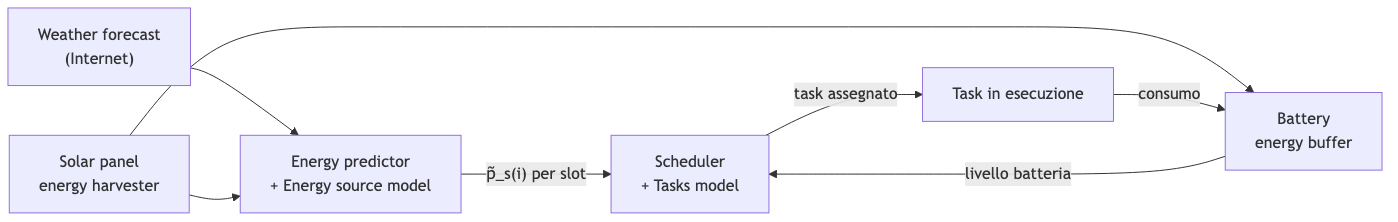
\includegraphics[keepaspectratio]{images/mermaid-lezione-28-kansal-problem-e-energy-neutrality-01.png}}
\caption{5 --- Architettura del sistema: il predittore stima la
produzione, lo scheduler assegna un task per slot ottimizzando utility e
neutralità energetica.}
\end{figure}

\subsection{Formulazione Matematica}\label{formulazione-matematica}

Tempo slottato con \(k\) slot (es. 24 ore, 1 slot/ora). Lo scheduler
assegna \textbf{esattamente un task per slot}: \(x_{i,j} = 1\) se il
task \(j\) è assegnato allo slot \(i\).

Definizioni per ogni slot \(i\): - \(\tilde{p}_s(i)\): produzione attesa
(da previsione meteorologica) - \(p_c(i)\): consumo del task assegnato
allo slot - \(p_s^+(i) = [p_s(i) - p_c(i)]^+\): eccesso di produzione →
ricarica batteria - \(p_c^-(i) = [p_c(i) - p_s(i)]^+\): deficit →
scarica batteria - \(\eta\): efficienza di carica della batteria

Il livello di batteria alla fine dello slot \(i\) è:

\[
B(i+1) = \min\{B_{max},\; B(i) + \eta \cdot p_s^+(i) - p_c^-(i)\}
\]

Il capping a \(B_{max}\) modella la saturazione della batteria.

\subsection{Problema di
Ottimizzazione}\label{problema-di-ottimizzazione}

\[
\max \sum_{i=1}^{k} \sum_{j=0}^{n} x_{i,j} \cdot u_j
\]

soggetto a:

{\def\LTcaptype{none} % do not increment counter
\begin{longtable}[]{@{}
  >{\raggedright\arraybackslash}p{(\linewidth - 2\tabcolsep) * \real{0.4091}}
  >{\raggedright\arraybackslash}p{(\linewidth - 2\tabcolsep) * \real{0.5909}}@{}}
\toprule\noalign{}
\begin{minipage}[b]{\linewidth}\raggedright
Vincolo
\end{minipage} & \begin{minipage}[b]{\linewidth}\raggedright
Significato
\end{minipage} \\
\midrule\noalign{}
\endhead
\bottomrule\noalign{}
\endlastfoot
\(\sum_j x_{i,j} = 1 \; \forall i\) & Esattamente un task per slot \\
\(B(1) \leq B(k+1)\) & Neutralità energetica \\
\(B_{min} \leq B(i) \; \forall i\) & La batteria non scende mai sotto la
soglia minima \\
\(B(i+1) = \min\{B_{max}, B(i) + \eta p_s^+(i) - p_c^-(i)\} \; \forall i\)
& Equazione di stato della batteria \\
\end{longtable}
}

\begin{center}\rule{0.5\linewidth}{0.5pt}\end{center}

\section{Soluzione con Programmazione
Dinamica}\label{soluzione-con-programmazione-dinamica}

Il problema di ottimizzazione task-based è \textbf{NP-Hard} (si riduce a
una variante del problema dello zaino). Tuttavia esiste una soluzione
\textbf{pseudo-polinomiale} basata su programmazione dinamica,
praticabile su piattaforme a bassa potenza.

\subsection{Ricorrenza}\label{ricorrenza}

Lo stato del sistema è la coppia \((i, b)\): slot corrente e livello di
batteria all'inizio di quello slot. La funzione \(opt(i, b)\) è
l'utility ottimale ottenibile dagli slot \(i\) a \(k\) partendo con
livello \(b\).

\textbf{Caso base} (ultimo slot \(k\)):

\[
opt(k, b) = \max_{j=1,\ldots,n} \{u_j : b + \eta \cdot p_s^+(k) - p_c^-(k) \geq B(1)\}
\]

Solo i task che garantiscono la neutralità energetica alla fine del
giorno (\(B(k+1) \geq B(1)\)) sono ammissibili.

\textbf{Passo ricorsivo} (slot \(i < k\)):

\[
opt(i, b) = \max_{j=1,\ldots,n} \{u_j + opt(i+1, B^j(i+1)) : B^j(i+1) \geq B_{min}\}
\]

dove \(B^j(i+1)\) è il livello di batteria residuo a fine slot \(i\) se
si assegna il task \(T_j\). La ricorsione procede \textbf{all'indietro}
dall'ultimo slot al primo (approccio backward).

\subsection{Complessità}\label{complessituxe0}

{\def\LTcaptype{none} % do not increment counter
\begin{longtable}[]{@{}ll@{}}
\toprule\noalign{}
& Complessità \\
\midrule\noalign{}
\endhead
\bottomrule\noalign{}
\endlastfoot
\textbf{Tempo} & \(O(k \cdot \text{BatteryLevels})\) \\
\textbf{Memoria} & \(O(\text{BatteryLevels})\) (con ottimizzazioni) \\
\end{longtable}
}

Il livello di batteria in pratica è discretizzato dall'ADC. Con ADC a 10
bit e range operativo 3.4--4.2 V su batteria da 2000 mAh, i livelli
discreti vanno da 828 a 1024 (197 livelli). La complessità è quindi
controllabile scegliendo il numero di slot e la granularità della
batteria.

\begin{calloutnote}{Praticabilità su hardware IoT}

Su Arduino Uno con 288 slot e \textasciitilde200 livelli di batteria, il
tempo di esecuzione è \textasciitilde0.8 secondi. Su Raspberry Pi è
nell'ordine dei decimi di secondo. Su Linux x86 è nell'ordine dei
millisecondi. Tutti e tre i casi sono pienamente compatibili con una
schedulazione giornaliera a mezzanotte.

\end{calloutnote}

\begin{center}\rule{0.5\linewidth}{0.5pt}\end{center}

\section{Risultati Sperimentali}\label{risultati-sperimentali}

\subsection{Tempi di Esecuzione}\label{tempi-di-esecuzione}

\begin{figure}
\centering
\pandocbounded{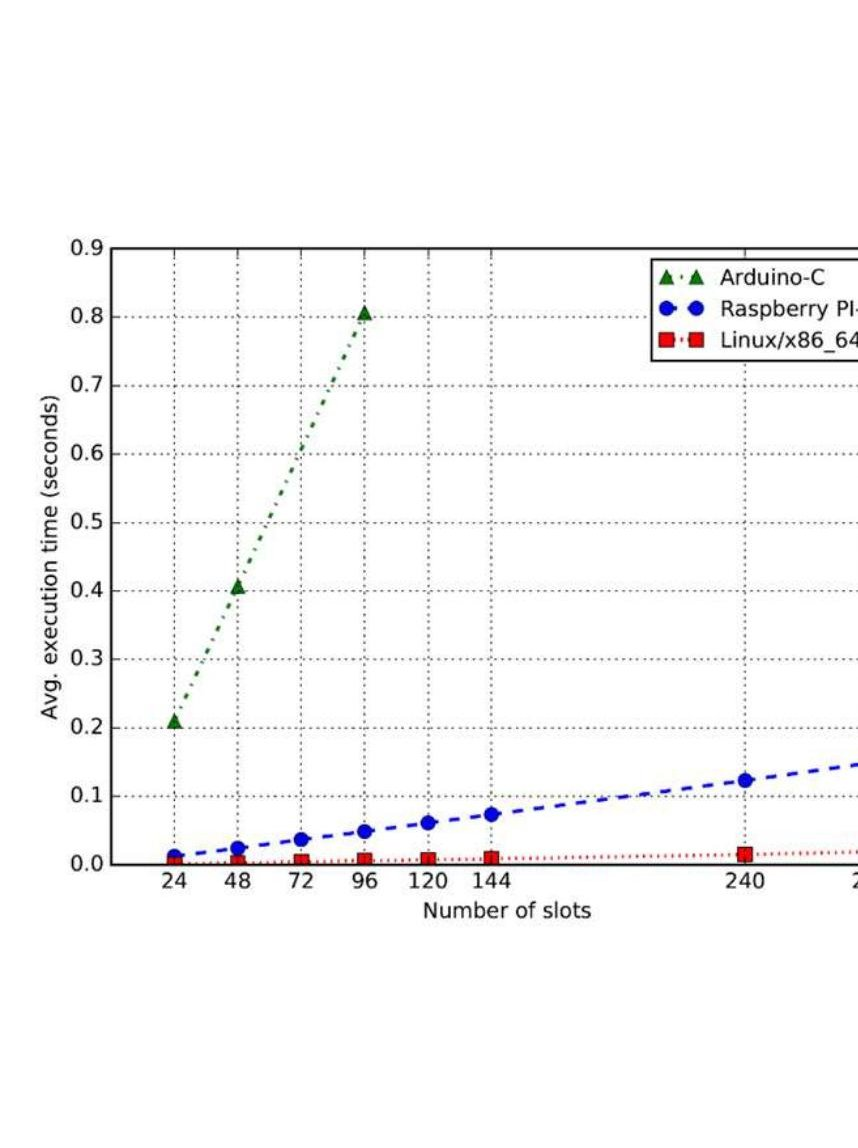
\includegraphics[keepaspectratio]{images/lezione-28-kansal-problem-e-energy-neutrality-img-05.jpg}}
\caption{6 --- Tempo medio di esecuzione del codice C in funzione del
numero di slot. Arduino Uno (verde) scala più rapidamente; Raspberry PI
(blu) rimane entro 0.15 s; Linux x86 (rosso) è pressoché piatto.
Batteria da 2000 mAh, ADC 10 bit, 197 livelli.}
\end{figure}

\subsection{Simulazioni (Piattaforma
Tmote)}\label{simulazioni-piattaforma-tmote}

I test simulano applicazioni con duty cycle tra 2\% e 46\% su batteria
KL-SUN3W da 2000 mAh, variando il numero di slot da 24 a 288, per tutti
i mesi dell'anno.

\begin{figure}
\centering
\pandocbounded{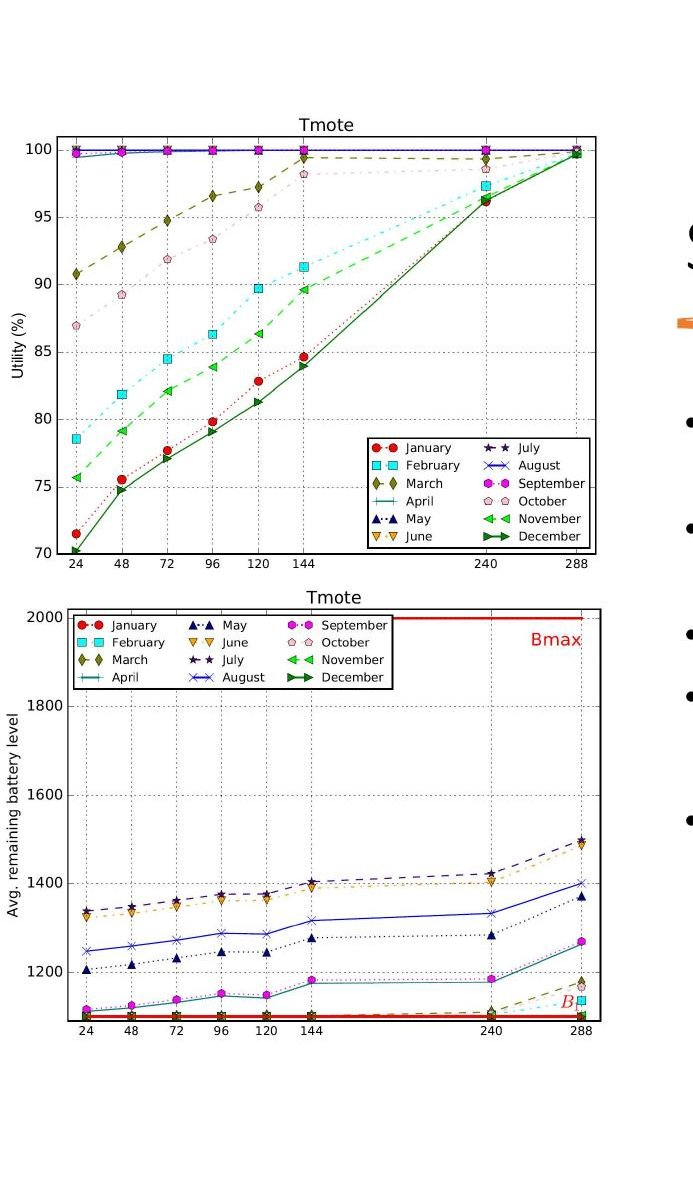
\includegraphics[keepaspectratio]{images/lezione-28-kansal-problem-e-energy-neutrality-img-06.jpg}}
\caption{7 --- In alto: utility percentuale per mese al variare del
numero di slot (tutti i mesi convergono a 100\% con slot sufficienti).
In basso: livello medio di batteria residua (rimane ben sopra
\(B_{min}\), garantendo neutralità energetica).}
\end{figure}

\begin{figure}
\centering
\pandocbounded{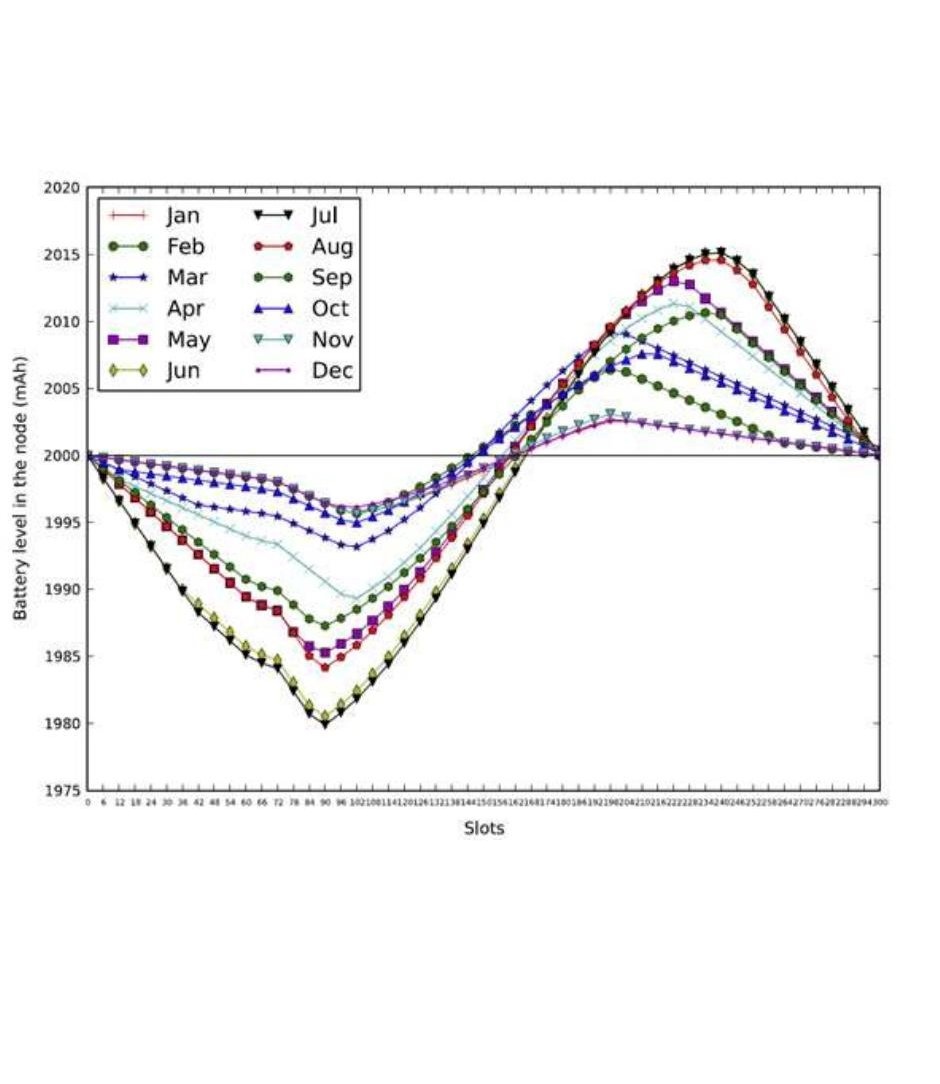
\includegraphics[keepaspectratio]{images/lezione-28-kansal-problem-e-energy-neutrality-img-07.jpg}}
\caption{8 --- Andamento del livello di batteria nel corso della
giornata per mese: scende durante le ore notturne, risale durante le ore
di sole. In estate l'escursione è minima; in inverno è massima ma rimane
entro i limiti ammissibili.}
\end{figure}

\begin{center}\rule{0.5\linewidth}{0.5pt}\end{center}

\section{Riferimenti}\label{riferimenti}

\begin{itemize}
\tightlist
\item
  Aman Kansal, Jason Hsu, Sadaf Zahedi, \emph{Power management in energy
  harvesting sensor networks}, ACM Transactions on Embedded Computing
  Systems, 6(4), September 2007.
\item
  A. Caruso, S. Chessa, S. Escolar, X. del Toro, J.C. Carlos López,
  \emph{A Dynamic Programming Algorithm for High-Level Task Scheduling
  in Energy Harvesting IoT}, IEEE Internet of Things Journal,
  5(3):2234--2248 (2018).
\end{itemize}

\begin{center}\rule{0.5\linewidth}{0.5pt}\end{center}

\newpage

\backmatter
\end{document}
